% The whitepaper. Built by `make` in this directory; see README.md.
%
% NO NUMBER IS TYPED INTO A RESULT SECTION BY HAND. Every numeral in the
% sections the number check registers as a result section
% must arrive through \ccnum{key}, and every key must resolve in
% generated/numbers.tex, which the number generator
% writes from committed records. The Makefile runs the check before latexmk,
% so a hand-typed figure fails the build rather than reaching a reader.
\documentclass[11pt]{article}
% Packages, and the two macros the number pipeline depends on.
\usepackage[utf8]{inputenc}
\usepackage[T1]{fontenc}
\usepackage[margin=1in]{geometry}
\usepackage{microtype}
\usepackage{amsmath}
\usepackage{booktabs}
\usepackage{graphicx}
\usepackage{caption}
\usepackage{float}
\usepackage{listings}
\usepackage[numbers]{natbib}
\usepackage{xcolor}
% Links show in the text itself, on screen and on paper: one dark blue for
% cross-references, citations and web addresses. With `hidelinks` a reference
% was a link only to a reader who happened to hover over it.
\definecolor{linkblue}{RGB}{0,51,153}
\usepackage[colorlinks=true,linkcolor=linkblue,citecolor=linkblue,urlcolor=linkblue]{hyperref}
\usepackage{pgfplots}
\pgfplotsset{compat=1.18}

% The figures' palette and styles, shared by the five diagrams and charts in
% sections/fig-*.tex. One meaning per colour, the same in every figure: blue is
% a program, orange a model (in the charts, Anthropic; teal is OpenAI), green a
% good outcome, red a finding.
\usetikzlibrary{arrows.meta,positioning,fit,shapes.geometric,calc,shadows}
\definecolor{progblue}{RGB}{33,102,172}
\definecolor{progfill}{RGB}{222,235,247}
\definecolor{modelorange}{RGB}{204,102,0}
\definecolor{modelfill}{RGB}{254,235,212}
\definecolor{goodgreen}{RGB}{35,139,69}
\definecolor{goodfill}{RGB}{229,245,224}
\definecolor{badred}{RGB}{203,24,29}
\definecolor{badfill}{RGB}{254,224,210}
\definecolor{docgrey}{RGB}{90,90,90}
\definecolor{docfill}{RGB}{245,245,245}
% Vendors in the charts.
\definecolor{anthropic}{RGB}{204,102,0}
\definecolor{openai}{RGB}{16,130,120}
\tikzset{
  doc/.style={draw=docgrey, fill=docfill, rounded corners=2pt, align=center,
              font=\small, inner sep=5pt, drop shadow={opacity=0.15}},
  prog/.style={draw=progblue, fill=progfill, thick, rounded corners=3pt, align=center,
               font=\small, inner sep=5pt},
  model/.style={draw=modelorange, fill=modelfill, thick, rounded corners=3pt, align=center,
                font=\small, inner sep=5pt},
  good/.style={draw=goodgreen, fill=goodfill, thick, rounded corners=3pt, align=center,
               font=\small, inner sep=5pt},
  bad/.style={draw=badred, fill=badfill, thick, rounded corners=3pt, align=center,
              font=\small, inner sep=5pt},
  ask/.style={draw=progblue, fill=progfill, thick, diamond, aspect=2.4, align=center,
              font=\footnotesize, inner sep=1pt},
  flow/.style={-{Stealth[length=6pt]}, thick, draw=docgrey},
  lbl/.style={font=\footnotesize\itshape, text=docgrey},
}

% Tables and figures.
%
% Every table and figure is placed with [H], exactly where its source stands,
% between two paragraphs. A float that LaTeX moves to the top of a page lands
% in the middle of whatever sentence was running there, and a caption followed
% by the second half of a sentence from the page before reads as broken text.
%
% A caption is set apart from the body: smaller type, indented on both sides, a
% bold label, and a thin rule below it (`\floatfoot`, written after each
% caption) before the text resumes.
\captionsetup{font=footnotesize,labelfont=bf,margin=0.06\linewidth,skip=8pt}
\setlength{\intextsep}{16pt plus 4pt minus 4pt}
\newcommand{\floatfoot}{\par\vspace{7pt}{\centering\rule{0.4\linewidth}{0.3pt}\par}}

% A compact word list for "Words used in this paper". Defined here because a
% result section may not carry a digit, and a length is written with one.
\newenvironment{wordlist}{%
  \begin{description}%
    \setlength{\itemsep}{1pt}\setlength{\parskip}{0pt}\setlength{\parsep}{0pt}}%
  {\end{description}}
% The same for a bullet list.
\newenvironment{points}{%
  \begin{itemize}%
    \setlength{\itemsep}{2pt}\setlength{\parskip}{0pt}\setlength{\parsep}{0pt}}%
  {\end{itemize}}

% -- the number pipeline ----------------------------------------------------
%
% generated/numbers.tex defines one \ccval@<key> per measured figure. \ccnum
% is the only way a numeral is allowed to enter a result section, and it fails
% loudly rather than typesetting a question mark: an undefined key is a figure
% somebody deleted from the records, and a paper that renders anyway is a paper
% that ships a hole.
\makeatletter
\newcommand{\ccnum}[1]{%
  \@ifundefined{ccval@#1}%
    {\PackageError{llossless}{No generated value for key '#1'}%
      {Run `make numbers` -- generated/numbers.tex is stale or the key is misspelt.}}%
    {\csname ccval@#1\endcsname}%
}
% \ccplanned names an arm that has NOT been run. It renders exactly as \ccnum
% does -- the reader sees a model name either way -- and it exists so that the
% difference is machine-checkable. `\ccnum` asserts "a record under
% paper/records/ carries this arm"; `\ccplanned` asserts the opposite, on
% purpose, so a section can say what has not been measured without the claim
% reading as a measurement. check_numbers.py refuses each one used for the
% other's job, so neither marker can rot into a lie as arms are run.
\newcommand{\ccplanned}[1]{%
  \@ifundefined{ccval@#1}%
    {\PackageError{llossless}{No generated value for key '#1'}%
      {Run `make numbers` -- generated/numbers.tex is stale or the key is misspelt.}}%
    {\csname ccval@#1\endcsname}%
}
\makeatother
\IfFileExists{generated/numbers.tex}{% GENERATED by paper/figures/build_numbers.py. Do not edit.
% A hand edit here is a hand-typed number one indirection further away,
% which is worse than the thing check_numbers.py exists to stop.
% Provenance per key, including the record sha256: generated/numbers.json
\makeatletter
\expandafter\def\csname ccval@annotated.pages\endcsname{7}
\expandafter\def\csname ccval@b5.absent\endcsname{6}
\expandafter\def\csname ccval@b5.absent_chars\endcsname{301}
\expandafter\def\csname ccval@b5.absent_chars_percent\endcsname{88}
\expandafter\def\csname ccval@b5.absent_percent\endcsname{75}
\expandafter\def\csname ccval@b5.declared_drops\endcsname{0}
\expandafter\def\csname ccval@b5.fan_in\endcsname{6}
\expandafter\def\csname ccval@b5.findings\endcsname{1}
\expandafter\def\csname ccval@b5.levels\endcsname{6}
\expandafter\def\csname ccval@b5.merged_chars\endcsname{104}
\expandafter\def\csname ccval@b5.pairs\endcsname{9}
\expandafter\def\csname ccval@b5.pairs_max_fan_in\endcsname{2}
\expandafter\def\csname ccval@b5.pairs_max_fan_in_registered\endcsname{3}
\expandafter\def\csname ccval@b5.pairs_supersessions\endcsname{96}
\expandafter\def\csname ccval@b5.records\endcsname{333}
\expandafter\def\csname ccval@b5.reference_firing_pairs\endcsname{8}
\expandafter\def\csname ccval@b5.reference_firings\endcsname{32}
\expandafter\def\csname ccval@b5.reference_percent\endcsname{32.7}
\expandafter\def\csname ccval@b5.reference_records\endcsname{98}
\expandafter\def\csname ccval@b5.segments\endcsname{8}
\expandafter\def\csname ccval@b5.similarity_cassettes\endcsname{9}
\expandafter\def\csname ccval@b5.similarity_firings\endcsname{42}
\expandafter\def\csname ccval@b5.similarity_floor\endcsname{0.373}
\expandafter\def\csname ccval@b5.similarity_percent\endcsname{12.6}
\expandafter\def\csname ccval@b5.source_chars\endcsname{341}
\expandafter\def\csname ccval@b5.split_declared_drops\endcsname{0}
\expandafter\def\csname ccval@b5.split_findings\endcsname{0}
\expandafter\def\csname ccval@b5.split_spans\endcsname{6}
\expandafter\def\csname ccval@b5.subsumed_p5\endcsname{0.000}
\expandafter\def\csname ccval@b5.test\endcsname{test\_b5\_declaring\_your\_way\_past\_the\_checks\_still\_works}
\expandafter\def\csname ccval@bench.k5replication.honesty_k5.declared_drops.max\endcsname{3}
\expandafter\def\csname ccval@bench.k5replication.honesty_k5.declared_drops.median\endcsname{3}
\expandafter\def\csname ccval@bench.k5replication.honesty_k5.declared_drops.min\endcsname{0}
\expandafter\def\csname ccval@bench.k5replication.honesty_k5.distinct_merges\endcsname{2}
\expandafter\def\csname ccval@bench.k5replication.honesty_k5.draws\endcsname{5}
\expandafter\def\csname ccval@bench.k5replication.honesty_k5.draws_declaring_drop\endcsname{4}
\expandafter\def\csname ccval@bench.k5replication.honesty_k5.draws_over_budget\endcsname{0}
\expandafter\def\csname ccval@blindspot.after_named\endcsname{17}
\expandafter\def\csname ccval@blindspot.before_named\endcsname{3}
\expandafter\def\csname ccval@blindspot.total\endcsname{20}
\expandafter\def\csname ccval@build.commit\endcsname{6d5a655833b1}
\expandafter\def\csname ccval@build.digest\endcsname{43fda72e9e49}
\expandafter\def\csname ccval@build.digest.full\endcsname{43fda72e9e4929e59117fa75c517d8462ad6cade1f7f32c8bc4ebce4903cdd1f}
\expandafter\def\csname ccval@build.tag\endcsname{untagged}
\expandafter\def\csname ccval@corpus.detection_block\endcsname{13}
\expandafter\def\csname ccval@corpus.fixtures\endcsname{16}
\expandafter\def\csname ccval@corpus.handwritten\endcsname{19}
\expandafter\def\csname ccval@corpus.largest_pair.name\endcsname{rate\_limits}
\expandafter\def\csname ccval@corpus.largest_pair.segments\endcsname{104}
\expandafter\def\csname ccval@corpus.largest_pair.sources\endcsname{2}
\expandafter\def\csname ccval@corpus.largest_pair.words\endcsname{1,809}
\expandafter\def\csname ccval@corpus.largest_set.name\endcsname{mahjongg}
\expandafter\def\csname ccval@corpus.largest_set.segments\endcsname{216}
\expandafter\def\csname ccval@corpus.largest_set.sources\endcsname{3}
\expandafter\def\csname ccval@corpus.largest_set.words\endcsname{3,602}
\expandafter\def\csname ccval@corpus.mahjongg.sources\endcsname{3}
\expandafter\def\csname ccval@corpus.pairs\endcsname{9}
\expandafter\def\csname ccval@corrected.A-27b.disqualified_as_run_count\endcsname{1}
\expandafter\def\csname ccval@corrected.A-27b.disqualified_count\endcsname{2}
\expandafter\def\csname ccval@corrected.A-27b.exit_code_matched_count\endcsname{12}
\expandafter\def\csname ccval@corrected.A-27b.exit_code_missed_count\endcsname{1}
\expandafter\def\csname ccval@corrected.A-27b.exit_code_unmeasured_count\endcsname{0}
\expandafter\def\csname ccval@corrected.A-27b.fixtures\endcsname{13}
\expandafter\def\csname ccval@corrected.A-27b.fixtures_measured\endcsname{13}
\expandafter\def\csname ccval@corrected.A-27b.invented_total\endcsname{1}
\expandafter\def\csname ccval@corrected.A-27b.model\endcsname{qwen3.8:27b}
\expandafter\def\csname ccval@corrected.A-27b.plants_detected\endcsname{7}
\expandafter\def\csname ccval@corrected.A-27b.plants_total\endcsname{7}
\expandafter\def\csname ccval@corrected.B-70b.disqualified_as_run_count\endcsname{0}
\expandafter\def\csname ccval@corrected.B-70b.disqualified_count\endcsname{0}
\expandafter\def\csname ccval@corrected.B-70b.exit_code_matched_count\endcsname{12}
\expandafter\def\csname ccval@corrected.B-70b.exit_code_missed_count\endcsname{0}
\expandafter\def\csname ccval@corrected.B-70b.exit_code_unmeasured_count\endcsname{1}
\expandafter\def\csname ccval@corrected.B-70b.fixtures\endcsname{13}
\expandafter\def\csname ccval@corrected.B-70b.fixtures_measured\endcsname{12}
\expandafter\def\csname ccval@corrected.B-70b.invented_total\endcsname{0}
\expandafter\def\csname ccval@corrected.B-70b.model\endcsname{deepseek-r1:70b}
\expandafter\def\csname ccval@corrected.B-70b.plants_detected\endcsname{6}
\expandafter\def\csname ccval@corrected.B-70b.plants_total\endcsname{7}
\expandafter\def\csname ccval@corrected.C-120b.disqualified_as_run_count\endcsname{2}
\expandafter\def\csname ccval@corrected.C-120b.disqualified_count\endcsname{3}
\expandafter\def\csname ccval@corrected.C-120b.exit_code_matched_count\endcsname{11}
\expandafter\def\csname ccval@corrected.C-120b.exit_code_missed_count\endcsname{2}
\expandafter\def\csname ccval@corrected.C-120b.exit_code_unmeasured_count\endcsname{0}
\expandafter\def\csname ccval@corrected.C-120b.fixtures\endcsname{13}
\expandafter\def\csname ccval@corrected.C-120b.fixtures_measured\endcsname{13}
\expandafter\def\csname ccval@corrected.C-120b.invented_total\endcsname{2}
\expandafter\def\csname ccval@corrected.C-120b.model\endcsname{gpt-oss:120b}
\expandafter\def\csname ccval@corrected.C-120b.plants_detected\endcsname{6}
\expandafter\def\csname ccval@corrected.C-120b.plants_total\endcsname{7}
\expandafter\def\csname ccval@corrected.amended\endcsname{2026-09-03}
\expandafter\def\csname ccval@corrected.arm_count\endcsname{3}
\expandafter\def\csname ccval@corrected.clean_fixtures\endcsname{7}
\expandafter\def\csname ccval@corrected.defect_fixtures\endcsname{6}
\expandafter\def\csname ccval@corrected.swapped_reclassified\endcsname{3}
\expandafter\def\csname ccval@corrected.swapped_unaccounted_as_run\endcsname{4}
\expandafter\def\csname ccval@depth.claimcheck_commit\endcsname{2a01e9b2f242}
\expandafter\def\csname ccval@depth.coverage.as_run.disqualified\endcsname{1}
\expandafter\def\csname ccval@depth.coverage.as_run.guard_wrong_total\endcsname{0}
\expandafter\def\csname ccval@depth.coverage.as_run.invented_total\endcsname{0}
\expandafter\def\csname ccval@depth.coverage.as_run.plants_detected\endcsname{6}
\expandafter\def\csname ccval@depth.coverage.cannot_detect\endcsname{hallucination}
\expandafter\def\csname ccval@depth.coverage.disqualified\endcsname{1}
\expandafter\def\csname ccval@depth.coverage.fixtures\endcsname{13}
\expandafter\def\csname ccval@depth.coverage.guard_confirmed_total\endcsname{90}
\expandafter\def\csname ccval@depth.coverage.guard_probes_total\endcsname{118}
\expandafter\def\csname ccval@depth.coverage.guard_unclaimed_total\endcsname{28}
\expandafter\def\csname ccval@depth.coverage.guard_wrong_total\endcsname{0}
\expandafter\def\csname ccval@depth.coverage.invented_total\endcsname{0}
\expandafter\def\csname ccval@depth.coverage.merged_to_sources.guards\endcsname{28}
\expandafter\def\csname ccval@depth.coverage.merged_to_sources.guards_graded\endcsname{0}
\expandafter\def\csname ccval@depth.coverage.merged_to_sources.guards_wrong\endcsname{0}
\expandafter\def\csname ccval@depth.coverage.merged_to_sources.plants\endcsname{3}
\expandafter\def\csname ccval@depth.coverage.merged_to_sources.plants_detected\endcsname{3}
\expandafter\def\csname ccval@depth.coverage.merged_to_sources.plants_detected_mechanically\endcsname{3}
\expandafter\def\csname ccval@depth.coverage.model_calls\endcsname{26}
\expandafter\def\csname ccval@depth.coverage.plants_detected\endcsname{6}
\expandafter\def\csname ccval@depth.coverage.plants_total\endcsname{7}
\expandafter\def\csname ccval@depth.coverage.second_reports_total\endcsname{0}
\expandafter\def\csname ccval@depth.coverage.seconds\endcsname{1432.8}
\expandafter\def\csname ccval@depth.coverage.source_to_merged.guards\endcsname{90}
\expandafter\def\csname ccval@depth.coverage.source_to_merged.guards_graded\endcsname{90}
\expandafter\def\csname ccval@depth.coverage.source_to_merged.guards_wrong\endcsname{0}
\expandafter\def\csname ccval@depth.coverage.source_to_merged.plants\endcsname{3}
\expandafter\def\csname ccval@depth.coverage.source_to_merged.plants_detected\endcsname{3}
\expandafter\def\csname ccval@depth.coverage.source_to_merged.plants_detected_mechanically\endcsname{0}
\expandafter\def\csname ccval@depth.coverage.speedup\endcsname{2.04}
\expandafter\def\csname ccval@depth.draws\endcsname{1}
\expandafter\def\csname ccval@depth.fixtures\endcsname{13}
\expandafter\def\csname ccval@depth.full.as_run.disqualified\endcsname{1}
\expandafter\def\csname ccval@depth.full.as_run.guard_wrong_total\endcsname{0}
\expandafter\def\csname ccval@depth.full.as_run.invented_total\endcsname{2}
\expandafter\def\csname ccval@depth.full.as_run.plants_detected\endcsname{7}
\expandafter\def\csname ccval@depth.full.disqualified\endcsname{0}
\expandafter\def\csname ccval@depth.full.fixtures\endcsname{13}
\expandafter\def\csname ccval@depth.full.guard_confirmed_total\endcsname{116}
\expandafter\def\csname ccval@depth.full.guard_probes_total\endcsname{118}
\expandafter\def\csname ccval@depth.full.guard_unclaimed_total\endcsname{2}
\expandafter\def\csname ccval@depth.full.guard_wrong_total\endcsname{0}
\expandafter\def\csname ccval@depth.full.invented_total\endcsname{0}
\expandafter\def\csname ccval@depth.full.merged_to_sources.guards\endcsname{28}
\expandafter\def\csname ccval@depth.full.merged_to_sources.guards_graded\endcsname{28}
\expandafter\def\csname ccval@depth.full.merged_to_sources.guards_wrong\endcsname{0}
\expandafter\def\csname ccval@depth.full.merged_to_sources.plants\endcsname{4}
\expandafter\def\csname ccval@depth.full.merged_to_sources.plants_detected\endcsname{4}
\expandafter\def\csname ccval@depth.full.merged_to_sources.plants_detected_mechanically\endcsname{1}
\expandafter\def\csname ccval@depth.full.model_calls\endcsname{71}
\expandafter\def\csname ccval@depth.full.plants_detected\endcsname{7}
\expandafter\def\csname ccval@depth.full.plants_total\endcsname{7}
\expandafter\def\csname ccval@depth.full.second_reports_total\endcsname{2}
\expandafter\def\csname ccval@depth.full.seconds\endcsname{2924.2}
\expandafter\def\csname ccval@depth.full.source_to_merged.guards\endcsname{90}
\expandafter\def\csname ccval@depth.full.source_to_merged.guards_graded\endcsname{88}
\expandafter\def\csname ccval@depth.full.source_to_merged.guards_wrong\endcsname{0}
\expandafter\def\csname ccval@depth.full.source_to_merged.plants\endcsname{3}
\expandafter\def\csname ccval@depth.full.source_to_merged.plants_detected\endcsname{3}
\expandafter\def\csname ccval@depth.full.source_to_merged.plants_detected_mechanically\endcsname{0}
\expandafter\def\csname ccval@depth.measured_on\endcsname{2026-09-24}
\expandafter\def\csname ccval@depth.model\endcsname{Qwen/Qwen3.8-27B-FP8}
\expandafter\def\csname ccval@depth.plants\endcsname{7}
\expandafter\def\csname ccval@detect.A-27b.exit_code_matched\endcsname{11}
\expandafter\def\csname ccval@detect.A-27b.exit_code_missed\endcsname{2}
\expandafter\def\csname ccval@detect.A-27b.fixtures\endcsname{13}
\expandafter\def\csname ccval@detect.A-27b.invented_total\endcsname{2}
\expandafter\def\csname ccval@detect.A-27b.model\endcsname{qwen3.8:27b}
\expandafter\def\csname ccval@detect.A-27b.plants_detected\endcsname{6}
\expandafter\def\csname ccval@detect.A-27b.plants_missed\endcsname{0}
\expandafter\def\csname ccval@detect.A-27b.plants_total\endcsname{6}
\expandafter\def\csname ccval@detect.B-70b.exit_code_matched\endcsname{11}
\expandafter\def\csname ccval@detect.B-70b.exit_code_missed\endcsname{2}
\expandafter\def\csname ccval@detect.B-70b.fixtures\endcsname{13}
\expandafter\def\csname ccval@detect.B-70b.invented_total\endcsname{1}
\expandafter\def\csname ccval@detect.B-70b.model\endcsname{deepseek-r1:70b}
\expandafter\def\csname ccval@detect.B-70b.plants_detected\endcsname{5}
\expandafter\def\csname ccval@detect.B-70b.plants_missed\endcsname{1}
\expandafter\def\csname ccval@detect.B-70b.plants_total\endcsname{6}
\expandafter\def\csname ccval@detect.C-120b.exit_code_matched\endcsname{13}
\expandafter\def\csname ccval@detect.C-120b.exit_code_missed\endcsname{0}
\expandafter\def\csname ccval@detect.C-120b.fixtures\endcsname{13}
\expandafter\def\csname ccval@detect.C-120b.invented_total\endcsname{3}
\expandafter\def\csname ccval@detect.C-120b.model\endcsname{gpt-oss:120b}
\expandafter\def\csname ccval@detect.C-120b.plants_detected\endcsname{6}
\expandafter\def\csname ccval@detect.C-120b.plants_missed\endcsname{0}
\expandafter\def\csname ccval@detect.C-120b.plants_total\endcsname{6}
\expandafter\def\csname ccval@fd.departed_records\endcsname{29}
\expandafter\def\csname ccval@fd.excluded\endcsname{2}
\expandafter\def\csname ccval@fd.findings\endcsname{15}
\expandafter\def\csname ccval@fd.records\endcsname{30}
\expandafter\def\csname ccval@fd.segments\endcsname{63}
\expandafter\def\csname ccval@lineup.amended.date\endcsname{2026-10-12}
\expandafter\def\csname ccval@lineup.amendments.after_results\endcsname{4}
\expandafter\def\csname ccval@lineup.amendments.before_calls\endcsname{2}
\expandafter\def\csname ccval@lineup.amendments.last\endcsname{6}
\expandafter\def\csname ccval@lineup.amendments.last_date\endcsname{2026-10-15}
\expandafter\def\csname ccval@lineup.audit.all.cases\endcsname{65}
\expandafter\def\csname ccval@lineup.audit.all.gone\endcsname{2}
\expandafter\def\csname ccval@lineup.audit.all.headings_untaken\endcsname{12}
\expandafter\def\csname ccval@lineup.audit.all.lost\endcsname{11}
\expandafter\def\csname ccval@lineup.audit.all.lost_cleared\endcsname{0}
\expandafter\def\csname ccval@lineup.audit.all.lost_still_counted\endcsname{11}
\expandafter\def\csname ccval@lineup.audit.all.not_content\endcsname{12}
\expandafter\def\csname ccval@lineup.audit.all.partly\endcsname{9}
\expandafter\def\csname ccval@lineup.audit.all.present\endcsname{42}
\expandafter\def\csname ccval@lineup.audit.all.present_found\endcsname{8}
\expandafter\def\csname ccval@lineup.audit.all.present_still_counted\endcsname{34}
\expandafter\def\csname ccval@lineup.audit.all.still_counted\endcsname{45}
\expandafter\def\csname ccval@lineup.audit.all.still_there\endcsname{54}
\expandafter\def\csname ccval@lineup.audit.borderline.cases\endcsname{12}
\expandafter\def\csname ccval@lineup.audit.borderline.first\endcsname{4}
\expandafter\def\csname ccval@lineup.audit.borderline.verdict_row\endcsname{gpt-6-luna-api}
\expandafter\def\csname ccval@lineup.audit.borderline.verdicts_moved\endcsname{1}
\expandafter\def\csname ccval@lineup.audit.both.borderline.cases\endcsname{19}
\expandafter\def\csname ccval@lineup.audit.both.borderline.first\endcsname{11}
\expandafter\def\csname ccval@lineup.audit.both.cases\endcsname{84}
\expandafter\def\csname ccval@lineup.audit.both.first.cases\endcsname{44}
\expandafter\def\csname ccval@lineup.audit.both.first.gone\endcsname{1}
\expandafter\def\csname ccval@lineup.audit.both.first.lost\endcsname{6}
\expandafter\def\csname ccval@lineup.audit.both.first.not_content\endcsname{12}
\expandafter\def\csname ccval@lineup.audit.both.first.partly\endcsname{5}
\expandafter\def\csname ccval@lineup.audit.both.first.present\endcsname{26}
\expandafter\def\csname ccval@lineup.audit.both.first.still_there\endcsname{38}
\expandafter\def\csname ccval@lineup.audit.both.runs\endcsname{21}
\expandafter\def\csname ccval@lineup.audit.both.second.cases\endcsname{44}
\expandafter\def\csname ccval@lineup.audit.both.second.same_class\endcsname{42}
\expandafter\def\csname ccval@lineup.audit.date\endcsname{2026-10-12}
\expandafter\def\csname ccval@lineup.audit.example.author_api.class\endcsname{partly}
\expandafter\def\csname ccval@lineup.audit.example.author_api.pair\endcsname{trace\_names}
\expandafter\def\csname ccval@lineup.audit.example.author_api.readings_naming_present\endcsname{0}
\expandafter\def\csname ccval@lineup.audit.example.author_api.row\endcsname{haiku-4.5-api}
\expandafter\def\csname ccval@lineup.audit.example.author_api.segment\endcsname{b2}
\expandafter\def\csname ccval@lineup.audit.example.author_sub.class\endcsname{gone}
\expandafter\def\csname ccval@lineup.audit.example.author_sub.pair\endcsname{trace\_names}
\expandafter\def\csname ccval@lineup.audit.example.author_sub.readings_naming_present\endcsname{0}
\expandafter\def\csname ccval@lineup.audit.example.author_sub.row\endcsname{haiku-4.5-sub}
\expandafter\def\csname ccval@lineup.audit.example.author_sub.segment\endcsname{b2}
\expandafter\def\csname ccval@lineup.audit.example.condition.class\endcsname{partly}
\expandafter\def\csname ccval@lineup.audit.example.condition.heading\endcsname{Placing an item on the shelf}
\expandafter\def\csname ccval@lineup.audit.example.condition.merge\endcsname{Print a hold slip and fold it into the item so the name is visible from the spine.}
\expandafter\def\csname ccval@lineup.audit.example.condition.missing\endcsname{When a requested item arrives}
\expandafter\def\csname ccval@lineup.audit.example.condition.pair\endcsname{library\_holds}
\expandafter\def\csname ccval@lineup.audit.example.condition.readings_naming_present\endcsname{2}
\expandafter\def\csname ccval@lineup.audit.example.condition.row\endcsname{gpt-6-luna-api}
\expandafter\def\csname ccval@lineup.audit.example.condition.segment\endcsname{a3}
\expandafter\def\csname ccval@lineup.audit.example.condition.source\endcsname{When a requested item arrives, print a hold slip and fold it into the item so the name is visible from the spine.}
\expandafter\def\csname ccval@lineup.audit.example.heading.merge\endcsname{How to retry well}
\expandafter\def\csname ccval@lineup.audit.example.heading.pair\endcsname{rate\_limits}
\expandafter\def\csname ccval@lineup.audit.example.heading.row\endcsname{opus-5.5-api}
\expandafter\def\csname ccval@lineup.audit.example.heading.segment\endcsname{b20}
\expandafter\def\csname ccval@lineup.audit.example.heading.source\endcsname{What the client does}
\expandafter\def\csname ccval@lineup.audit.example.joined.merge\endcsname{Escalate E2 to the workshop after 2 failed attempts; do not keep cycling a dock that has failed twice, since repeated forcing bends the pin and turns a 20 minute workshop job into a replacement.}
\expandafter\def\csname ccval@lineup.audit.example.joined.pair\endcsname{bike\_docks}
\expandafter\def\csname ccval@lineup.audit.example.joined.row\endcsname{sonnet-5-sub}
\expandafter\def\csname ccval@lineup.audit.example.joined.segment\endcsname{a10}
\expandafter\def\csname ccval@lineup.audit.example.joined.source\endcsname{Escalate E2 to the workshop after 2 failed attempts.}
\expandafter\def\csname ccval@lineup.audit.example.partly.merge\endcsname{A station with more than half its docks faulted is taken out of service in the app. Notify the support desk before this happens, not after.}
\expandafter\def\csname ccval@lineup.audit.example.partly.pair\endcsname{bike\_docks}
\expandafter\def\csname ccval@lineup.audit.example.partly.row\endcsname{haiku-4.5-sub}
\expandafter\def\csname ccval@lineup.audit.example.partly.segment\endcsname{b18}
\expandafter\def\csname ccval@lineup.audit.example.partly.source\endcsname{The support desk takes a station out of service in the app when more than half its docks are faulted.}
\expandafter\def\csname ccval@lineup.audit.example.shortened.merge\endcsname{The count follows the credential across hosts.}
\expandafter\def\csname ccval@lineup.audit.example.shortened.pair\endcsname{rate\_limits}
\expandafter\def\csname ccval@lineup.audit.example.shortened.row\endcsname{gpt-6-sol-api}
\expandafter\def\csname ccval@lineup.audit.example.shortened.segment\endcsname{b7}
\expandafter\def\csname ccval@lineup.audit.example.shortened.source\endcsname{The count follows the credential wherever the caller happens to put it, including across hosts.}
\expandafter\def\csname ccval@lineup.audit.extended.date\endcsname{2026-10-12}
\expandafter\def\csname ccval@lineup.audit.first.cases\endcsname{25}
\expandafter\def\csname ccval@lineup.audit.first.gone\endcsname{0}
\expandafter\def\csname ccval@lineup.audit.first.headings_untaken\endcsname{11}
\expandafter\def\csname ccval@lineup.audit.first.lost\endcsname{3}
\expandafter\def\csname ccval@lineup.audit.first.lost_cleared\endcsname{0}
\expandafter\def\csname ccval@lineup.audit.first.lost_still_counted\endcsname{3}
\expandafter\def\csname ccval@lineup.audit.first.not_content\endcsname{11}
\expandafter\def\csname ccval@lineup.audit.first.partly\endcsname{3}
\expandafter\def\csname ccval@lineup.audit.first.present\endcsname{11}
\expandafter\def\csname ccval@lineup.audit.first.present_found\endcsname{4}
\expandafter\def\csname ccval@lineup.audit.first.present_still_counted\endcsname{7}
\expandafter\def\csname ccval@lineup.audit.first.still_counted\endcsname{10}
\expandafter\def\csname ccval@lineup.audit.first.still_there\endcsname{22}
\expandafter\def\csname ccval@lineup.audit.readings\endcsname{4}
\expandafter\def\csname ccval@lineup.audit.reworded.cases\endcsname{19}
\expandafter\def\csname ccval@lineup.audit.reworded.differ\endcsname{0}
\expandafter\def\csname ccval@lineup.audit.reworded.gone\endcsname{1}
\expandafter\def\csname ccval@lineup.audit.reworded.lost\endcsname{3}
\expandafter\def\csname ccval@lineup.audit.reworded.lost_reported\endcsname{3}
\expandafter\def\csname ccval@lineup.audit.reworded.not_content\endcsname{1}
\expandafter\def\csname ccval@lineup.audit.reworded.partly\endcsname{2}
\expandafter\def\csname ccval@lineup.audit.reworded.present\endcsname{15}
\expandafter\def\csname ccval@lineup.audit.reworded.reported\endcsname{19}
\expandafter\def\csname ccval@lineup.audit.reworded.rows\endcsname{4}
\expandafter\def\csname ccval@lineup.audit.reworded.rows_none\endcsname{4}
\expandafter\def\csname ccval@lineup.audit.reworded.runs\endcsname{12}
\expandafter\def\csname ccval@lineup.audit.reworded.same_class\endcsname{19}
\expandafter\def\csname ccval@lineup.audit.rows_disagree\endcsname{0}
\expandafter\def\csname ccval@lineup.audit.rows_lost\endcsname{3}
\expandafter\def\csname ccval@lineup.audit.rows_read\endcsname{5}
\expandafter\def\csname ccval@lineup.audit.runs\endcsname{18}
\expandafter\def\csname ccval@lineup.audit.second.cases\endcsname{25}
\expandafter\def\csname ccval@lineup.audit.second.differ\endcsname{2}
\expandafter\def\csname ccval@lineup.audit.second.lost\endcsname{5}
\expandafter\def\csname ccval@lineup.audit.second.same_class\endcsname{23}
\expandafter\def\csname ccval@lineup.audit.unread.as_run\endcsname{5}
\expandafter\def\csname ccval@lineup.audit.unread.repeats\endcsname{30}
\expandafter\def\csname ccval@lineup.audit.unread.repeats.rows\endcsname{2}
\expandafter\def\csname ccval@lineup.audit.unread.titles\endcsname{2}
\expandafter\def\csname ccval@lineup.cells\endcsname{109}
\expandafter\def\csname ccval@lineup.disqualified\endcsname{3}
\expandafter\def\csname ccval@lineup.fable-sub.S3.bip39.draws\endcsname{0}
\expandafter\def\csname ccval@lineup.fable-sub.S3.mahjongg.draws\endcsname{0}
\expandafter\def\csname ccval@lineup.fable-sub.S3.voyager.draws\endcsname{1}
\expandafter\def\csname ccval@lineup.fable-sub.S3.voyager.max\endcsname{38}
\expandafter\def\csname ccval@lineup.fable-sub.S3.voyager.median\endcsname{38}
\expandafter\def\csname ccval@lineup.fable-sub.S3.voyager.min\endcsname{38}
\expandafter\def\csname ccval@lineup.fable-sub.S3.voyager.total\endcsname{44}
\expandafter\def\csname ccval@lineup.fable-sub.effort\endcsname{medium}
\expandafter\def\csname ccval@lineup.fable-sub.name\endcsname{fable-sub}
\expandafter\def\csname ccval@lineup.failure1.role\endcsname{verify}
\expandafter\def\csname ccval@lineup.failure1.row\endcsname{haiku-4.5-api}
\expandafter\def\csname ccval@lineup.failure2.role\endcsname{merge}
\expandafter\def\csname ccval@lineup.failure2.row\endcsname{haiku-4.5-sub}
\expandafter\def\csname ccval@lineup.first.silent_segments\endcsname{10}
\expandafter\def\csname ccval@lineup.first.untaken\endcsname{11}
\expandafter\def\csname ccval@lineup.fixtures\endcsname{13}
\expandafter\def\csname ccval@lineup.flagged_not_disqualified\endcsname{1}
\expandafter\def\csname ccval@lineup.flagged_rows\endcsname{4}
\expandafter\def\csname ccval@lineup.floor.base_only.dev_per_pair\endcsname{7.56}
\expandafter\def\csname ccval@lineup.floor.base_only.deviations\endcsname{68}
\expandafter\def\csname ccval@lineup.floor.base_only.pairs\endcsname{9}
\expandafter\def\csname ccval@lineup.floor.base_only.silent\endcsname{121}
\expandafter\def\csname ccval@lineup.floor.base_only.silent_per_pair\endcsname{13.44}
\expandafter\def\csname ccval@lineup.floor.base_only.untaken\endcsname{8}
\expandafter\def\csname ccval@lineup.floor.concatenation.dev_per_pair\endcsname{8.78}
\expandafter\def\csname ccval@lineup.floor.concatenation.deviations\endcsname{79}
\expandafter\def\csname ccval@lineup.floor.concatenation.pairs\endcsname{9}
\expandafter\def\csname ccval@lineup.floor.concatenation.silent\endcsname{0}
\expandafter\def\csname ccval@lineup.floor.concatenation.silent_per_pair\endcsname{0.00}
\expandafter\def\csname ccval@lineup.floor.concatenation.untaken\endcsname{0}
\expandafter\def\csname ccval@lineup.floor.union.dev_per_pair\endcsname{7.78}
\expandafter\def\csname ccval@lineup.floor.union.deviations\endcsname{70}
\expandafter\def\csname ccval@lineup.floor.union.pairs\endcsname{9}
\expandafter\def\csname ccval@lineup.floor.union.silent\endcsname{0}
\expandafter\def\csname ccval@lineup.floor.union.silent_per_pair\endcsname{0.00}
\expandafter\def\csname ccval@lineup.floor.union.untaken\endcsname{0}
\expandafter\def\csname ccval@lineup.from\endcsname{2026-09-27}
\expandafter\def\csname ccval@lineup.gpt-6-luna-api.S2.disqualified\endcsname{3}
\expandafter\def\csname ccval@lineup.gpt-6-luna-api.S2.fixtures\endcsname{13}
\expandafter\def\csname ccval@lineup.gpt-6-luna-api.S2.guards_wrong\endcsname{1}
\expandafter\def\csname ccval@lineup.gpt-6-luna-api.S2.invented\endcsname{4}
\expandafter\def\csname ccval@lineup.gpt-6-luna-api.S2.matched\endcsname{10}
\expandafter\def\csname ccval@lineup.gpt-6-luna-api.S2.measured\endcsname{12}
\expandafter\def\csname ccval@lineup.gpt-6-luna-api.S2.order\endcsname{6}
\expandafter\def\csname ccval@lineup.gpt-6-luna-api.S2.plants\endcsname{6}
\expandafter\def\csname ccval@lineup.gpt-6-luna-api.S2.plants_measured\endcsname{6}
\expandafter\def\csname ccval@lineup.gpt-6-luna-api.S2.unmeasured\endcsname{1}
\expandafter\def\csname ccval@lineup.gpt-6-luna-api.S3.bip39.draws\endcsname{3}
\expandafter\def\csname ccval@lineup.gpt-6-luna-api.S3.bip39.max\endcsname{10}
\expandafter\def\csname ccval@lineup.gpt-6-luna-api.S3.bip39.median\endcsname{8}
\expandafter\def\csname ccval@lineup.gpt-6-luna-api.S3.bip39.min\endcsname{7}
\expandafter\def\csname ccval@lineup.gpt-6-luna-api.S3.bip39.total\endcsname{14}
\expandafter\def\csname ccval@lineup.gpt-6-luna-api.S3.fixed_total\endcsname{27}
\expandafter\def\csname ccval@lineup.gpt-6-luna-api.S3.mahjongg.draws\endcsname{1}
\expandafter\def\csname ccval@lineup.gpt-6-luna-api.S3.mahjongg.false\endcsname{0}
\expandafter\def\csname ccval@lineup.gpt-6-luna-api.S3.order\endcsname{3=}
\expandafter\def\csname ccval@lineup.gpt-6-luna-api.S3.voyager.draws\endcsname{3}
\expandafter\def\csname ccval@lineup.gpt-6-luna-api.S3.voyager.max\endcsname{19}
\expandafter\def\csname ccval@lineup.gpt-6-luna-api.S3.voyager.median\endcsname{19}
\expandafter\def\csname ccval@lineup.gpt-6-luna-api.S3.voyager.min\endcsname{18}
\expandafter\def\csname ccval@lineup.gpt-6-luna-api.S3.voyager.total\endcsname{44}
\expandafter\def\csname ccval@lineup.gpt-6-luna-api.audit.all.cases\endcsname{5}
\expandafter\def\csname ccval@lineup.gpt-6-luna-api.audit.all.gone\endcsname{0}
\expandafter\def\csname ccval@lineup.gpt-6-luna-api.audit.all.lost\endcsname{0}
\expandafter\def\csname ccval@lineup.gpt-6-luna-api.audit.all.not_content\endcsname{0}
\expandafter\def\csname ccval@lineup.gpt-6-luna-api.audit.all.partly\endcsname{0}
\expandafter\def\csname ccval@lineup.gpt-6-luna-api.audit.all.present\endcsname{5}
\expandafter\def\csname ccval@lineup.gpt-6-luna-api.audit.all.runs\endcsname{3}
\expandafter\def\csname ccval@lineup.gpt-6-luna-api.audit.borderline_only\endcsname{yes}
\expandafter\def\csname ccval@lineup.gpt-6-luna-api.audit.cases\endcsname{4}
\expandafter\def\csname ccval@lineup.gpt-6-luna-api.audit.counted\endcsname{2}
\expandafter\def\csname ccval@lineup.gpt-6-luna-api.audit.counted.lost\endcsname{0}
\expandafter\def\csname ccval@lineup.gpt-6-luna-api.audit.disqualified\endcsname{yes}
\expandafter\def\csname ccval@lineup.gpt-6-luna-api.audit.found\endcsname{1 of 4}
\expandafter\def\csname ccval@lineup.gpt-6-luna-api.audit.gone\endcsname{0}
\expandafter\def\csname ccval@lineup.gpt-6-luna-api.audit.lost\endcsname{1}
\expandafter\def\csname ccval@lineup.gpt-6-luna-api.audit.lost_borderline\endcsname{1}
\expandafter\def\csname ccval@lineup.gpt-6-luna-api.audit.not_content\endcsname{0}
\expandafter\def\csname ccval@lineup.gpt-6-luna-api.audit.partly\endcsname{1}
\expandafter\def\csname ccval@lineup.gpt-6-luna-api.audit.present\endcsname{3}
\expandafter\def\csname ccval@lineup.gpt-6-luna-api.audit.reworded\endcsname{2}
\expandafter\def\csname ccval@lineup.gpt-6-luna-api.audit.reworded.lost\endcsname{1}
\expandafter\def\csname ccval@lineup.gpt-6-luna-api.audit.second.lost\endcsname{1}
\expandafter\def\csname ccval@lineup.gpt-6-luna-api.dev_per_pair\endcsname{5.44}
\expandafter\def\csname ccval@lineup.gpt-6-luna-api.deviations\endcsname{49}
\expandafter\def\csname ccval@lineup.gpt-6-luna-api.effort\endcsname{medium}
\expandafter\def\csname ccval@lineup.gpt-6-luna-api.list_output_multiple\endcsname{1}
\expandafter\def\csname ccval@lineup.gpt-6-luna-api.model\endcsname{gpt-6-luna}
\expandafter\def\csname ccval@lineup.gpt-6-luna-api.model_failures\endcsname{0}
\expandafter\def\csname ccval@lineup.gpt-6-luna-api.name\endcsname{gpt-6-luna-api}
\expandafter\def\csname ccval@lineup.gpt-6-luna-api.no_better_than_union\endcsname{no}
\expandafter\def\csname ccval@lineup.gpt-6-luna-api.pairs\endcsname{9}
\expandafter\def\csname ccval@lineup.gpt-6-luna-api.pairs_completed\endcsname{9}
\expandafter\def\csname ccval@lineup.gpt-6-luna-api.place\endcsname{disq.}
\expandafter\def\csname ccval@lineup.gpt-6-luna-api.rank\endcsname{disq.}
\expandafter\def\csname ccval@lineup.gpt-6-luna-api.seconds\endcsname{141.3}
\expandafter\def\csname ccval@lineup.gpt-6-luna-api.silent\endcsname{2}
\expandafter\def\csname ccval@lineup.gpt-6-luna-api.silent_per_pair\endcsname{0.22}
\expandafter\def\csname ccval@lineup.gpt-6-luna-api.silent_runs\endcsname{1}
\expandafter\def\csname ccval@lineup.gpt-6-luna-api.spread.badge_access.deviations.max\endcsname{1}
\expandafter\def\csname ccval@lineup.gpt-6-luna-api.spread.badge_access.deviations.median\endcsname{1}
\expandafter\def\csname ccval@lineup.gpt-6-luna-api.spread.badge_access.deviations.min\endcsname{0}
\expandafter\def\csname ccval@lineup.gpt-6-luna-api.spread.badge_access.draws\endcsname{3}
\expandafter\def\csname ccval@lineup.gpt-6-luna-api.spread.badge_access.silent.max\endcsname{0}
\expandafter\def\csname ccval@lineup.gpt-6-luna-api.spread.badge_access.silent.median\endcsname{0}
\expandafter\def\csname ccval@lineup.gpt-6-luna-api.spread.badge_access.silent.min\endcsname{0}
\expandafter\def\csname ccval@lineup.gpt-6-luna-api.spread.rate_limits.deviations.max\endcsname{22}
\expandafter\def\csname ccval@lineup.gpt-6-luna-api.spread.rate_limits.deviations.median\endcsname{18}
\expandafter\def\csname ccval@lineup.gpt-6-luna-api.spread.rate_limits.deviations.min\endcsname{14}
\expandafter\def\csname ccval@lineup.gpt-6-luna-api.spread.rate_limits.draws\endcsname{3}
\expandafter\def\csname ccval@lineup.gpt-6-luna-api.spread.rate_limits.silent.max\endcsname{2}
\expandafter\def\csname ccval@lineup.gpt-6-luna-api.spread.rate_limits.silent.median\endcsname{0}
\expandafter\def\csname ccval@lineup.gpt-6-luna-api.spread.rate_limits.silent.min\endcsname{0}
\expandafter\def\csname ccval@lineup.gpt-6-luna-api.spread.trace_names.deviations.max\endcsname{9}
\expandafter\def\csname ccval@lineup.gpt-6-luna-api.spread.trace_names.deviations.median\endcsname{8}
\expandafter\def\csname ccval@lineup.gpt-6-luna-api.spread.trace_names.deviations.min\endcsname{8}
\expandafter\def\csname ccval@lineup.gpt-6-luna-api.spread.trace_names.draws\endcsname{3}
\expandafter\def\csname ccval@lineup.gpt-6-luna-api.spread.trace_names.silent.max\endcsname{0}
\expandafter\def\csname ccval@lineup.gpt-6-luna-api.spread.trace_names.silent.median\endcsname{0}
\expandafter\def\csname ccval@lineup.gpt-6-luna-api.spread.trace_names.silent.min\endcsname{0}
\expandafter\def\csname ccval@lineup.gpt-6-luna-api.spread_pairs\endcsname{3}
\expandafter\def\csname ccval@lineup.gpt-6-luna-api.story.exit\endcsname{1}
\expandafter\def\csname ccval@lineup.gpt-6-luna-api.story.flagged\endcsname{no}
\expandafter\def\csname ccval@lineup.gpt-6-luna-api.story.kept_a\endcsname{yes}
\expandafter\def\csname ccval@lineup.gpt-6-luna-api.story.kept_b\endcsname{no}
\expandafter\def\csname ccval@lineup.gpt-6-luna-api.tokens\endcsname{39666}
\expandafter\def\csname ccval@lineup.gpt-6-luna-api.union_dev\endcsname{70}
\expandafter\def\csname ccval@lineup.gpt-6-luna-api.unit\endcsname{list}
\expandafter\def\csname ccval@lineup.gpt-6-luna-api.untaken\endcsname{0}
\expandafter\def\csname ccval@lineup.gpt-6-luna-api.untaken_all\endcsname{0}
\expandafter\def\csname ccval@lineup.gpt-6-luna-api.untaken_runs\endcsname{0}
\expandafter\def\csname ccval@lineup.gpt-6-luna-api.usd\endcsname{0.012}
\expandafter\def\csname ccval@lineup.gpt-6-sol-api.S2.disqualified\endcsname{1}
\expandafter\def\csname ccval@lineup.gpt-6-sol-api.S2.fixtures\endcsname{13}
\expandafter\def\csname ccval@lineup.gpt-6-sol-api.S2.guards_wrong\endcsname{0}
\expandafter\def\csname ccval@lineup.gpt-6-sol-api.S2.invented\endcsname{1}
\expandafter\def\csname ccval@lineup.gpt-6-sol-api.S2.matched\endcsname{11}
\expandafter\def\csname ccval@lineup.gpt-6-sol-api.S2.measured\endcsname{12}
\expandafter\def\csname ccval@lineup.gpt-6-sol-api.S2.order\endcsname{4}
\expandafter\def\csname ccval@lineup.gpt-6-sol-api.S2.plants\endcsname{6}
\expandafter\def\csname ccval@lineup.gpt-6-sol-api.S2.plants_measured\endcsname{6}
\expandafter\def\csname ccval@lineup.gpt-6-sol-api.S2.unmeasured\endcsname{1}
\expandafter\def\csname ccval@lineup.gpt-6-sol-api.S3.bip39.draws\endcsname{3}
\expandafter\def\csname ccval@lineup.gpt-6-sol-api.S3.bip39.max\endcsname{12}
\expandafter\def\csname ccval@lineup.gpt-6-sol-api.S3.bip39.median\endcsname{11}
\expandafter\def\csname ccval@lineup.gpt-6-sol-api.S3.bip39.min\endcsname{10}
\expandafter\def\csname ccval@lineup.gpt-6-sol-api.S3.bip39.total\endcsname{14}
\expandafter\def\csname ccval@lineup.gpt-6-sol-api.S3.fixed_total\endcsname{34}
\expandafter\def\csname ccval@lineup.gpt-6-sol-api.S3.mahjongg.draws\endcsname{1}
\expandafter\def\csname ccval@lineup.gpt-6-sol-api.S3.mahjongg.false\endcsname{2}
\expandafter\def\csname ccval@lineup.gpt-6-sol-api.S3.order\endcsname{2=}
\expandafter\def\csname ccval@lineup.gpt-6-sol-api.S3.voyager.draws\endcsname{3}
\expandafter\def\csname ccval@lineup.gpt-6-sol-api.S3.voyager.max\endcsname{29}
\expandafter\def\csname ccval@lineup.gpt-6-sol-api.S3.voyager.median\endcsname{23}
\expandafter\def\csname ccval@lineup.gpt-6-sol-api.S3.voyager.min\endcsname{22}
\expandafter\def\csname ccval@lineup.gpt-6-sol-api.S3.voyager.total\endcsname{44}
\expandafter\def\csname ccval@lineup.gpt-6-sol-api.audit.all.cases\endcsname{1}
\expandafter\def\csname ccval@lineup.gpt-6-sol-api.audit.all.gone\endcsname{0}
\expandafter\def\csname ccval@lineup.gpt-6-sol-api.audit.all.lost\endcsname{0}
\expandafter\def\csname ccval@lineup.gpt-6-sol-api.audit.all.not_content\endcsname{0}
\expandafter\def\csname ccval@lineup.gpt-6-sol-api.audit.all.partly\endcsname{0}
\expandafter\def\csname ccval@lineup.gpt-6-sol-api.audit.all.present\endcsname{1}
\expandafter\def\csname ccval@lineup.gpt-6-sol-api.audit.all.runs\endcsname{1}
\expandafter\def\csname ccval@lineup.gpt-6-sol-api.audit.borderline_only\endcsname{no}
\expandafter\def\csname ccval@lineup.gpt-6-sol-api.audit.cases\endcsname{0}
\expandafter\def\csname ccval@lineup.gpt-6-sol-api.audit.counted\endcsname{0}
\expandafter\def\csname ccval@lineup.gpt-6-sol-api.audit.counted.lost\endcsname{0}
\expandafter\def\csname ccval@lineup.gpt-6-sol-api.audit.disqualified\endcsname{no}
\expandafter\def\csname ccval@lineup.gpt-6-sol-api.audit.found\endcsname{--}
\expandafter\def\csname ccval@lineup.gpt-6-sol-api.audit.gone\endcsname{0}
\expandafter\def\csname ccval@lineup.gpt-6-sol-api.audit.lost\endcsname{0}
\expandafter\def\csname ccval@lineup.gpt-6-sol-api.audit.lost_borderline\endcsname{0}
\expandafter\def\csname ccval@lineup.gpt-6-sol-api.audit.not_content\endcsname{0}
\expandafter\def\csname ccval@lineup.gpt-6-sol-api.audit.partly\endcsname{0}
\expandafter\def\csname ccval@lineup.gpt-6-sol-api.audit.present\endcsname{0}
\expandafter\def\csname ccval@lineup.gpt-6-sol-api.audit.reworded\endcsname{0}
\expandafter\def\csname ccval@lineup.gpt-6-sol-api.audit.reworded.lost\endcsname{0}
\expandafter\def\csname ccval@lineup.gpt-6-sol-api.dev_per_pair\endcsname{3.89}
\expandafter\def\csname ccval@lineup.gpt-6-sol-api.deviations\endcsname{35}
\expandafter\def\csname ccval@lineup.gpt-6-sol-api.effort\endcsname{medium}
\expandafter\def\csname ccval@lineup.gpt-6-sol-api.list_output_multiple\endcsname{20}
\expandafter\def\csname ccval@lineup.gpt-6-sol-api.model\endcsname{gpt-6-sol}
\expandafter\def\csname ccval@lineup.gpt-6-sol-api.model_failures\endcsname{0}
\expandafter\def\csname ccval@lineup.gpt-6-sol-api.name\endcsname{gpt-6-sol-api}
\expandafter\def\csname ccval@lineup.gpt-6-sol-api.no_better_than_union\endcsname{no}
\expandafter\def\csname ccval@lineup.gpt-6-sol-api.pairs\endcsname{9}
\expandafter\def\csname ccval@lineup.gpt-6-sol-api.pairs_completed\endcsname{9}
\expandafter\def\csname ccval@lineup.gpt-6-sol-api.place\endcsname{1}
\expandafter\def\csname ccval@lineup.gpt-6-sol-api.rank\endcsname{1}
\expandafter\def\csname ccval@lineup.gpt-6-sol-api.seconds\endcsname{158.4}
\expandafter\def\csname ccval@lineup.gpt-6-sol-api.silent\endcsname{0}
\expandafter\def\csname ccval@lineup.gpt-6-sol-api.silent_per_pair\endcsname{0.00}
\expandafter\def\csname ccval@lineup.gpt-6-sol-api.silent_runs\endcsname{1}
\expandafter\def\csname ccval@lineup.gpt-6-sol-api.spread.badge_access.deviations.max\endcsname{1}
\expandafter\def\csname ccval@lineup.gpt-6-sol-api.spread.badge_access.deviations.median\endcsname{0}
\expandafter\def\csname ccval@lineup.gpt-6-sol-api.spread.badge_access.deviations.min\endcsname{0}
\expandafter\def\csname ccval@lineup.gpt-6-sol-api.spread.badge_access.draws\endcsname{3}
\expandafter\def\csname ccval@lineup.gpt-6-sol-api.spread.badge_access.silent.max\endcsname{0}
\expandafter\def\csname ccval@lineup.gpt-6-sol-api.spread.badge_access.silent.median\endcsname{0}
\expandafter\def\csname ccval@lineup.gpt-6-sol-api.spread.badge_access.silent.min\endcsname{0}
\expandafter\def\csname ccval@lineup.gpt-6-sol-api.spread.rate_limits.deviations.max\endcsname{9}
\expandafter\def\csname ccval@lineup.gpt-6-sol-api.spread.rate_limits.deviations.median\endcsname{9}
\expandafter\def\csname ccval@lineup.gpt-6-sol-api.spread.rate_limits.deviations.min\endcsname{9}
\expandafter\def\csname ccval@lineup.gpt-6-sol-api.spread.rate_limits.draws\endcsname{3}
\expandafter\def\csname ccval@lineup.gpt-6-sol-api.spread.rate_limits.silent.max\endcsname{1}
\expandafter\def\csname ccval@lineup.gpt-6-sol-api.spread.rate_limits.silent.median\endcsname{0}
\expandafter\def\csname ccval@lineup.gpt-6-sol-api.spread.rate_limits.silent.min\endcsname{0}
\expandafter\def\csname ccval@lineup.gpt-6-sol-api.spread.trace_names.deviations.max\endcsname{10}
\expandafter\def\csname ccval@lineup.gpt-6-sol-api.spread.trace_names.deviations.median\endcsname{9}
\expandafter\def\csname ccval@lineup.gpt-6-sol-api.spread.trace_names.deviations.min\endcsname{8}
\expandafter\def\csname ccval@lineup.gpt-6-sol-api.spread.trace_names.draws\endcsname{3}
\expandafter\def\csname ccval@lineup.gpt-6-sol-api.spread.trace_names.silent.max\endcsname{0}
\expandafter\def\csname ccval@lineup.gpt-6-sol-api.spread.trace_names.silent.median\endcsname{0}
\expandafter\def\csname ccval@lineup.gpt-6-sol-api.spread.trace_names.silent.min\endcsname{0}
\expandafter\def\csname ccval@lineup.gpt-6-sol-api.spread_pairs\endcsname{3}
\expandafter\def\csname ccval@lineup.gpt-6-sol-api.story.exit\endcsname{1}
\expandafter\def\csname ccval@lineup.gpt-6-sol-api.story.flagged\endcsname{yes}
\expandafter\def\csname ccval@lineup.gpt-6-sol-api.story.kept_a\endcsname{yes}
\expandafter\def\csname ccval@lineup.gpt-6-sol-api.story.kept_b\endcsname{no}
\expandafter\def\csname ccval@lineup.gpt-6-sol-api.tokens\endcsname{34956}
\expandafter\def\csname ccval@lineup.gpt-6-sol-api.union_dev\endcsname{70}
\expandafter\def\csname ccval@lineup.gpt-6-sol-api.unit\endcsname{list}
\expandafter\def\csname ccval@lineup.gpt-6-sol-api.untaken\endcsname{0}
\expandafter\def\csname ccval@lineup.gpt-6-sol-api.untaken_all\endcsname{0}
\expandafter\def\csname ccval@lineup.gpt-6-sol-api.untaken_runs\endcsname{0}
\expandafter\def\csname ccval@lineup.gpt-6-sol-api.usd\endcsname{0.189}
\expandafter\def\csname ccval@lineup.haiku-4.5-api.S2.disqualified\endcsname{2}
\expandafter\def\csname ccval@lineup.haiku-4.5-api.S2.fixtures\endcsname{13}
\expandafter\def\csname ccval@lineup.haiku-4.5-api.S2.guards_wrong\endcsname{1}
\expandafter\def\csname ccval@lineup.haiku-4.5-api.S2.invented\endcsname{2}
\expandafter\def\csname ccval@lineup.haiku-4.5-api.S2.matched\endcsname{12}
\expandafter\def\csname ccval@lineup.haiku-4.5-api.S2.measured\endcsname{13}
\expandafter\def\csname ccval@lineup.haiku-4.5-api.S2.order\endcsname{3=}
\expandafter\def\csname ccval@lineup.haiku-4.5-api.S2.plants\endcsname{7}
\expandafter\def\csname ccval@lineup.haiku-4.5-api.S2.plants_measured\endcsname{7}
\expandafter\def\csname ccval@lineup.haiku-4.5-api.S2.unmeasured\endcsname{0}
\expandafter\def\csname ccval@lineup.haiku-4.5-api.S3.bip39.draws\endcsname{3}
\expandafter\def\csname ccval@lineup.haiku-4.5-api.S3.bip39.max\endcsname{9}
\expandafter\def\csname ccval@lineup.haiku-4.5-api.S3.bip39.median\endcsname{8}
\expandafter\def\csname ccval@lineup.haiku-4.5-api.S3.bip39.min\endcsname{8}
\expandafter\def\csname ccval@lineup.haiku-4.5-api.S3.bip39.total\endcsname{14}
\expandafter\def\csname ccval@lineup.haiku-4.5-api.S3.fixed_total\endcsname{19}
\expandafter\def\csname ccval@lineup.haiku-4.5-api.S3.mahjongg.draws\endcsname{1}
\expandafter\def\csname ccval@lineup.haiku-4.5-api.S3.mahjongg.false\endcsname{1}
\expandafter\def\csname ccval@lineup.haiku-4.5-api.S3.order\endcsname{3=}
\expandafter\def\csname ccval@lineup.haiku-4.5-api.S3.voyager.draws\endcsname{3}
\expandafter\def\csname ccval@lineup.haiku-4.5-api.S3.voyager.max\endcsname{18}
\expandafter\def\csname ccval@lineup.haiku-4.5-api.S3.voyager.median\endcsname{11}
\expandafter\def\csname ccval@lineup.haiku-4.5-api.S3.voyager.min\endcsname{6}
\expandafter\def\csname ccval@lineup.haiku-4.5-api.S3.voyager.total\endcsname{44}
\expandafter\def\csname ccval@lineup.haiku-4.5-api.audit.all.cases\endcsname{13}
\expandafter\def\csname ccval@lineup.haiku-4.5-api.audit.all.gone\endcsname{0}
\expandafter\def\csname ccval@lineup.haiku-4.5-api.audit.all.lost\endcsname{1}
\expandafter\def\csname ccval@lineup.haiku-4.5-api.audit.all.not_content\endcsname{9}
\expandafter\def\csname ccval@lineup.haiku-4.5-api.audit.all.partly\endcsname{1}
\expandafter\def\csname ccval@lineup.haiku-4.5-api.audit.all.present\endcsname{3}
\expandafter\def\csname ccval@lineup.haiku-4.5-api.audit.all.runs\endcsname{7}
\expandafter\def\csname ccval@lineup.haiku-4.5-api.audit.borderline_only\endcsname{no}
\expandafter\def\csname ccval@lineup.haiku-4.5-api.audit.cases\endcsname{21}
\expandafter\def\csname ccval@lineup.haiku-4.5-api.audit.counted\endcsname{13}
\expandafter\def\csname ccval@lineup.haiku-4.5-api.audit.counted.lost\endcsname{1}
\expandafter\def\csname ccval@lineup.haiku-4.5-api.audit.disqualified\endcsname{yes}
\expandafter\def\csname ccval@lineup.haiku-4.5-api.audit.found\endcsname{2 of 21}
\expandafter\def\csname ccval@lineup.haiku-4.5-api.audit.gone\endcsname{0}
\expandafter\def\csname ccval@lineup.haiku-4.5-api.audit.lost\endcsname{2}
\expandafter\def\csname ccval@lineup.haiku-4.5-api.audit.lost_borderline\endcsname{1}
\expandafter\def\csname ccval@lineup.haiku-4.5-api.audit.not_content\endcsname{10}
\expandafter\def\csname ccval@lineup.haiku-4.5-api.audit.partly\endcsname{2}
\expandafter\def\csname ccval@lineup.haiku-4.5-api.audit.present\endcsname{9}
\expandafter\def\csname ccval@lineup.haiku-4.5-api.audit.reworded\endcsname{8}
\expandafter\def\csname ccval@lineup.haiku-4.5-api.audit.reworded.lost\endcsname{1}
\expandafter\def\csname ccval@lineup.haiku-4.5-api.audit.second.lost\endcsname{3}
\expandafter\def\csname ccval@lineup.haiku-4.5-api.dev_per_pair\endcsname{6.25}
\expandafter\def\csname ccval@lineup.haiku-4.5-api.deviations\endcsname{50}
\expandafter\def\csname ccval@lineup.haiku-4.5-api.effort\endcsname{one}
\expandafter\def\csname ccval@lineup.haiku-4.5-api.list_output_multiple\endcsname{10}
\expandafter\def\csname ccval@lineup.haiku-4.5-api.model\endcsname{claude-haiku-4-5-20251001}
\expandafter\def\csname ccval@lineup.haiku-4.5-api.model_failures\endcsname{1}
\expandafter\def\csname ccval@lineup.haiku-4.5-api.name\endcsname{haiku-4.5-api}
\expandafter\def\csname ccval@lineup.haiku-4.5-api.no_better_than_union\endcsname{no}
\expandafter\def\csname ccval@lineup.haiku-4.5-api.pairs\endcsname{8}
\expandafter\def\csname ccval@lineup.haiku-4.5-api.pairs_completed\endcsname{8}
\expandafter\def\csname ccval@lineup.haiku-4.5-api.place\endcsname{disq.}
\expandafter\def\csname ccval@lineup.haiku-4.5-api.rank\endcsname{disq.}
\expandafter\def\csname ccval@lineup.haiku-4.5-api.seconds\endcsname{69.1}
\expandafter\def\csname ccval@lineup.haiku-4.5-api.silent\endcsname{3}
\expandafter\def\csname ccval@lineup.haiku-4.5-api.silent_per_pair\endcsname{0.38}
\expandafter\def\csname ccval@lineup.haiku-4.5-api.silent_runs\endcsname{3}
\expandafter\def\csname ccval@lineup.haiku-4.5-api.spread_pairs\endcsname{0}
\expandafter\def\csname ccval@lineup.haiku-4.5-api.story.exit\endcsname{2}
\expandafter\def\csname ccval@lineup.haiku-4.5-api.story.flagged\endcsname{no}
\expandafter\def\csname ccval@lineup.haiku-4.5-api.story.kept_a\endcsname{yes}
\expandafter\def\csname ccval@lineup.haiku-4.5-api.story.kept_b\endcsname{yes}
\expandafter\def\csname ccval@lineup.haiku-4.5-api.tokens\endcsname{30132}
\expandafter\def\csname ccval@lineup.haiku-4.5-api.union_dev\endcsname{64}
\expandafter\def\csname ccval@lineup.haiku-4.5-api.unit\endcsname{list}
\expandafter\def\csname ccval@lineup.haiku-4.5-api.untaken\endcsname{9}
\expandafter\def\csname ccval@lineup.haiku-4.5-api.untaken_all\endcsname{9}
\expandafter\def\csname ccval@lineup.haiku-4.5-api.untaken_runs\endcsname{5}
\expandafter\def\csname ccval@lineup.haiku-4.5-api.usd\endcsname{0.069}
\expandafter\def\csname ccval@lineup.haiku-4.5-sub.S2.disqualified\endcsname{2}
\expandafter\def\csname ccval@lineup.haiku-4.5-sub.S2.fixtures\endcsname{13}
\expandafter\def\csname ccval@lineup.haiku-4.5-sub.S2.guards_wrong\endcsname{1}
\expandafter\def\csname ccval@lineup.haiku-4.5-sub.S2.invented\endcsname{1}
\expandafter\def\csname ccval@lineup.haiku-4.5-sub.S2.matched\endcsname{12}
\expandafter\def\csname ccval@lineup.haiku-4.5-sub.S2.measured\endcsname{13}
\expandafter\def\csname ccval@lineup.haiku-4.5-sub.S2.order\endcsname{2}
\expandafter\def\csname ccval@lineup.haiku-4.5-sub.S2.plants\endcsname{7}
\expandafter\def\csname ccval@lineup.haiku-4.5-sub.S2.plants_measured\endcsname{7}
\expandafter\def\csname ccval@lineup.haiku-4.5-sub.S2.unmeasured\endcsname{0}
\expandafter\def\csname ccval@lineup.haiku-4.5-sub.S3.bip39.draws\endcsname{3}
\expandafter\def\csname ccval@lineup.haiku-4.5-sub.S3.bip39.max\endcsname{9}
\expandafter\def\csname ccval@lineup.haiku-4.5-sub.S3.bip39.median\endcsname{8}
\expandafter\def\csname ccval@lineup.haiku-4.5-sub.S3.bip39.min\endcsname{6}
\expandafter\def\csname ccval@lineup.haiku-4.5-sub.S3.bip39.total\endcsname{14}
\expandafter\def\csname ccval@lineup.haiku-4.5-sub.S3.fixed_total\endcsname{14}
\expandafter\def\csname ccval@lineup.haiku-4.5-sub.S3.mahjongg.draws\endcsname{0}
\expandafter\def\csname ccval@lineup.haiku-4.5-sub.S3.mahjongg.false\endcsname{failed}
\expandafter\def\csname ccval@lineup.haiku-4.5-sub.S3.order\endcsname{3=}
\expandafter\def\csname ccval@lineup.haiku-4.5-sub.S3.voyager.draws\endcsname{3}
\expandafter\def\csname ccval@lineup.haiku-4.5-sub.S3.voyager.max\endcsname{17}
\expandafter\def\csname ccval@lineup.haiku-4.5-sub.S3.voyager.median\endcsname{6}
\expandafter\def\csname ccval@lineup.haiku-4.5-sub.S3.voyager.min\endcsname{2}
\expandafter\def\csname ccval@lineup.haiku-4.5-sub.S3.voyager.total\endcsname{44}
\expandafter\def\csname ccval@lineup.haiku-4.5-sub.audit.all.cases\endcsname{39}
\expandafter\def\csname ccval@lineup.haiku-4.5-sub.audit.all.gone\endcsname{2}
\expandafter\def\csname ccval@lineup.haiku-4.5-sub.audit.all.lost\endcsname{10}
\expandafter\def\csname ccval@lineup.haiku-4.5-sub.audit.all.not_content\endcsname{1}
\expandafter\def\csname ccval@lineup.haiku-4.5-sub.audit.all.partly\endcsname{8}
\expandafter\def\csname ccval@lineup.haiku-4.5-sub.audit.all.present\endcsname{28}
\expandafter\def\csname ccval@lineup.haiku-4.5-sub.audit.all.runs\endcsname{4}
\expandafter\def\csname ccval@lineup.haiku-4.5-sub.audit.borderline_only\endcsname{no}
\expandafter\def\csname ccval@lineup.haiku-4.5-sub.audit.cases\endcsname{8}
\expandafter\def\csname ccval@lineup.haiku-4.5-sub.audit.counted\endcsname{3}
\expandafter\def\csname ccval@lineup.haiku-4.5-sub.audit.counted.lost\endcsname{2}
\expandafter\def\csname ccval@lineup.haiku-4.5-sub.audit.disqualified\endcsname{yes}
\expandafter\def\csname ccval@lineup.haiku-4.5-sub.audit.found\endcsname{3 of 8}
\expandafter\def\csname ccval@lineup.haiku-4.5-sub.audit.gone\endcsname{1}
\expandafter\def\csname ccval@lineup.haiku-4.5-sub.audit.lost\endcsname{3}
\expandafter\def\csname ccval@lineup.haiku-4.5-sub.audit.lost_borderline\endcsname{1}
\expandafter\def\csname ccval@lineup.haiku-4.5-sub.audit.not_content\endcsname{0}
\expandafter\def\csname ccval@lineup.haiku-4.5-sub.audit.partly\endcsname{2}
\expandafter\def\csname ccval@lineup.haiku-4.5-sub.audit.present\endcsname{5}
\expandafter\def\csname ccval@lineup.haiku-4.5-sub.audit.reworded\endcsname{5}
\expandafter\def\csname ccval@lineup.haiku-4.5-sub.audit.reworded.lost\endcsname{1}
\expandafter\def\csname ccval@lineup.haiku-4.5-sub.audit.second.lost\endcsname{4}
\expandafter\def\csname ccval@lineup.haiku-4.5-sub.dev_per_pair\endcsname{7.11}
\expandafter\def\csname ccval@lineup.haiku-4.5-sub.deviations\endcsname{64}
\expandafter\def\csname ccval@lineup.haiku-4.5-sub.model\endcsname{claude-haiku-4-5-20251001}
\expandafter\def\csname ccval@lineup.haiku-4.5-sub.model_failures\endcsname{0}
\expandafter\def\csname ccval@lineup.haiku-4.5-sub.name\endcsname{haiku-4.5-sub}
\expandafter\def\csname ccval@lineup.haiku-4.5-sub.no_better_than_union\endcsname{no}
\expandafter\def\csname ccval@lineup.haiku-4.5-sub.pairs\endcsname{9}
\expandafter\def\csname ccval@lineup.haiku-4.5-sub.pairs_completed\endcsname{9}
\expandafter\def\csname ccval@lineup.haiku-4.5-sub.place\endcsname{disq.}
\expandafter\def\csname ccval@lineup.haiku-4.5-sub.rank\endcsname{disq.}
\expandafter\def\csname ccval@lineup.haiku-4.5-sub.seconds\endcsname{676.5}
\expandafter\def\csname ccval@lineup.haiku-4.5-sub.silent\endcsname{3}
\expandafter\def\csname ccval@lineup.haiku-4.5-sub.silent_per_pair\endcsname{0.33}
\expandafter\def\csname ccval@lineup.haiku-4.5-sub.silent_runs\endcsname{4}
\expandafter\def\csname ccval@lineup.haiku-4.5-sub.spread.badge_access.deviations.max\endcsname{0}
\expandafter\def\csname ccval@lineup.haiku-4.5-sub.spread.badge_access.deviations.median\endcsname{0}
\expandafter\def\csname ccval@lineup.haiku-4.5-sub.spread.badge_access.deviations.min\endcsname{0}
\expandafter\def\csname ccval@lineup.haiku-4.5-sub.spread.badge_access.draws\endcsname{3}
\expandafter\def\csname ccval@lineup.haiku-4.5-sub.spread.badge_access.silent.max\endcsname{0}
\expandafter\def\csname ccval@lineup.haiku-4.5-sub.spread.badge_access.silent.median\endcsname{0}
\expandafter\def\csname ccval@lineup.haiku-4.5-sub.spread.badge_access.silent.min\endcsname{0}
\expandafter\def\csname ccval@lineup.haiku-4.5-sub.spread.rate_limits.deviations.max\endcsname{14}
\expandafter\def\csname ccval@lineup.haiku-4.5-sub.spread.rate_limits.deviations.median\endcsname{9}
\expandafter\def\csname ccval@lineup.haiku-4.5-sub.spread.rate_limits.deviations.min\endcsname{8}
\expandafter\def\csname ccval@lineup.haiku-4.5-sub.spread.rate_limits.draws\endcsname{3}
\expandafter\def\csname ccval@lineup.haiku-4.5-sub.spread.rate_limits.silent.max\endcsname{25}
\expandafter\def\csname ccval@lineup.haiku-4.5-sub.spread.rate_limits.silent.median\endcsname{9}
\expandafter\def\csname ccval@lineup.haiku-4.5-sub.spread.rate_limits.silent.min\endcsname{2}
\expandafter\def\csname ccval@lineup.haiku-4.5-sub.spread.trace_names.deviations.max\endcsname{10}
\expandafter\def\csname ccval@lineup.haiku-4.5-sub.spread.trace_names.deviations.median\endcsname{10}
\expandafter\def\csname ccval@lineup.haiku-4.5-sub.spread.trace_names.deviations.min\endcsname{9}
\expandafter\def\csname ccval@lineup.haiku-4.5-sub.spread.trace_names.draws\endcsname{3}
\expandafter\def\csname ccval@lineup.haiku-4.5-sub.spread.trace_names.silent.max\endcsname{0}
\expandafter\def\csname ccval@lineup.haiku-4.5-sub.spread.trace_names.silent.median\endcsname{0}
\expandafter\def\csname ccval@lineup.haiku-4.5-sub.spread.trace_names.silent.min\endcsname{0}
\expandafter\def\csname ccval@lineup.haiku-4.5-sub.spread_pairs\endcsname{3}
\expandafter\def\csname ccval@lineup.haiku-4.5-sub.story.exit\endcsname{1}
\expandafter\def\csname ccval@lineup.haiku-4.5-sub.story.flagged\endcsname{no}
\expandafter\def\csname ccval@lineup.haiku-4.5-sub.story.kept_a\endcsname{yes}
\expandafter\def\csname ccval@lineup.haiku-4.5-sub.story.kept_b\endcsname{no}
\expandafter\def\csname ccval@lineup.haiku-4.5-sub.tokens\endcsname{122847}
\expandafter\def\csname ccval@lineup.haiku-4.5-sub.union_dev\endcsname{70}
\expandafter\def\csname ccval@lineup.haiku-4.5-sub.unit\endcsname{API-equivalent}
\expandafter\def\csname ccval@lineup.haiku-4.5-sub.untaken\endcsname{0}
\expandafter\def\csname ccval@lineup.haiku-4.5-sub.untaken_all\endcsname{1}
\expandafter\def\csname ccval@lineup.haiku-4.5-sub.untaken_runs\endcsname{1}
\expandafter\def\csname ccval@lineup.haiku-4.5-sub.usd\endcsname{0.483}
\expandafter\def\csname ccval@lineup.licence.bip\endcsname{BIP-39}
\expandafter\def\csname ccval@lineup.licence.bsd\endcsname{12}
\expandafter\def\csname ccval@lineup.licence.bsd_citation\endcsname{12}
\expandafter\def\csname ccval@lineup.licence.bsd_declared\endcsname{12}
\expandafter\def\csname ccval@lineup.licence.bsd_exit\endcsname{1}
\expandafter\def\csname ccval@lineup.licence.bsd_exit_one\endcsname{12}
\expandafter\def\csname ccval@lineup.licence.bsd_name\endcsname{2-clause BSD}
\expandafter\def\csname ccval@lineup.licence.gpl\endcsname{8}
\expandafter\def\csname ccval@lineup.licence.mit\endcsname{2}
\expandafter\def\csname ccval@lineup.licence.none\endcsname{2}
\expandafter\def\csname ccval@lineup.licence.other\endcsname{0}
\expandafter\def\csname ccval@lineup.licence.path\endcsname{tests/handwritten/bip39/}
\expandafter\def\csname ccval@lineup.licence.runs\endcsname{24}
\expandafter\def\csname ccval@lineup.licence.sourced.blind\endcsname{6}
\expandafter\def\csname ccval@lineup.licence.sourced.blind_mit\endcsname{0}
\expandafter\def\csname ccval@lineup.licence.sourced.date\endcsname{2026-09-25}
\expandafter\def\csname ccval@lineup.licence.sourced.looked\endcsname{21}
\expandafter\def\csname ccval@lineup.licence.sourced.looked_mit\endcsname{20}
\expandafter\def\csname ccval@lineup.licence.sourced.runs\endcsname{27}
\expandafter\def\csname ccval@lineup.list_output.lowest\endcsname{gpt-6-luna-api}
\expandafter\def\csname ccval@lineup.opus-5.5-api.S2.disqualified\endcsname{2}
\expandafter\def\csname ccval@lineup.opus-5.5-api.S2.fixtures\endcsname{13}
\expandafter\def\csname ccval@lineup.opus-5.5-api.S2.guards_wrong\endcsname{1}
\expandafter\def\csname ccval@lineup.opus-5.5-api.S2.invented\endcsname{2}
\expandafter\def\csname ccval@lineup.opus-5.5-api.S2.matched\endcsname{12}
\expandafter\def\csname ccval@lineup.opus-5.5-api.S2.measured\endcsname{13}
\expandafter\def\csname ccval@lineup.opus-5.5-api.S2.order\endcsname{3=}
\expandafter\def\csname ccval@lineup.opus-5.5-api.S2.plants\endcsname{7}
\expandafter\def\csname ccval@lineup.opus-5.5-api.S2.plants_measured\endcsname{7}
\expandafter\def\csname ccval@lineup.opus-5.5-api.S2.unmeasured\endcsname{0}
\expandafter\def\csname ccval@lineup.opus-5.5-api.S3.bip39.draws\endcsname{3}
\expandafter\def\csname ccval@lineup.opus-5.5-api.S3.bip39.max\endcsname{13}
\expandafter\def\csname ccval@lineup.opus-5.5-api.S3.bip39.median\endcsname{13}
\expandafter\def\csname ccval@lineup.opus-5.5-api.S3.bip39.min\endcsname{13}
\expandafter\def\csname ccval@lineup.opus-5.5-api.S3.bip39.total\endcsname{14}
\expandafter\def\csname ccval@lineup.opus-5.5-api.S3.fixed_total\endcsname{42}
\expandafter\def\csname ccval@lineup.opus-5.5-api.S3.mahjongg.draws\endcsname{1}
\expandafter\def\csname ccval@lineup.opus-5.5-api.S3.mahjongg.false\endcsname{0}
\expandafter\def\csname ccval@lineup.opus-5.5-api.S3.order\endcsname{1=}
\expandafter\def\csname ccval@lineup.opus-5.5-api.S3.voyager.draws\endcsname{3}
\expandafter\def\csname ccval@lineup.opus-5.5-api.S3.voyager.max\endcsname{32}
\expandafter\def\csname ccval@lineup.opus-5.5-api.S3.voyager.median\endcsname{29}
\expandafter\def\csname ccval@lineup.opus-5.5-api.S3.voyager.min\endcsname{28}
\expandafter\def\csname ccval@lineup.opus-5.5-api.S3.voyager.total\endcsname{44}
\expandafter\def\csname ccval@lineup.opus-5.5-api.audit.all.cases\endcsname{2}
\expandafter\def\csname ccval@lineup.opus-5.5-api.audit.all.gone\endcsname{0}
\expandafter\def\csname ccval@lineup.opus-5.5-api.audit.all.lost\endcsname{0}
\expandafter\def\csname ccval@lineup.opus-5.5-api.audit.all.not_content\endcsname{2}
\expandafter\def\csname ccval@lineup.opus-5.5-api.audit.all.partly\endcsname{0}
\expandafter\def\csname ccval@lineup.opus-5.5-api.audit.all.present\endcsname{0}
\expandafter\def\csname ccval@lineup.opus-5.5-api.audit.all.runs\endcsname{1}
\expandafter\def\csname ccval@lineup.opus-5.5-api.audit.borderline_only\endcsname{no}
\expandafter\def\csname ccval@lineup.opus-5.5-api.audit.cases\endcsname{2}
\expandafter\def\csname ccval@lineup.opus-5.5-api.audit.counted\endcsname{2}
\expandafter\def\csname ccval@lineup.opus-5.5-api.audit.counted.lost\endcsname{0}
\expandafter\def\csname ccval@lineup.opus-5.5-api.audit.disqualified\endcsname{no}
\expandafter\def\csname ccval@lineup.opus-5.5-api.audit.found\endcsname{0 of 2}
\expandafter\def\csname ccval@lineup.opus-5.5-api.audit.gone\endcsname{0}
\expandafter\def\csname ccval@lineup.opus-5.5-api.audit.lost\endcsname{0}
\expandafter\def\csname ccval@lineup.opus-5.5-api.audit.lost_borderline\endcsname{0}
\expandafter\def\csname ccval@lineup.opus-5.5-api.audit.not_content\endcsname{2}
\expandafter\def\csname ccval@lineup.opus-5.5-api.audit.partly\endcsname{0}
\expandafter\def\csname ccval@lineup.opus-5.5-api.audit.present\endcsname{0}
\expandafter\def\csname ccval@lineup.opus-5.5-api.audit.reworded\endcsname{0}
\expandafter\def\csname ccval@lineup.opus-5.5-api.audit.reworded.lost\endcsname{0}
\expandafter\def\csname ccval@lineup.opus-5.5-api.audit.second.lost\endcsname{0}
\expandafter\def\csname ccval@lineup.opus-5.5-api.dev_per_pair\endcsname{5.78}
\expandafter\def\csname ccval@lineup.opus-5.5-api.deviations\endcsname{52}
\expandafter\def\csname ccval@lineup.opus-5.5-api.effort\endcsname{medium}
\expandafter\def\csname ccval@lineup.opus-5.5-api.list_output_multiple\endcsname{40}
\expandafter\def\csname ccval@lineup.opus-5.5-api.model\endcsname{claude-opus-5-5}
\expandafter\def\csname ccval@lineup.opus-5.5-api.model_failures\endcsname{0}
\expandafter\def\csname ccval@lineup.opus-5.5-api.name\endcsname{opus-5.5-api}
\expandafter\def\csname ccval@lineup.opus-5.5-api.no_better_than_union\endcsname{no}
\expandafter\def\csname ccval@lineup.opus-5.5-api.pairs\endcsname{9}
\expandafter\def\csname ccval@lineup.opus-5.5-api.pairs_completed\endcsname{9}
\expandafter\def\csname ccval@lineup.opus-5.5-api.place\endcsname{3}
\expandafter\def\csname ccval@lineup.opus-5.5-api.rank\endcsname{4}
\expandafter\def\csname ccval@lineup.opus-5.5-api.seconds\endcsname{142.7}
\expandafter\def\csname ccval@lineup.opus-5.5-api.silent\endcsname{0}
\expandafter\def\csname ccval@lineup.opus-5.5-api.silent_per_pair\endcsname{0.00}
\expandafter\def\csname ccval@lineup.opus-5.5-api.silent_runs\endcsname{0}
\expandafter\def\csname ccval@lineup.opus-5.5-api.spread.badge_access.deviations.max\endcsname{0}
\expandafter\def\csname ccval@lineup.opus-5.5-api.spread.badge_access.deviations.median\endcsname{0}
\expandafter\def\csname ccval@lineup.opus-5.5-api.spread.badge_access.deviations.min\endcsname{0}
\expandafter\def\csname ccval@lineup.opus-5.5-api.spread.badge_access.draws\endcsname{3}
\expandafter\def\csname ccval@lineup.opus-5.5-api.spread.badge_access.silent.max\endcsname{0}
\expandafter\def\csname ccval@lineup.opus-5.5-api.spread.badge_access.silent.median\endcsname{0}
\expandafter\def\csname ccval@lineup.opus-5.5-api.spread.badge_access.silent.min\endcsname{0}
\expandafter\def\csname ccval@lineup.opus-5.5-api.spread.rate_limits.deviations.max\endcsname{23}
\expandafter\def\csname ccval@lineup.opus-5.5-api.spread.rate_limits.deviations.median\endcsname{20}
\expandafter\def\csname ccval@lineup.opus-5.5-api.spread.rate_limits.deviations.min\endcsname{20}
\expandafter\def\csname ccval@lineup.opus-5.5-api.spread.rate_limits.draws\endcsname{3}
\expandafter\def\csname ccval@lineup.opus-5.5-api.spread.rate_limits.silent.max\endcsname{0}
\expandafter\def\csname ccval@lineup.opus-5.5-api.spread.rate_limits.silent.median\endcsname{0}
\expandafter\def\csname ccval@lineup.opus-5.5-api.spread.rate_limits.silent.min\endcsname{0}
\expandafter\def\csname ccval@lineup.opus-5.5-api.spread.trace_names.deviations.max\endcsname{9}
\expandafter\def\csname ccval@lineup.opus-5.5-api.spread.trace_names.deviations.median\endcsname{7}
\expandafter\def\csname ccval@lineup.opus-5.5-api.spread.trace_names.deviations.min\endcsname{7}
\expandafter\def\csname ccval@lineup.opus-5.5-api.spread.trace_names.draws\endcsname{3}
\expandafter\def\csname ccval@lineup.opus-5.5-api.spread.trace_names.silent.max\endcsname{0}
\expandafter\def\csname ccval@lineup.opus-5.5-api.spread.trace_names.silent.median\endcsname{0}
\expandafter\def\csname ccval@lineup.opus-5.5-api.spread.trace_names.silent.min\endcsname{0}
\expandafter\def\csname ccval@lineup.opus-5.5-api.spread_pairs\endcsname{3}
\expandafter\def\csname ccval@lineup.opus-5.5-api.story.exit\endcsname{1}
\expandafter\def\csname ccval@lineup.opus-5.5-api.story.flagged\endcsname{yes}
\expandafter\def\csname ccval@lineup.opus-5.5-api.story.kept_a\endcsname{yes}
\expandafter\def\csname ccval@lineup.opus-5.5-api.story.kept_b\endcsname{no}
\expandafter\def\csname ccval@lineup.opus-5.5-api.tokens\endcsname{47656}
\expandafter\def\csname ccval@lineup.opus-5.5-api.union_dev\endcsname{70}
\expandafter\def\csname ccval@lineup.opus-5.5-api.unit\endcsname{list}
\expandafter\def\csname ccval@lineup.opus-5.5-api.untaken\endcsname{2}
\expandafter\def\csname ccval@lineup.opus-5.5-api.untaken_all\endcsname{2}
\expandafter\def\csname ccval@lineup.opus-5.5-api.untaken_runs\endcsname{1}
\expandafter\def\csname ccval@lineup.opus-5.5-api.usd\endcsname{0.485}
\expandafter\def\csname ccval@lineup.opus-5.5-sub.S2.disqualified\endcsname{4}
\expandafter\def\csname ccval@lineup.opus-5.5-sub.S2.fixtures\endcsname{13}
\expandafter\def\csname ccval@lineup.opus-5.5-sub.S2.guards_wrong\endcsname{3}
\expandafter\def\csname ccval@lineup.opus-5.5-sub.S2.invented\endcsname{4}
\expandafter\def\csname ccval@lineup.opus-5.5-sub.S2.matched\endcsname{11}
\expandafter\def\csname ccval@lineup.opus-5.5-sub.S2.measured\endcsname{13}
\expandafter\def\csname ccval@lineup.opus-5.5-sub.S2.order\endcsname{5}
\expandafter\def\csname ccval@lineup.opus-5.5-sub.S2.plants\endcsname{7}
\expandafter\def\csname ccval@lineup.opus-5.5-sub.S2.plants_measured\endcsname{7}
\expandafter\def\csname ccval@lineup.opus-5.5-sub.S2.unmeasured\endcsname{0}
\expandafter\def\csname ccval@lineup.opus-5.5-sub.S3.bip39.draws\endcsname{3}
\expandafter\def\csname ccval@lineup.opus-5.5-sub.S3.bip39.max\endcsname{13}
\expandafter\def\csname ccval@lineup.opus-5.5-sub.S3.bip39.median\endcsname{13}
\expandafter\def\csname ccval@lineup.opus-5.5-sub.S3.bip39.min\endcsname{13}
\expandafter\def\csname ccval@lineup.opus-5.5-sub.S3.bip39.total\endcsname{14}
\expandafter\def\csname ccval@lineup.opus-5.5-sub.S3.fixed_total\endcsname{45}
\expandafter\def\csname ccval@lineup.opus-5.5-sub.S3.mahjongg.draws\endcsname{1}
\expandafter\def\csname ccval@lineup.opus-5.5-sub.S3.mahjongg.false\endcsname{1}
\expandafter\def\csname ccval@lineup.opus-5.5-sub.S3.order\endcsname{1=}
\expandafter\def\csname ccval@lineup.opus-5.5-sub.S3.voyager.draws\endcsname{3}
\expandafter\def\csname ccval@lineup.opus-5.5-sub.S3.voyager.max\endcsname{35}
\expandafter\def\csname ccval@lineup.opus-5.5-sub.S3.voyager.median\endcsname{32}
\expandafter\def\csname ccval@lineup.opus-5.5-sub.S3.voyager.min\endcsname{30}
\expandafter\def\csname ccval@lineup.opus-5.5-sub.S3.voyager.total\endcsname{44}
\expandafter\def\csname ccval@lineup.opus-5.5-sub.audit.borderline_only\endcsname{no}
\expandafter\def\csname ccval@lineup.opus-5.5-sub.audit.cases\endcsname{0}
\expandafter\def\csname ccval@lineup.opus-5.5-sub.audit.counted\endcsname{0}
\expandafter\def\csname ccval@lineup.opus-5.5-sub.audit.counted.lost\endcsname{0}
\expandafter\def\csname ccval@lineup.opus-5.5-sub.audit.disqualified\endcsname{no}
\expandafter\def\csname ccval@lineup.opus-5.5-sub.audit.found\endcsname{--}
\expandafter\def\csname ccval@lineup.opus-5.5-sub.audit.gone\endcsname{0}
\expandafter\def\csname ccval@lineup.opus-5.5-sub.audit.lost\endcsname{0}
\expandafter\def\csname ccval@lineup.opus-5.5-sub.audit.lost_borderline\endcsname{0}
\expandafter\def\csname ccval@lineup.opus-5.5-sub.audit.not_content\endcsname{0}
\expandafter\def\csname ccval@lineup.opus-5.5-sub.audit.partly\endcsname{0}
\expandafter\def\csname ccval@lineup.opus-5.5-sub.audit.present\endcsname{0}
\expandafter\def\csname ccval@lineup.opus-5.5-sub.audit.reworded\endcsname{0}
\expandafter\def\csname ccval@lineup.opus-5.5-sub.audit.reworded.lost\endcsname{0}
\expandafter\def\csname ccval@lineup.opus-5.5-sub.dev_per_pair\endcsname{5.67}
\expandafter\def\csname ccval@lineup.opus-5.5-sub.deviations\endcsname{51}
\expandafter\def\csname ccval@lineup.opus-5.5-sub.effort\endcsname{medium}
\expandafter\def\csname ccval@lineup.opus-5.5-sub.model\endcsname{claude-opus-5-5}
\expandafter\def\csname ccval@lineup.opus-5.5-sub.model_failures\endcsname{0}
\expandafter\def\csname ccval@lineup.opus-5.5-sub.name\endcsname{opus-5.5-sub}
\expandafter\def\csname ccval@lineup.opus-5.5-sub.no_better_than_union\endcsname{no}
\expandafter\def\csname ccval@lineup.opus-5.5-sub.pairs\endcsname{9}
\expandafter\def\csname ccval@lineup.opus-5.5-sub.pairs_completed\endcsname{9}
\expandafter\def\csname ccval@lineup.opus-5.5-sub.place\endcsname{2=}
\expandafter\def\csname ccval@lineup.opus-5.5-sub.rank\endcsname{2=}
\expandafter\def\csname ccval@lineup.opus-5.5-sub.seconds\endcsname{164.1}
\expandafter\def\csname ccval@lineup.opus-5.5-sub.silent\endcsname{0}
\expandafter\def\csname ccval@lineup.opus-5.5-sub.silent_per_pair\endcsname{0.00}
\expandafter\def\csname ccval@lineup.opus-5.5-sub.silent_runs\endcsname{0}
\expandafter\def\csname ccval@lineup.opus-5.5-sub.spread.badge_access.deviations.max\endcsname{0}
\expandafter\def\csname ccval@lineup.opus-5.5-sub.spread.badge_access.deviations.median\endcsname{0}
\expandafter\def\csname ccval@lineup.opus-5.5-sub.spread.badge_access.deviations.min\endcsname{0}
\expandafter\def\csname ccval@lineup.opus-5.5-sub.spread.badge_access.draws\endcsname{3}
\expandafter\def\csname ccval@lineup.opus-5.5-sub.spread.badge_access.silent.max\endcsname{0}
\expandafter\def\csname ccval@lineup.opus-5.5-sub.spread.badge_access.silent.median\endcsname{0}
\expandafter\def\csname ccval@lineup.opus-5.5-sub.spread.badge_access.silent.min\endcsname{0}
\expandafter\def\csname ccval@lineup.opus-5.5-sub.spread.rate_limits.deviations.max\endcsname{23}
\expandafter\def\csname ccval@lineup.opus-5.5-sub.spread.rate_limits.deviations.median\endcsname{20}
\expandafter\def\csname ccval@lineup.opus-5.5-sub.spread.rate_limits.deviations.min\endcsname{20}
\expandafter\def\csname ccval@lineup.opus-5.5-sub.spread.rate_limits.draws\endcsname{3}
\expandafter\def\csname ccval@lineup.opus-5.5-sub.spread.rate_limits.silent.max\endcsname{0}
\expandafter\def\csname ccval@lineup.opus-5.5-sub.spread.rate_limits.silent.median\endcsname{0}
\expandafter\def\csname ccval@lineup.opus-5.5-sub.spread.rate_limits.silent.min\endcsname{0}
\expandafter\def\csname ccval@lineup.opus-5.5-sub.spread.trace_names.deviations.max\endcsname{8}
\expandafter\def\csname ccval@lineup.opus-5.5-sub.spread.trace_names.deviations.median\endcsname{7}
\expandafter\def\csname ccval@lineup.opus-5.5-sub.spread.trace_names.deviations.min\endcsname{7}
\expandafter\def\csname ccval@lineup.opus-5.5-sub.spread.trace_names.draws\endcsname{3}
\expandafter\def\csname ccval@lineup.opus-5.5-sub.spread.trace_names.silent.max\endcsname{0}
\expandafter\def\csname ccval@lineup.opus-5.5-sub.spread.trace_names.silent.median\endcsname{0}
\expandafter\def\csname ccval@lineup.opus-5.5-sub.spread.trace_names.silent.min\endcsname{0}
\expandafter\def\csname ccval@lineup.opus-5.5-sub.spread_pairs\endcsname{3}
\expandafter\def\csname ccval@lineup.opus-5.5-sub.story.exit\endcsname{1}
\expandafter\def\csname ccval@lineup.opus-5.5-sub.story.flagged\endcsname{yes}
\expandafter\def\csname ccval@lineup.opus-5.5-sub.story.kept_a\endcsname{yes}
\expandafter\def\csname ccval@lineup.opus-5.5-sub.story.kept_b\endcsname{no}
\expandafter\def\csname ccval@lineup.opus-5.5-sub.tokens\endcsname{55453}
\expandafter\def\csname ccval@lineup.opus-5.5-sub.union_dev\endcsname{70}
\expandafter\def\csname ccval@lineup.opus-5.5-sub.unit\endcsname{API-equivalent}
\expandafter\def\csname ccval@lineup.opus-5.5-sub.untaken\endcsname{0}
\expandafter\def\csname ccval@lineup.opus-5.5-sub.untaken_all\endcsname{0}
\expandafter\def\csname ccval@lineup.opus-5.5-sub.untaken_runs\endcsname{0}
\expandafter\def\csname ccval@lineup.opus-5.5-sub.usd\endcsname{0.614}
\expandafter\def\csname ccval@lineup.order.lead\endcsname{16}
\expandafter\def\csname ccval@lineup.order.rest_rows\endcsname{4}
\expandafter\def\csname ccval@lineup.order.rest_span\endcsname{2}
\expandafter\def\csname ccval@lineup.pairs\endcsname{9}
\expandafter\def\csname ccval@lineup.pin\endcsname{73b61563c13c}
\expandafter\def\csname ccval@lineup.registered.disqualified\endcsname{5}
\expandafter\def\csname ccval@lineup.registered.floor.base_only.dev_per_pair\endcsname{7.56}
\expandafter\def\csname ccval@lineup.registered.floor.base_only.deviations\endcsname{68}
\expandafter\def\csname ccval@lineup.registered.floor.base_only.silent\endcsname{129}
\expandafter\def\csname ccval@lineup.registered.floor.concatenation.dev_per_pair\endcsname{8.78}
\expandafter\def\csname ccval@lineup.registered.floor.concatenation.deviations\endcsname{79}
\expandafter\def\csname ccval@lineup.registered.floor.concatenation.silent\endcsname{0}
\expandafter\def\csname ccval@lineup.registered.floor.union.dev_per_pair\endcsname{7.78}
\expandafter\def\csname ccval@lineup.registered.floor.union.deviations\endcsname{70}
\expandafter\def\csname ccval@lineup.registered.floor.union.silent\endcsname{0}
\expandafter\def\csname ccval@lineup.registered.gpt-6-luna-api.dev_per_pair\endcsname{5.67}
\expandafter\def\csname ccval@lineup.registered.gpt-6-luna-api.deviations\endcsname{51}
\expandafter\def\csname ccval@lineup.registered.gpt-6-luna-api.no_better_than_union\endcsname{no}
\expandafter\def\csname ccval@lineup.registered.gpt-6-luna-api.rank\endcsname{disq.}
\expandafter\def\csname ccval@lineup.registered.gpt-6-luna-api.silent\endcsname{2}
\expandafter\def\csname ccval@lineup.registered.gpt-6-luna-api.union_dev\endcsname{70}
\expandafter\def\csname ccval@lineup.registered.gpt-6-sol-api.dev_per_pair\endcsname{4.11}
\expandafter\def\csname ccval@lineup.registered.gpt-6-sol-api.deviations\endcsname{37}
\expandafter\def\csname ccval@lineup.registered.gpt-6-sol-api.no_better_than_union\endcsname{no}
\expandafter\def\csname ccval@lineup.registered.gpt-6-sol-api.rank\endcsname{1}
\expandafter\def\csname ccval@lineup.registered.gpt-6-sol-api.silent\endcsname{0}
\expandafter\def\csname ccval@lineup.registered.gpt-6-sol-api.union_dev\endcsname{70}
\expandafter\def\csname ccval@lineup.registered.haiku-4.5-api.dev_per_pair\endcsname{6.25}
\expandafter\def\csname ccval@lineup.registered.haiku-4.5-api.deviations\endcsname{50}
\expandafter\def\csname ccval@lineup.registered.haiku-4.5-api.no_better_than_union\endcsname{no}
\expandafter\def\csname ccval@lineup.registered.haiku-4.5-api.rank\endcsname{disq.}
\expandafter\def\csname ccval@lineup.registered.haiku-4.5-api.silent\endcsname{13}
\expandafter\def\csname ccval@lineup.registered.haiku-4.5-api.union_dev\endcsname{63}
\expandafter\def\csname ccval@lineup.registered.haiku-4.5-sub.dev_per_pair\endcsname{7.56}
\expandafter\def\csname ccval@lineup.registered.haiku-4.5-sub.deviations\endcsname{68}
\expandafter\def\csname ccval@lineup.registered.haiku-4.5-sub.no_better_than_union\endcsname{no}
\expandafter\def\csname ccval@lineup.registered.haiku-4.5-sub.rank\endcsname{disq.}
\expandafter\def\csname ccval@lineup.registered.haiku-4.5-sub.silent\endcsname{3}
\expandafter\def\csname ccval@lineup.registered.haiku-4.5-sub.union_dev\endcsname{70}
\expandafter\def\csname ccval@lineup.registered.opus-5.5-api.dev_per_pair\endcsname{6.78}
\expandafter\def\csname ccval@lineup.registered.opus-5.5-api.deviations\endcsname{61}
\expandafter\def\csname ccval@lineup.registered.opus-5.5-api.no_better_than_union\endcsname{no}
\expandafter\def\csname ccval@lineup.registered.opus-5.5-api.rank\endcsname{disq.}
\expandafter\def\csname ccval@lineup.registered.opus-5.5-api.silent\endcsname{2}
\expandafter\def\csname ccval@lineup.registered.opus-5.5-api.union_dev\endcsname{70}
\expandafter\def\csname ccval@lineup.registered.opus-5.5-sub.dev_per_pair\endcsname{7.00}
\expandafter\def\csname ccval@lineup.registered.opus-5.5-sub.deviations\endcsname{63}
\expandafter\def\csname ccval@lineup.registered.opus-5.5-sub.no_better_than_union\endcsname{no}
\expandafter\def\csname ccval@lineup.registered.opus-5.5-sub.rank\endcsname{2}
\expandafter\def\csname ccval@lineup.registered.opus-5.5-sub.silent\endcsname{0}
\expandafter\def\csname ccval@lineup.registered.opus-5.5-sub.union_dev\endcsname{70}
\expandafter\def\csname ccval@lineup.registered.silent_runs\endcsname{18}
\expandafter\def\csname ccval@lineup.registered.silent_runs_reported\endcsname{18}
\expandafter\def\csname ccval@lineup.registered.silent_segments\endcsname{65}
\expandafter\def\csname ccval@lineup.registered.silent_segments_reported\endcsname{65}
\expandafter\def\csname ccval@lineup.registered.sonnet-5-api.dev_per_pair\endcsname{8.11}
\expandafter\def\csname ccval@lineup.registered.sonnet-5-api.deviations\endcsname{73}
\expandafter\def\csname ccval@lineup.registered.sonnet-5-api.no_better_than_union\endcsname{yes}
\expandafter\def\csname ccval@lineup.registered.sonnet-5-api.rank\endcsname{3}
\expandafter\def\csname ccval@lineup.registered.sonnet-5-api.silent\endcsname{0}
\expandafter\def\csname ccval@lineup.registered.sonnet-5-api.union_dev\endcsname{70}
\expandafter\def\csname ccval@lineup.registered.sonnet-5-sub.dev_per_pair\endcsname{7.33}
\expandafter\def\csname ccval@lineup.registered.sonnet-5-sub.deviations\endcsname{66}
\expandafter\def\csname ccval@lineup.registered.sonnet-5-sub.no_better_than_union\endcsname{no}
\expandafter\def\csname ccval@lineup.registered.sonnet-5-sub.rank\endcsname{disq.}
\expandafter\def\csname ccval@lineup.registered.sonnet-5-sub.silent\endcsname{5}
\expandafter\def\csname ccval@lineup.registered.sonnet-5-sub.union_dev\endcsname{70}
\expandafter\def\csname ccval@lineup.registered.story.silent\endcsname{0}
\expandafter\def\csname ccval@lineup.registered.survivors\endcsname{3}
\expandafter\def\csname ccval@lineup.rows\endcsname{8}
\expandafter\def\csname ccval@lineup.scoring.shown_first\endcsname{amended}
\expandafter\def\csname ccval@lineup.second_defect.reworded\endcsname{173}
\expandafter\def\csname ccval@lineup.second_defect.sentences\endcsname{181}
\expandafter\def\csname ccval@lineup.side.compared_with\endcsname{opus-5.5-sub}
\expandafter\def\csname ccval@lineup.side.fable-sub.deviations\endcsname{18}
\expandafter\def\csname ccval@lineup.side.fable-sub.index_429.deviations\endcsname{1}
\expandafter\def\csname ccval@lineup.side.fable-sub.model\endcsname{claude-fable-5-1}
\expandafter\def\csname ccval@lineup.side.fable-sub.name\endcsname{fable-sub}
\expandafter\def\csname ccval@lineup.side.fable-sub.pairs_completed\endcsname{2}
\expandafter\def\csname ccval@lineup.side.fable-sub.rate_limits.deviations\endcsname{17}
\expandafter\def\csname ccval@lineup.side.fable-sub.seconds\endcsname{359.9}
\expandafter\def\csname ccval@lineup.side.fable-sub.silent\endcsname{0}
\expandafter\def\csname ccval@lineup.side.fable-sub.usd\endcsname{2.721}
\expandafter\def\csname ccval@lineup.side.opus-5.5-sub.deviations\endcsname{27}
\expandafter\def\csname ccval@lineup.side.opus-5.5-sub.index_429.deviations\endcsname{4}
\expandafter\def\csname ccval@lineup.side.opus-5.5-sub.name\endcsname{opus-5.5-sub}
\expandafter\def\csname ccval@lineup.side.opus-5.5-sub.pairs_completed\endcsname{2}
\expandafter\def\csname ccval@lineup.side.opus-5.5-sub.rate_limits.deviations\endcsname{23}
\expandafter\def\csname ccval@lineup.side.opus-5.5-sub.seconds\endcsname{329.6}
\expandafter\def\csname ccval@lineup.side.opus-5.5-sub.silent\endcsname{0}
\expandafter\def\csname ccval@lineup.side.opus-5.5-sub.usd\endcsname{1.177}
\expandafter\def\csname ccval@lineup.side.pair.index_429\endcsname{index\_429}
\expandafter\def\csname ccval@lineup.side.pair.rate_limits\endcsname{rate\_limits}
\expandafter\def\csname ccval@lineup.side.pairs\endcsname{2}
\expandafter\def\csname ccval@lineup.silent_runs\endcsname{10}
\expandafter\def\csname ccval@lineup.silent_segments\endcsname{45}
\expandafter\def\csname ccval@lineup.sonnet-5-api.S2.disqualified\endcsname{0}
\expandafter\def\csname ccval@lineup.sonnet-5-api.S2.fixtures\endcsname{13}
\expandafter\def\csname ccval@lineup.sonnet-5-api.S2.guards_wrong\endcsname{0}
\expandafter\def\csname ccval@lineup.sonnet-5-api.S2.invented\endcsname{0}
\expandafter\def\csname ccval@lineup.sonnet-5-api.S2.matched\endcsname{13}
\expandafter\def\csname ccval@lineup.sonnet-5-api.S2.measured\endcsname{13}
\expandafter\def\csname ccval@lineup.sonnet-5-api.S2.order\endcsname{1=}
\expandafter\def\csname ccval@lineup.sonnet-5-api.S2.plants\endcsname{7}
\expandafter\def\csname ccval@lineup.sonnet-5-api.S2.plants_measured\endcsname{7}
\expandafter\def\csname ccval@lineup.sonnet-5-api.S2.unmeasured\endcsname{0}
\expandafter\def\csname ccval@lineup.sonnet-5-api.S3.bip39.draws\endcsname{3}
\expandafter\def\csname ccval@lineup.sonnet-5-api.S3.bip39.max\endcsname{12}
\expandafter\def\csname ccval@lineup.sonnet-5-api.S3.bip39.median\endcsname{12}
\expandafter\def\csname ccval@lineup.sonnet-5-api.S3.bip39.min\endcsname{12}
\expandafter\def\csname ccval@lineup.sonnet-5-api.S3.bip39.total\endcsname{14}
\expandafter\def\csname ccval@lineup.sonnet-5-api.S3.fixed_total\endcsname{33}
\expandafter\def\csname ccval@lineup.sonnet-5-api.S3.mahjongg.draws\endcsname{1}
\expandafter\def\csname ccval@lineup.sonnet-5-api.S3.mahjongg.false\endcsname{0}
\expandafter\def\csname ccval@lineup.sonnet-5-api.S3.order\endcsname{2=}
\expandafter\def\csname ccval@lineup.sonnet-5-api.S3.voyager.draws\endcsname{3}
\expandafter\def\csname ccval@lineup.sonnet-5-api.S3.voyager.max\endcsname{23}
\expandafter\def\csname ccval@lineup.sonnet-5-api.S3.voyager.median\endcsname{21}
\expandafter\def\csname ccval@lineup.sonnet-5-api.S3.voyager.min\endcsname{20}
\expandafter\def\csname ccval@lineup.sonnet-5-api.S3.voyager.total\endcsname{44}
\expandafter\def\csname ccval@lineup.sonnet-5-api.audit.borderline_only\endcsname{no}
\expandafter\def\csname ccval@lineup.sonnet-5-api.audit.cases\endcsname{0}
\expandafter\def\csname ccval@lineup.sonnet-5-api.audit.counted\endcsname{0}
\expandafter\def\csname ccval@lineup.sonnet-5-api.audit.counted.lost\endcsname{0}
\expandafter\def\csname ccval@lineup.sonnet-5-api.audit.disqualified\endcsname{no}
\expandafter\def\csname ccval@lineup.sonnet-5-api.audit.found\endcsname{--}
\expandafter\def\csname ccval@lineup.sonnet-5-api.audit.gone\endcsname{0}
\expandafter\def\csname ccval@lineup.sonnet-5-api.audit.lost\endcsname{0}
\expandafter\def\csname ccval@lineup.sonnet-5-api.audit.lost_borderline\endcsname{0}
\expandafter\def\csname ccval@lineup.sonnet-5-api.audit.not_content\endcsname{0}
\expandafter\def\csname ccval@lineup.sonnet-5-api.audit.partly\endcsname{0}
\expandafter\def\csname ccval@lineup.sonnet-5-api.audit.present\endcsname{0}
\expandafter\def\csname ccval@lineup.sonnet-5-api.audit.reworded\endcsname{0}
\expandafter\def\csname ccval@lineup.sonnet-5-api.audit.reworded.lost\endcsname{0}
\expandafter\def\csname ccval@lineup.sonnet-5-api.dev_per_pair\endcsname{5.89}
\expandafter\def\csname ccval@lineup.sonnet-5-api.deviations\endcsname{53}
\expandafter\def\csname ccval@lineup.sonnet-5-api.effort\endcsname{high}
\expandafter\def\csname ccval@lineup.sonnet-5-api.list_output_multiple\endcsname{20}
\expandafter\def\csname ccval@lineup.sonnet-5-api.model\endcsname{claude-sonnet-5}
\expandafter\def\csname ccval@lineup.sonnet-5-api.model_failures\endcsname{0}
\expandafter\def\csname ccval@lineup.sonnet-5-api.name\endcsname{sonnet-5-api}
\expandafter\def\csname ccval@lineup.sonnet-5-api.no_better_than_union\endcsname{no}
\expandafter\def\csname ccval@lineup.sonnet-5-api.pairs\endcsname{9}
\expandafter\def\csname ccval@lineup.sonnet-5-api.pairs_completed\endcsname{9}
\expandafter\def\csname ccval@lineup.sonnet-5-api.place\endcsname{4}
\expandafter\def\csname ccval@lineup.sonnet-5-api.rank\endcsname{5}
\expandafter\def\csname ccval@lineup.sonnet-5-api.seconds\endcsname{332.4}
\expandafter\def\csname ccval@lineup.sonnet-5-api.silent\endcsname{0}
\expandafter\def\csname ccval@lineup.sonnet-5-api.silent_per_pair\endcsname{0.00}
\expandafter\def\csname ccval@lineup.sonnet-5-api.silent_runs\endcsname{0}
\expandafter\def\csname ccval@lineup.sonnet-5-api.spread_pairs\endcsname{0}
\expandafter\def\csname ccval@lineup.sonnet-5-api.story.exit\endcsname{1}
\expandafter\def\csname ccval@lineup.sonnet-5-api.story.flagged\endcsname{yes}
\expandafter\def\csname ccval@lineup.sonnet-5-api.story.kept_a\endcsname{yes}
\expandafter\def\csname ccval@lineup.sonnet-5-api.story.kept_b\endcsname{no}
\expandafter\def\csname ccval@lineup.sonnet-5-api.tokens\endcsname{67974}
\expandafter\def\csname ccval@lineup.sonnet-5-api.union_dev\endcsname{70}
\expandafter\def\csname ccval@lineup.sonnet-5-api.unit\endcsname{list}
\expandafter\def\csname ccval@lineup.sonnet-5-api.untaken\endcsname{0}
\expandafter\def\csname ccval@lineup.sonnet-5-api.untaken_all\endcsname{0}
\expandafter\def\csname ccval@lineup.sonnet-5-api.untaken_runs\endcsname{0}
\expandafter\def\csname ccval@lineup.sonnet-5-api.usd\endcsname{0.462}
\expandafter\def\csname ccval@lineup.sonnet-5-sub.S2.disqualified\endcsname{0}
\expandafter\def\csname ccval@lineup.sonnet-5-sub.S2.fixtures\endcsname{13}
\expandafter\def\csname ccval@lineup.sonnet-5-sub.S2.guards_wrong\endcsname{0}
\expandafter\def\csname ccval@lineup.sonnet-5-sub.S2.invented\endcsname{0}
\expandafter\def\csname ccval@lineup.sonnet-5-sub.S2.matched\endcsname{13}
\expandafter\def\csname ccval@lineup.sonnet-5-sub.S2.measured\endcsname{13}
\expandafter\def\csname ccval@lineup.sonnet-5-sub.S2.order\endcsname{1=}
\expandafter\def\csname ccval@lineup.sonnet-5-sub.S2.plants\endcsname{7}
\expandafter\def\csname ccval@lineup.sonnet-5-sub.S2.plants_measured\endcsname{7}
\expandafter\def\csname ccval@lineup.sonnet-5-sub.S2.unmeasured\endcsname{0}
\expandafter\def\csname ccval@lineup.sonnet-5-sub.S3.bip39.draws\endcsname{3}
\expandafter\def\csname ccval@lineup.sonnet-5-sub.S3.bip39.max\endcsname{12}
\expandafter\def\csname ccval@lineup.sonnet-5-sub.S3.bip39.median\endcsname{12}
\expandafter\def\csname ccval@lineup.sonnet-5-sub.S3.bip39.min\endcsname{12}
\expandafter\def\csname ccval@lineup.sonnet-5-sub.S3.bip39.total\endcsname{14}
\expandafter\def\csname ccval@lineup.sonnet-5-sub.S3.fixed_total\endcsname{32}
\expandafter\def\csname ccval@lineup.sonnet-5-sub.S3.mahjongg.draws\endcsname{1}
\expandafter\def\csname ccval@lineup.sonnet-5-sub.S3.mahjongg.false\endcsname{0}
\expandafter\def\csname ccval@lineup.sonnet-5-sub.S3.order\endcsname{2=}
\expandafter\def\csname ccval@lineup.sonnet-5-sub.S3.voyager.draws\endcsname{3}
\expandafter\def\csname ccval@lineup.sonnet-5-sub.S3.voyager.max\endcsname{23}
\expandafter\def\csname ccval@lineup.sonnet-5-sub.S3.voyager.median\endcsname{20}
\expandafter\def\csname ccval@lineup.sonnet-5-sub.S3.voyager.min\endcsname{18}
\expandafter\def\csname ccval@lineup.sonnet-5-sub.S3.voyager.total\endcsname{44}
\expandafter\def\csname ccval@lineup.sonnet-5-sub.audit.all.cases\endcsname{5}
\expandafter\def\csname ccval@lineup.sonnet-5-sub.audit.all.gone\endcsname{0}
\expandafter\def\csname ccval@lineup.sonnet-5-sub.audit.all.lost\endcsname{0}
\expandafter\def\csname ccval@lineup.sonnet-5-sub.audit.all.not_content\endcsname{0}
\expandafter\def\csname ccval@lineup.sonnet-5-sub.audit.all.partly\endcsname{0}
\expandafter\def\csname ccval@lineup.sonnet-5-sub.audit.all.present\endcsname{5}
\expandafter\def\csname ccval@lineup.sonnet-5-sub.audit.all.runs\endcsname{2}
\expandafter\def\csname ccval@lineup.sonnet-5-sub.audit.borderline_only\endcsname{no}
\expandafter\def\csname ccval@lineup.sonnet-5-sub.audit.cases\endcsname{9}
\expandafter\def\csname ccval@lineup.sonnet-5-sub.audit.counted\endcsname{5}
\expandafter\def\csname ccval@lineup.sonnet-5-sub.audit.counted.lost\endcsname{0}
\expandafter\def\csname ccval@lineup.sonnet-5-sub.audit.disqualified\endcsname{no}
\expandafter\def\csname ccval@lineup.sonnet-5-sub.audit.found\endcsname{0 of 9}
\expandafter\def\csname ccval@lineup.sonnet-5-sub.audit.gone\endcsname{0}
\expandafter\def\csname ccval@lineup.sonnet-5-sub.audit.lost\endcsname{0}
\expandafter\def\csname ccval@lineup.sonnet-5-sub.audit.lost_borderline\endcsname{0}
\expandafter\def\csname ccval@lineup.sonnet-5-sub.audit.not_content\endcsname{0}
\expandafter\def\csname ccval@lineup.sonnet-5-sub.audit.partly\endcsname{0}
\expandafter\def\csname ccval@lineup.sonnet-5-sub.audit.present\endcsname{9}
\expandafter\def\csname ccval@lineup.sonnet-5-sub.audit.reworded\endcsname{4}
\expandafter\def\csname ccval@lineup.sonnet-5-sub.audit.reworded.lost\endcsname{0}
\expandafter\def\csname ccval@lineup.sonnet-5-sub.audit.second.lost\endcsname{0}
\expandafter\def\csname ccval@lineup.sonnet-5-sub.dev_per_pair\endcsname{5.67}
\expandafter\def\csname ccval@lineup.sonnet-5-sub.deviations\endcsname{51}
\expandafter\def\csname ccval@lineup.sonnet-5-sub.effort\endcsname{medium}
\expandafter\def\csname ccval@lineup.sonnet-5-sub.model\endcsname{claude-sonnet-5}
\expandafter\def\csname ccval@lineup.sonnet-5-sub.model_failures\endcsname{0}
\expandafter\def\csname ccval@lineup.sonnet-5-sub.name\endcsname{sonnet-5-sub}
\expandafter\def\csname ccval@lineup.sonnet-5-sub.no_better_than_union\endcsname{no}
\expandafter\def\csname ccval@lineup.sonnet-5-sub.pairs\endcsname{9}
\expandafter\def\csname ccval@lineup.sonnet-5-sub.pairs_completed\endcsname{9}
\expandafter\def\csname ccval@lineup.sonnet-5-sub.place\endcsname{2=}
\expandafter\def\csname ccval@lineup.sonnet-5-sub.rank\endcsname{2=}
\expandafter\def\csname ccval@lineup.sonnet-5-sub.seconds\endcsname{186.5}
\expandafter\def\csname ccval@lineup.sonnet-5-sub.silent\endcsname{2}
\expandafter\def\csname ccval@lineup.sonnet-5-sub.silent_per_pair\endcsname{0.22}
\expandafter\def\csname ccval@lineup.sonnet-5-sub.silent_runs\endcsname{1}
\expandafter\def\csname ccval@lineup.sonnet-5-sub.spread.badge_access.deviations.max\endcsname{0}
\expandafter\def\csname ccval@lineup.sonnet-5-sub.spread.badge_access.deviations.median\endcsname{0}
\expandafter\def\csname ccval@lineup.sonnet-5-sub.spread.badge_access.deviations.min\endcsname{0}
\expandafter\def\csname ccval@lineup.sonnet-5-sub.spread.badge_access.draws\endcsname{3}
\expandafter\def\csname ccval@lineup.sonnet-5-sub.spread.badge_access.silent.max\endcsname{0}
\expandafter\def\csname ccval@lineup.sonnet-5-sub.spread.badge_access.silent.median\endcsname{0}
\expandafter\def\csname ccval@lineup.sonnet-5-sub.spread.badge_access.silent.min\endcsname{0}
\expandafter\def\csname ccval@lineup.sonnet-5-sub.spread.rate_limits.deviations.max\endcsname{19}
\expandafter\def\csname ccval@lineup.sonnet-5-sub.spread.rate_limits.deviations.median\endcsname{17}
\expandafter\def\csname ccval@lineup.sonnet-5-sub.spread.rate_limits.deviations.min\endcsname{16}
\expandafter\def\csname ccval@lineup.sonnet-5-sub.spread.rate_limits.draws\endcsname{3}
\expandafter\def\csname ccval@lineup.sonnet-5-sub.spread.rate_limits.silent.max\endcsname{2}
\expandafter\def\csname ccval@lineup.sonnet-5-sub.spread.rate_limits.silent.median\endcsname{0}
\expandafter\def\csname ccval@lineup.sonnet-5-sub.spread.rate_limits.silent.min\endcsname{0}
\expandafter\def\csname ccval@lineup.sonnet-5-sub.spread.trace_names.deviations.max\endcsname{7}
\expandafter\def\csname ccval@lineup.sonnet-5-sub.spread.trace_names.deviations.median\endcsname{5}
\expandafter\def\csname ccval@lineup.sonnet-5-sub.spread.trace_names.deviations.min\endcsname{4}
\expandafter\def\csname ccval@lineup.sonnet-5-sub.spread.trace_names.draws\endcsname{3}
\expandafter\def\csname ccval@lineup.sonnet-5-sub.spread.trace_names.silent.max\endcsname{0}
\expandafter\def\csname ccval@lineup.sonnet-5-sub.spread.trace_names.silent.median\endcsname{0}
\expandafter\def\csname ccval@lineup.sonnet-5-sub.spread.trace_names.silent.min\endcsname{0}
\expandafter\def\csname ccval@lineup.sonnet-5-sub.spread_pairs\endcsname{3}
\expandafter\def\csname ccval@lineup.sonnet-5-sub.story.exit\endcsname{1}
\expandafter\def\csname ccval@lineup.sonnet-5-sub.story.flagged\endcsname{yes}
\expandafter\def\csname ccval@lineup.sonnet-5-sub.story.kept_a\endcsname{yes}
\expandafter\def\csname ccval@lineup.sonnet-5-sub.story.kept_b\endcsname{no}
\expandafter\def\csname ccval@lineup.sonnet-5-sub.tokens\endcsname{73188}
\expandafter\def\csname ccval@lineup.sonnet-5-sub.union_dev\endcsname{70}
\expandafter\def\csname ccval@lineup.sonnet-5-sub.unit\endcsname{API-equivalent}
\expandafter\def\csname ccval@lineup.sonnet-5-sub.untaken\endcsname{0}
\expandafter\def\csname ccval@lineup.sonnet-5-sub.untaken_all\endcsname{0}
\expandafter\def\csname ccval@lineup.sonnet-5-sub.untaken_runs\endcsname{0}
\expandafter\def\csname ccval@lineup.sonnet-5-sub.usd\endcsname{0.309}
\expandafter\def\csname ccval@lineup.spend.anthropic\endcsname{34.29}
\expandafter\def\csname ccval@lineup.spend.fable\endcsname{7.33}
\expandafter\def\csname ccval@lineup.spend.openai\endcsname{7.26}
\expandafter\def\csname ccval@lineup.spend.subscription\endcsname{49.47}
\expandafter\def\csname ccval@lineup.spread.max_width\endcsname{3}
\expandafter\def\csname ccval@lineup.spread.max_width.ranges\endcsname{4}
\expandafter\def\csname ccval@lineup.spread.max_width.rows\endcsname{3}
\expandafter\def\csname ccval@lineup.spread.repeating_rows\endcsname{4}
\expandafter\def\csname ccval@lineup.story.a_count\endcsname{2}
\expandafter\def\csname ccval@lineup.story.b_count\endcsname{3}
\expandafter\def\csname ccval@lineup.story.b_line\endcsname{15}
\expandafter\def\csname ccval@lineup.story.code\endcsname{E2}
\expandafter\def\csname ccval@lineup.story.disposition\endcsname{superseded}
\expandafter\def\csname ccval@lineup.story.dropped\endcsname{7}
\expandafter\def\csname ccval@lineup.story.exit\endcsname{1}
\expandafter\def\csname ccval@lineup.story.flagged\endcsname{5}
\expandafter\def\csname ccval@lineup.story.merged_line\endcsname{17}
\expandafter\def\csname ccval@lineup.story.reason\endcsname{Threshold conflict resolved in favour of the base value.}
\expandafter\def\csname ccval@lineup.story.reference_keeps\endcsname{a}
\expandafter\def\csname ccval@lineup.story.row_label\endcsname{Opus 5.5}
\expandafter\def\csname ccval@lineup.story.rows\endcsname{8}
\expandafter\def\csname ccval@lineup.story.silent\endcsname{0}
\expandafter\def\csname ccval@lineup.story.untaken\endcsname{0}
\expandafter\def\csname ccval@lineup.survivors\endcsname{5}
\expandafter\def\csname ccval@lineup.to\endcsname{2026-09-28}
\expandafter\def\csname ccval@lineup.unmeasured.name\endcsname{Gemini 3.8 Flash}
\expandafter\def\csname ccval@lineup.untaken_segments\endcsname{12}
\expandafter\def\csname ccval@matrix.block1.arm1\endcsname{qwen3:14b}
\expandafter\def\csname ccval@matrix.block1.arm2\endcsname{qwen3:4b}
\expandafter\def\csname ccval@matrix.block1.arm3\endcsname{qwen3:8b}
\expandafter\def\csname ccval@matrix.block1.arm4\endcsname{qwen3.8:27b}
\expandafter\def\csname ccval@matrix.block1.arms\endcsname{qwen3:14b, qwen3:4b, qwen3:8b, qwen3.8:27b}
\expandafter\def\csname ccval@matrix.block1.registered\endcsname{2026-09-06}
\expandafter\def\csname ccval@matrix.block2.arm1\endcsname{llama3.3:70b}
\expandafter\def\csname ccval@matrix.block2.arm2\endcsname{deepseek-r1:70b}
\expandafter\def\csname ccval@matrix.block2.arms\endcsname{llama3.3:70b, deepseek-r1:70b}
\expandafter\def\csname ccval@matrix.block2.registered\endcsname{2026-09-06}
\expandafter\def\csname ccval@matrix.block3.arm1\endcsname{gemma3:27b}
\expandafter\def\csname ccval@matrix.block3.arm2\endcsname{mistral-small}
\expandafter\def\csname ccval@matrix.block3.arm3\endcsname{qwen3.8:27b}
\expandafter\def\csname ccval@matrix.block3.arms\endcsname{gemma3:27b, mistral-small, qwen3.8:27b}
\expandafter\def\csname ccval@matrix.block3.registered\endcsname{2026-09-06}
\expandafter\def\csname ccval@matrix.block4.arm1\endcsname{gpt-oss:20b}
\expandafter\def\csname ccval@matrix.block4.arm2\endcsname{gpt-oss:120b}
\expandafter\def\csname ccval@matrix.block4.arms\endcsname{gpt-oss:20b, gpt-oss:120b}
\expandafter\def\csname ccval@matrix.block4.registered\endcsname{2026-09-06}
\expandafter\def\csname ccval@matrix.block5.registered\endcsname{2026-08-31}
\expandafter\def\csname ccval@merge.A-27b.forward_declared\endcsname{93}
\expandafter\def\csname ccval@merge.A-27b.forward_measured\endcsname{93}
\expandafter\def\csname ccval@merge.A-27b.forward_supported\endcsname{93}
\expandafter\def\csname ccval@merge.A-27b.model\endcsname{qwen3.8:27b}
\expandafter\def\csname ccval@merge.A-27b.samples\endcsname{1}
\expandafter\def\csname ccval@merge.B-70b.forward_declared\endcsname{93}
\expandafter\def\csname ccval@merge.B-70b.forward_measured\endcsname{93}
\expandafter\def\csname ccval@merge.B-70b.forward_supported\endcsname{91}
\expandafter\def\csname ccval@merge.B-70b.model\endcsname{deepseek-r1:70b}
\expandafter\def\csname ccval@merge.B-70b.samples\endcsname{1}
\expandafter\def\csname ccval@merge.C-120b.forward_declared\endcsname{93}
\expandafter\def\csname ccval@merge.C-120b.forward_measured\endcsname{93}
\expandafter\def\csname ccval@merge.C-120b.forward_supported\endcsname{93}
\expandafter\def\csname ccval@merge.C-120b.model\endcsname{gpt-oss:120b}
\expandafter\def\csname ccval@merge.C-120b.samples\endcsname{1}
\expandafter\def\csname ccval@opus5.id\endcsname{claude-opus-5}
\expandafter\def\csname ccval@opus5.replaced_by\endcsname{claude-opus-5-5}
\expandafter\def\csname ccval@opus5.retired_on\endcsname{2026-09-25}
\expandafter\def\csname ccval@phase4.27b-fp8.claims.max\endcsname{75}
\expandafter\def\csname ccval@phase4.27b-fp8.claims.min\endcsname{59}
\expandafter\def\csname ccval@phase4.27b-fp8.model\endcsname{Qwen/Qwen3.8-27B-FP8}
\expandafter\def\csname ccval@phase4.8b.claims.max\endcsname{20}
\expandafter\def\csname ccval@phase4.8b.claims.min\endcsname{15}
\expandafter\def\csname ccval@phase4.8b.model\endcsname{qwen/qwen3-8b}
\expandafter\def\csname ccval@phase4.date\endcsname{2026-09-16}
\expandafter\def\csname ccval@planted.bip39.errors\endcsname{14}
\expandafter\def\csname ccval@planted.voyager.errors\endcsname{44}
\expandafter\def\csname ccval@reg.2026-09-24-depth.amendments\endcsname{0}
\expandafter\def\csname ccval@reg.2026-09-24-depth.date\endcsname{2026-09-24}
\expandafter\def\csname ccval@reg.2026-09-24-depth.now\endcsname{4f68c3271576}
\expandafter\def\csname ccval@reg.2026-09-24-depth.path\endcsname{arms/2026-09-24/depth}
\expandafter\def\csname ccval@reg.2026-09-24-depth.recorded\endcsname{none kept}
\expandafter\def\csname ccval@reg.2026-09-24-subscription.amendments\endcsname{0}
\expandafter\def\csname ccval@reg.2026-09-24-subscription.date\endcsname{2026-09-24}
\expandafter\def\csname ccval@reg.2026-09-24-subscription.now\endcsname{3a627876c69c}
\expandafter\def\csname ccval@reg.2026-09-24-subscription.path\endcsname{arms/2026-09-24/subscription}
\expandafter\def\csname ccval@reg.2026-09-24-subscription.recorded\endcsname{none kept}
\expandafter\def\csname ccval@reg.2026-09-25-google.amendments\endcsname{4}
\expandafter\def\csname ccval@reg.2026-09-25-google.date\endcsname{2026-09-25}
\expandafter\def\csname ccval@reg.2026-09-25-google.now\endcsname{7abb032866f6}
\expandafter\def\csname ccval@reg.2026-09-25-google.path\endcsname{arms/2026-09-25/google}
\expandafter\def\csname ccval@reg.2026-09-25-google.recorded\endcsname{22a7b91b4484}
\expandafter\def\csname ccval@reg.2026-09-25-subscription-comparison.amendments\endcsname{1}
\expandafter\def\csname ccval@reg.2026-09-25-subscription-comparison.date\endcsname{2026-09-25}
\expandafter\def\csname ccval@reg.2026-09-25-subscription-comparison.now\endcsname{07af34914ab9}
\expandafter\def\csname ccval@reg.2026-09-25-subscription-comparison.path\endcsname{arms/2026-09-25/subscription-comparison}
\expandafter\def\csname ccval@reg.2026-09-25-subscription-comparison.recorded\endcsname{08a82717e20b}
\expandafter\def\csname ccval@reg.2026-09-25-vendor.amendments\endcsname{3}
\expandafter\def\csname ccval@reg.2026-09-25-vendor.date\endcsname{2026-09-25}
\expandafter\def\csname ccval@reg.2026-09-25-vendor.now\endcsname{6794b479e5fc}
\expandafter\def\csname ccval@reg.2026-09-25-vendor.path\endcsname{arms/2026-09-25/vendor}
\expandafter\def\csname ccval@reg.2026-09-25-vendor.recorded\endcsname{21d4125562f4}
\expandafter\def\csname ccval@reg.2026-09-26-opus-max.amendments\endcsname{1}
\expandafter\def\csname ccval@reg.2026-09-26-opus-max.date\endcsname{2026-09-26}
\expandafter\def\csname ccval@reg.2026-09-26-opus-max.now\endcsname{da0e5f664b66}
\expandafter\def\csname ccval@reg.2026-09-26-opus-max.path\endcsname{arms/2026-09-26/opus-max}
\expandafter\def\csname ccval@reg.2026-09-26-opus-max.recorded\endcsname{da0e5f664b66}
\expandafter\def\csname ccval@reg.2026-09-26-safemode-spot.amendments\endcsname{2}
\expandafter\def\csname ccval@reg.2026-09-26-safemode-spot.date\endcsname{2026-09-26}
\expandafter\def\csname ccval@reg.2026-09-26-safemode-spot.now\endcsname{3d24e2d04b57}
\expandafter\def\csname ccval@reg.2026-09-26-safemode-spot.path\endcsname{arms/2026-09-26/safemode-spot}
\expandafter\def\csname ccval@reg.2026-09-26-safemode-spot.recorded\endcsname{3d24e2d04b57}
\expandafter\def\csname ccval@reg.2026-09-27-lineup-pilot.amendments\endcsname{0}
\expandafter\def\csname ccval@reg.2026-09-27-lineup-pilot.date\endcsname{2026-09-27}
\expandafter\def\csname ccval@reg.2026-09-27-lineup-pilot.now\endcsname{047562a2afc7}
\expandafter\def\csname ccval@reg.2026-09-27-lineup-pilot.path\endcsname{arms/2026-09-27/lineup-pilot}
\expandafter\def\csname ccval@reg.2026-09-27-lineup-pilot.recorded\endcsname{none kept}
\expandafter\def\csname ccval@reg.2026-09-27-lineup.amendments\endcsname{6}
\expandafter\def\csname ccval@reg.2026-09-27-lineup.date\endcsname{2026-09-27}
\expandafter\def\csname ccval@reg.2026-09-27-lineup.now\endcsname{1d0d5eea65ee}
\expandafter\def\csname ccval@reg.2026-09-27-lineup.path\endcsname{arms/2026-09-27/lineup}
\expandafter\def\csname ccval@reg.2026-09-27-lineup.recorded\endcsname{none kept}
\expandafter\def\csname ccval@reg.count\endcsname{9}
\expandafter\def\csname ccval@regrade.detect.A-27b.fixtures\endcsname{13}
\expandafter\def\csname ccval@regrade.detect.A-27b.fixtures_measured\endcsname{12}
\expandafter\def\csname ccval@regrade.detect.A-27b.invented_on_unmeasured\endcsname{0}
\expandafter\def\csname ccval@regrade.detect.A-27b.invented_total\endcsname{2}
\expandafter\def\csname ccval@regrade.detect.A-27b.matched\endcsname{11}
\expandafter\def\csname ccval@regrade.detect.A-27b.missed\endcsname{1}
\expandafter\def\csname ccval@regrade.detect.A-27b.model\endcsname{qwen3.8:27b}
\expandafter\def\csname ccval@regrade.detect.A-27b.plants_detected\endcsname{6}
\expandafter\def\csname ccval@regrade.detect.A-27b.plants_missed\endcsname{0}
\expandafter\def\csname ccval@regrade.detect.A-27b.plants_total\endcsname{6}
\expandafter\def\csname ccval@regrade.detect.A-27b.plants_unmeasured\endcsname{0}
\expandafter\def\csname ccval@regrade.detect.A-27b.unmeasured\endcsname{1}
\expandafter\def\csname ccval@regrade.detect.B-70b.fixtures\endcsname{13}
\expandafter\def\csname ccval@regrade.detect.B-70b.fixtures_measured\endcsname{11}
\expandafter\def\csname ccval@regrade.detect.B-70b.invented_on_unmeasured\endcsname{0}
\expandafter\def\csname ccval@regrade.detect.B-70b.invented_total\endcsname{1}
\expandafter\def\csname ccval@regrade.detect.B-70b.matched\endcsname{11}
\expandafter\def\csname ccval@regrade.detect.B-70b.missed\endcsname{0}
\expandafter\def\csname ccval@regrade.detect.B-70b.model\endcsname{deepseek-r1:70b}
\expandafter\def\csname ccval@regrade.detect.B-70b.plants_detected\endcsname{5}
\expandafter\def\csname ccval@regrade.detect.B-70b.plants_missed\endcsname{0}
\expandafter\def\csname ccval@regrade.detect.B-70b.plants_total\endcsname{6}
\expandafter\def\csname ccval@regrade.detect.B-70b.plants_unmeasured\endcsname{1}
\expandafter\def\csname ccval@regrade.detect.B-70b.unmeasured\endcsname{2}
\expandafter\def\csname ccval@regrade.detect.C-120b.fixtures\endcsname{13}
\expandafter\def\csname ccval@regrade.detect.C-120b.fixtures_measured\endcsname{12}
\expandafter\def\csname ccval@regrade.detect.C-120b.invented_on_unmeasured\endcsname{1}
\expandafter\def\csname ccval@regrade.detect.C-120b.invented_total\endcsname{3}
\expandafter\def\csname ccval@regrade.detect.C-120b.matched\endcsname{12}
\expandafter\def\csname ccval@regrade.detect.C-120b.missed\endcsname{0}
\expandafter\def\csname ccval@regrade.detect.C-120b.model\endcsname{gpt-oss:120b}
\expandafter\def\csname ccval@regrade.detect.C-120b.plants_detected\endcsname{6}
\expandafter\def\csname ccval@regrade.detect.C-120b.plants_missed\endcsname{0}
\expandafter\def\csname ccval@regrade.detect.C-120b.plants_total\endcsname{6}
\expandafter\def\csname ccval@regrade.detect.C-120b.plants_unmeasured\endcsname{0}
\expandafter\def\csname ccval@regrade.detect.C-120b.unmeasured\endcsname{1}
\expandafter\def\csname ccval@regrade.detect.amended\endcsname{2026-09-03}
\expandafter\def\csname ccval@regrade.guard-probes.A-27b.fixtures\endcsname{[{'fixture': 'attribution_invented', 'guard_probes_total': 6, 'guard_confirmed': ['a-listen-port', 'a-read-timeout', 'a-health-path', 'b-tls-min', 'b-max-connections', 'm-read-timeout'], 'guard_wrong': [], 'guard_unclaimed': [], 'detail': [{'probe_id': 'a-listen-port', 'expected_verdict': 'SUPPORTED', 'anchor': {'all_of': ['listens on port 8443']}, 'verdict': 'confirmed', 'claim_id': 'A-001', 'model_verdict': 'SUPPORTED', 'evidence': 'The relay listens on port 8443.', 'rationale': 'The reference text explicitly states that the relay listens on port 8443.'}, {'probe_id': 'a-read-timeout', 'expected_verdict': 'SUPPORTED', 'anchor': {'all_of': ['read timeout is 30 seconds']}, 'verdict': 'confirmed', 'claim_id': 'A-002', 'model_verdict': 'SUPPORTED', 'evidence': 'The read timeout is 30 seconds.', 'rationale': 'The reference text explicitly states that the read timeout is 30 seconds.'}, {'probe_id': 'a-health-path', 'expected_verdict': 'SUPPORTED', 'anchor': {'all_of': ['/healthz']}, 'verdict': 'confirmed', 'claim_id': 'A-003', 'model_verdict': 'SUPPORTED', 'evidence': 'The health check path is /healthz.', 'rationale': 'The reference text explicitly states that the health check path is /healthz.'}, {'probe_id': 'b-tls-min', 'expected_verdict': 'SUPPORTED', 'anchor': {'all_of': ['minimum TLS version is 1.2']}, 'verdict': 'confirmed', 'claim_id': 'B-002', 'model_verdict': 'SUPPORTED', 'evidence': 'According to the Operator Guide, the minimum TLS version is 1.2.', 'rationale': 'The reference text states that the minimum TLS version is 1.2, attributed to the Operator Guide.'}, {'probe_id': 'b-max-connections', 'expected_verdict': 'SUPPORTED', 'anchor': {'all_of': ['512']}, 'verdict': 'confirmed', 'claim_id': 'B-003', 'model_verdict': 'SUPPORTED', 'evidence': 'The maximum concurrent connections is 512.', 'rationale': 'The reference text explicitly states that the maximum concurrent connections is 512.'}, {'probe_id': 'm-read-timeout', 'expected_verdict': 'SUPPORTED', 'anchor': {'all_of': ['read timeout is 30 seconds']}, 'verdict': 'confirmed', 'claim_id': 'M-002', 'model_verdict': 'SUPPORTED', 'evidence': 'The read timeout is 30 seconds.', 'rationale': 'The claim is explicitly stated in source_a.md.'}]}, {'fixture': 'attribution_swapped', 'guard_probes_total': 2, 'guard_confirmed': ['a-read-timeout', 'b-read-timeout'], 'guard_wrong': [], 'guard_unclaimed': [], 'detail': [{'probe_id': 'a-read-timeout', 'expected_verdict': 'SUPPORTED', 'anchor': {'all_of': ['read timeout is 30 seconds']}, 'verdict': 'confirmed', 'claim_id': 'A-002', 'model_verdict': 'SUPPORTED', 'evidence': 'According to the Deployment Notes, the read timeout is 30 seconds.', 'rationale': 'The reference text attributes a read timeout of 30 seconds to the Deployment Notes, which supports the claim.'}, {'probe_id': 'b-read-timeout', 'expected_verdict': 'SUPPORTED', 'anchor': {'all_of': ['read timeout is 60 seconds']}, 'verdict': 'confirmed', 'claim_id': 'B-002', 'model_verdict': 'SUPPORTED', 'evidence': 'According to the Operator Guide, the read timeout is 60 seconds.', 'rationale': 'The reference text attributes a read timeout of 60 seconds to the Operator Guide, which supports the claim.'}]}, {'fixture': 'conflict_surfaced', 'guard_probes_total': 11, 'guard_confirmed': ['a-connect-timeout', 'b-connect-timeout', 'a-listen-port', 'a-read-timeout', 'a-max-connections', 'a-tls-version', 'b-log-format', 'b-health-path', 'merged-attributed-timeout-a', 'merged-attributed-timeout-b', 'merged-max-connections'], 'guard_wrong': [], 'guard_unclaimed': [], 'detail': [{'probe_id': 'a-connect-timeout', 'expected_verdict': 'SUPPORTED', 'anchor': {'all_of': ['connect timeout', '30 seconds']}, 'verdict': 'confirmed', 'claim_id': 'A-003', 'model_verdict': 'SUPPORTED', 'evidence': 'According to the Operator Guide, the default connect timeout is 30 seconds.', 'rationale': 'The reference text attributes the value of 30 seconds to the Operator Guide, which supports the claim as one of the stated values.'}, {'probe_id': 'b-connect-timeout', 'expected_verdict': 'SUPPORTED', 'anchor': {'all_of': ['connect timeout', '60 seconds']}, 'verdict': 'confirmed', 'claim_id': 'B-003', 'model_verdict': 'SUPPORTED', 'evidence': 'According to the Deployment Notes, the default connect timeout is 60 seconds.', 'rationale': 'The reference text attributes the value of 60 seconds to the Deployment Notes, which supports the claim as one of the stated values.'}, {'probe_id': 'a-listen-port', 'expected_verdict': 'SUPPORTED', 'anchor': {'all_of': ['listens on port', '8443']}, 'verdict': 'confirmed', 'claim_id': 'A-002', 'model_verdict': 'SUPPORTED', 'evidence': 'The relay listens on port 8443 by default.', 'rationale': 'The reference text explicitly states that the relay listens on port 8443 by default.'}, {'probe_id': 'a-read-timeout', 'expected_verdict': 'SUPPORTED', 'anchor': {'all_of': ['read timeout', '120 seconds']}, 'verdict': 'confirmed', 'claim_id': 'A-004', 'model_verdict': 'SUPPORTED', 'evidence': 'The default read timeout is 120 seconds.', 'rationale': 'The reference text explicitly states that the default read timeout is 120 seconds.'}, {'probe_id': 'a-max-connections', 'expected_verdict': 'SUPPORTED', 'anchor': {'all_of': ['512 concurrent connections']}, 'verdict': 'confirmed', 'claim_id': 'A-005', 'model_verdict': 'SUPPORTED', 'evidence': 'The relay accepts at most 512 concurrent connections.', 'rationale': 'The reference text explicitly states that the relay accepts at most 512 concurrent connections.'}, {'probe_id': 'a-tls-version', 'expected_verdict': 'SUPPORTED', 'anchor': {'all_of': ['minimum accepted TLS version', 'TLS 1.2']}, 'verdict': 'confirmed', 'claim_id': 'A-007', 'model_verdict': 'SUPPORTED', 'evidence': 'The minimum accepted TLS version is TLS 1.2.', 'rationale': 'The reference text explicitly states that the minimum accepted TLS version is TLS 1.2.'}, {'probe_id': 'b-log-format', 'expected_verdict': 'SUPPORTED', 'anchor': {'all_of': ['access logs', 'JSON Lines']}, 'verdict': 'confirmed', 'claim_id': 'B-005', 'model_verdict': 'SUPPORTED', 'evidence': 'Access logs are written in JSON Lines format.', 'rationale': 'The reference text explicitly states that access logs are written in JSON Lines format.'}, {'probe_id': 'b-health-path', 'expected_verdict': 'SUPPORTED', 'anchor': {'all_of': ['health check endpoint', '/-/healthy']}, 'verdict': 'confirmed', 'claim_id': 'B-006', 'model_verdict': 'SUPPORTED', 'evidence': 'The health check endpoint is /-/healthy.', 'rationale': 'The reference text explicitly states that the health check endpoint is /-/healthy.'}, {'probe_id': 'merged-attributed-timeout-a', 'expected_verdict': 'SUPPORTED', 'anchor': {'all_of': ['According to the Operator Guide', '30 seconds']}, 'verdict': 'confirmed', 'claim_id': 'M-004', 'model_verdict': 'SUPPORTED', 'evidence': 'The default connect timeout is 30 seconds.', 'rationale': "Source A, titled 'Vandrell Relay — Operator Guide', states the default connect timeout is 30 seconds."}, {'probe_id': 'merged-attributed-timeout-b', 'expected_verdict': 'SUPPORTED', 'anchor': {'all_of': ['According to the Deployment Notes', '60 seconds']}, 'verdict': 'confirmed', 'claim_id': 'M-005', 'model_verdict': 'SUPPORTED', 'evidence': 'The default connect timeout is 60 seconds.', 'rationale': "Source B, titled 'Vandrell Relay — Deployment Notes', states the default connect timeout is 60 seconds."}, {'probe_id': 'merged-max-connections', 'expected_verdict': 'SUPPORTED', 'anchor': {'all_of': ['512 concurrent connections']}, 'verdict': 'confirmed', 'claim_id': 'M-006', 'model_verdict': 'SUPPORTED', 'evidence': 'The relay accepts at most 512 concurrent connections.', 'rationale': 'Source A states that the relay accepts at most 512 concurrent connections.'}]}, {'fixture': 'contradiction', 'guard_probes_total': 7, 'guard_confirmed': ['b-connect-timeout', 'a-listen-port', 'a-read-timeout', 'a-max-connections', 'a-tls-version', 'b-log-format', 'b-health-path'], 'guard_wrong': [], 'guard_unclaimed': [], 'detail': [{'probe_id': 'b-connect-timeout', 'expected_verdict': 'SUPPORTED', 'anchor': {'all_of': ['connect timeout', '60 seconds']}, 'verdict': 'confirmed', 'claim_id': 'B-003', 'model_verdict': 'SUPPORTED', 'evidence': 'The default connect timeout is 60 seconds.', 'rationale': 'The reference text explicitly states that the default connect timeout is 60 seconds.'}, {'probe_id': 'a-listen-port', 'expected_verdict': 'SUPPORTED', 'anchor': {'all_of': ['listens on port', '8443']}, 'verdict': 'confirmed', 'claim_id': 'A-002', 'model_verdict': 'SUPPORTED', 'evidence': 'The relay listens on port 8443 by default.', 'rationale': 'The reference text explicitly states that the relay listens on port 8443 by default.'}, {'probe_id': 'a-read-timeout', 'expected_verdict': 'SUPPORTED', 'anchor': {'all_of': ['read timeout', '120 seconds']}, 'verdict': 'confirmed', 'claim_id': 'A-004', 'model_verdict': 'SUPPORTED', 'evidence': 'The default read timeout is 120 seconds.', 'rationale': 'The reference text explicitly states that the default read timeout is 120 seconds.'}, {'probe_id': 'a-max-connections', 'expected_verdict': 'SUPPORTED', 'anchor': {'all_of': ['512 concurrent connections']}, 'verdict': 'confirmed', 'claim_id': 'A-005', 'model_verdict': 'SUPPORTED', 'evidence': 'The relay accepts at most 512 concurrent connections.', 'rationale': 'The reference text explicitly states that the relay accepts at most 512 concurrent connections.'}, {'probe_id': 'a-tls-version', 'expected_verdict': 'SUPPORTED', 'anchor': {'all_of': ['minimum accepted TLS version', 'TLS 1.2']}, 'verdict': 'confirmed', 'claim_id': 'A-007', 'model_verdict': 'SUPPORTED', 'evidence': 'The minimum accepted TLS version is TLS 1.2.', 'rationale': 'The reference text explicitly states that the minimum accepted TLS version is TLS 1.2.'}, {'probe_id': 'b-log-format', 'expected_verdict': 'SUPPORTED', 'anchor': {'all_of': ['access logs', 'JSON Lines']}, 'verdict': 'confirmed', 'claim_id': 'B-005', 'model_verdict': 'SUPPORTED', 'evidence': 'Access logs are written in JSON Lines format.', 'rationale': 'The reference text explicitly states that access logs are written in JSON Lines format.'}, {'probe_id': 'b-health-path', 'expected_verdict': 'SUPPORTED', 'anchor': {'all_of': ['health check endpoint', '/-/healthy']}, 'verdict': 'confirmed', 'claim_id': 'B-006', 'model_verdict': 'SUPPORTED', 'evidence': 'The health check endpoint is /-/healthy.', 'rationale': 'The reference text explicitly states that the health check endpoint is /-/healthy.'}]}, {'fixture': 'dedup', 'guard_probes_total': 10, 'guard_confirmed': ['a-listen-port', 'a-health-path', 'a-read-timeout', 'b-listen-port', 'b-health-path', 'b-tls-min', 'm-listen-port', 'm-health-path', 'm-read-timeout', 'm-tls-min'], 'guard_wrong': [], 'guard_unclaimed': [], 'detail': [{'probe_id': 'a-listen-port', 'expected_verdict': 'SUPPORTED', 'anchor': {'all_of': ['listens on port 8443']}, 'verdict': 'confirmed', 'claim_id': 'A-001', 'model_verdict': 'SUPPORTED', 'evidence': 'The relay listens on port 8443.', 'rationale': 'The reference text explicitly states that the relay listens on port 8443.'}, {'probe_id': 'a-health-path', 'expected_verdict': 'SUPPORTED', 'anchor': {'all_of': ['/healthz']}, 'verdict': 'confirmed', 'claim_id': 'A-002', 'model_verdict': 'SUPPORTED', 'evidence': 'The health check path is /healthz.', 'rationale': 'The reference text explicitly states that the health check path is /healthz.'}, {'probe_id': 'a-read-timeout', 'expected_verdict': 'SUPPORTED', 'anchor': {'all_of': ['read timeout is 30 seconds']}, 'verdict': 'confirmed', 'claim_id': 'A-003', 'model_verdict': 'SUPPORTED', 'evidence': 'The read timeout is 30 seconds.', 'rationale': 'The reference text explicitly states that the read timeout is 30 seconds.'}, {'probe_id': 'b-listen-port', 'expected_verdict': 'SUPPORTED', 'anchor': {'all_of': ['listens on port 8443']}, 'verdict': 'confirmed', 'claim_id': 'A-001', 'model_verdict': 'SUPPORTED', 'evidence': 'The relay listens on port 8443.', 'rationale': 'The reference text explicitly states that the relay listens on port 8443.'}, {'probe_id': 'b-health-path', 'expected_verdict': 'SUPPORTED', 'anchor': {'all_of': ['/healthz']}, 'verdict': 'confirmed', 'claim_id': 'A-002', 'model_verdict': 'SUPPORTED', 'evidence': 'The health check path is /healthz.', 'rationale': 'The reference text explicitly states that the health check path is /healthz.'}, {'probe_id': 'b-tls-min', 'expected_verdict': 'SUPPORTED', 'anchor': {'all_of': ['minimum TLS version is 1.2']}, 'verdict': 'confirmed', 'claim_id': 'B-003', 'model_verdict': 'SUPPORTED', 'evidence': 'The minimum TLS version is 1.2.', 'rationale': 'The reference text explicitly states that the minimum TLS version is 1.2.'}, {'probe_id': 'm-listen-port', 'expected_verdict': 'SUPPORTED', 'anchor': {'all_of': ['listens on port 8443']}, 'verdict': 'confirmed', 'claim_id': 'M-001', 'model_verdict': 'SUPPORTED', 'evidence': 'The relay listens on port 8443.', 'rationale': 'The claim is explicitly stated in source_a.md.'}, {'probe_id': 'm-health-path', 'expected_verdict': 'SUPPORTED', 'anchor': {'all_of': ['/healthz']}, 'verdict': 'confirmed', 'claim_id': 'M-002', 'model_verdict': 'SUPPORTED', 'evidence': 'The health check path is /healthz.', 'rationale': 'The claim is explicitly stated in source_a.md.'}, {'probe_id': 'm-read-timeout', 'expected_verdict': 'SUPPORTED', 'anchor': {'all_of': ['read timeout is 30 seconds']}, 'verdict': 'confirmed', 'claim_id': 'M-003', 'model_verdict': 'SUPPORTED', 'evidence': 'The read timeout is 30 seconds.', 'rationale': 'The claim is explicitly stated in source_a.md.'}, {'probe_id': 'm-tls-min', 'expected_verdict': 'SUPPORTED', 'anchor': {'all_of': ['minimum TLS version is 1.2']}, 'verdict': 'confirmed', 'claim_id': 'M-004', 'model_verdict': 'SUPPORTED', 'evidence': 'The minimum TLS version is 1.2.', 'rationale': 'The claim is explicitly stated in source_b.md.'}]}, {'fixture': 'disjoint_domains', 'guard_probes_total': 16, 'guard_confirmed': ['a-round-hours', 'a-second-round-verbatim', 'a-responsibility', 'a-contractor-dates', 'a-tie-officer', 'b-closed-summer', 'b-boards-left-up', 'b-ladder-not-rating', 'b-ladder-moves', 'b-spare-clocks', 'b-extra-table', 'm-round-hours-reverse', 'm-club-season-reverse', 'm-contractor-dates-reverse', 'm-ladder-reverse'], 'guard_wrong': [], 'guard_unclaimed': ['a-frost-latch'], 'detail': [{'probe_id': 'a-round-hours', 'expected_verdict': 'SUPPORTED', 'anchor': {'all_of': ['7 am', '8 am']}, 'verdict': 'confirmed', 'claim_id': 'A-003', 'model_verdict': 'SUPPORTED', 'evidence': 'The duty officer walks the north corridor every weekday from 7 am till 8 am', 'rationale': 'The reference text confirms the duty officer walks the north corridor every weekday from 7 am till 8 am.'}, {'probe_id': 'a-second-round-verbatim', 'expected_verdict': 'SUPPORTED', 'anchor': {'all_of': ['13:05', '16:20']}, 'verdict': 'confirmed', 'claim_id': 'A-005', 'model_verdict': 'SUPPORTED', 'evidence': 'A second round covers the workshop and the paint store from 13:05 till 16:20 hours on Wednesdays only', 'rationale': 'The reference text explicitly describes the second round covering the workshop and paint store on Wednesdays from 13:05 to 16:20.'}, {'probe_id': 'a-frost-latch', 'expected_verdict': 'SUPPORTED', 'anchor': {'all_of': ['frost', 'November']}, 'verdict': 'unclaimed', 'claim_id': None, 'model_verdict': None}, {'probe_id': 'a-responsibility', 'expected_verdict': 'SUPPORTED', 'anchor': {'all_of': ['responsibility of the site']}, 'verdict': 'confirmed', 'claim_id': 'A-011', 'model_verdict': 'SUPPORTED', 'evidence': 'the doors are the responsibility of the site', 'rationale': 'The reference text states that the doors are the responsibility of the site.'}, {'probe_id': 'a-contractor-dates', 'expected_verdict': 'SUPPORTED', 'anchor': {'all_of': ['March 1st', 'March 31st']}, 'verdict': 'confirmed', 'claim_id': 'A-013', 'model_verdict': 'SUPPORTED', 'evidence': 'attends every March 1st to March 31st', 'rationale': 'The reference text states the contractor attends every March 1st to March 31st.'}, {'probe_id': 'a-tie-officer', 'expected_verdict': 'SUPPORTED', 'anchor': {'all_of': ['one officer clears both']}, 'verdict': 'confirmed', 'claim_id': 'A-022', 'model_verdict': 'SUPPORTED', 'evidence': 'one officer clears both at the end of the week', 'rationale': 'The reference text states that one officer clears both the card and the written record at the end of the week.'}, {'probe_id': 'b-closed-summer', 'expected_verdict': 'SUPPORTED', 'anchor': {'all_of': ['does not meet', 'July', 'September']}, 'verdict': 'confirmed', 'claim_id': 'B-003', 'model_verdict': 'SUPPORTED', 'evidence': 'The club does not meet between mid July and early September', 'rationale': 'The reference text states the club does not meet between mid July and early September.'}, {'probe_id': 'b-boards-left-up', 'expected_verdict': 'SUPPORTED', 'anchor': {'all_of': ['boards set up']}, 'verdict': 'confirmed', 'claim_id': 'B-007', 'model_verdict': 'SUPPORTED', 'evidence': 'the members have learned to leave the boards set up rather than pack them away', 'rationale': 'The text states that members have learned to leave the boards set up rather than pack them away.'}, {'probe_id': 'b-ladder-not-rating', 'expected_verdict': 'SUPPORTED', 'anchor': {'all_of': ['simple ladder']}, 'verdict': 'confirmed', 'claim_id': 'B-008', 'model_verdict': 'SUPPORTED', 'evidence': 'the club runs a simple ladder that anyone may join at any point', 'rationale': 'The text states the club runs a simple ladder that anyone may join at any point.'}, {'probe_id': 'b-ladder-moves', 'expected_verdict': 'SUPPORTED', 'anchor': {'all_of': ['up one place', 'down one place']}, 'verdict': 'confirmed', 'claim_id': 'B-009', 'model_verdict': 'SUPPORTED', 'evidence': 'Members who win a game move up one place', 'rationale': 'The text states that members who win a game move up one place.'}, {'probe_id': 'b-spare-clocks', 'expected_verdict': 'SUPPORTED', 'anchor': {'all_of': ['spare clocks']}, 'verdict': 'confirmed', 'claim_id': 'B-025', 'model_verdict': 'SUPPORTED', 'evidence': 'the county side gave the club enough spare clocks to run every board on the ladder at the same time', 'rationale': 'The text states the county side gave the club enough spare clocks to run every board on the ladder at the same time.'}, {'probe_id': 'b-extra-table', 'expected_verdict': 'SUPPORTED', 'anchor': {'all_of': ['extra table', 'Tuesday']}, 'verdict': 'confirmed', 'claim_id': 'B-029', 'model_verdict': 'SUPPORTED', 'evidence': 'Eventually the club grew to thirty members', 'rationale': 'The reference text explicitly states that the club grew to thirty members.'}, {'probe_id': 'm-round-hours-reverse', 'expected_verdict': 'SUPPORTED', 'anchor': {'all_of': ['7 am', '8 am']}, 'verdict': 'confirmed', 'claim_id': 'M-003', 'model_verdict': 'SUPPORTED', 'evidence': 'The duty officer walks the north corridor every weekday from 7 am till 8 am', 'rationale': 'The source confirms the duty officer walks the north corridor every weekday from 7 am till 8 am.'}, {'probe_id': 'm-club-season-reverse', 'expected_verdict': 'SUPPORTED', 'anchor': {'all_of': ['does not meet', 'July', 'September']}, 'verdict': 'confirmed', 'claim_id': 'M-024', 'model_verdict': 'SUPPORTED', 'evidence': 'The club does not meet between mid July and early September', 'rationale': 'The source states the club does not meet between mid July and early September.'}, {'probe_id': 'm-contractor-dates-reverse', 'expected_verdict': 'SUPPORTED', 'anchor': {'all_of': ['March 1st', 'March 31st']}, 'verdict': 'confirmed', 'claim_id': 'M-013', 'model_verdict': 'SUPPORTED', 'evidence': 'attends every March 1st to March 31st', 'rationale': 'The source states the contractor attends every March 1st to March 31st.'}, {'probe_id': 'm-ladder-reverse', 'expected_verdict': 'SUPPORTED', 'anchor': {'all_of': ['simple ladder']}, 'verdict': 'confirmed', 'claim_id': 'M-029', 'model_verdict': 'SUPPORTED', 'evidence': 'Instead of a rating system, the club runs a simple ladder that anyone may join at any point.', 'rationale': 'The source explicitly states that the club runs a simple ladder open to anyone at any point.'}]}, {'fixture': 'disjoint_sources', 'guard_probes_total': 16, 'guard_confirmed': ['a-visit-hours', 'a-work-hours-verbatim', 'a-winter-dormant', 'a-ownership', 'a-public-dates', 'a-postcard-tie', 'b-not-traversable', 'b-lady-year-round', 'b-herbs-not-magic', 'b-herbs-to-cities', 'b-medicine-village', 'b-cheese-autumn', 'm-visit-hours-reverse', 'm-forest-season-reverse', 'm-public-dates-reverse', 'm-herbs-reverse'], 'guard_wrong': [], 'guard_unclaimed': [], 'detail': [{'probe_id': 'a-visit-hours', 'expected_verdict': 'SUPPORTED', 'anchor': {'all_of': ['8 am', '9 am']}, 'verdict': 'confirmed', 'claim_id': 'A-001', 'model_verdict': 'SUPPORTED', 'evidence': 'She visited the rosegarden every morning from 8 am till 9 am', 'rationale': 'The reference text explicitly states that she visited the rosegarden every morning from 8 am till 9 am.'}, {'probe_id': 'a-work-hours-verbatim', 'expected_verdict': 'SUPPORTED', 'anchor': {'all_of': ['02:00', '15:30']}, 'verdict': 'confirmed', 'claim_id': 'A-003', 'model_verdict': 'SUPPORTED', 'evidence': "From 02:00 till 15:30 o'clock, she worked in the rosegarden to tidy it up", 'rationale': 'The reference text confirms she worked in the rosegarden to tidy it up during the specified time.'}, {'probe_id': 'a-winter-dormant', 'expected_verdict': 'SUPPORTED', 'anchor': {'all_of': ['winter', 'rosegarden']}, 'verdict': 'confirmed', 'claim_id': 'A-004', 'model_verdict': 'SUPPORTED', 'evidence': 'The rosegarden lost all his life in winter', 'rationale': 'The reference text states that the rosegarden lost all its life in winter.'}, {'probe_id': 'a-ownership', 'expected_verdict': 'SUPPORTED', 'anchor': {'all_of': ['private property', 'royal family']}, 'verdict': 'confirmed', 'claim_id': 'A-007', 'model_verdict': 'SUPPORTED', 'evidence': 'the rose garden was the private property of the royal family', 'rationale': 'The reference text explicitly states that the rose garden was the private property of the royal family.'}, {'probe_id': 'a-public-dates', 'expected_verdict': 'SUPPORTED', 'anchor': {'all_of': ['March 1st', 'March 31st']}, 'verdict': 'confirmed', 'claim_id': 'A-007', 'model_verdict': 'SUPPORTED', 'evidence': 'the rose garden was the private property of the royal family', 'rationale': 'The reference text explicitly states that the rose garden was the private property of the royal family.'}, {'probe_id': 'a-postcard-tie', 'expected_verdict': 'SUPPORTED', 'anchor': {'all_of': ['same carriage']}, 'verdict': 'confirmed', 'claim_id': 'A-013', 'model_verdict': 'SUPPORTED', 'evidence': 'In many cases, it was a tie because the people and the postcards were usually transported in the same carriage', 'rationale': 'The reference text states that it was often a tie because they were transported in the same carriage.'}, {'probe_id': 'b-not-traversable', 'expected_verdict': 'SUPPORTED', 'anchor': {'all_of': ['not traversable', 'October', 'April']}, 'verdict': 'confirmed', 'claim_id': 'B-001', 'model_verdict': 'SUPPORTED', 'evidence': 'The forest was not traversable between October and April', 'rationale': 'The reference text states that the forest was not traversable between October and April.'}, {'probe_id': 'b-lady-year-round', 'expected_verdict': 'SUPPORTED', 'anchor': {'all_of': ['entire year', 'forest']}, 'verdict': 'confirmed', 'claim_id': 'B-003', 'model_verdict': 'SUPPORTED', 'evidence': 'The old lady nevertheless lived the entire year in the forest', 'rationale': 'The reference text states that the old lady lived in the forest the entire year.'}, {'probe_id': 'b-herbs-not-magic', 'expected_verdict': 'SUPPORTED', 'anchor': {'all_of': ['wild herbs']}, 'verdict': 'confirmed', 'claim_id': 'B-007', 'model_verdict': 'SUPPORTED', 'evidence': 'she collected wild herbs', 'rationale': 'The reference text states that she collected wild herbs.'}, {'probe_id': 'b-herbs-to-cities', 'expected_verdict': 'SUPPORTED', 'anchor': {'all_of': ['travelers', 'cities']}, 'verdict': 'confirmed', 'claim_id': 'B-008', 'model_verdict': 'SUPPORTED', 'evidence': 'Those wild herbs were tried and sold to wandering travelers', 'rationale': 'The reference text states that the herbs were tried and sold to wandering travelers.'}, {'probe_id': 'b-medicine-village', 'expected_verdict': 'SUPPORTED', 'anchor': {'all_of': ['medicine', 'entire village']}, 'verdict': 'confirmed', 'claim_id': 'B-020', 'model_verdict': 'SUPPORTED', 'evidence': 'When the man recovered again, she gave him enough medicine made out of the herbs she collected in spring for the entire village.', 'rationale': 'The reference text explicitly states that she gave him enough medicine made from herbs collected in spring for the entire village.'}, {'probe_id': 'b-cheese-autumn', 'expected_verdict': 'SUPPORTED', 'anchor': {'all_of': ['cheese', 'autumn']}, 'verdict': 'confirmed', 'claim_id': 'B-024', 'model_verdict': 'SUPPORTED', 'evidence': 'Eventually, everyone got healthy again', 'rationale': 'The reference text explicitly states that everyone got healthy again.'}, {'probe_id': 'm-visit-hours-reverse', 'expected_verdict': 'SUPPORTED', 'anchor': {'all_of': ['8 am', '9 am']}, 'verdict': 'confirmed', 'claim_id': 'M-001', 'model_verdict': 'SUPPORTED', 'evidence': 'She visited the rosegarden every morning from 8 am till 9 am', 'rationale': 'The source explicitly states that the princess visited the rosegarden every morning from 8 am till 9 am.'}, {'probe_id': 'm-forest-season-reverse', 'expected_verdict': 'SUPPORTED', 'anchor': {'all_of': ['not traversable', 'October', 'April']}, 'verdict': 'confirmed', 'claim_id': 'M-014', 'model_verdict': 'SUPPORTED', 'evidence': 'The forest was not traversable between October and April', 'rationale': 'The source states the forest was not traversable between October and April.'}, {'probe_id': 'm-public-dates-reverse', 'expected_verdict': 'SUPPORTED', 'anchor': {'all_of': ['March 1st', 'March 31st']}, 'verdict': 'confirmed', 'claim_id': 'M-007', 'model_verdict': 'SUPPORTED', 'evidence': 'While the rose garden was the private property of the royal family', 'rationale': 'The source explicitly states the rose garden was the private property of the royal family.'}, {'probe_id': 'm-herbs-reverse', 'expected_verdict': 'SUPPORTED', 'anchor': {'all_of': ['wild herbs']}, 'verdict': 'confirmed', 'claim_id': 'M-019', 'model_verdict': 'SUPPORTED', 'evidence': 'Instead of harvesting skulls and bones, she collected wild herbs.', 'rationale': 'The source states the old lady collected wild herbs.'}]}, {'fixture': 'dropped_claim', 'guard_probes_total': 9, 'guard_confirmed': ['b-log-rotation', 'b-worker-per-core', 'b-health-path', 'b-health-failures', 'a-listen-port', 'a-connect-timeout', 'a-read-timeout', 'a-retry-limit', 'a-tls-version'], 'guard_wrong': [], 'guard_unclaimed': [], 'detail': [{'probe_id': 'b-log-rotation', 'expected_verdict': 'SUPPORTED', 'anchor': {'all_of': ['rotated', '100 megabytes']}, 'verdict': 'confirmed', 'claim_id': 'B-006', 'model_verdict': 'SUPPORTED', 'evidence': 'Log files are rotated when they reach 100 megabytes.', 'rationale': 'The reference text states that log files are rotated when they reach 100 megabytes.'}, {'probe_id': 'b-worker-per-core', 'expected_verdict': 'SUPPORTED', 'anchor': {'all_of': ['one worker process', 'per CPU core']}, 'verdict': 'confirmed', 'claim_id': 'B-004', 'model_verdict': 'SUPPORTED', 'evidence': 'One worker process is started per CPU core.', 'rationale': 'The reference text states that one worker process is started per CPU core.'}, {'probe_id': 'b-health-path', 'expected_verdict': 'SUPPORTED', 'anchor': {'all_of': ['health check endpoint', '/-/healthy']}, 'verdict': 'confirmed', 'claim_id': 'B-007', 'model_verdict': 'SUPPORTED', 'evidence': 'The health check endpoint is /-/healthy.', 'rationale': 'The reference text states that the health check endpoint is /-/healthy.'}, {'probe_id': 'b-health-failures', 'expected_verdict': 'SUPPORTED', 'anchor': {'all_of': ['3 consecutive health checks', 'removed from rotation']}, 'verdict': 'confirmed', 'claim_id': 'B-008', 'model_verdict': 'SUPPORTED', 'evidence': 'A relay that fails 3 consecutive health checks is removed from rotation.', 'rationale': 'The reference text states that a relay failing 3 consecutive health checks is removed from rotation.'}, {'probe_id': 'a-listen-port', 'expected_verdict': 'SUPPORTED', 'anchor': {'all_of': ['listens on port', '8443']}, 'verdict': 'confirmed', 'claim_id': 'A-002', 'model_verdict': 'SUPPORTED', 'evidence': 'The relay listens on port 8443 by default.', 'rationale': 'The reference text states that the relay listens on port 8443 by default.'}, {'probe_id': 'a-connect-timeout', 'expected_verdict': 'SUPPORTED', 'anchor': {'all_of': ['connect timeout', '30 seconds']}, 'verdict': 'confirmed', 'claim_id': 'A-003', 'model_verdict': 'SUPPORTED', 'evidence': 'The default connect timeout is 30 seconds.', 'rationale': 'The reference text states that the default connect timeout is 30 seconds.'}, {'probe_id': 'a-read-timeout', 'expected_verdict': 'SUPPORTED', 'anchor': {'all_of': ['read timeout', '120 seconds']}, 'verdict': 'confirmed', 'claim_id': 'A-004', 'model_verdict': 'SUPPORTED', 'evidence': 'The default read timeout is 120 seconds.', 'rationale': 'The reference text states that the default read timeout is 120 seconds.'}, {'probe_id': 'a-retry-limit', 'expected_verdict': 'SUPPORTED', 'anchor': {'all_of': ['retried at most 3 times']}, 'verdict': 'confirmed', 'claim_id': 'A-006', 'model_verdict': 'SUPPORTED', 'evidence': 'Each request is retried at most 3 times.', 'rationale': 'The reference text states that each request is retried at most 3 times.'}, {'probe_id': 'a-tls-version', 'expected_verdict': 'SUPPORTED', 'anchor': {'all_of': ['minimum accepted TLS version', 'TLS 1.2']}, 'verdict': 'confirmed', 'claim_id': 'A-007', 'model_verdict': 'SUPPORTED', 'evidence': 'The minimum accepted TLS version is TLS 1.2.', 'rationale': 'The reference text states that the minimum accepted TLS version is TLS 1.2.'}]}, {'fixture': 'hallucination', 'guard_probes_total': 7, 'guard_confirmed': ['merged-connect-timeout', 'merged-max-connections', 'a-listen-port', 'a-tls-version', 'a-client-cert', 'b-log-format', 'b-health-path'], 'guard_wrong': [], 'guard_unclaimed': [], 'detail': [{'probe_id': 'merged-connect-timeout', 'expected_verdict': 'SUPPORTED', 'anchor': {'all_of': ['connect timeout', '30 seconds']}, 'verdict': 'confirmed', 'claim_id': 'M-003', 'model_verdict': 'SUPPORTED', 'evidence': 'The default connect timeout is 30 seconds.', 'rationale': 'The claim is stated verbatim in source_a.md.'}, {'probe_id': 'merged-max-connections', 'expected_verdict': 'SUPPORTED', 'anchor': {'all_of': ['512 concurrent connections']}, 'verdict': 'confirmed', 'claim_id': 'M-004', 'model_verdict': 'SUPPORTED', 'evidence': 'The relay accepts at most 512 concurrent connections.', 'rationale': 'The claim is stated verbatim in source_b.md.'}, {'probe_id': 'a-listen-port', 'expected_verdict': 'SUPPORTED', 'anchor': {'all_of': ['listens on port', '8443']}, 'verdict': 'confirmed', 'claim_id': 'A-002', 'model_verdict': 'SUPPORTED', 'evidence': 'The relay listens on port 8443 by default.', 'rationale': 'The reference text explicitly states that the relay listens on port 8443 by default.'}, {'probe_id': 'a-tls-version', 'expected_verdict': 'SUPPORTED', 'anchor': {'all_of': ['minimum accepted TLS version', 'TLS 1.2']}, 'verdict': 'confirmed', 'claim_id': 'A-004', 'model_verdict': 'SUPPORTED', 'evidence': 'The minimum accepted TLS version is TLS 1.2.', 'rationale': 'The reference text explicitly states that the minimum accepted TLS version is TLS 1.2.'}, {'probe_id': 'a-client-cert', 'expected_verdict': 'SUPPORTED', 'anchor': {'all_of': ['client certificate verification', 'disabled by default']}, 'verdict': 'confirmed', 'claim_id': 'A-005', 'model_verdict': 'SUPPORTED', 'evidence': 'Client certificate verification is disabled by default.', 'rationale': 'The reference text explicitly states that client certificate verification is disabled by default.'}, {'probe_id': 'b-log-format', 'expected_verdict': 'SUPPORTED', 'anchor': {'all_of': ['access logs', 'JSON Lines']}, 'verdict': 'confirmed', 'claim_id': 'B-004', 'model_verdict': 'SUPPORTED', 'evidence': 'Access logs are written in JSON Lines format.', 'rationale': 'The reference text explicitly states that access logs are written in JSON Lines format.'}, {'probe_id': 'b-health-path', 'expected_verdict': 'SUPPORTED', 'anchor': {'all_of': ['health check endpoint', '/-/healthy']}, 'verdict': 'confirmed', 'claim_id': 'B-005', 'model_verdict': 'SUPPORTED', 'evidence': 'The health check endpoint is /-/healthy.', 'rationale': 'The reference text explicitly states that the health check endpoint is /-/healthy.'}]}, {'fixture': 'numeric_drift', 'guard_probes_total': 4, 'guard_confirmed': ['b-max-connections', 'a-retry-limit', 'b-listen-port', 'a-connect-timeout'], 'guard_wrong': [], 'guard_unclaimed': [], 'detail': [{'probe_id': 'b-max-connections', 'expected_verdict': 'SUPPORTED', 'anchor': {'all_of': ['connection limit', '512']}, 'verdict': 'confirmed', 'claim_id': 'B-001', 'model_verdict': 'SUPPORTED', 'evidence': 'The connection limit is 512 concurrent connections.', 'rationale': 'The reference text explicitly states the connection limit is 512 concurrent connections.'}, {'probe_id': 'a-retry-limit', 'expected_verdict': 'SUPPORTED', 'anchor': {'all_of': ['retried at most 3 times']}, 'verdict': 'confirmed', 'claim_id': 'A-003', 'model_verdict': 'SUPPORTED', 'evidence': 'Each request is retried at most 3 times.', 'rationale': 'The reference text states that each request is retried at most 3 times.'}, {'probe_id': 'b-listen-port', 'expected_verdict': 'SUPPORTED', 'anchor': {'all_of': ['listens on port', '8443']}, 'verdict': 'confirmed', 'claim_id': 'A-004', 'model_verdict': 'SUPPORTED', 'evidence': 'The relay listens on port 8443 by default.', 'rationale': 'The reference text states that the relay listens on port 8443 by default.'}, {'probe_id': 'a-connect-timeout', 'expected_verdict': 'SUPPORTED', 'anchor': {'all_of': ['connect timeout', '30 seconds']}, 'verdict': 'confirmed', 'claim_id': 'A-005', 'model_verdict': 'SUPPORTED', 'evidence': 'The default connect timeout is 30 seconds.', 'rationale': 'The reference text states that the default connect timeout is 30 seconds.'}]}, {'fixture': 'ordering_only', 'guard_probes_total': 11, 'guard_confirmed': ['a-listen-port', 'a-connect-timeout', 'a-max-connections', 'a-tls-version', 'b-log-format', 'b-retry-limit', 'b-read-timeout', 'b-health-path', 'merged-backoff', 'merged-client-cert', 'merged-log-rotation'], 'guard_wrong': [], 'guard_unclaimed': [], 'detail': [{'probe_id': 'a-listen-port', 'expected_verdict': 'SUPPORTED', 'anchor': {'all_of': ['listens on port', '8443']}, 'verdict': 'confirmed', 'claim_id': 'A-002', 'model_verdict': 'SUPPORTED', 'evidence': 'The relay listens on port 8443 by default.', 'rationale': 'The reference text states that the relay listens on port 8443 by default.'}, {'probe_id': 'a-connect-timeout', 'expected_verdict': 'SUPPORTED', 'anchor': {'all_of': ['connect timeout', '30 seconds']}, 'verdict': 'confirmed', 'claim_id': 'A-003', 'model_verdict': 'SUPPORTED', 'evidence': 'The default connect timeout is 30 seconds.', 'rationale': 'The reference text states that the default connect timeout is 30 seconds.'}, {'probe_id': 'a-max-connections', 'expected_verdict': 'SUPPORTED', 'anchor': {'all_of': ['512 concurrent connections']}, 'verdict': 'confirmed', 'claim_id': 'A-006', 'model_verdict': 'SUPPORTED', 'evidence': 'The relay accepts at most 512 concurrent connections.', 'rationale': 'The reference text states that the relay accepts at most 512 concurrent connections.'}, {'probe_id': 'a-tls-version', 'expected_verdict': 'SUPPORTED', 'anchor': {'all_of': ['minimum accepted TLS version', 'TLS 1.2']}, 'verdict': 'confirmed', 'claim_id': 'A-010', 'model_verdict': 'SUPPORTED', 'evidence': 'The minimum accepted TLS version is TLS 1.2.', 'rationale': 'The reference text states that the minimum accepted TLS version is TLS 1.2.'}, {'probe_id': 'b-log-format', 'expected_verdict': 'SUPPORTED', 'anchor': {'all_of': ['access logs', 'JSON Lines']}, 'verdict': 'confirmed', 'claim_id': 'A-012', 'model_verdict': 'SUPPORTED', 'evidence': 'Access logs are written in JSON Lines format.', 'rationale': 'The reference text states that access logs are written in JSON Lines format.'}, {'probe_id': 'b-retry-limit', 'expected_verdict': 'SUPPORTED', 'anchor': {'all_of': ['retried at most 3 times']}, 'verdict': 'confirmed', 'claim_id': 'A-007', 'model_verdict': 'SUPPORTED', 'evidence': 'Each request is retried at most 3 times.', 'rationale': 'The reference text states that each request is retried at most 3 times.'}, {'probe_id': 'b-read-timeout', 'expected_verdict': 'SUPPORTED', 'anchor': {'all_of': ['read timeout', '120 seconds']}, 'verdict': 'confirmed', 'claim_id': 'A-004', 'model_verdict': 'SUPPORTED', 'evidence': 'The default read timeout is 120 seconds.', 'rationale': 'The reference text states that the default read timeout is 120 seconds.'}, {'probe_id': 'b-health-path', 'expected_verdict': 'SUPPORTED', 'anchor': {'all_of': ['health check endpoint', '/-/healthy']}, 'verdict': 'confirmed', 'claim_id': 'A-005', 'model_verdict': 'SUPPORTED', 'evidence': 'The health check endpoint is /-/healthy.', 'rationale': 'The reference text states that the health check endpoint is /-/healthy.'}, {'probe_id': 'merged-backoff', 'expected_verdict': 'SUPPORTED', 'anchor': {'all_of': ['250 milliseconds', 'doubles']}, 'verdict': 'confirmed', 'claim_id': 'M-004', 'model_verdict': 'SUPPORTED', 'evidence': 'Retry backoff starts at 250 milliseconds', 'rationale': 'The claim is stated verbatim in the source document.'}, {'probe_id': 'merged-client-cert', 'expected_verdict': 'SUPPORTED', 'anchor': {'all_of': ['client certificate verification', 'disabled by default']}, 'verdict': 'confirmed', 'claim_id': 'M-013', 'model_verdict': 'SUPPORTED', 'evidence': 'Client certificate verification is disabled by default.', 'rationale': 'The claim is stated verbatim in the source document.'}, {'probe_id': 'merged-log-rotation', 'expected_verdict': 'SUPPORTED', 'anchor': {'all_of': ['rotated', '100 megabytes']}, 'verdict': 'confirmed', 'claim_id': 'M-007', 'model_verdict': 'SUPPORTED', 'evidence': 'Log files are rotated when they reach 100 megabytes.', 'rationale': 'The claim is stated verbatim in the source document.'}]}, {'fixture': 'paraphrase', 'guard_probes_total': 11, 'guard_confirmed': ['a-connect-timeout', 'a-read-timeout', 'a-max-connections', 'a-tls-version', 'b-retry-limit', 'b-log-format', 'b-health-path', 'merged-listen-port', 'merged-tls-version', 'merged-read-timeout'], 'guard_wrong': ['a-listen-port'], 'guard_unclaimed': [], 'detail': [{'probe_id': 'a-listen-port', 'expected_verdict': 'SUPPORTED', 'anchor': {'all_of': ['binds to port', '8443']}, 'verdict': 'false_alarm', 'claim_id': 'A-002', 'finding': 'partially_dropped', 'evidence': "The relay's default listen port is 8443.", 'rationale': "The reference text states the default port is 8443, but does not mention the condition 'unless overridden'."}, {'probe_id': 'a-connect-timeout', 'expected_verdict': 'SUPPORTED', 'anchor': {'all_of': ['30 seconds', 'abandoned']}, 'verdict': 'confirmed', 'claim_id': 'A-003', 'model_verdict': 'SUPPORTED', 'evidence': 'Connections that do not complete a handshake inside 30 seconds are dropped.', 'rationale': 'The reference text states that connections not completing a handshake within 30 seconds are dropped, which is semantically equivalent to being abandoned.'}, {'probe_id': 'a-read-timeout', 'expected_verdict': 'SUPPORTED', 'anchor': {'all_of': ['waits up to 120 seconds']}, 'verdict': 'confirmed', 'claim_id': 'A-004', 'model_verdict': 'SUPPORTED', 'evidence': 'The relay allows a response 120 seconds to arrive before it times out.', 'rationale': 'The reference text states the relay allows a response to arrive within 120 seconds before timing out, matching the claim.'}, {'probe_id': 'a-max-connections', 'expected_verdict': 'SUPPORTED', 'anchor': {'all_of': ['512 connections', 'same time']}, 'verdict': 'confirmed', 'claim_id': 'A-005', 'model_verdict': 'SUPPORTED', 'evidence': 'At most 512 connections may be held open concurrently.', 'rationale': 'The reference text states that at most 512 connections may be held open concurrently, which matches the claim.'}, {'probe_id': 'a-tls-version', 'expected_verdict': 'SUPPORTED', 'anchor': {'all_of': ['older than TLS 1.2', 'rejected']}, 'verdict': 'confirmed', 'claim_id': 'A-007', 'model_verdict': 'SUPPORTED', 'evidence': 'The relay will not negotiate any protocol version below TLS 1.2.', 'rationale': 'The reference text states the relay will not negotiate versions below TLS 1.2, meaning anything older is rejected.'}, {'probe_id': 'b-retry-limit', 'expected_verdict': 'SUPPORTED', 'anchor': {'all_of': ['Retry attempts per request', '3']}, 'verdict': 'confirmed', 'claim_id': 'B-006', 'model_verdict': 'SUPPORTED', 'evidence': 'The relay makes up to 3 further attempts after a request fails.', 'rationale': 'The reference text states the relay makes up to 3 further attempts, supporting the claim of 3 retry attempts.'}, {'probe_id': 'b-log-format', 'expected_verdict': 'SUPPORTED', 'anchor': {'all_of': ['JSON Lines', 'one record per line']}, 'verdict': 'confirmed', 'claim_id': 'B-008', 'model_verdict': 'SUPPORTED', 'evidence': 'Access log records are emitted one JSON object per line.', 'rationale': 'The reference text states access log records are one JSON object per line, which is the definition of JSON Lines format.'}, {'probe_id': 'b-health-path', 'expected_verdict': 'SUPPORTED', 'anchor': {'all_of': ['health checks', '/-/healthy']}, 'verdict': 'confirmed', 'claim_id': 'B-010', 'model_verdict': 'SUPPORTED', 'evidence': 'The endpoint /-/healthy answers health checks.', 'rationale': 'The reference text states the endpoint /-/healthy answers health checks, supporting the claim that health checks should target it.'}, {'probe_id': 'merged-listen-port', 'expected_verdict': 'SUPPORTED', 'anchor': {'all_of': ['default listen port', '8443']}, 'verdict': 'confirmed', 'claim_id': 'M-002', 'model_verdict': 'SUPPORTED', 'evidence': 'Unless you override it, the relay binds to port 8443.', 'rationale': 'Source A states the relay binds to port 8443 by default, and Source B lists the listen port as 8443.'}, {'probe_id': 'merged-tls-version', 'expected_verdict': 'SUPPORTED', 'anchor': {'all_of': ['will not negotiate', 'TLS 1.2']}, 'verdict': 'confirmed', 'claim_id': 'M-007', 'model_verdict': 'SUPPORTED', 'evidence': 'Anything older than TLS 1.2 is rejected.', 'rationale': 'Source A states that anything older than TLS 1.2 is rejected, which means the relay will not negotiate versions below TLS 1.2.'}, {'probe_id': 'merged-read-timeout', 'expected_verdict': 'SUPPORTED', 'anchor': {'all_of': ['120 seconds', 'times out']}, 'verdict': 'confirmed', 'claim_id': 'M-004', 'model_verdict': 'SUPPORTED', 'evidence': 'Once connected, the relay waits up to 120 seconds for a response.', 'rationale': 'Source A states the relay waits up to 120 seconds for a response, matching the claim about the timeout duration.'}]}, {'fixture': 'structure_added', 'guard_probes_total': 8, 'guard_confirmed': ['a-listen-port', 'a-read-timeout', 'b-health-path', 'b-tls-min', 'm-listen-port', 'm-read-timeout', 'm-health-path', 'm-tls-min'], 'guard_wrong': [], 'guard_unclaimed': [], 'detail': [{'probe_id': 'a-listen-port', 'expected_verdict': 'SUPPORTED', 'anchor': {'all_of': ['listens on port 8443']}, 'verdict': 'confirmed', 'claim_id': 'A-001', 'model_verdict': 'SUPPORTED', 'evidence': 'The relay listens on port 8443.', 'rationale': 'The reference text explicitly states that the relay listens on port 8443.'}, {'probe_id': 'a-read-timeout', 'expected_verdict': 'SUPPORTED', 'anchor': {'all_of': ['read timeout is 30 seconds']}, 'verdict': 'confirmed', 'claim_id': 'A-002', 'model_verdict': 'SUPPORTED', 'evidence': 'The read timeout is 30 seconds.', 'rationale': 'The reference text explicitly states that the read timeout is 30 seconds.'}, {'probe_id': 'b-health-path', 'expected_verdict': 'SUPPORTED', 'anchor': {'all_of': ['/healthz']}, 'verdict': 'confirmed', 'claim_id': 'B-002', 'model_verdict': 'SUPPORTED', 'evidence': 'The health check path is /healthz.', 'rationale': 'The reference text explicitly states that the health check path is /healthz.'}, {'probe_id': 'b-tls-min', 'expected_verdict': 'SUPPORTED', 'anchor': {'all_of': ['minimum TLS version is 1.2']}, 'verdict': 'confirmed', 'claim_id': 'B-003', 'model_verdict': 'SUPPORTED', 'evidence': 'The minimum TLS version is 1.2.', 'rationale': 'The reference text explicitly states that the minimum TLS version is 1.2.'}, {'probe_id': 'm-listen-port', 'expected_verdict': 'SUPPORTED', 'anchor': {'all_of': ['listens on port 8443']}, 'verdict': 'confirmed', 'claim_id': 'M-001', 'model_verdict': 'SUPPORTED', 'evidence': 'The relay listens on port 8443.', 'rationale': 'The claim is explicitly stated in source_a.md.'}, {'probe_id': 'm-read-timeout', 'expected_verdict': 'SUPPORTED', 'anchor': {'all_of': ['read timeout is 30 seconds']}, 'verdict': 'confirmed', 'claim_id': 'M-002', 'model_verdict': 'SUPPORTED', 'evidence': 'The read timeout is 30 seconds.', 'rationale': 'The claim is explicitly stated in source_a.md.'}, {'probe_id': 'm-health-path', 'expected_verdict': 'SUPPORTED', 'anchor': {'all_of': ['/healthz']}, 'verdict': 'confirmed', 'claim_id': 'M-003', 'model_verdict': 'SUPPORTED', 'evidence': 'The health check path is /healthz.', 'rationale': 'The claim is explicitly stated in source_b.md.'}, {'probe_id': 'm-tls-min', 'expected_verdict': 'SUPPORTED', 'anchor': {'all_of': ['minimum TLS version is 1.2']}, 'verdict': 'confirmed', 'claim_id': 'M-004', 'model_verdict': 'SUPPORTED', 'evidence': 'The minimum TLS version is 1.2.', 'rationale': 'The claim is explicitly stated in source_b.md.'}]}]}
\expandafter\def\csname ccval@regrade.guard-probes.B-70b.fixtures\endcsname{[{'fixture': 'attribution_invented', 'guard_probes_total': 6, 'guard_confirmed': ['a-listen-port', 'a-read-timeout', 'a-health-path', 'b-tls-min', 'b-max-connections', 'm-read-timeout'], 'guard_wrong': [], 'guard_unclaimed': [], 'detail': [{'probe_id': 'a-listen-port', 'expected_verdict': 'SUPPORTED', 'anchor': {'all_of': ['listens on port 8443']}, 'verdict': 'confirmed', 'claim_id': 'A-001', 'model_verdict': 'SUPPORTED', 'evidence': 'The relay listens on port 8443.', 'rationale': 'The reference text explicitly states that the relay listens on port 8443, matching the claim exactly. The wording is identical, so the claim is supported. The evidence is the exact sentence from the reference text, preserving the wording and any potential errors. The rationale is clear and concise, fitting within the character limit without being cut off mid-sentence. The verdict is correctly set,'}, {'probe_id': 'a-read-timeout', 'expected_verdict': 'SUPPORTED', 'anchor': {'all_of': ['read timeout is 30 seconds']}, 'verdict': 'confirmed', 'claim_id': 'A-002', 'model_verdict': 'SUPPORTED', 'evidence': 'The read timeout is 30 seconds.', 'rationale': 'The reference text explicitly states that the read timeout is 30 seconds, matching the claim exactly. The wording is identical, so the claim is supported. The evidence is the exact sentence from the reference text, preserving the wording and any potential errors. The rationale is clear and concise, fitting within the character limit without being cut off mid-sentence. The verdict is correctly set,'}, {'probe_id': 'a-health-path', 'expected_verdict': 'SUPPORTED', 'anchor': {'all_of': ['/healthz']}, 'verdict': 'confirmed', 'claim_id': 'A-003', 'model_verdict': 'SUPPORTED', 'evidence': 'The health check path is /healthz.', 'rationale': 'The reference text explicitly states that the health check path is /healthz, matching the claim exactly. The wording is identical, so the claim is supported. The evidence is the exact sentence from the reference text, preserving the wording and any potential errors. The rationale is clear and concise, fitting within the character limit without being cut off mid-sentence. The verdict is correctly'}, {'probe_id': 'b-tls-min', 'expected_verdict': 'SUPPORTED', 'anchor': {'all_of': ['minimum TLS version is 1.2']}, 'verdict': 'confirmed', 'claim_id': 'B-002', 'model_verdict': 'SUPPORTED', 'evidence': 'According to the Operator Guide, the minimum TLS version is 1.2.', 'rationale': 'The reference text explicitly states that the minimum TLS version is 1.2, according to the Operator Guide, matching the claim exactly. The wording is identical, so the claim is supported. The evidence is the exact sentence from the reference text, preserving the wording and any potential errors. The rationale is clear and concise, fitting within the character limit without being cut off mid-sent'}, {'probe_id': 'b-max-connections', 'expected_verdict': 'SUPPORTED', 'anchor': {'all_of': ['512']}, 'verdict': 'confirmed', 'claim_id': 'B-003', 'model_verdict': 'SUPPORTED', 'evidence': 'The maximum concurrent connections is 512.', 'rationale': 'The reference text explicitly states that the maximum concurrent connections is 512, matching the claim exactly. The wording is identical, so the claim is supported. The evidence is the exact sentence from the reference text, preserving the wording and any potential errors. The rationale is clear and concise, fitting within the character limit without being cut off mid-sentence. The verdict is cor'}, {'probe_id': 'm-read-timeout', 'expected_verdict': 'SUPPORTED', 'anchor': {'all_of': ['read timeout is 30 seconds']}, 'verdict': 'confirmed', 'claim_id': 'M-002', 'model_verdict': 'SUPPORTED', 'evidence': 'The read timeout is 30 seconds.', 'rationale': 'The claim is directly stated in source_a.md with the exact wording and meaning. Source_b.md does not mention the read timeout, so the support comes solely from source_a.md. The evidence is taken from source_a.md as it matches the claim exactly. The rationale is that the claim is directly stated in source_a.md, making it fully supported without any contradictions or missing parts. A'}]}, {'fixture': 'attribution_swapped', 'guard_probes_total': 2, 'guard_confirmed': ['a-read-timeout', 'b-read-timeout'], 'guard_wrong': [], 'guard_unclaimed': [], 'detail': [{'probe_id': 'a-read-timeout', 'expected_verdict': 'SUPPORTED', 'anchor': {'all_of': ['read timeout is 30 seconds']}, 'verdict': 'confirmed', 'claim_id': 'A-002', 'model_verdict': 'SUPPORTED', 'evidence': 'According to the Deployment Notes, the read timeout is 30 seconds.', 'rationale': "The reference text states that the Deployment Notes specify a read timeout of 30 seconds, which matches the claim. The evidence is the exact sentence from the reference text, including the attribution to the Deployment Notes. The rationale explains that the claim is supported by the specific source mentioned in the reference text. The verdict is 'SUPPORTED'."}, {'probe_id': 'b-read-timeout', 'expected_verdict': 'SUPPORTED', 'anchor': {'all_of': ['read timeout is 60 seconds']}, 'verdict': 'confirmed', 'claim_id': 'B-002', 'model_verdict': 'SUPPORTED', 'evidence': 'According to the Operator Guide, the read timeout is 60 seconds.', 'rationale': "The reference text states that the Operator Guide specifies a read timeout of 60 seconds, which matches the claim. The evidence is the exact sentence from the reference text, including the attribution to the Operator Guide. The rationale explains that the claim is supported by the specific source mentioned in the reference text. The verdict is 'SUPPORTED'."}]}, {'fixture': 'conflict_surfaced', 'guard_probes_total': 11, 'guard_confirmed': ['a-connect-timeout', 'b-connect-timeout', 'a-listen-port', 'a-read-timeout', 'a-max-connections', 'a-tls-version', 'b-log-format', 'b-health-path', 'merged-attributed-timeout-a', 'merged-attributed-timeout-b', 'merged-max-connections'], 'guard_wrong': [], 'guard_unclaimed': [], 'detail': [{'probe_id': 'a-connect-timeout', 'expected_verdict': 'SUPPORTED', 'anchor': {'all_of': ['connect timeout', '30 seconds']}, 'verdict': 'confirmed', 'claim_id': 'A-002', 'model_verdict': 'SUPPORTED', 'evidence': 'According to the Operator Guide, the default connect timeout is 30 seconds.', 'rationale': "The reference text states that the Operator Guide specifies the default connect timeout as 30 seconds, which directly supports the claim. The evidence is the exact span mentioning the 30-second timeout, and the rationale explains that the claim is supported by the Operator Guide's specification."}, {'probe_id': 'b-connect-timeout', 'expected_verdict': 'SUPPORTED', 'anchor': {'all_of': ['connect timeout', '60 seconds']}, 'verdict': 'confirmed', 'claim_id': 'B-002', 'model_verdict': 'SUPPORTED', 'evidence': 'According to the Deployment Notes, the default connect timeout is 60 seconds.', 'rationale': "The reference text states that the Deployment Notes specify the default connect timeout as 60 seconds, which directly supports the claim. The evidence is the exact span mentioning the 60-second timeout, and the rationale explains that the claim is supported by the Deployment Notes' specification."}, {'probe_id': 'a-listen-port', 'expected_verdict': 'SUPPORTED', 'anchor': {'all_of': ['listens on port', '8443']}, 'verdict': 'confirmed', 'claim_id': 'A-001', 'model_verdict': 'SUPPORTED', 'evidence': 'The relay listens on port 8443 by default.', 'rationale': 'The reference text explicitly states that the relay listens on port 8443 by default, matching the claim exactly. The wording is identical, so the claim is supported. The evidence is the exact sentence from the reference text, preserving the wording and any potential errors. The rationale is concise and fits within the character limit, clearly explaining why the verdict is SUPPORTED without being a'}, {'probe_id': 'a-read-timeout', 'expected_verdict': 'SUPPORTED', 'anchor': {'all_of': ['read timeout', '120 seconds']}, 'verdict': 'confirmed', 'claim_id': 'A-003', 'model_verdict': 'SUPPORTED', 'evidence': 'The default read timeout is 120 seconds.', 'rationale': 'The reference text explicitly states that the default read timeout is 120 seconds, matching the claim exactly. The evidence is the exact sentence from the reference text, and the rationale is concise, explaining that the claim is supported by the direct statement in the reference text.'}, {'probe_id': 'a-max-connections', 'expected_verdict': 'SUPPORTED', 'anchor': {'all_of': ['512 concurrent connections']}, 'verdict': 'confirmed', 'claim_id': 'A-004', 'model_verdict': 'SUPPORTED', 'evidence': 'The relay accepts at most 512 concurrent connections.', 'rationale': 'The reference text explicitly states that the relay accepts at most 512 concurrent connections, matching the claim exactly. The evidence is the exact sentence from the reference text, and the rationale is concise, explaining that the claim is supported by the direct statement in the reference text.'}, {'probe_id': 'a-tls-version', 'expected_verdict': 'SUPPORTED', 'anchor': {'all_of': ['minimum accepted TLS version', 'TLS 1.2']}, 'verdict': 'confirmed', 'claim_id': 'A-006', 'model_verdict': 'SUPPORTED', 'evidence': 'The minimum accepted TLS version is TLS 1.2.', 'rationale': 'The reference text explicitly states that the minimum accepted TLS version is TLS 1.2, matching the claim exactly. The evidence is the exact sentence from the reference text, and the rationale is concise, explaining that the claim is supported by the direct statement in the reference text.'}, {'probe_id': 'b-log-format', 'expected_verdict': 'SUPPORTED', 'anchor': {'all_of': ['access logs', 'JSON Lines']}, 'verdict': 'confirmed', 'claim_id': 'B-004', 'model_verdict': 'SUPPORTED', 'evidence': 'Access logs are written in JSON Lines format.', 'rationale': 'The reference text explicitly states that access logs are written in JSON Lines format, matching the claim exactly. The evidence is the exact sentence from the reference text, and the rationale is concise, explaining that the claim is supported by the direct statement in the reference text.'}, {'probe_id': 'b-health-path', 'expected_verdict': 'SUPPORTED', 'anchor': {'all_of': ['health check endpoint', '/-/healthy']}, 'verdict': 'confirmed', 'claim_id': 'B-005', 'model_verdict': 'SUPPORTED', 'evidence': 'The health check endpoint is /-/healthy.', 'rationale': 'The reference text explicitly states that the health check endpoint is /-/healthy, matching the claim exactly. The evidence is the exact sentence from the reference text, and the rationale is concise, explaining that the claim is supported by the direct statement in the reference text.'}, {'probe_id': 'merged-attributed-timeout-a', 'expected_verdict': 'SUPPORTED', 'anchor': {'all_of': ['According to the Operator Guide', '30 seconds']}, 'verdict': 'confirmed', 'claim_id': 'M-003', 'model_verdict': 'SUPPORTED', 'evidence': 'The default connect timeout is 30 seconds.', 'rationale': 'Source_a.md, the Operator Guide, states the default connect timeout is 30 seconds, directly supporting the claim as it is specifically attributed to the correct source document. The evidence is accurately quoted, and the source is correctly identified, ensuring the claim is supported without any discrepancies or additional information that would contradict it. The'}, {'probe_id': 'merged-attributed-timeout-b', 'expected_verdict': 'SUPPORTED', 'anchor': {'all_of': ['According to the Deployment Notes', '60 seconds']}, 'verdict': 'confirmed', 'claim_id': 'M-004', 'model_verdict': 'SUPPORTED', 'evidence': 'The default connect timeout is 60 seconds.', 'rationale': 'Source_b.md, the Deployment Notes, states the default connect timeout is 60 seconds, directly supporting the claim as it is specifically attributed to the correct source document. The evidence is accurately quoted, and the source is correctly identified, ensuring the claim is supported without any discrepancies or additional information that would contradict it. The'}, {'probe_id': 'merged-max-connections', 'expected_verdict': 'SUPPORTED', 'anchor': {'all_of': ['512 concurrent connections']}, 'verdict': 'confirmed', 'claim_id': 'M-005', 'model_verdict': 'SUPPORTED', 'evidence': 'The relay accepts at most 512 concurrent connections.', 'rationale': 'Source_a.md states the relay accepts at most 512 concurrent connections, providing direct support for the claim with the exact wording preserved, ensuring the evidence is accurate and the source is correctly identified. There are no contradictions or missing parts, so the claim is fully supported as it appears in the source document. The'}]}, {'fixture': 'contradiction', 'guard_probes_total': 7, 'guard_confirmed': ['b-connect-timeout', 'a-listen-port', 'a-read-timeout', 'a-max-connections', 'a-tls-version', 'b-log-format', 'b-health-path'], 'guard_wrong': [], 'guard_unclaimed': [], 'detail': [{'probe_id': 'b-connect-timeout', 'expected_verdict': 'SUPPORTED', 'anchor': {'all_of': ['connect timeout', '60 seconds']}, 'verdict': 'confirmed', 'claim_id': 'B-002', 'model_verdict': 'SUPPORTED', 'evidence': 'The default connect timeout is 60 seconds.', 'rationale': 'The reference text explicitly states that the default connect timeout is 60 seconds, matching the claim exactly. SUPPORTED is correct because the wording matches exactly with the reference text. The evidence is the exact sentence from the reference text. The rationale explains that the claim is directly supported by the reference text. The verdict is correct because the claim is fully supported by'}, {'probe_id': 'a-listen-port', 'expected_verdict': 'SUPPORTED', 'anchor': {'all_of': ['listens on port', '8443']}, 'verdict': 'confirmed', 'claim_id': 'A-001', 'model_verdict': 'SUPPORTED', 'evidence': 'The relay listens on port 8443 by default.', 'rationale': 'The reference text explicitly states that the relay listens on port 8443 by default, matching the claim exactly. SUPPORTED is correct because the wording matches exactly with the reference text. The evidence is the exact sentence from the reference text. The rationale explains that the claim is directly supported by the reference text. The verdict is correct because the claim is fully supported by'}, {'probe_id': 'a-read-timeout', 'expected_verdict': 'SUPPORTED', 'anchor': {'all_of': ['read timeout', '120 seconds']}, 'verdict': 'confirmed', 'claim_id': 'A-003', 'model_verdict': 'SUPPORTED', 'evidence': 'The default read timeout is 120 seconds.', 'rationale': 'The reference text explicitly states that the default read timeout is 120 seconds, matching the claim exactly. SUPPORTED is correct because the wording matches exactly with the reference text. The evidence is the exact sentence from the reference text. The rationale explains that the claim is directly supported by the reference text. The verdict is correct because the claim is fully supported by'}, {'probe_id': 'a-max-connections', 'expected_verdict': 'SUPPORTED', 'anchor': {'all_of': ['512 concurrent connections']}, 'verdict': 'confirmed', 'claim_id': 'A-004', 'model_verdict': 'SUPPORTED', 'evidence': 'The relay accepts at most 512 concurrent connections.', 'rationale': 'The reference text explicitly states that the relay accepts at most 512 concurrent connections, matching the claim exactly. SUPPORTED is correct because the wording matches exactly with the reference text. The evidence is the exact sentence from the reference text. The rationale explains that the claim is directly supported by the reference text. The verdict is correct because the claim is fully'}, {'probe_id': 'a-tls-version', 'expected_verdict': 'SUPPORTED', 'anchor': {'all_of': ['minimum accepted TLS version', 'TLS 1.2']}, 'verdict': 'confirmed', 'claim_id': 'A-006', 'model_verdict': 'SUPPORTED', 'evidence': 'The minimum accepted TLS version is TLS 1.2.', 'rationale': 'The reference text explicitly states that the minimum accepted TLS version is TLS 1.2, matching the claim exactly. SUPPORTED is correct because the wording matches exactly with the reference text. The evidence is the exact sentence from the reference text. The rationale explains that the claim is directly supported by the reference text. The verdict is correct because the claim is fully supported'}, {'probe_id': 'b-log-format', 'expected_verdict': 'SUPPORTED', 'anchor': {'all_of': ['access logs', 'JSON Lines']}, 'verdict': 'confirmed', 'claim_id': 'B-004', 'model_verdict': 'SUPPORTED', 'evidence': 'Access logs are written in JSON Lines format.', 'rationale': 'The reference text explicitly states that access logs are written in JSON Lines format, matching the claim exactly. SUPPORTED is correct because the wording matches exactly with the reference text. The evidence is the exact sentence from the reference text. The rationale explains that the claim is directly supported by the reference text. The verdict is correct because the claim is fully supported'}, {'probe_id': 'b-health-path', 'expected_verdict': 'SUPPORTED', 'anchor': {'all_of': ['health check endpoint', '/-/healthy']}, 'verdict': 'confirmed', 'claim_id': 'B-005', 'model_verdict': 'SUPPORTED', 'evidence': 'The health check endpoint is /-/healthy.', 'rationale': 'The reference text explicitly states that the health check endpoint is /-/healthy, matching the claim exactly. SUPPORTED is correct because the wording matches exactly with the reference text. The evidence is the exact sentence from the reference text. The rationale explains that the claim is directly supported by the reference text. The verdict is correct because the claim is fully supported by'}]}, {'fixture': 'dedup', 'guard_probes_total': 10, 'guard_confirmed': ['a-listen-port', 'a-health-path', 'a-read-timeout', 'b-listen-port', 'b-health-path', 'b-tls-min', 'm-listen-port', 'm-health-path', 'm-read-timeout', 'm-tls-min'], 'guard_wrong': [], 'guard_unclaimed': [], 'detail': [{'probe_id': 'a-listen-port', 'expected_verdict': 'SUPPORTED', 'anchor': {'all_of': ['listens on port 8443']}, 'verdict': 'confirmed', 'claim_id': 'A-001', 'model_verdict': 'SUPPORTED', 'evidence': 'The relay listens on port 8443.', 'rationale': "The reference text states that the relay listens on port 8443, matching the claim exactly. Verdict: SUPPORTED, evidence: 'The relay listens on port 8443.', source: merged.md, rationale: The claim is directly stated in the reference text. The evidence is the exact sentence from the reference text that matches the claim. The rationale explains that the claim is supported because it is directly found"}, {'probe_id': 'a-health-path', 'expected_verdict': 'SUPPORTED', 'anchor': {'all_of': ['/healthz']}, 'verdict': 'confirmed', 'claim_id': 'A-002', 'model_verdict': 'SUPPORTED', 'evidence': 'The health check path is /healthz.', 'rationale': "The reference text states that the health check path is /healthz, matching the claim exactly. Verdict: SUPPORTED, evidence: 'The health check path is /healthz.', source: merged.md, rationale: The claim is directly stated in the reference text. The evidence is the exact sentence from the reference text that matches the claim. The rationale explains that the claim is supported because it is directly"}, {'probe_id': 'a-read-timeout', 'expected_verdict': 'SUPPORTED', 'anchor': {'all_of': ['read timeout is 30 seconds']}, 'verdict': 'confirmed', 'claim_id': 'A-003', 'model_verdict': 'SUPPORTED', 'evidence': 'The read timeout is 30 seconds.', 'rationale': "The reference text states that the read timeout is 30 seconds, matching the claim exactly. Verdict: SUPPORTED, evidence: 'The read timeout is 30 seconds.', source: merged.md, rationale: The claim is directly stated in the reference text. The evidence is the exact sentence from the reference text that matches the claim. The rationale explains that the claim is supported because it is directly"}, {'probe_id': 'b-listen-port', 'expected_verdict': 'SUPPORTED', 'anchor': {'all_of': ['listens on port 8443']}, 'verdict': 'confirmed', 'claim_id': 'A-001', 'model_verdict': 'SUPPORTED', 'evidence': 'The relay listens on port 8443.', 'rationale': "The reference text states that the relay listens on port 8443, matching the claim exactly. Verdict: SUPPORTED, evidence: 'The relay listens on port 8443.', source: merged.md, rationale: The claim is directly stated in the reference text. The evidence is the exact sentence from the reference text that matches the claim. The rationale explains that the claim is supported because it is directly found"}, {'probe_id': 'b-health-path', 'expected_verdict': 'SUPPORTED', 'anchor': {'all_of': ['/healthz']}, 'verdict': 'confirmed', 'claim_id': 'A-002', 'model_verdict': 'SUPPORTED', 'evidence': 'The health check path is /healthz.', 'rationale': "The reference text states that the health check path is /healthz, matching the claim exactly. Verdict: SUPPORTED, evidence: 'The health check path is /healthz.', source: merged.md, rationale: The claim is directly stated in the reference text. The evidence is the exact sentence from the reference text that matches the claim. The rationale explains that the claim is supported because it is directly"}, {'probe_id': 'b-tls-min', 'expected_verdict': 'SUPPORTED', 'anchor': {'all_of': ['minimum TLS version is 1.2']}, 'verdict': 'confirmed', 'claim_id': 'B-003', 'model_verdict': 'SUPPORTED', 'evidence': 'The minimum TLS version is 1.2.', 'rationale': "The reference text states that the minimum TLS version is 1.2, matching the claim exactly. Verdict: SUPPORTED, evidence: 'The minimum TLS version is 1.2.', source: merged.md, rationale: The claim is directly stated in the reference text. The evidence is the exact sentence from the reference text that matches the claim. The rationale explains that the claim is supported because it is directly"}, {'probe_id': 'm-listen-port', 'expected_verdict': 'SUPPORTED', 'anchor': {'all_of': ['listens on port 8443']}, 'verdict': 'confirmed', 'claim_id': 'M-001', 'model_verdict': 'SUPPORTED', 'evidence': 'The relay listens on port 8443.', 'rationale': 'Both source_a.md and source_b.md state that the relay listens on port 8443, so the claim is supported by at least one source document. The exact wording matches source_a.md, so the evidence is taken from there. The claim is SUPPORTED because it is stated in both source documents, but evidence is only required from one. The rationale is that the claim is present in both sources, so it is supported.'}, {'probe_id': 'm-health-path', 'expected_verdict': 'SUPPORTED', 'anchor': {'all_of': ['/healthz']}, 'verdict': 'confirmed', 'claim_id': 'M-002', 'model_verdict': 'SUPPORTED', 'evidence': 'The health check path is /healthz.', 'rationale': 'Both source_a.md and source_b.md state that the health check path is /healthz, so the claim is supported by at least one source document. The exact wording matches source_a.md, so the evidence is taken from there. The claim is SUPPORTED because it is stated in both source documents, but evidence is only required from one. The rationale is that the claim is present in both sources, so it is fully'}, {'probe_id': 'm-read-timeout', 'expected_verdict': 'SUPPORTED', 'anchor': {'all_of': ['read timeout is 30 seconds']}, 'verdict': 'confirmed', 'claim_id': 'M-003', 'model_verdict': 'SUPPORTED', 'evidence': 'The read timeout is 30 seconds.', 'rationale': 'Source_a.md states that the read timeout is 30 seconds, so the claim is supported by at least one source document. Source_b.md does not mention the read timeout, but the claim is still supported because it appears in source_a.md. The evidence is taken from source_a.md because it explicitly states the claim. The rationale is that the claim is present in source_a.md, so it is supported.'}, {'probe_id': 'm-tls-min', 'expected_verdict': 'SUPPORTED', 'anchor': {'all_of': ['minimum TLS version is 1.2']}, 'verdict': 'confirmed', 'claim_id': 'M-004', 'model_verdict': 'SUPPORTED', 'evidence': 'The minimum TLS version is 1.2.', 'rationale': 'Source_b.md states that the minimum TLS version is 1.2, so the claim is supported by at least one source document. Source_a.md does not mention the TLS version, but the claim is still supported because it appears in source_b.md. The evidence is taken from source_b.md because it explicitly states the claim. The rationale is that the claim is present in source_b.md, so it is supported.'}]}, {'fixture': 'disjoint_domains', 'guard_probes_total': 16, 'guard_confirmed': ['a-round-hours', 'a-second-round-verbatim', 'a-frost-latch', 'a-responsibility', 'a-contractor-dates', 'a-tie-officer', 'b-closed-summer', 'b-boards-left-up', 'b-ladder-not-rating', 'b-ladder-moves', 'b-spare-clocks', 'b-extra-table', 'm-round-hours-reverse', 'm-club-season-reverse', 'm-contractor-dates-reverse', 'm-ladder-reverse'], 'guard_wrong': [], 'guard_unclaimed': [], 'detail': [{'probe_id': 'a-round-hours', 'expected_verdict': 'SUPPORTED', 'anchor': {'all_of': ['7 am', '8 am']}, 'verdict': 'confirmed', 'claim_id': 'A-002', 'model_verdict': 'SUPPORTED', 'evidence': 'The duty officer walks the north corridor every weekday from 7 am till 8 am, right after the shift handover.', 'rationale': 'The reference text explicitly states that the duty officer walks the north corridor every weekday from 7 am till 8 am, right after the shift handover, which directly supports the claim A-002. The details provided in the text match the claim precisely, confirming the support without any ambiguity or contradiction. The evidence is clear and directly addresses the claim, leaving no room for doubt or'}, {'probe_id': 'a-second-round-verbatim', 'expected_verdict': 'SUPPORTED', 'anchor': {'all_of': ['13:05', '16:20']}, 'verdict': 'confirmed', 'claim_id': 'A-003', 'model_verdict': 'SUPPORTED', 'evidence': 'A second round covers the workshop and the paint store from 13:05 till 16:20 hours on Wednesdays only.', 'rationale': 'The reference text explicitly states that a second round covers the workshop and the paint store from 13:05 till 16:20 hours on Wednesdays only, which directly supports the claim A-003. The details provided in the text match the claim precisely, confirming the support without any ambiguity or contradiction. The evidence is clear and directly addresses the claim, leaving no room for doubt or'}, {'probe_id': 'a-frost-latch', 'expected_verdict': 'SUPPORTED', 'anchor': {'all_of': ['frost', 'November']}, 'verdict': 'confirmed', 'claim_id': 'A-005', 'model_verdict': 'SUPPORTED', 'evidence': 'Frost swells the timber frames on the older doors, so between November and February several of them will not latch unless pulled hard.', 'rationale': 'The reference text explicitly states that frost swells the timber frames on the older doors, so between November and February several of them will not latch unless pulled hard, which directly supports the claim A-005. The details provided in the text match the claim precisely, confirming the support without any ambiguity or contradiction. The evidence is clear and directly addresses the claim,'}, {'probe_id': 'a-responsibility', 'expected_verdict': 'SUPPORTED', 'anchor': {'all_of': ['responsibility of the site']}, 'verdict': 'confirmed', 'claim_id': 'A-007', 'model_verdict': 'SUPPORTED', 'evidence': 'While the doors are the responsibility of the site, the certified inspection is carried out by an outside contractor who attends every March 1st to March 31st.', 'rationale': 'The reference text explicitly states that while the doors are the responsibility of the site, the certified inspection is carried out by an outside contractor who attends every March 1st to March 31st, which directly supports the claim A-007. The details provided in the text match the claim precisely, confirming the support without any ambiguity or contradiction. The evidence is clear and directly'}, {'probe_id': 'a-contractor-dates', 'expected_verdict': 'SUPPORTED', 'anchor': {'all_of': ['March 1st', 'March 31st']}, 'verdict': 'confirmed', 'claim_id': 'A-007', 'model_verdict': 'SUPPORTED', 'evidence': 'While the doors are the responsibility of the site, the certified inspection is carried out by an outside contractor who attends every March 1st to March 31st.', 'rationale': 'The reference text explicitly states that while the doors are the responsibility of the site, the certified inspection is carried out by an outside contractor who attends every March 1st to March 31st, which directly supports the claim A-007. The details provided in the text match the claim precisely, confirming the support without any ambiguity or contradiction. The evidence is clear and directly'}, {'probe_id': 'a-tie-officer', 'expected_verdict': 'SUPPORTED', 'anchor': {'all_of': ['one officer clears both']}, 'verdict': 'confirmed', 'claim_id': 'A-012', 'model_verdict': 'SUPPORTED', 'evidence': 'In most cases it is a tie, because one officer clears both at the end of the week.', 'rationale': 'The reference text explicitly states that in most cases it is a tie because one officer clears both at the end of the week, which directly supports the claim A-012. The details provided in the text match the claim precisely, confirming the support without any ambiguity or contradiction. The evidence is clear and directly addresses the claim, leaving no room for doubt or partial support.'}, {'probe_id': 'b-closed-summer', 'expected_verdict': 'SUPPORTED', 'anchor': {'all_of': ['does not meet', 'July', 'September']}, 'verdict': 'confirmed', 'claim_id': 'B-002', 'model_verdict': 'SUPPORTED', 'evidence': 'The club does not meet between mid July and early September, because most members take leave and the canteen is closed for cleaning.', 'rationale': 'The reference text explicitly states that the club does not meet between mid-July and early September because most members take leave and the canteen is closed for cleaning, which directly supports the claim B-002. The details provided in the text match the claim precisely, confirming the support without any ambiguity or contradiction. The evidence is clear and directly addresses the claim,'}, {'probe_id': 'b-boards-left-up', 'expected_verdict': 'SUPPORTED', 'anchor': {'all_of': ['boards set up']}, 'verdict': 'confirmed', 'claim_id': 'B-004', 'model_verdict': 'SUPPORTED', 'evidence': 'Over the years the members have learned to leave the boards set up rather than pack them away.', 'rationale': 'The reference text explicitly states that over the years the members have learned to leave the boards set up rather than pack them away, which directly supports the claim B-004. The details provided in the text match the claim precisely, confirming the support without any ambiguity or contradiction. The evidence is clear and directly addresses the claim, leaving no room for doubt or partial'}, {'probe_id': 'b-ladder-not-rating', 'expected_verdict': 'SUPPORTED', 'anchor': {'all_of': ['simple ladder']}, 'verdict': 'confirmed', 'claim_id': 'B-005', 'model_verdict': 'SUPPORTED', 'evidence': 'Instead of a rating system, the club runs a simple ladder that anyone may join at any point.', 'rationale': 'The reference text explicitly states that instead of a rating system, the club runs a simple ladder that anyone may join at any point, which directly supports the claim B-005. The details provided in the text match the claim precisely, confirming the support without any ambiguity or contradiction. The evidence is clear and directly addresses the claim, leaving no room for doubt or partial'}, {'probe_id': 'b-ladder-moves', 'expected_verdict': 'SUPPORTED', 'anchor': {'all_of': ['up one place', 'down one place']}, 'verdict': 'confirmed', 'claim_id': 'B-006', 'model_verdict': 'SUPPORTED', 'evidence': 'Members who win a game move up one place, and the person they beat moves down one place.', 'rationale': 'The reference text explicitly states that members who win a game move up one place, and the person they beat moves down one place, which directly supports the claim B-006. The details provided in the text match the claim precisely, confirming the support without any ambiguity or contradiction. The evidence is clear and directly addresses the claim, leaving no room for doubt or partial'}, {'probe_id': 'b-spare-clocks', 'expected_verdict': 'SUPPORTED', 'anchor': {'all_of': ['spare clocks']}, 'verdict': 'confirmed', 'claim_id': 'B-014', 'model_verdict': 'SUPPORTED', 'evidence': 'When the match was over, the county side gave the club enough spare clocks to run every board on the ladder at the same time.', 'rationale': 'The reference text directly states that the county side provided clocks to the club after the match ended, matching the claim exactly. The wording is identical, so the claim is supported without any contradiction or partial support issues. The evidence is taken verbatim from the text, preserving any original formatting or spelling, as required by the instructions. The rationale is concise and fits'}, {'probe_id': 'b-extra-table', 'expected_verdict': 'SUPPORTED', 'anchor': {'all_of': ['extra table', 'Tuesday']}, 'verdict': 'confirmed', 'claim_id': 'B-016', 'model_verdict': 'SUPPORTED', 'evidence': 'Eventually the club grew to thirty members, and from then on the canteen staff put out an extra table every Tuesday so that nobody had to stand.', 'rationale': "The reference text clearly states that the club's membership reached thirty, leading to the addition of an extra table each Tuesday. This directly aligns with the claim, providing full support without any contradictions or partial elements. The evidence is quoted exactly as it appears, adhering to the specified rules. The rationale is succinct and fits within the required"}, {'probe_id': 'm-round-hours-reverse', 'expected_verdict': 'SUPPORTED', 'anchor': {'all_of': ['7 am', '8 am']}, 'verdict': 'confirmed', 'claim_id': 'M-002', 'model_verdict': 'SUPPORTED', 'evidence': 'The duty officer walks the north corridor every weekday from 7 am till 8 am, right after the shift handover.', 'rationale': "The claim is exactly stated in source_a.md's Rounds section."}, {'probe_id': 'm-club-season-reverse', 'expected_verdict': 'SUPPORTED', 'anchor': {'all_of': ['does not meet', 'July', 'September']}, 'verdict': 'confirmed', 'claim_id': 'M-014', 'model_verdict': 'SUPPORTED', 'evidence': 'The club does not meet between mid July and early September, because most members take leave and the canteen is closed for cleaning.', 'rationale': "The claim is exactly stated in source_b.md's Season section."}, {'probe_id': 'm-contractor-dates-reverse', 'expected_verdict': 'SUPPORTED', 'anchor': {'all_of': ['March 1st', 'March 31st']}, 'verdict': 'confirmed', 'claim_id': 'M-007', 'model_verdict': 'SUPPORTED', 'evidence': 'While the doors are the responsibility of the site, the certified inspection is carried out by an outside contractor who attends every March 1st to March 31st.', 'rationale': "The claim is exactly stated in source_a.md's Contractor visits section."}, {'probe_id': 'm-ladder-reverse', 'expected_verdict': 'SUPPORTED', 'anchor': {'all_of': ['simple ladder']}, 'verdict': 'confirmed', 'claim_id': 'M-018', 'model_verdict': 'SUPPORTED', 'evidence': 'Instead of a rating system, the club runs a simple ladder that anyone may join at any point.', 'rationale': "The claim is exactly stated in source_b.md's Ladder section."}]}, {'fixture': 'disjoint_sources', 'guard_probes_total': 16, 'guard_confirmed': ['a-visit-hours', 'a-work-hours-verbatim', 'a-winter-dormant', 'a-ownership', 'a-public-dates', 'a-postcard-tie', 'b-not-traversable', 'b-lady-year-round', 'b-herbs-not-magic', 'b-herbs-to-cities', 'b-medicine-village', 'b-cheese-autumn', 'm-visit-hours-reverse', 'm-forest-season-reverse', 'm-public-dates-reverse', 'm-herbs-reverse'], 'guard_wrong': [], 'guard_unclaimed': [], 'detail': [{'probe_id': 'a-visit-hours', 'expected_verdict': 'SUPPORTED', 'anchor': {'all_of': ['8 am', '9 am']}, 'verdict': 'confirmed', 'claim_id': 'A-002', 'model_verdict': 'SUPPORTED', 'evidence': 'She visited the rosegarden every morning from 8 am till 9 am, right after her breakfast.', 'rationale': 'The reference text directly states the claim about the princess visiting the rosegarden every morning from 8 am till 9 am after breakfast, matching the wording exactly. Therefore, the claim is SUPPORTED with the provided evidence from the text. The evidence is a direct quote from the reference text, confirming the claim without any discrepancies or contradictions. The rationale is clear and'}, {'probe_id': 'a-work-hours-verbatim', 'expected_verdict': 'SUPPORTED', 'anchor': {'all_of': ['02:00', '15:30']}, 'verdict': 'confirmed', 'claim_id': 'A-003', 'model_verdict': 'SUPPORTED', 'evidence': "From 02:00 till 15:30 o'clock, she worked in the rosegarden to tidy it up.", 'rationale': "The reference text directly states the claim about the princess working in the rosegarden from 02:00 till 15:30 o'clock, matching the wording exactly. Therefore, the claim is SUPPORTED with the provided evidence from the text. The evidence is a direct quote from the reference text, confirming the claim without any discrepancies or contradictions. The rationale is clear and concise, explaining why"}, {'probe_id': 'a-winter-dormant', 'expected_verdict': 'SUPPORTED', 'anchor': {'all_of': ['winter', 'rosegarden']}, 'verdict': 'confirmed', 'claim_id': 'A-005', 'model_verdict': 'SUPPORTED', 'evidence': 'The rosegarden lost all his life in winter, so the young lady could not enjoy the beautiful colors and all the life the rosegarden harbored.', 'rationale': 'The reference text directly states the claim about the rosegarden losing life in winter, matching the wording exactly. Therefore, the claim is SUPPORTED with the provided evidence from the text. The evidence is a direct quote from the reference text, confirming the claim without any discrepancies or contradictions. The rationale is clear and concise, explaining why the verdict is'}, {'probe_id': 'a-ownership', 'expected_verdict': 'SUPPORTED', 'anchor': {'all_of': ['private property', 'royal family']}, 'verdict': 'confirmed', 'claim_id': 'A-007', 'model_verdict': 'SUPPORTED', 'evidence': 'While the rose garden was the private property of the royal family, the young princess insisted on making the garden accessible to the public every March 1st to March 31st.', 'rationale': 'The reference text directly states the claim about the princess making the garden public from March 1st to 31st, matching the wording exactly. Therefore, the claim is SUPPORTED with the provided evidence from the text. The evidence is a direct quote from the reference text, confirming the claim without any discrepancies or contradictions. The rationale is clear and concise, explaining why'}, {'probe_id': 'a-public-dates', 'expected_verdict': 'SUPPORTED', 'anchor': {'all_of': ['March 1st', 'March 31st']}, 'verdict': 'confirmed', 'claim_id': 'A-007', 'model_verdict': 'SUPPORTED', 'evidence': 'While the rose garden was the private property of the royal family, the young princess insisted on making the garden accessible to the public every March 1st to March 31st.', 'rationale': 'The reference text directly states the claim about the princess making the garden public from March 1st to 31st, matching the wording exactly. Therefore, the claim is SUPPORTED with the provided evidence from the text. The evidence is a direct quote from the reference text, confirming the claim without any discrepancies or contradictions. The rationale is clear and concise, explaining why'}, {'probe_id': 'a-postcard-tie', 'expected_verdict': 'SUPPORTED', 'anchor': {'all_of': ['same carriage']}, 'verdict': 'confirmed', 'claim_id': 'A-012', 'model_verdict': 'SUPPORTED', 'evidence': 'In many cases, it was a tie because the people and the postcards were usually transported in the same carriage.', 'rationale': 'The reference text directly states the claim about ties due to same carriage transport, matching the wording exactly. Therefore, the claim is SUPPORTED with the provided evidence from the text. The evidence is a direct quote from the reference text, confirming the claim without any discrepancies or contradictions. The rationale is clear and concise, explaining why the verdict is'}, {'probe_id': 'b-not-traversable', 'expected_verdict': 'SUPPORTED', 'anchor': {'all_of': ['not traversable', 'October', 'April']}, 'verdict': 'confirmed', 'claim_id': 'B-002', 'model_verdict': 'SUPPORTED', 'evidence': 'The forest was not traversable between October and April as it was too wet and too cold.', 'rationale': 'The reference text directly states the claim about the forest being non-traversable from October to April, matching the wording exactly. Therefore, the claim is SUPPORTED with the provided evidence from the text. The evidence is a direct quote from the reference text, confirming the claim without any discrepancies or contradictions. The rationale is clear and concise, explaining why the'}, {'probe_id': 'b-lady-year-round', 'expected_verdict': 'SUPPORTED', 'anchor': {'all_of': ['entire year', 'forest']}, 'verdict': 'confirmed', 'claim_id': 'B-003', 'model_verdict': 'SUPPORTED', 'evidence': 'The old lady nevertheless lived the entire year in the forest.', 'rationale': 'The reference text directly states the claim about the old lady living in the forest all year, matching the wording exactly. Therefore, the claim is SUPPORTED with the provided evidence from the text. The evidence is a direct quote from the reference text, confirming the claim without any discrepancies or contradictions. The rationale is clear and concise, explaining why the verdict'}, {'probe_id': 'b-herbs-not-magic', 'expected_verdict': 'SUPPORTED', 'anchor': {'all_of': ['wild herbs']}, 'verdict': 'confirmed', 'claim_id': 'B-006', 'model_verdict': 'SUPPORTED', 'evidence': 'she collected wild herbs.', 'rationale': 'The reference text directly states the claim about the old lady collecting wild herbs, matching the wording exactly. Therefore, the claim is SUPPORTED with the provided evidence from the text. The evidence is a direct quote from the reference text, confirming the claim without any discrepancies or contradictions. The rationale is clear and concise, explaining why the verdict is'}, {'probe_id': 'b-herbs-to-cities', 'expected_verdict': 'SUPPORTED', 'anchor': {'all_of': ['travelers', 'cities']}, 'verdict': 'confirmed', 'claim_id': 'B-007', 'model_verdict': 'SUPPORTED', 'evidence': 'Those wild herbs were sold to wandering travelers who transported and sold the herbs into the cities.', 'rationale': 'The reference text directly states the claim about selling herbs to travelers, matching the wording exactly. Therefore, the claim is SUPPORTED with the provided evidence from the text. The evidence is a direct quote from the reference text, confirming the claim without any discrepancies or contradictions. The rationale is clear and concise, explaining why the verdict is'}, {'probe_id': 'b-medicine-village', 'expected_verdict': 'SUPPORTED', 'anchor': {'all_of': ['medicine', 'entire village']}, 'verdict': 'confirmed', 'claim_id': 'B-015', 'model_verdict': 'SUPPORTED', 'evidence': 'she gave him enough medicine made out of the herbs she collected in spring for the entire village.', 'rationale': 'The reference text directly states the claim in the same words and meaning, so it is supported by the text provided in merged.md. The evidence is an exact match for the claim, confirming that the claim is accurate based on the reference text. The claim is fully supported without any contradictions or missing information, making the verdict clear and straightforward. The evidence is taken verbatim,'}, {'probe_id': 'b-cheese-autumn', 'expected_verdict': 'SUPPORTED', 'anchor': {'all_of': ['cheese', 'autumn']}, 'verdict': 'confirmed', 'claim_id': 'B-017', 'model_verdict': 'SUPPORTED', 'evidence': 'Eventually, everyone got healthy again and from then on the villagers sent a huge basket of cheese and dried meat to the old lady every autumn so that she could feast in winter.', 'rationale': 'The reference text directly states the claim in the same words and meaning, so it is supported by the text provided in merged.md. The evidence is an exact match for the claim, confirming that the claim is accurate based on the reference text. The claim is fully supported without any contradictions or missing information, making the verdict clear and straightforward. The evidence is taken verbatim,'}, {'probe_id': 'm-visit-hours-reverse', 'expected_verdict': 'SUPPORTED', 'anchor': {'all_of': ['8 am', '9 am']}, 'verdict': 'confirmed', 'claim_id': 'M-002', 'model_verdict': 'SUPPORTED', 'evidence': 'She visited the rosegarden every morning from 8 am till 9 am, right after her breakfast.', 'rationale': 'The claim is directly stated in source_a.md with the exact wording and meaning.'}, {'probe_id': 'm-forest-season-reverse', 'expected_verdict': 'SUPPORTED', 'anchor': {'all_of': ['not traversable', 'October', 'April']}, 'verdict': 'confirmed', 'claim_id': 'M-014', 'model_verdict': 'SUPPORTED', 'evidence': 'The forest was not traversable between October and April as it was too wet and too cold.', 'rationale': 'The claim is directly stated in source_b.md with the exact wording and meaning.'}, {'probe_id': 'm-public-dates-reverse', 'expected_verdict': 'SUPPORTED', 'anchor': {'all_of': ['March 1st', 'March 31st']}, 'verdict': 'confirmed', 'claim_id': 'M-007', 'model_verdict': 'SUPPORTED', 'evidence': 'While the rose garden was the private property of the royal family, the young princess insisted on making the garden accessible to the public every March 1st to March 31st.', 'rationale': 'The claim is directly stated in source_a.md with the exact wording and meaning.'}, {'probe_id': 'm-herbs-reverse', 'expected_verdict': 'SUPPORTED', 'anchor': {'all_of': ['wild herbs']}, 'verdict': 'confirmed', 'claim_id': 'M-018', 'model_verdict': 'SUPPORTED', 'evidence': 'Instead of harvesting skulls and bones, she collected wild herbs.', 'rationale': 'The claim is directly stated in source_b.md with the exact wording and meaning.'}]}, {'fixture': 'dropped_claim', 'guard_probes_total': 9, 'guard_confirmed': ['b-log-rotation', 'b-worker-per-core', 'b-health-path', 'b-health-failures', 'a-listen-port', 'a-connect-timeout', 'a-read-timeout', 'a-retry-limit', 'a-tls-version'], 'guard_wrong': [], 'guard_unclaimed': [], 'detail': [{'probe_id': 'b-log-rotation', 'expected_verdict': 'SUPPORTED', 'anchor': {'all_of': ['rotated', '100 megabytes']}, 'verdict': 'confirmed', 'claim_id': 'B-005', 'model_verdict': 'SUPPORTED', 'evidence': 'Log files are rotated when they reach 100 megabytes.', 'rationale': 'The reference text explicitly states that log files are rotated when they reach 100 megabytes.'}, {'probe_id': 'b-worker-per-core', 'expected_verdict': 'SUPPORTED', 'anchor': {'all_of': ['one worker process', 'per CPU core']}, 'verdict': 'confirmed', 'claim_id': 'B-003', 'model_verdict': 'SUPPORTED', 'evidence': 'One worker process is started per CPU core.', 'rationale': 'The reference text explicitly states that one worker process is started per CPU core.'}, {'probe_id': 'b-health-path', 'expected_verdict': 'SUPPORTED', 'anchor': {'all_of': ['health check endpoint', '/-/healthy']}, 'verdict': 'confirmed', 'claim_id': 'B-006', 'model_verdict': 'SUPPORTED', 'evidence': 'The health check endpoint is /-/healthy.', 'rationale': 'The reference text explicitly states that the health check endpoint is /-/healthy.'}, {'probe_id': 'b-health-failures', 'expected_verdict': 'SUPPORTED', 'anchor': {'all_of': ['3 consecutive health checks', 'removed from rotation']}, 'verdict': 'confirmed', 'claim_id': 'B-007', 'model_verdict': 'SUPPORTED', 'evidence': 'A relay that fails 3 consecutive health checks is removed from rotation.', 'rationale': 'The reference text explicitly states that a relay that fails 3 consecutive health checks is removed from rotation.'}, {'probe_id': 'a-listen-port', 'expected_verdict': 'SUPPORTED', 'anchor': {'all_of': ['listens on port', '8443']}, 'verdict': 'confirmed', 'claim_id': 'A-001', 'model_verdict': 'SUPPORTED', 'evidence': 'The relay listens on port 8443 by default.', 'rationale': 'The reference text explicitly states that the relay listens on port 8443 by default.'}, {'probe_id': 'a-connect-timeout', 'expected_verdict': 'SUPPORTED', 'anchor': {'all_of': ['connect timeout', '30 seconds']}, 'verdict': 'confirmed', 'claim_id': 'A-002', 'model_verdict': 'SUPPORTED', 'evidence': 'The default connect timeout is 30 seconds.', 'rationale': 'The reference text explicitly states that the default connect timeout is 30 seconds.'}, {'probe_id': 'a-read-timeout', 'expected_verdict': 'SUPPORTED', 'anchor': {'all_of': ['read timeout', '120 seconds']}, 'verdict': 'confirmed', 'claim_id': 'A-003', 'model_verdict': 'SUPPORTED', 'evidence': 'The default read timeout is 120 seconds.', 'rationale': 'The reference text explicitly states that the default read timeout is 120 seconds.'}, {'probe_id': 'a-retry-limit', 'expected_verdict': 'SUPPORTED', 'anchor': {'all_of': ['retried at most 3 times']}, 'verdict': 'confirmed', 'claim_id': 'A-005', 'model_verdict': 'SUPPORTED', 'evidence': 'Each request is retried at most 3 times.', 'rationale': 'The reference text explicitly states that each request is retried at most 3 times.'}, {'probe_id': 'a-tls-version', 'expected_verdict': 'SUPPORTED', 'anchor': {'all_of': ['minimum accepted TLS version', 'TLS 1.2']}, 'verdict': 'confirmed', 'claim_id': 'A-006', 'model_verdict': 'SUPPORTED', 'evidence': 'The minimum accepted TLS version is TLS 1.2.', 'rationale': 'The reference text explicitly states that the minimum accepted TLS version is TLS 1.2.'}]}, {'fixture': 'hallucination', 'guard_probes_total': 7, 'guard_confirmed': ['merged-connect-timeout', 'merged-max-connections', 'a-listen-port', 'a-tls-version', 'a-client-cert', 'b-log-format', 'b-health-path'], 'guard_wrong': [], 'guard_unclaimed': [], 'detail': [{'probe_id': 'merged-connect-timeout', 'expected_verdict': 'SUPPORTED', 'anchor': {'all_of': ['connect timeout', '30 seconds']}, 'verdict': 'confirmed', 'claim_id': 'M-002', 'model_verdict': 'SUPPORTED', 'evidence': 'The default connect timeout is 30 seconds.', 'rationale': 'The claim is exactly stated in source_a.md under the Networking section. The evidence is correctly quoted from source_a.md, preserving the exact wording and formatting. The rationale is concise and explains why the claim is supported by the evidence from source_a.md.'}, {'probe_id': 'merged-max-connections', 'expected_verdict': 'SUPPORTED', 'anchor': {'all_of': ['512 concurrent connections']}, 'verdict': 'confirmed', 'claim_id': 'M-003', 'model_verdict': 'SUPPORTED', 'evidence': 'The relay accepts at most 512 concurrent connections.', 'rationale': 'The claim is exactly stated in source_b.md under the Networking section. The evidence is correctly quoted from source_b.md, preserving the exact wording and formatting. The rationale is concise and explains why the claim is supported by the evidence from source_b.md.'}, {'probe_id': 'a-listen-port', 'expected_verdict': 'SUPPORTED', 'anchor': {'all_of': ['listens on port', '8443']}, 'verdict': 'confirmed', 'claim_id': 'A-001', 'model_verdict': 'SUPPORTED', 'evidence': 'The relay listens on port 8443 by default.', 'rationale': 'The reference text explicitly states that the relay listens on port 8443 by default, matching the claim exactly. The wording is identical, so the claim is supported. The evidence is the exact sentence from the reference text, preserving the wording and any potential errors. The rationale is concise and explains why the verdict is SUPPORTED without exceeding the character limit. The evidence_source'}, {'probe_id': 'a-tls-version', 'expected_verdict': 'SUPPORTED', 'anchor': {'all_of': ['minimum accepted TLS version', 'TLS 1.2']}, 'verdict': 'confirmed', 'claim_id': 'A-003', 'model_verdict': 'SUPPORTED', 'evidence': 'The minimum accepted TLS version is TLS 1.2.', 'rationale': 'The reference text explicitly states that the minimum accepted TLS version is TLS 1.2, matching the claim exactly. The wording is identical, so the claim is supported. The evidence is the exact sentence from the reference text, preserving the wording and any potential errors. The rationale is concise and explains why the verdict is SUPPORTED without exceeding the character limit. The evidence_sour'}, {'probe_id': 'a-client-cert', 'expected_verdict': 'SUPPORTED', 'anchor': {'all_of': ['client certificate verification', 'disabled by default']}, 'verdict': 'confirmed', 'claim_id': 'A-004', 'model_verdict': 'SUPPORTED', 'evidence': 'Client certificate verification is disabled by default.', 'rationale': 'The reference text explicitly states that client certificate verification is disabled by default, matching the claim exactly. The wording is identical, so the claim is supported. The evidence is the exact sentence from the reference text, preserving the wording and any potential errors. The rationale is concise and explains why the verdict is SUPPORTED without exceeding the character limit. The ev'}, {'probe_id': 'b-log-format', 'expected_verdict': 'SUPPORTED', 'anchor': {'all_of': ['access logs', 'JSON Lines']}, 'verdict': 'confirmed', 'claim_id': 'B-003', 'model_verdict': 'SUPPORTED', 'evidence': 'Access logs are written in JSON Lines format.', 'rationale': 'The reference text explicitly states that access logs are written in JSON Lines format, matching the claim exactly. The wording is identical, so the claim is supported. The evidence is the exact sentence from the reference text, preserving the wording and any potential errors. The rationale is concise and explains why the verdict is SUPPORTED without exceeding the character limit. The evidence_s'}, {'probe_id': 'b-health-path', 'expected_verdict': 'SUPPORTED', 'anchor': {'all_of': ['health check endpoint', '/-/healthy']}, 'verdict': 'confirmed', 'claim_id': 'B-004', 'model_verdict': 'SUPPORTED', 'evidence': 'The health check endpoint is /-/healthy.', 'rationale': 'The reference text explicitly states that the health check endpoint is /-/healthy, matching the claim exactly. The wording is identical, so the claim is supported. The evidence is the exact sentence from the reference text, preserving the wording and any potential errors. The rationale is concise and explains why the verdict is SUPPORTED without exceeding the character limit. The evidence_sour'}]}, {'fixture': 'numeric_drift', 'guard_probes_total': 4, 'guard_confirmed': ['b-max-connections', 'a-retry-limit', 'b-listen-port', 'a-connect-timeout'], 'guard_wrong': [], 'guard_unclaimed': [], 'detail': [{'probe_id': 'b-max-connections', 'expected_verdict': 'SUPPORTED', 'anchor': {'all_of': ['connection limit', '512']}, 'verdict': 'confirmed', 'claim_id': 'B-001', 'model_verdict': 'SUPPORTED', 'evidence': 'The connection limit is 512 concurrent connections.', 'rationale': 'The reference text explicitly states that the connection limit is 512 concurrent connections, which directly supports the claim. The evidence is the exact sentence from the reference text. The claim is'}, {'probe_id': 'a-retry-limit', 'expected_verdict': 'SUPPORTED', 'anchor': {'all_of': ['retried at most 3 times']}, 'verdict': 'confirmed', 'claim_id': 'A-002', 'model_verdict': 'SUPPORTED', 'evidence': 'Each request is retried at most 3 times.', 'rationale': 'The reference text explicitly states that each request is retried at most 3 times, which directly supports the claim. The evidence is the exact sentence from the reference text. The claim is'}, {'probe_id': 'b-listen-port', 'expected_verdict': 'SUPPORTED', 'anchor': {'all_of': ['listens on port', '8443']}, 'verdict': 'confirmed', 'claim_id': 'A-003', 'model_verdict': 'SUPPORTED', 'evidence': 'The relay listens on port 8443 by default.', 'rationale': 'The reference text explicitly states that the relay listens on port 8443 by default, which directly supports the claim. The evidence is the exact sentence from the reference text. The claim is'}, {'probe_id': 'a-connect-timeout', 'expected_verdict': 'SUPPORTED', 'anchor': {'all_of': ['connect timeout', '30 seconds']}, 'verdict': 'confirmed', 'claim_id': 'A-004', 'model_verdict': 'SUPPORTED', 'evidence': 'The default connect timeout is 30 seconds.', 'rationale': 'The reference text explicitly states that the default connect timeout is 30 seconds, which directly supports the claim. The evidence is the exact sentence from the reference text. The claim is'}]}, {'fixture': 'ordering_only', 'guard_probes_total': 11, 'guard_confirmed': ['a-listen-port', 'a-connect-timeout', 'a-max-connections', 'a-tls-version', 'b-log-format', 'b-retry-limit', 'b-read-timeout', 'b-health-path', 'merged-backoff', 'merged-client-cert', 'merged-log-rotation'], 'guard_wrong': [], 'guard_unclaimed': [], 'detail': [{'probe_id': 'a-listen-port', 'expected_verdict': 'SUPPORTED', 'anchor': {'all_of': ['listens on port', '8443']}, 'verdict': 'confirmed', 'claim_id': 'A-001', 'model_verdict': 'SUPPORTED', 'evidence': 'The relay listens on port 8443 by default.', 'rationale': 'The reference text explicitly states that the relay listens on port 8443 by default in the Networking section, matching the claim exactly. Therefore, the claim is SUPPORTED with the provided evidence from the reference text. The evidence is a direct quote from the reference text, confirming the claim without any contradictions or partial support issues. The claim is fully supported as the evidence'}, {'probe_id': 'a-connect-timeout', 'expected_verdict': 'SUPPORTED', 'anchor': {'all_of': ['connect timeout', '30 seconds']}, 'verdict': 'confirmed', 'claim_id': 'A-002', 'model_verdict': 'SUPPORTED', 'evidence': 'The default connect timeout is 30 seconds.', 'rationale': 'The reference text explicitly states that the default connect timeout is 30 seconds in the Networking section, matching the claim exactly. Therefore, the claim is SUPPORTED with the provided evidence from the reference text. The evidence is a direct quote from the reference text, confirming the claim without any contradictions or partial support issues. The claim is fully supported as the evidence'}, {'probe_id': 'a-max-connections', 'expected_verdict': 'SUPPORTED', 'anchor': {'all_of': ['512 concurrent connections']}, 'verdict': 'confirmed', 'claim_id': 'A-005', 'model_verdict': 'SUPPORTED', 'evidence': 'The relay accepts at most 512 concurrent connections.', 'rationale': 'The reference text explicitly states that the relay accepts at most 512 concurrent connections in the Limits section, matching the claim exactly. Therefore, the claim is SUPPORTED with the provided evidence from the reference text. The evidence is a direct quote from the reference text, confirming the claim without any contradictions or partial support issues. The claim is fully supported as the'}, {'probe_id': 'a-tls-version', 'expected_verdict': 'SUPPORTED', 'anchor': {'all_of': ['minimum accepted TLS version', 'TLS 1.2']}, 'verdict': 'confirmed', 'claim_id': 'A-008', 'model_verdict': 'SUPPORTED', 'evidence': 'The minimum accepted TLS version is TLS 1.2.', 'rationale': 'The reference text explicitly states that the minimum accepted TLS version is TLS 1.2 in the Security section, matching the claim exactly. Therefore, the claim is SUPPORTED with the provided evidence from the reference text. The evidence is a direct quote from the reference text, confirming the claim without any contradictions or partial support issues. The claim is fully supported as the'}, {'probe_id': 'b-log-format', 'expected_verdict': 'SUPPORTED', 'anchor': {'all_of': ['access logs', 'JSON Lines']}, 'verdict': 'confirmed', 'claim_id': 'A-010', 'model_verdict': 'SUPPORTED', 'evidence': 'Access logs are written in JSON Lines format.', 'rationale': 'The reference text explicitly states that access logs are written in JSON Lines format in the Logging section, matching the claim exactly. Therefore, the claim is SUPPORTED with the provided evidence from the reference text. The evidence is a direct quote from the reference text, confirming the claim without any contradictions or partial support issues. The claim is fully supported as the'}, {'probe_id': 'b-retry-limit', 'expected_verdict': 'SUPPORTED', 'anchor': {'all_of': ['retried at most 3 times']}, 'verdict': 'confirmed', 'claim_id': 'A-006', 'model_verdict': 'SUPPORTED', 'evidence': 'Each request is retried at most 3 times.', 'rationale': 'The reference text explicitly states that each request is retried at most 3 times in the Limits section, matching the claim exactly. Therefore, the claim is SUPPORTED with the provided evidence from the reference text. The evidence is a direct quote from the reference text, confirming the claim without any contradictions or partial support issues. The claim is fully supported as the'}, {'probe_id': 'b-read-timeout', 'expected_verdict': 'SUPPORTED', 'anchor': {'all_of': ['read timeout', '120 seconds']}, 'verdict': 'confirmed', 'claim_id': 'A-003', 'model_verdict': 'SUPPORTED', 'evidence': 'The default read timeout is 120 seconds.', 'rationale': 'The reference text explicitly states that the default read timeout is 120 seconds in the Networking section, matching the claim exactly. Therefore, the claim is SUPPORTED with the provided evidence from the reference text. The evidence is a direct quote from the reference text, confirming the claim without any contradictions or partial support issues. The claim is fully supported as the evidence'}, {'probe_id': 'b-health-path', 'expected_verdict': 'SUPPORTED', 'anchor': {'all_of': ['health check endpoint', '/-/healthy']}, 'verdict': 'confirmed', 'claim_id': 'A-004', 'model_verdict': 'SUPPORTED', 'evidence': 'The health check endpoint is /-/healthy.', 'rationale': 'The reference text explicitly states that the health check endpoint is /-/healthy in the Networking section, matching the claim exactly. Therefore, the claim is SUPPORTED with the provided evidence from the reference text. The evidence is a direct quote from the reference text, confirming the claim without any contradictions or partial support issues. The claim is fully supported as the evidence'}, {'probe_id': 'merged-backoff', 'expected_verdict': 'SUPPORTED', 'anchor': {'all_of': ['250 milliseconds', 'doubles']}, 'verdict': 'confirmed', 'claim_id': 'M-003', 'model_verdict': 'SUPPORTED', 'evidence': 'Retry backoff starts at 250 milliseconds and doubles on every attempt.', 'rationale': 'The claim is exactly stated in source_a.md under Limits section, same as source_b.md under Limits section, so it is supported by both sources, but only one is needed for SUPPORTED verdict. The evidence is copied verbatim from source_a.md, preserving the exact wording and formatting. The rationale explains that the claim is supported by at least one source, meeting the criteria for SUPPORTED.'}, {'probe_id': 'merged-client-cert', 'expected_verdict': 'SUPPORTED', 'anchor': {'all_of': ['client certificate verification', 'disabled by default']}, 'verdict': 'confirmed', 'claim_id': 'M-011', 'model_verdict': 'SUPPORTED', 'evidence': 'Client certificate verification is disabled by default.', 'rationale': 'The claim is exactly stated in source_a.md under Security section, same as source_b.md under Security section, so it is supported by both sources, but only one is needed for SUPPORTED verdict. The evidence is copied verbatim from source_a.md, preserving the exact wording and formatting. The rationale explains that the claim is supported by at least one source, meeting the criteria for SUPPORT.'}, {'probe_id': 'merged-log-rotation', 'expected_verdict': 'SUPPORTED', 'anchor': {'all_of': ['rotated', '100 megabytes']}, 'verdict': 'confirmed', 'claim_id': 'M-005', 'model_verdict': 'SUPPORTED', 'evidence': 'Log files are rotated when they reach 100 megabytes.', 'rationale': 'The claim is exactly stated in source_a.md under Logging section, same as source_b.md under Logging section, so it is supported by both sources, but only one is needed for SUPPORTED verdict. The evidence is copied verbatim from source_a.md, preserving the exact wording and formatting. The rationale explains that the claim is supported by at least one source, meeting the criteria for SUPPORTED.'}]}, {'fixture': 'paraphrase', 'guard_probes_total': 11, 'guard_confirmed': ['a-listen-port', 'a-connect-timeout', 'a-read-timeout', 'a-max-connections', 'a-tls-version', 'b-retry-limit', 'b-log-format', 'b-health-path', 'merged-listen-port', 'merged-tls-version', 'merged-read-timeout'], 'guard_wrong': [], 'guard_unclaimed': [], 'detail': [{'probe_id': 'a-listen-port', 'expected_verdict': 'SUPPORTED', 'anchor': {'all_of': ['binds to port', '8443']}, 'verdict': 'confirmed', 'claim_id': 'A-001', 'model_verdict': 'SUPPORTED', 'evidence': "The relay's default listen port is 8443.", 'rationale': 'The reference text states the default listen port is 8443, matching the claim exactly. SUPPORTED as the information is directly provided without contradiction or partial support issues. The claim is fully supported by the reference text. The evidence is the exact sentence from the reference text that matches the claim. The rationale explains why the verdict is SUPPORTED based on the evidence. The'}, {'probe_id': 'a-connect-timeout', 'expected_verdict': 'SUPPORTED', 'anchor': {'all_of': ['30 seconds', 'abandoned']}, 'verdict': 'confirmed', 'claim_id': 'A-002', 'model_verdict': 'SUPPORTED', 'evidence': 'Connections that do not complete a handshake inside 30 seconds are dropped.', 'rationale': 'The reference text states that connections not completing a handshake within 30 seconds are dropped, which aligns with the claim. SUPPORTED as the information is directly provided without contradiction or partial support issues. The claim is fully supported by the reference text. The evidence is the exact sentence from the reference text that matches the claim. The rationale explains why the'}, {'probe_id': 'a-read-timeout', 'expected_verdict': 'SUPPORTED', 'anchor': {'all_of': ['waits up to 120 seconds']}, 'verdict': 'confirmed', 'claim_id': 'A-003', 'model_verdict': 'SUPPORTED', 'evidence': 'The relay allows a response 120 seconds to arrive before it times out.', 'rationale': 'The reference text states the relay waits up to 120 seconds for a response, matching the claim exactly. SUPPORTED as the information is directly provided without contradiction or partial support issues. The claim is fully supported by the reference text. The evidence is the exact sentence from the reference text that matches the claim. The rationale explains why the verdict is SUPPORTED based on'}, {'probe_id': 'a-max-connections', 'expected_verdict': 'SUPPORTED', 'anchor': {'all_of': ['512 connections', 'same time']}, 'verdict': 'confirmed', 'claim_id': 'A-004', 'model_verdict': 'SUPPORTED', 'evidence': 'At most 512 connections may be held open concurrently.', 'rationale': 'The reference text states that at most 512 connections may be held open concurrently, which matches the claim exactly. SUPPORTED as the information is directly provided without contradiction or partial support issues. The claim is fully supported by the reference text. The evidence is the exact sentence from the reference text that matches the claim. The rationale explains why the verdict is'}, {'probe_id': 'a-tls-version', 'expected_verdict': 'SUPPORTED', 'anchor': {'all_of': ['older than TLS 1.2', 'rejected']}, 'verdict': 'confirmed', 'claim_id': 'A-006', 'model_verdict': 'SUPPORTED', 'evidence': 'The relay will not negotiate any protocol version below TLS 1.2.', 'rationale': 'The reference text states the relay will not negotiate any protocol version below TLS 1.2, which matches the claim exactly. SUPPORTED as the information is directly provided without contradiction or partial support issues. The claim is fully supported by the reference text. The evidence is the exact sentence from the reference text that matches the claim. The rationale explains why the verdict is'}, {'probe_id': 'b-retry-limit', 'expected_verdict': 'SUPPORTED', 'anchor': {'all_of': ['Retry attempts per request', '3']}, 'verdict': 'confirmed', 'claim_id': 'B-005', 'model_verdict': 'SUPPORTED', 'evidence': 'The relay makes up to 3 further attempts after a request fails.', 'rationale': 'The reference text states the relay makes up to 3 further attempts after a request fails, matching the claim exactly. SUPPORTED as the information is directly provided without contradiction or partial support issues. The claim is fully supported by the reference text. The evidence is the exact sentence from the reference text that matches the claim. The rationale explains why the verdict is'}, {'probe_id': 'b-log-format', 'expected_verdict': 'SUPPORTED', 'anchor': {'all_of': ['JSON Lines', 'one record per line']}, 'verdict': 'confirmed', 'claim_id': 'B-007', 'model_verdict': 'SUPPORTED', 'evidence': 'Access log records are emitted one JSON object per line.', 'rationale': 'The reference text states that access log records are emitted one JSON object per line, matching the claim exactly. SUPPORTED as the information is directly provided without contradiction or partial support issues. The claim is fully supported by the reference text. The evidence is the exact sentence from the reference text that matches the claim. The rationale explains why the verdict is'}, {'probe_id': 'b-health-path', 'expected_verdict': 'SUPPORTED', 'anchor': {'all_of': ['health checks', '/-/healthy']}, 'verdict': 'confirmed', 'claim_id': 'B-008', 'model_verdict': 'SUPPORTED', 'evidence': 'The endpoint /-/healthy answers health checks.', 'rationale': 'The reference text states that the endpoint /-/healthy answers health checks, which matches the claim exactly. SUPPORTED as the information is directly provided without contradiction or partial support issues. The claim is fully supported by the reference text. The evidence is the exact sentence from the reference text that matches the claim. The rationale explains why the verdict is'}, {'probe_id': 'merged-listen-port', 'expected_verdict': 'SUPPORTED', 'anchor': {'all_of': ['default listen port', '8443']}, 'verdict': 'confirmed', 'claim_id': 'M-001', 'model_verdict': 'SUPPORTED', 'evidence': 'the relay binds to port 8443', 'rationale': 'Both source_a.md and source_b.md state the default listen port is 8443, so the claim is supported by both sources, thus SUPPORTED is correct here. The evidence is taken from source_a.md as it explicitly states the port number in the same wording as the claim, making it a direct match without any need for interpretation or inference. The other source, source_b.md, also confirms this with the same信息'}, {'probe_id': 'merged-tls-version', 'expected_verdict': 'SUPPORTED', 'anchor': {'all_of': ['will not negotiate', 'TLS 1.2']}, 'verdict': 'confirmed', 'claim_id': 'M-006', 'model_verdict': 'SUPPORTED', 'evidence': 'Anything older than TLS 1.2 is rejected.', 'rationale': 'Source_a.md states that anything older than TLS 1.2 is rejected, and source_b.md confirms TLS 1.2 as the oldest supported version. Both sources support the claim, making it SUPPORTED.'}, {'probe_id': 'merged-read-timeout', 'expected_verdict': 'SUPPORTED', 'anchor': {'all_of': ['120 seconds', 'times out']}, 'verdict': 'confirmed', 'claim_id': 'M-003', 'model_verdict': 'SUPPORTED', 'evidence': 'Once connected, the relay waits up to 120 seconds for a response.', 'rationale': 'Source_a.md clearly states the relay waits up to 120 seconds for a response, which directly supports the claim. Source_b.md also lists a read timeout of 120 seconds, reinforcing the claim. Thus, the claim is SUPPORTED by both sources.'}]}, {'fixture': 'structure_added', 'guard_probes_total': 8, 'guard_confirmed': ['a-listen-port', 'a-read-timeout', 'b-health-path', 'b-tls-min', 'm-listen-port', 'm-read-timeout', 'm-health-path', 'm-tls-min'], 'guard_wrong': [], 'guard_unclaimed': [], 'detail': [{'probe_id': 'a-listen-port', 'expected_verdict': 'SUPPORTED', 'anchor': {'all_of': ['listens on port 8443']}, 'verdict': 'confirmed', 'claim_id': 'A-001', 'model_verdict': 'SUPPORTED', 'evidence': 'The relay listens on port 8443.', 'rationale': 'The reference text explicitly states that the relay listens on port 8443 in the Network section, matching the claim exactly. Therefore, the claim is SUPPORTED with the exact evidence provided in the text. The evidence is a direct quote from the Network section, confirming the port number without any discrepancies or contradictions. This direct match ensures the claim is fully supported by the text'}, {'probe_id': 'a-read-timeout', 'expected_verdict': 'SUPPORTED', 'anchor': {'all_of': ['read timeout is 30 seconds']}, 'verdict': 'confirmed', 'claim_id': 'A-002', 'model_verdict': 'SUPPORTED', 'evidence': 'The read timeout is 30 seconds.', 'rationale': 'The reference text explicitly states that the read timeout is 30 seconds in the Timeouts section, matching the claim exactly. Therefore, the claim is SUPPORTED with the exact evidence provided in the text. The evidence is a direct quote from the Timeouts section, confirming the timeout value without any discrepancies or contradictions. This direct match ensures the claim is fully supported by the'}, {'probe_id': 'b-health-path', 'expected_verdict': 'SUPPORTED', 'anchor': {'all_of': ['/healthz']}, 'verdict': 'confirmed', 'claim_id': 'B-002', 'model_verdict': 'SUPPORTED', 'evidence': 'The health check path is /healthz.', 'rationale': 'The reference text explicitly states that the health check path is /healthz in the Health section, matching the claim exactly. Therefore, the claim is SUPPORTED with the exact evidence provided in the text. The evidence is a direct quote from the Health section, confirming the health check path without any discrepancies or contradictions. This direct match ensures the claim is fully supported by'}, {'probe_id': 'b-tls-min', 'expected_verdict': 'SUPPORTED', 'anchor': {'all_of': ['minimum TLS version is 1.2']}, 'verdict': 'confirmed', 'claim_id': 'B-003', 'model_verdict': 'SUPPORTED', 'evidence': 'The minimum TLS version is 1.2.', 'rationale': 'The reference text explicitly states that the minimum TLS version is 1.2 in the Transport Security section, matching the claim exactly. Therefore, the claim is SUPPORTED with the exact evidence provided in the text. The evidence is a direct quote from the Transport Security section, confirming the TLS version without any discrepancies or contradictions. This direct match ensures the claim is fully'}, {'probe_id': 'm-listen-port', 'expected_verdict': 'SUPPORTED', 'anchor': {'all_of': ['listens on port 8443']}, 'verdict': 'confirmed', 'claim_id': 'M-001', 'model_verdict': 'SUPPORTED', 'evidence': 'The relay listens on port 8443.', 'rationale': 'Both source_a.md and source_b.md state the same port number, so the claim is supported by either source document. Using source_a.md as evidence here is sufficient to confirm the claim is supported by at least one source document, meeting the criteria for SUPPORTED. The exact wording matches, so no contradiction or missing information is present. The claim is directly supported without any need for'}, {'probe_id': 'm-read-timeout', 'expected_verdict': 'SUPPORTED', 'anchor': {'all_of': ['read timeout is 30 seconds']}, 'verdict': 'confirmed', 'claim_id': 'M-002', 'model_verdict': 'SUPPORTED', 'evidence': 'The read timeout is 30 seconds.', 'rationale': 'Source_a.md explicitly states the read timeout is 30 seconds, which directly supports the claim. Source_b.md does not mention this, but since at least one source supports it, the claim is SUPPORTED. There is no contradiction from the other source, so the claim stands as supported.'}, {'probe_id': 'm-health-path', 'expected_verdict': 'SUPPORTED', 'anchor': {'all_of': ['/healthz']}, 'verdict': 'confirmed', 'claim_id': 'M-003', 'model_verdict': 'SUPPORTED', 'evidence': 'The health check path is /healthz.', 'rationale': 'Source_b.md explicitly states the health check path is /healthz, which directly supports the claim. Source_a.md does not mention this, but since at least one source supports it, the claim is SUPPORTED. There is no contradiction from the other source, so the claim stands as supported.'}, {'probe_id': 'm-tls-min', 'expected_verdict': 'SUPPORTED', 'anchor': {'all_of': ['minimum TLS version is 1.2']}, 'verdict': 'confirmed', 'claim_id': 'M-004', 'model_verdict': 'SUPPORTED', 'evidence': 'The minimum TLS version is 1.2.', 'rationale': 'Source_b.md explicitly states the minimum TLS version is 1.2, which directly supports the claim. Source_a.md does not mention this, but since at least one source supports it, the claim is SUPPORTED. There is no contradiction from the other source, so the claim stands as supported.'}]}]}
\expandafter\def\csname ccval@regrade.guard-probes.C-120b.fixtures\endcsname{[{'fixture': 'attribution_invented', 'guard_probes_total': 6, 'guard_confirmed': ['a-listen-port', 'a-read-timeout', 'a-health-path', 'b-tls-min', 'b-max-connections', 'm-read-timeout'], 'guard_wrong': [], 'guard_unclaimed': [], 'detail': [{'probe_id': 'a-listen-port', 'expected_verdict': 'SUPPORTED', 'anchor': {'all_of': ['listens on port 8443']}, 'verdict': 'confirmed', 'claim_id': 'A-001', 'model_verdict': 'SUPPORTED', 'evidence': 'The relay listens on port 8443.', 'rationale': 'The reference text states the claim verbatim.'}, {'probe_id': 'a-read-timeout', 'expected_verdict': 'SUPPORTED', 'anchor': {'all_of': ['read timeout is 30 seconds']}, 'verdict': 'confirmed', 'claim_id': 'A-002', 'model_verdict': 'SUPPORTED', 'evidence': 'The read timeout is 30 seconds.', 'rationale': 'The reference text states the claim verbatim.'}, {'probe_id': 'a-health-path', 'expected_verdict': 'SUPPORTED', 'anchor': {'all_of': ['/healthz']}, 'verdict': 'confirmed', 'claim_id': 'A-003', 'model_verdict': 'SUPPORTED', 'evidence': 'The health check path is /healthz.', 'rationale': 'The reference text states the claim verbatim.'}, {'probe_id': 'b-tls-min', 'expected_verdict': 'SUPPORTED', 'anchor': {'all_of': ['minimum TLS version is 1.2']}, 'verdict': 'confirmed', 'claim_id': 'B-002', 'model_verdict': 'SUPPORTED', 'evidence': 'According to the Operator Guide, the minimum TLS version is 1.2.', 'rationale': 'The reference text attributes the minimum TLS version as 1.2.'}, {'probe_id': 'b-max-connections', 'expected_verdict': 'SUPPORTED', 'anchor': {'all_of': ['512']}, 'verdict': 'confirmed', 'claim_id': 'B-003', 'model_verdict': 'SUPPORTED', 'evidence': 'The maximum concurrent connections is 512.', 'rationale': 'The reference text states the claim verbatim.'}, {'probe_id': 'm-read-timeout', 'expected_verdict': 'SUPPORTED', 'anchor': {'all_of': ['read timeout is 30 seconds']}, 'verdict': 'confirmed', 'claim_id': 'M-002', 'model_verdict': 'SUPPORTED', 'evidence': 'The read timeout is 30 seconds.', 'rationale': 'The sentence matches verbatim the statement in source_a.md.'}]}, {'fixture': 'attribution_swapped', 'guard_probes_total': 2, 'guard_confirmed': ['a-read-timeout', 'b-read-timeout'], 'guard_wrong': [], 'guard_unclaimed': [], 'detail': [{'probe_id': 'a-read-timeout', 'expected_verdict': 'SUPPORTED', 'anchor': {'all_of': ['read timeout is 30 seconds']}, 'verdict': 'confirmed', 'claim_id': 'A-002', 'model_verdict': 'SUPPORTED', 'evidence': 'According to the Deployment Notes, the read timeout is 30 seconds.', 'rationale': 'The reference text attributes a read timeout of 30 seconds to the Deployment Notes.'}, {'probe_id': 'b-read-timeout', 'expected_verdict': 'SUPPORTED', 'anchor': {'all_of': ['read timeout is 60 seconds']}, 'verdict': 'confirmed', 'claim_id': 'B-002', 'model_verdict': 'SUPPORTED', 'evidence': 'According to the Operator Guide, the read timeout is 60 seconds.', 'rationale': 'The reference text attributes a read timeout of 60 seconds to the Operator Guide.'}]}, {'fixture': 'conflict_surfaced', 'guard_probes_total': 11, 'guard_confirmed': ['a-connect-timeout', 'b-connect-timeout', 'a-listen-port', 'a-read-timeout', 'a-max-connections', 'a-tls-version', 'b-log-format', 'b-health-path', 'merged-attributed-timeout-a', 'merged-attributed-timeout-b', 'merged-max-connections'], 'guard_wrong': [], 'guard_unclaimed': [], 'detail': [{'probe_id': 'a-connect-timeout', 'expected_verdict': 'SUPPORTED', 'anchor': {'all_of': ['connect timeout', '30 seconds']}, 'verdict': 'confirmed', 'claim_id': 'A-004', 'model_verdict': 'SUPPORTED', 'evidence': 'According to the Operator Guide, the default connect timeout is 30 seconds.', 'rationale': 'An attributed statement in the reference text gives this value.'}, {'probe_id': 'b-connect-timeout', 'expected_verdict': 'SUPPORTED', 'anchor': {'all_of': ['connect timeout', '60 seconds']}, 'verdict': 'confirmed', 'claim_id': 'B-004', 'model_verdict': 'SUPPORTED', 'evidence': 'According to the Deployment Notes, the default connect timeout is 60 seconds.', 'rationale': 'An attributed statement in the reference text gives this value.'}, {'probe_id': 'a-listen-port', 'expected_verdict': 'SUPPORTED', 'anchor': {'all_of': ['listens on port', '8443']}, 'verdict': 'confirmed', 'claim_id': 'A-003', 'model_verdict': 'SUPPORTED', 'evidence': 'The relay listens on port 8443 by default.', 'rationale': 'The reference text directly contains this sentence.'}, {'probe_id': 'a-read-timeout', 'expected_verdict': 'SUPPORTED', 'anchor': {'all_of': ['read timeout', '120 seconds']}, 'verdict': 'confirmed', 'claim_id': 'A-005', 'model_verdict': 'SUPPORTED', 'evidence': 'The default read timeout is 120 seconds.', 'rationale': 'The reference text directly contains this sentence.'}, {'probe_id': 'a-max-connections', 'expected_verdict': 'SUPPORTED', 'anchor': {'all_of': ['512 concurrent connections']}, 'verdict': 'confirmed', 'claim_id': 'A-006', 'model_verdict': 'SUPPORTED', 'evidence': 'The relay accepts at most 512 concurrent connections.', 'rationale': 'The reference text directly contains this sentence.'}, {'probe_id': 'a-tls-version', 'expected_verdict': 'SUPPORTED', 'anchor': {'all_of': ['minimum accepted TLS version', 'TLS 1.2']}, 'verdict': 'confirmed', 'claim_id': 'A-008', 'model_verdict': 'SUPPORTED', 'evidence': 'The minimum accepted TLS version is TLS 1.2.', 'rationale': 'The reference text directly contains this sentence.'}, {'probe_id': 'b-log-format', 'expected_verdict': 'SUPPORTED', 'anchor': {'all_of': ['access logs', 'JSON Lines']}, 'verdict': 'confirmed', 'claim_id': 'B-006', 'model_verdict': 'SUPPORTED', 'evidence': 'Access logs are written in JSON Lines format.', 'rationale': 'The reference text directly contains this sentence.'}, {'probe_id': 'b-health-path', 'expected_verdict': 'SUPPORTED', 'anchor': {'all_of': ['health check endpoint', '/-/healthy']}, 'verdict': 'confirmed', 'claim_id': 'B-007', 'model_verdict': 'SUPPORTED', 'evidence': 'The health check endpoint is /-/healthy.', 'rationale': 'The reference text directly contains this sentence.'}, {'probe_id': 'merged-attributed-timeout-a', 'expected_verdict': 'SUPPORTED', 'anchor': {'all_of': ['According to the Operator Guide', '30 seconds']}, 'verdict': 'confirmed', 'claim_id': 'M-005', 'model_verdict': 'SUPPORTED', 'evidence': 'The default connect timeout is 30 seconds.', 'rationale': 'Source_a (Operator Guide) contains this statement.'}, {'probe_id': 'merged-attributed-timeout-b', 'expected_verdict': 'SUPPORTED', 'anchor': {'all_of': ['According to the Deployment Notes', '60 seconds']}, 'verdict': 'confirmed', 'claim_id': 'M-006', 'model_verdict': 'SUPPORTED', 'evidence': 'The default connect timeout is 60 seconds.', 'rationale': 'Source_b (Deployment Notes) contains this statement.'}, {'probe_id': 'merged-max-connections', 'expected_verdict': 'SUPPORTED', 'anchor': {'all_of': ['512 concurrent connections']}, 'verdict': 'confirmed', 'claim_id': 'M-007', 'model_verdict': 'SUPPORTED', 'evidence': 'The relay accepts at most 512 concurrent connections.', 'rationale': 'The exact sentence appears in source_a.md.'}]}, {'fixture': 'contradiction', 'guard_probes_total': 7, 'guard_confirmed': ['b-connect-timeout', 'a-listen-port', 'a-read-timeout', 'a-max-connections', 'a-tls-version', 'b-log-format', 'b-health-path'], 'guard_wrong': [], 'guard_unclaimed': [], 'detail': [{'probe_id': 'b-connect-timeout', 'expected_verdict': 'SUPPORTED', 'anchor': {'all_of': ['connect timeout', '60 seconds']}, 'verdict': 'confirmed', 'claim_id': 'B-004', 'model_verdict': 'SUPPORTED', 'evidence': 'The default connect timeout is 60 seconds.', 'rationale': 'The reference text says the default connect timeout is 60 seconds.'}, {'probe_id': 'a-listen-port', 'expected_verdict': 'SUPPORTED', 'anchor': {'all_of': ['listens on port', '8443']}, 'verdict': 'confirmed', 'claim_id': 'A-003', 'model_verdict': 'SUPPORTED', 'evidence': 'The relay listens on port 8443 by default.', 'rationale': 'The reference text explicitly states the relay listens on port 8443 by default.'}, {'probe_id': 'a-read-timeout', 'expected_verdict': 'SUPPORTED', 'anchor': {'all_of': ['read timeout', '120 seconds']}, 'verdict': 'confirmed', 'claim_id': 'A-005', 'model_verdict': 'SUPPORTED', 'evidence': 'The default read timeout is 120 seconds.', 'rationale': 'The reference text contains the exact statement of a 120‑second read timeout.'}, {'probe_id': 'a-max-connections', 'expected_verdict': 'SUPPORTED', 'anchor': {'all_of': ['512 concurrent connections']}, 'verdict': 'confirmed', 'claim_id': 'A-006', 'model_verdict': 'SUPPORTED', 'evidence': 'The relay accepts at most 512 concurrent connections.', 'rationale': 'The reference text directly states the relay accepts at most 512 concurrent connections.'}, {'probe_id': 'a-tls-version', 'expected_verdict': 'SUPPORTED', 'anchor': {'all_of': ['minimum accepted TLS version', 'TLS 1.2']}, 'verdict': 'confirmed', 'claim_id': 'A-008', 'model_verdict': 'SUPPORTED', 'evidence': 'The minimum accepted TLS version is TLS 1.2.', 'rationale': 'The reference text states the minimum accepted TLS version is TLS\xa01.2.'}, {'probe_id': 'b-log-format', 'expected_verdict': 'SUPPORTED', 'anchor': {'all_of': ['access logs', 'JSON Lines']}, 'verdict': 'confirmed', 'claim_id': 'B-006', 'model_verdict': 'SUPPORTED', 'evidence': 'Access logs are written in JSON Lines format.', 'rationale': 'The reference text directly states that access logs are written in JSON Lines format.'}, {'probe_id': 'b-health-path', 'expected_verdict': 'SUPPORTED', 'anchor': {'all_of': ['health check endpoint', '/-/healthy']}, 'verdict': 'confirmed', 'claim_id': 'B-007', 'model_verdict': 'SUPPORTED', 'evidence': 'The health check endpoint is /-/healthy.', 'rationale': 'The reference text explicitly mentions the health check endpoint as /-/healthy.'}]}, {'fixture': 'dedup', 'guard_probes_total': 10, 'guard_confirmed': ['a-listen-port', 'a-health-path', 'a-read-timeout', 'b-listen-port', 'b-health-path', 'b-tls-min', 'm-listen-port', 'm-health-path', 'm-read-timeout', 'm-tls-min'], 'guard_wrong': [], 'guard_unclaimed': [], 'detail': [{'probe_id': 'a-listen-port', 'expected_verdict': 'SUPPORTED', 'anchor': {'all_of': ['listens on port 8443']}, 'verdict': 'confirmed', 'claim_id': 'A-001', 'model_verdict': 'SUPPORTED', 'evidence': 'The relay listens on port 8443.', 'rationale': 'The reference text contains the exact sentence stating the claim.'}, {'probe_id': 'a-health-path', 'expected_verdict': 'SUPPORTED', 'anchor': {'all_of': ['/healthz']}, 'verdict': 'confirmed', 'claim_id': 'A-002', 'model_verdict': 'SUPPORTED', 'evidence': 'The health check path is /healthz.', 'rationale': 'The reference text contains the exact sentence stating the claim.'}, {'probe_id': 'a-read-timeout', 'expected_verdict': 'SUPPORTED', 'anchor': {'all_of': ['read timeout is 30 seconds']}, 'verdict': 'confirmed', 'claim_id': 'A-003', 'model_verdict': 'SUPPORTED', 'evidence': 'The read timeout is 30 seconds.', 'rationale': 'The reference text contains the exact sentence stating the claim.'}, {'probe_id': 'b-listen-port', 'expected_verdict': 'SUPPORTED', 'anchor': {'all_of': ['listens on port 8443']}, 'verdict': 'confirmed', 'claim_id': 'A-001', 'model_verdict': 'SUPPORTED', 'evidence': 'The relay listens on port 8443.', 'rationale': 'The reference text contains the exact sentence stating the claim.'}, {'probe_id': 'b-health-path', 'expected_verdict': 'SUPPORTED', 'anchor': {'all_of': ['/healthz']}, 'verdict': 'confirmed', 'claim_id': 'A-002', 'model_verdict': 'SUPPORTED', 'evidence': 'The health check path is /healthz.', 'rationale': 'The reference text contains the exact sentence stating the claim.'}, {'probe_id': 'b-tls-min', 'expected_verdict': 'SUPPORTED', 'anchor': {'all_of': ['minimum TLS version is 1.2']}, 'verdict': 'confirmed', 'claim_id': 'B-003', 'model_verdict': 'SUPPORTED', 'evidence': 'The minimum TLS version is 1.2.', 'rationale': 'The reference text contains the exact sentence stating the claim.'}, {'probe_id': 'm-listen-port', 'expected_verdict': 'SUPPORTED', 'anchor': {'all_of': ['listens on port 8443']}, 'verdict': 'confirmed', 'claim_id': 'M-001', 'model_verdict': 'SUPPORTED', 'evidence': 'The relay listens on port 8443.', 'rationale': 'Source A explicitly states that the relay listens on port 8443.'}, {'probe_id': 'm-health-path', 'expected_verdict': 'SUPPORTED', 'anchor': {'all_of': ['/healthz']}, 'verdict': 'confirmed', 'claim_id': 'M-002', 'model_verdict': 'SUPPORTED', 'evidence': 'The health check path is /healthz.', 'rationale': 'Source A contains the exact sentence about the health check path.'}, {'probe_id': 'm-read-timeout', 'expected_verdict': 'SUPPORTED', 'anchor': {'all_of': ['read timeout is 30 seconds']}, 'verdict': 'confirmed', 'claim_id': 'M-003', 'model_verdict': 'SUPPORTED', 'evidence': 'The read timeout is 30 seconds.', 'rationale': 'Source A provides the statement that the read timeout is 30 seconds.'}, {'probe_id': 'm-tls-min', 'expected_verdict': 'SUPPORTED', 'anchor': {'all_of': ['minimum TLS version is 1.2']}, 'verdict': 'confirmed', 'claim_id': 'M-004', 'model_verdict': 'SUPPORTED', 'evidence': 'The minimum TLS version is 1.2.', 'rationale': 'Source B includes the exact claim about the minimum TLS version being 1.2.'}]}, {'fixture': 'disjoint_domains', 'guard_probes_total': 16, 'guard_confirmed': ['a-round-hours', 'a-second-round-verbatim', 'a-responsibility', 'a-contractor-dates', 'a-tie-officer', 'b-closed-summer', 'b-boards-left-up', 'b-ladder-not-rating', 'b-ladder-moves', 'b-spare-clocks', 'b-extra-table', 'm-round-hours-reverse', 'm-club-season-reverse', 'm-contractor-dates-reverse'], 'guard_wrong': [], 'guard_unclaimed': ['a-frost-latch', 'm-ladder-reverse'], 'detail': [{'probe_id': 'a-round-hours', 'expected_verdict': 'SUPPORTED', 'anchor': {'all_of': ['7 am', '8 am']}, 'verdict': 'confirmed', 'claim_id': 'A-003', 'model_verdict': 'SUPPORTED', 'evidence': 'The duty officer walks the north corridor every weekday from 7 am till 8 am, right after the shift handover', 'rationale': 'The reference text directly states this claim.'}, {'probe_id': 'a-second-round-verbatim', 'expected_verdict': 'SUPPORTED', 'anchor': {'all_of': ['13:05', '16:20']}, 'verdict': 'confirmed', 'claim_id': 'A-004', 'model_verdict': 'SUPPORTED', 'evidence': 'A second round covers the workshop and the paint store from 13:05 till 16:20 hours on Wednesdays only', 'rationale': 'The reference text directly states this claim.'}, {'probe_id': 'a-frost-latch', 'expected_verdict': 'SUPPORTED', 'anchor': {'all_of': ['frost', 'November']}, 'verdict': 'unclaimed', 'claim_id': None, 'model_verdict': None}, {'probe_id': 'a-responsibility', 'expected_verdict': 'SUPPORTED', 'anchor': {'all_of': ['responsibility of the site']}, 'verdict': 'confirmed', 'claim_id': 'A-010', 'model_verdict': 'SUPPORTED', 'evidence': 'the doors are the responsibility of the site', 'rationale': 'The reference text directly states this claim.'}, {'probe_id': 'a-contractor-dates', 'expected_verdict': 'SUPPORTED', 'anchor': {'all_of': ['March 1st', 'March 31st']}, 'verdict': 'confirmed', 'claim_id': 'A-011', 'model_verdict': 'SUPPORTED', 'evidence': 'the certified inspection is carried out by an outside contractor who attends every March 1st to March 31st', 'rationale': 'The reference text directly states this claim.'}, {'probe_id': 'a-tie-officer', 'expected_verdict': 'SUPPORTED', 'anchor': {'all_of': ['one officer clears both']}, 'verdict': 'confirmed', 'claim_id': 'A-020', 'model_verdict': 'SUPPORTED', 'evidence': 'one officer clears both at the end of the week', 'rationale': 'The reference text directly states this claim.'}, {'probe_id': 'b-closed-summer', 'expected_verdict': 'SUPPORTED', 'anchor': {'all_of': ['does not meet', 'July', 'September']}, 'verdict': 'confirmed', 'claim_id': 'B-003', 'model_verdict': 'SUPPORTED', 'evidence': 'The club does not meet between mid July and early September', 'rationale': 'The reference text directly states this claim.'}, {'probe_id': 'b-boards-left-up', 'expected_verdict': 'SUPPORTED', 'anchor': {'all_of': ['boards set up']}, 'verdict': 'confirmed', 'claim_id': 'B-007', 'model_verdict': 'SUPPORTED', 'evidence': 'Over the years the members have learned to leave the boards set up rather than pack them away.', 'rationale': 'The reference text states the claim verbatim.'}, {'probe_id': 'b-ladder-not-rating', 'expected_verdict': 'SUPPORTED', 'anchor': {'all_of': ['simple ladder']}, 'verdict': 'confirmed', 'claim_id': 'B-008', 'model_verdict': 'SUPPORTED', 'evidence': 'Instead of a rating system, the club runs a simple ladder that anyone may join at any point.', 'rationale': 'The sentence directly says the club runs a simple ladder.'}, {'probe_id': 'b-ladder-moves', 'expected_verdict': 'SUPPORTED', 'anchor': {'all_of': ['up one place', 'down one place']}, 'verdict': 'confirmed', 'claim_id': 'B-011', 'model_verdict': 'SUPPORTED', 'evidence': 'Members who win a game move up one place, and the person they beat moves down one place.', 'rationale': 'The reference text explicitly states this rule.'}, {'probe_id': 'b-spare-clocks', 'expected_verdict': 'SUPPORTED', 'anchor': {'all_of': ['spare clocks']}, 'verdict': 'confirmed', 'claim_id': 'B-029', 'model_verdict': 'SUPPORTED', 'evidence': 'When the match was over, the county side gave the club enough spare clocks to run every board on the ladder at the same time.', 'rationale': 'The sentence states the county side gave enough spare clocks.'}, {'probe_id': 'b-extra-table', 'expected_verdict': 'SUPPORTED', 'anchor': {'all_of': ['extra table', 'Tuesday']}, 'verdict': 'confirmed', 'claim_id': 'B-033', 'model_verdict': 'SUPPORTED', 'evidence': 'the canteen staff put out an extra table every Tuesday so that nobody had to stand.', 'rationale': 'The reference text states the canteen staff put out an extra table every Tuesday so that nobody had to stand, which matches the claim.'}, {'probe_id': 'm-round-hours-reverse', 'expected_verdict': 'SUPPORTED', 'anchor': {'all_of': ['7 am', '8 am']}, 'verdict': 'confirmed', 'claim_id': 'M-003', 'model_verdict': 'SUPPORTED', 'evidence': 'The duty officer walks the north corridor every weekday from 7 am till 8 am, right after the shift handover.', 'rationale': 'The source provides the exact wording of the claim.'}, {'probe_id': 'm-club-season-reverse', 'expected_verdict': 'SUPPORTED', 'anchor': {'all_of': ['does not meet', 'July', 'September']}, 'verdict': 'confirmed', 'claim_id': 'M-024', 'model_verdict': 'SUPPORTED', 'evidence': 'The club does not meet between mid July and early September', 'rationale': 'The source states this claim exactly.'}, {'probe_id': 'm-contractor-dates-reverse', 'expected_verdict': 'SUPPORTED', 'anchor': {'all_of': ['March 1st', 'March 31st']}, 'verdict': 'confirmed', 'claim_id': 'M-012', 'model_verdict': 'SUPPORTED', 'evidence': 'the certified inspection is carried out by an outside contractor who attends every March 1st to March 31st.', 'rationale': 'The source provides this exact wording.'}, {'probe_id': 'm-ladder-reverse', 'expected_verdict': 'SUPPORTED', 'anchor': {'all_of': ['simple ladder']}, 'verdict': 'unclaimed', 'claim_id': None, 'model_verdict': None}]}, {'fixture': 'disjoint_sources', 'guard_probes_total': 16, 'guard_confirmed': ['a-visit-hours', 'a-work-hours-verbatim', 'a-winter-dormant', 'a-ownership', 'a-public-dates', 'a-postcard-tie', 'b-not-traversable', 'b-lady-year-round', 'b-herbs-not-magic', 'b-herbs-to-cities', 'b-medicine-village', 'b-cheese-autumn', 'm-visit-hours-reverse', 'm-forest-season-reverse', 'm-public-dates-reverse', 'm-herbs-reverse'], 'guard_wrong': [], 'guard_unclaimed': [], 'detail': [{'probe_id': 'a-visit-hours', 'expected_verdict': 'SUPPORTED', 'anchor': {'all_of': ['8 am', '9 am']}, 'verdict': 'confirmed', 'claim_id': 'A-002', 'model_verdict': 'SUPPORTED', 'evidence': 'She visited the rosegarden every morning from 8 am till 9 am, right after her breakfast.', 'rationale': 'The sentence confirms the princess visited the rosegarden each morning from 8\u202fam to 9\u202fam.'}, {'probe_id': 'a-work-hours-verbatim', 'expected_verdict': 'SUPPORTED', 'anchor': {'all_of': ['02:00', '15:30']}, 'verdict': 'confirmed', 'claim_id': 'A-004', 'model_verdict': 'SUPPORTED', 'evidence': "From 02:00 till 15:30 o'clock, she worked in the rosegarden to tidy it up.", 'rationale': 'The text states she worked in the rosegarden to tidy it up from 02:00 to 15:30.'}, {'probe_id': 'a-winter-dormant', 'expected_verdict': 'SUPPORTED', 'anchor': {'all_of': ['winter', 'rosegarden']}, 'verdict': 'confirmed', 'claim_id': 'A-005', 'model_verdict': 'SUPPORTED', 'evidence': 'The rosegarden lost all his life in winter, so the young lady could not enjoy the beautiful colors and all the life the rosegarden harbored.', 'rationale': 'The sentence directly says the rosegarden lost all its life in winter.'}, {'probe_id': 'a-ownership', 'expected_verdict': 'SUPPORTED', 'anchor': {'all_of': ['private property', 'royal family']}, 'verdict': 'confirmed', 'claim_id': 'A-007', 'model_verdict': 'SUPPORTED', 'evidence': 'While the rose garden was the private property of the royal family, the young princess insisted on making the garden accessible to the public every March 1st to March 31st.', 'rationale': 'The sentence states the rose garden was private property of the royal family.'}, {'probe_id': 'a-public-dates', 'expected_verdict': 'SUPPORTED', 'anchor': {'all_of': ['March 1st', 'March 31st']}, 'verdict': 'confirmed', 'claim_id': 'A-008', 'model_verdict': 'SUPPORTED', 'evidence': 'While the rose garden was the private property of the royal family, the young princess insisted on making the garden accessible to the public every March 1st to March 31st.', 'rationale': 'The same sentence confirms the princess insisted on public access each March 1‑31.'}, {'probe_id': 'a-postcard-tie', 'expected_verdict': 'SUPPORTED', 'anchor': {'all_of': ['same carriage']}, 'verdict': 'confirmed', 'claim_id': 'A-011', 'model_verdict': 'SUPPORTED', 'evidence': 'In many cases, it was a tie because the people and the postcards were usually transported in the same carriage.', 'rationale': 'The passage explains that ties occurred because both people and postcards used the same carriage.'}, {'probe_id': 'b-not-traversable', 'expected_verdict': 'SUPPORTED', 'anchor': {'all_of': ['not traversable', 'October', 'April']}, 'verdict': 'confirmed', 'claim_id': 'B-002', 'model_verdict': 'SUPPORTED', 'evidence': 'The forest was not traversable between October and April as it was too wet and too cold.', 'rationale': 'The sentence states the forest was not traversable between October and April.'}, {'probe_id': 'b-lady-year-round', 'expected_verdict': 'SUPPORTED', 'anchor': {'all_of': ['entire year', 'forest']}, 'verdict': 'confirmed', 'claim_id': 'B-004', 'model_verdict': 'SUPPORTED', 'evidence': 'The old lady nevertheless lived the entire year in the forest.', 'rationale': 'The text directly says the old lady lived there all year.'}, {'probe_id': 'b-herbs-not-magic', 'expected_verdict': 'SUPPORTED', 'anchor': {'all_of': ['wild herbs']}, 'verdict': 'confirmed', 'claim_id': 'B-008', 'model_verdict': 'SUPPORTED', 'evidence': 'she collected wild herbs.', 'rationale': 'The passage states she collected wild herbs.'}, {'probe_id': 'b-herbs-to-cities', 'expected_verdict': 'SUPPORTED', 'anchor': {'all_of': ['travelers', 'cities']}, 'verdict': 'confirmed', 'claim_id': 'B-012', 'model_verdict': 'SUPPORTED', 'evidence': 'who transported and sold the herbs into the cities.', 'rationale': 'The passage states wandering travelers transported and sold the herbs into the cities.'}, {'probe_id': 'b-medicine-village', 'expected_verdict': 'SUPPORTED', 'anchor': {'all_of': ['medicine', 'entire village']}, 'verdict': 'confirmed', 'claim_id': 'B-026', 'model_verdict': 'SUPPORTED', 'evidence': 'she gave him enough medicine made out of the herbs she collected in spring for the entire village', 'rationale': 'The reference text states she gave him enough medicine made out of the herbs she collected in spring for the entire village.'}, {'probe_id': 'b-cheese-autumn', 'expected_verdict': 'SUPPORTED', 'anchor': {'all_of': ['cheese', 'autumn']}, 'verdict': 'confirmed', 'claim_id': 'B-031', 'model_verdict': 'SUPPORTED', 'evidence': 'the villagers sent a huge basket of cheese and dried meat to the old lady every autumn', 'rationale': 'The reference text states that the villagers sent a huge basket of cheese and dried meat to the old lady every autumn.'}, {'probe_id': 'm-visit-hours-reverse', 'expected_verdict': 'SUPPORTED', 'anchor': {'all_of': ['8 am', '9 am']}, 'verdict': 'confirmed', 'claim_id': 'M-002', 'model_verdict': 'SUPPORTED', 'evidence': 'She visited the rosegarden every morning from 8 am till 9 am, right after her breakfast.', 'rationale': 'The source states this visitation schedule verbatim.'}, {'probe_id': 'm-forest-season-reverse', 'expected_verdict': 'SUPPORTED', 'anchor': {'all_of': ['not traversable', 'October', 'April']}, 'verdict': 'confirmed', 'claim_id': 'M-016', 'model_verdict': 'SUPPORTED', 'evidence': 'The forest was not traversable between October and April as it was too wet and too cold', 'rationale': 'The source states this traversability condition verbatim.'}, {'probe_id': 'm-public-dates-reverse', 'expected_verdict': 'SUPPORTED', 'anchor': {'all_of': ['March 1st', 'March 31st']}, 'verdict': 'confirmed', 'claim_id': 'M-010', 'model_verdict': 'SUPPORTED', 'evidence': 'the young princess insisted on making the garden accessible to the public every March 1st to March 31st', 'rationale': 'The source contains this exact statement of public access dates.'}, {'probe_id': 'm-herbs-reverse', 'expected_verdict': 'SUPPORTED', 'anchor': {'all_of': ['wild herbs']}, 'verdict': 'confirmed', 'claim_id': 'M-020', 'model_verdict': 'SUPPORTED', 'evidence': 'she collected wild herbs', 'rationale': 'The source states this activity exactly.'}]}, {'fixture': 'dropped_claim', 'guard_probes_total': 9, 'guard_confirmed': ['b-log-rotation', 'b-worker-per-core', 'b-health-path', 'b-health-failures', 'a-listen-port', 'a-connect-timeout', 'a-read-timeout', 'a-retry-limit', 'a-tls-version'], 'guard_wrong': [], 'guard_unclaimed': [], 'detail': [{'probe_id': 'b-log-rotation', 'expected_verdict': 'SUPPORTED', 'anchor': {'all_of': ['rotated', '100 megabytes']}, 'verdict': 'confirmed', 'claim_id': 'B-007', 'model_verdict': 'SUPPORTED', 'evidence': 'Log files are rotated when they reach 100 megabytes.', 'rationale': 'The reference text contains the exact sentence stating the claim.'}, {'probe_id': 'b-worker-per-core', 'expected_verdict': 'SUPPORTED', 'anchor': {'all_of': ['one worker process', 'per CPU core']}, 'verdict': 'confirmed', 'claim_id': 'B-005', 'model_verdict': 'SUPPORTED', 'evidence': 'One worker process is started per CPU core.', 'rationale': 'The reference text contains the exact sentence stating the claim.'}, {'probe_id': 'b-health-path', 'expected_verdict': 'SUPPORTED', 'anchor': {'all_of': ['health check endpoint', '/-/healthy']}, 'verdict': 'confirmed', 'claim_id': 'B-008', 'model_verdict': 'SUPPORTED', 'evidence': 'The health check endpoint is /-/healthy.', 'rationale': 'The reference text contains the exact sentence stating the claim.'}, {'probe_id': 'b-health-failures', 'expected_verdict': 'SUPPORTED', 'anchor': {'all_of': ['3 consecutive health checks', 'removed from rotation']}, 'verdict': 'confirmed', 'claim_id': 'B-009', 'model_verdict': 'SUPPORTED', 'evidence': 'A relay that fails 3 consecutive health checks is removed from rotation.', 'rationale': 'The reference text contains the exact sentence stating the claim.'}, {'probe_id': 'a-listen-port', 'expected_verdict': 'SUPPORTED', 'anchor': {'all_of': ['listens on port', '8443']}, 'verdict': 'confirmed', 'claim_id': 'A-003', 'model_verdict': 'SUPPORTED', 'evidence': 'The relay listens on port 8443 by default.', 'rationale': 'The reference text contains the exact sentence stating the claim.'}, {'probe_id': 'a-connect-timeout', 'expected_verdict': 'SUPPORTED', 'anchor': {'all_of': ['connect timeout', '30 seconds']}, 'verdict': 'confirmed', 'claim_id': 'A-004', 'model_verdict': 'SUPPORTED', 'evidence': 'The default connect timeout is 30 seconds.', 'rationale': 'The reference text contains the exact sentence stating the claim.'}, {'probe_id': 'a-read-timeout', 'expected_verdict': 'SUPPORTED', 'anchor': {'all_of': ['read timeout', '120 seconds']}, 'verdict': 'confirmed', 'claim_id': 'A-005', 'model_verdict': 'SUPPORTED', 'evidence': 'The default read timeout is 120 seconds.', 'rationale': 'The reference text contains the exact sentence stating the claim.'}, {'probe_id': 'a-retry-limit', 'expected_verdict': 'SUPPORTED', 'anchor': {'all_of': ['retried at most 3 times']}, 'verdict': 'confirmed', 'claim_id': 'A-007', 'model_verdict': 'SUPPORTED', 'evidence': 'Each request is retried at most 3 times.', 'rationale': 'The reference text contains the exact sentence stating the claim.'}, {'probe_id': 'a-tls-version', 'expected_verdict': 'SUPPORTED', 'anchor': {'all_of': ['minimum accepted TLS version', 'TLS 1.2']}, 'verdict': 'confirmed', 'claim_id': 'A-008', 'model_verdict': 'SUPPORTED', 'evidence': 'The minimum accepted TLS version is TLS 1.2.', 'rationale': 'The reference text contains the exact sentence stating the claim.'}]}, {'fixture': 'hallucination', 'guard_probes_total': 7, 'guard_confirmed': ['merged-connect-timeout', 'merged-max-connections', 'a-listen-port', 'a-tls-version', 'a-client-cert', 'b-log-format', 'b-health-path'], 'guard_wrong': [], 'guard_unclaimed': [], 'detail': [{'probe_id': 'merged-connect-timeout', 'expected_verdict': 'SUPPORTED', 'anchor': {'all_of': ['connect timeout', '30 seconds']}, 'verdict': 'confirmed', 'claim_id': 'M-004', 'model_verdict': 'SUPPORTED', 'evidence': 'The default connect timeout is 30 seconds.', 'rationale': 'The exact wording is found in source_a.md.'}, {'probe_id': 'merged-max-connections', 'expected_verdict': 'SUPPORTED', 'anchor': {'all_of': ['512 concurrent connections']}, 'verdict': 'confirmed', 'claim_id': 'M-005', 'model_verdict': 'SUPPORTED', 'evidence': 'The relay accepts at most 512 concurrent connections.', 'rationale': 'The sentence is stated verbatim in source_b.md.'}, {'probe_id': 'a-listen-port', 'expected_verdict': 'SUPPORTED', 'anchor': {'all_of': ['listens on port', '8443']}, 'verdict': 'confirmed', 'claim_id': 'A-003', 'model_verdict': 'SUPPORTED', 'evidence': 'The relay listens on port 8443 by default.', 'rationale': "The claim conveys the same meaning as the reference text, which states 'The relay listens on port 8443 by default'."}, {'probe_id': 'a-tls-version', 'expected_verdict': 'SUPPORTED', 'anchor': {'all_of': ['minimum accepted TLS version', 'TLS 1.2']}, 'verdict': 'confirmed', 'claim_id': 'A-005', 'model_verdict': 'SUPPORTED', 'evidence': 'The minimum accepted TLS version is TLS 1.2.', 'rationale': 'The claim matches the reference text verbatim.'}, {'probe_id': 'a-client-cert', 'expected_verdict': 'SUPPORTED', 'anchor': {'all_of': ['client certificate verification', 'disabled by default']}, 'verdict': 'confirmed', 'claim_id': 'A-006', 'model_verdict': 'SUPPORTED', 'evidence': 'Client certificate verification is disabled by default.', 'rationale': 'The claim matches the reference text verbatim.'}, {'probe_id': 'b-log-format', 'expected_verdict': 'SUPPORTED', 'anchor': {'all_of': ['access logs', 'JSON Lines']}, 'verdict': 'confirmed', 'claim_id': 'B-004', 'model_verdict': 'SUPPORTED', 'evidence': 'Access logs are written in JSON Lines format.', 'rationale': 'The claim matches the reference text verbatim.'}, {'probe_id': 'b-health-path', 'expected_verdict': 'SUPPORTED', 'anchor': {'all_of': ['health check endpoint', '/-/healthy']}, 'verdict': 'confirmed', 'claim_id': 'B-005', 'model_verdict': 'SUPPORTED', 'evidence': 'The health check endpoint is /-/healthy.', 'rationale': 'The claim matches the reference text verbatim.'}]}, {'fixture': 'numeric_drift', 'guard_probes_total': 4, 'guard_confirmed': ['b-max-connections', 'a-retry-limit', 'b-listen-port', 'a-connect-timeout'], 'guard_wrong': [], 'guard_unclaimed': [], 'detail': [{'probe_id': 'b-max-connections', 'expected_verdict': 'SUPPORTED', 'anchor': {'all_of': ['connection limit', '512']}, 'verdict': 'confirmed', 'claim_id': 'B-003', 'model_verdict': 'SUPPORTED', 'evidence': 'The connection limit is 512 concurrent connections.', 'rationale': 'The claim exactly matches the reference sentence.'}, {'probe_id': 'a-retry-limit', 'expected_verdict': 'SUPPORTED', 'anchor': {'all_of': ['retried at most 3 times']}, 'verdict': 'confirmed', 'claim_id': 'A-004', 'model_verdict': 'SUPPORTED', 'evidence': 'Each request is retried at most 3 times.', 'rationale': 'The claim matches the sentence in the reference text.'}, {'probe_id': 'b-listen-port', 'expected_verdict': 'SUPPORTED', 'anchor': {'all_of': ['listens on port', '8443']}, 'verdict': 'confirmed', 'claim_id': 'A-005', 'model_verdict': 'SUPPORTED', 'evidence': 'The relay listens on port 8443 by default.', 'rationale': 'The claim is exactly stated in the reference.'}, {'probe_id': 'a-connect-timeout', 'expected_verdict': 'SUPPORTED', 'anchor': {'all_of': ['connect timeout', '30 seconds']}, 'verdict': 'confirmed', 'claim_id': 'A-006', 'model_verdict': 'SUPPORTED', 'evidence': 'The default connect timeout is 30 seconds.', 'rationale': 'The claim matches the reference sentence verbatim.'}]}, {'fixture': 'ordering_only', 'guard_probes_total': 11, 'guard_confirmed': ['a-listen-port', 'a-connect-timeout', 'a-max-connections', 'a-tls-version', 'b-log-format', 'b-retry-limit', 'b-read-timeout', 'b-health-path', 'merged-backoff', 'merged-client-cert', 'merged-log-rotation'], 'guard_wrong': [], 'guard_unclaimed': [], 'detail': [{'probe_id': 'a-listen-port', 'expected_verdict': 'SUPPORTED', 'anchor': {'all_of': ['listens on port', '8443']}, 'verdict': 'confirmed', 'claim_id': 'A-003', 'model_verdict': 'SUPPORTED', 'evidence': 'The relay listens on port 8443 by default.', 'rationale': 'The reference text contains the exact statement.'}, {'probe_id': 'a-connect-timeout', 'expected_verdict': 'SUPPORTED', 'anchor': {'all_of': ['connect timeout', '30 seconds']}, 'verdict': 'confirmed', 'claim_id': 'A-004', 'model_verdict': 'SUPPORTED', 'evidence': 'The default connect timeout is 30 seconds.', 'rationale': 'The reference text contains the exact statement.'}, {'probe_id': 'a-max-connections', 'expected_verdict': 'SUPPORTED', 'anchor': {'all_of': ['512 concurrent connections']}, 'verdict': 'confirmed', 'claim_id': 'A-007', 'model_verdict': 'SUPPORTED', 'evidence': 'The relay accepts at most 512 concurrent connections.', 'rationale': 'The reference text contains the exact statement.'}, {'probe_id': 'a-tls-version', 'expected_verdict': 'SUPPORTED', 'anchor': {'all_of': ['minimum accepted TLS version', 'TLS 1.2']}, 'verdict': 'confirmed', 'claim_id': 'A-011', 'model_verdict': 'SUPPORTED', 'evidence': 'The minimum accepted TLS version is TLS 1.2.', 'rationale': 'The reference text contains the exact statement.'}, {'probe_id': 'b-log-format', 'expected_verdict': 'SUPPORTED', 'anchor': {'all_of': ['access logs', 'JSON Lines']}, 'verdict': 'confirmed', 'claim_id': 'A-013', 'model_verdict': 'SUPPORTED', 'evidence': 'Access logs are written in JSON Lines format.', 'rationale': 'The reference text contains the exact statement.'}, {'probe_id': 'b-retry-limit', 'expected_verdict': 'SUPPORTED', 'anchor': {'all_of': ['retried at most 3 times']}, 'verdict': 'confirmed', 'claim_id': 'A-008', 'model_verdict': 'SUPPORTED', 'evidence': 'Each request is retried at most 3 times.', 'rationale': 'The reference text contains the exact statement.'}, {'probe_id': 'b-read-timeout', 'expected_verdict': 'SUPPORTED', 'anchor': {'all_of': ['read timeout', '120 seconds']}, 'verdict': 'confirmed', 'claim_id': 'A-005', 'model_verdict': 'SUPPORTED', 'evidence': 'The default read timeout is 120 seconds.', 'rationale': 'The reference text contains the exact statement.'}, {'probe_id': 'b-health-path', 'expected_verdict': 'SUPPORTED', 'anchor': {'all_of': ['health check endpoint', '/-/healthy']}, 'verdict': 'confirmed', 'claim_id': 'A-006', 'model_verdict': 'SUPPORTED', 'evidence': 'The health check endpoint is /-/healthy.', 'rationale': 'The reference text contains the exact statement.'}, {'probe_id': 'merged-backoff', 'expected_verdict': 'SUPPORTED', 'anchor': {'all_of': ['250 milliseconds', 'doubles']}, 'verdict': 'confirmed', 'claim_id': 'M-004', 'model_verdict': 'SUPPORTED', 'evidence': 'Retry backoff starts at 250 milliseconds and doubles on every attempt.', 'rationale': 'The exact wording is found in the Limits sections of both documents.'}, {'probe_id': 'merged-client-cert', 'expected_verdict': 'SUPPORTED', 'anchor': {'all_of': ['client certificate verification', 'disabled by default']}, 'verdict': 'confirmed', 'claim_id': 'M-012', 'model_verdict': 'SUPPORTED', 'evidence': 'Client certificate verification is disabled by default.', 'rationale': 'The sentence appears unchanged in the Security sections of both files.'}, {'probe_id': 'merged-log-rotation', 'expected_verdict': 'SUPPORTED', 'anchor': {'all_of': ['rotated', '100 megabytes']}, 'verdict': 'confirmed', 'claim_id': 'M-006', 'model_verdict': 'SUPPORTED', 'evidence': 'Log files are rotated when they reach 100 megabytes.', 'rationale': 'The sentence appears exactly in the Logging sections of both sources.'}]}, {'fixture': 'paraphrase', 'guard_probes_total': 11, 'guard_confirmed': ['a-listen-port', 'a-connect-timeout', 'a-read-timeout', 'a-max-connections', 'a-tls-version', 'b-retry-limit', 'b-log-format', 'b-health-path', 'merged-listen-port', 'merged-tls-version', 'merged-read-timeout'], 'guard_wrong': [], 'guard_unclaimed': [], 'detail': [{'probe_id': 'a-listen-port', 'expected_verdict': 'SUPPORTED', 'anchor': {'all_of': ['binds to port', '8443']}, 'verdict': 'confirmed', 'claim_id': 'A-002', 'model_verdict': 'SUPPORTED', 'evidence': "The relay's default listen port is 8443.", 'rationale': 'The reference states the relay listens on port 8443, matching the claim.'}, {'probe_id': 'a-connect-timeout', 'expected_verdict': 'SUPPORTED', 'anchor': {'all_of': ['30 seconds', 'abandoned']}, 'verdict': 'confirmed', 'claim_id': 'A-003', 'model_verdict': 'SUPPORTED', 'evidence': 'Connections that do not complete a handshake inside 30 seconds are dropped.', 'rationale': 'The reference describes a 30‑second handshake timeout and dropping the connection, which aligns with the claim.'}, {'probe_id': 'a-read-timeout', 'expected_verdict': 'SUPPORTED', 'anchor': {'all_of': ['waits up to 120 seconds']}, 'verdict': 'confirmed', 'claim_id': 'A-004', 'model_verdict': 'SUPPORTED', 'evidence': 'The relay allows a response 120 seconds to arrive before it times out.', 'rationale': 'The reference indicates a 120‑second wait for a response, matching the claim.'}, {'probe_id': 'a-max-connections', 'expected_verdict': 'SUPPORTED', 'anchor': {'all_of': ['512 connections', 'same time']}, 'verdict': 'confirmed', 'claim_id': 'A-005', 'model_verdict': 'SUPPORTED', 'evidence': 'At most 512 connections may be held open concurrently.', 'rationale': 'The reference limits concurrent connections to 512, which supports the claim.'}, {'probe_id': 'a-tls-version', 'expected_verdict': 'SUPPORTED', 'anchor': {'all_of': ['older than TLS 1.2', 'rejected']}, 'verdict': 'confirmed', 'claim_id': 'A-007', 'model_verdict': 'SUPPORTED', 'evidence': 'The relay will not negotiate any protocol version below TLS 1.2.', 'rationale': 'The reference says versions below TLS\u202f1.2 are not negotiated, which fulfills the claim.'}, {'probe_id': 'b-retry-limit', 'expected_verdict': 'SUPPORTED', 'anchor': {'all_of': ['Retry attempts per request', '3']}, 'verdict': 'confirmed', 'claim_id': 'B-006', 'model_verdict': 'SUPPORTED', 'evidence': 'The relay makes up to 3 further attempts after a request fails.', 'rationale': 'The reference allows up to three retry attempts per request, which fulfills the claim.'}, {'probe_id': 'b-log-format', 'expected_verdict': 'SUPPORTED', 'anchor': {'all_of': ['JSON Lines', 'one record per line']}, 'verdict': 'confirmed', 'claim_id': 'B-008', 'model_verdict': 'SUPPORTED', 'evidence': 'Access log records are emitted one JSON object per line.', 'rationale': 'The reference describes the access log as JSON Lines with one record per line.'}, {'probe_id': 'b-health-path', 'expected_verdict': 'SUPPORTED', 'anchor': {'all_of': ['health checks', '/-/healthy']}, 'verdict': 'confirmed', 'claim_id': 'B-009', 'model_verdict': 'SUPPORTED', 'evidence': 'The endpoint /-/healthy answers health checks.', 'rationale': 'The reference states health checks are served at /-/healthy, satisfying the claim.'}, {'probe_id': 'merged-listen-port', 'expected_verdict': 'SUPPORTED', 'anchor': {'all_of': ['default listen port', '8443']}, 'verdict': 'confirmed', 'claim_id': 'M-003', 'model_verdict': 'SUPPORTED', 'evidence': '- Listen port: 8443', 'rationale': 'Source_b lists the listen port as 8443, which is the default port claimed.'}, {'probe_id': 'merged-tls-version', 'expected_verdict': 'SUPPORTED', 'anchor': {'all_of': ['will not negotiate', 'TLS 1.2']}, 'verdict': 'confirmed', 'claim_id': 'M-008', 'model_verdict': 'SUPPORTED', 'evidence': 'Anything older than TLS 1.2 is rejected.', 'rationale': 'The source says protocols older than TLS\u202f1.2 are rejected, which means none below are negotiated.'}, {'probe_id': 'merged-read-timeout', 'expected_verdict': 'SUPPORTED', 'anchor': {'all_of': ['120 seconds', 'times out']}, 'verdict': 'confirmed', 'claim_id': 'M-005', 'model_verdict': 'SUPPORTED', 'evidence': 'Once connected, the relay waits up to 120 seconds for a response.', 'rationale': 'Source_a explicitly says the relay waits up to 120\u202fseconds for a response.'}]}, {'fixture': 'structure_added', 'guard_probes_total': 8, 'guard_confirmed': ['a-listen-port', 'a-read-timeout', 'b-health-path', 'b-tls-min', 'm-listen-port', 'm-read-timeout', 'm-health-path', 'm-tls-min'], 'guard_wrong': [], 'guard_unclaimed': [], 'detail': [{'probe_id': 'a-listen-port', 'expected_verdict': 'SUPPORTED', 'anchor': {'all_of': ['listens on port 8443']}, 'verdict': 'confirmed', 'claim_id': 'A-001', 'model_verdict': 'SUPPORTED', 'evidence': 'The relay listens on port 8443.', 'rationale': 'The reference text contains the exact sentence stating the relay listens on port 8443.'}, {'probe_id': 'a-read-timeout', 'expected_verdict': 'SUPPORTED', 'anchor': {'all_of': ['read timeout is 30 seconds']}, 'verdict': 'confirmed', 'claim_id': 'A-002', 'model_verdict': 'SUPPORTED', 'evidence': 'The read timeout is 30 seconds.', 'rationale': 'The reference text explicitly states the read timeout is 30 seconds.'}, {'probe_id': 'b-health-path', 'expected_verdict': 'SUPPORTED', 'anchor': {'all_of': ['/healthz']}, 'verdict': 'confirmed', 'claim_id': 'B-002', 'model_verdict': 'SUPPORTED', 'evidence': 'The health check path is /healthz.', 'rationale': 'The reference text explicitly states the health check path is /healthz.'}, {'probe_id': 'b-tls-min', 'expected_verdict': 'SUPPORTED', 'anchor': {'all_of': ['minimum TLS version is 1.2']}, 'verdict': 'confirmed', 'claim_id': 'B-003', 'model_verdict': 'SUPPORTED', 'evidence': 'The minimum TLS version is 1.2.', 'rationale': 'The reference text states the minimum TLS version is 1.2.'}, {'probe_id': 'm-listen-port', 'expected_verdict': 'SUPPORTED', 'anchor': {'all_of': ['listens on port 8443']}, 'verdict': 'confirmed', 'claim_id': 'M-001', 'model_verdict': 'SUPPORTED', 'evidence': 'The relay listens on port 8443.', 'rationale': 'The exact sentence appears in source_a.md, directly supporting the claim.'}, {'probe_id': 'm-read-timeout', 'expected_verdict': 'SUPPORTED', 'anchor': {'all_of': ['read timeout is 30 seconds']}, 'verdict': 'confirmed', 'claim_id': 'M-002', 'model_verdict': 'SUPPORTED', 'evidence': 'The read timeout is 30 seconds.', 'rationale': 'The sentence is present verbatim in source_a.md, so the claim is supported.'}, {'probe_id': 'm-health-path', 'expected_verdict': 'SUPPORTED', 'anchor': {'all_of': ['/healthz']}, 'verdict': 'confirmed', 'claim_id': 'M-003', 'model_verdict': 'SUPPORTED', 'evidence': 'The health check path is /healthz.', 'rationale': 'Source_b.md contains this exact statement, providing direct support.'}, {'probe_id': 'm-tls-min', 'expected_verdict': 'SUPPORTED', 'anchor': {'all_of': ['minimum TLS version is 1.2']}, 'verdict': 'confirmed', 'claim_id': 'M-004', 'model_verdict': 'SUPPORTED', 'evidence': 'The minimum TLS version is 1.2.', 'rationale': 'The claim matches the exact wording in source_b.md, so it is supported.'}]}]}
\expandafter\def\csname ccval@regrade.guard-probes.amended\endcsname{2026-09-03}
\expandafter\def\csname ccval@regrade.inventions.A-27b.fixtures\endcsname{13}
\expandafter\def\csname ccval@regrade.inventions.A-27b.fixtures_measured\endcsname{13}
\expandafter\def\csname ccval@regrade.inventions.A-27b.invented_total\endcsname{1}
\expandafter\def\csname ccval@regrade.inventions.A-27b.plants_detected\endcsname{7}
\expandafter\def\csname ccval@regrade.inventions.A-27b.plants_missed\endcsname{0}
\expandafter\def\csname ccval@regrade.inventions.A-27b.plants_total\endcsname{7}
\expandafter\def\csname ccval@regrade.inventions.A-27b.plants_unmeasured\endcsname{0}
\expandafter\def\csname ccval@regrade.inventions.B-70b.fixtures\endcsname{13}
\expandafter\def\csname ccval@regrade.inventions.B-70b.fixtures_measured\endcsname{12}
\expandafter\def\csname ccval@regrade.inventions.B-70b.invented_total\endcsname{0}
\expandafter\def\csname ccval@regrade.inventions.B-70b.plants_detected\endcsname{6}
\expandafter\def\csname ccval@regrade.inventions.B-70b.plants_missed\endcsname{0}
\expandafter\def\csname ccval@regrade.inventions.B-70b.plants_total\endcsname{7}
\expandafter\def\csname ccval@regrade.inventions.B-70b.plants_unmeasured\endcsname{1}
\expandafter\def\csname ccval@regrade.inventions.C-120b.fixtures\endcsname{13}
\expandafter\def\csname ccval@regrade.inventions.C-120b.fixtures_measured\endcsname{13}
\expandafter\def\csname ccval@regrade.inventions.C-120b.invented_total\endcsname{2}
\expandafter\def\csname ccval@regrade.inventions.C-120b.plants_detected\endcsname{6}
\expandafter\def\csname ccval@regrade.inventions.C-120b.plants_missed\endcsname{1}
\expandafter\def\csname ccval@regrade.inventions.C-120b.plants_total\endcsname{7}
\expandafter\def\csname ccval@regrade.inventions.C-120b.plants_unmeasured\endcsname{0}
\expandafter\def\csname ccval@regrade.inventions.amended\endcsname{2026-09-03}
\expandafter\def\csname ccval@regrade.pair429.A1-27b-default.a_segments\endcsname{33}
\expandafter\def\csname ccval@regrade.pair429.A1-27b-default.a_undeclared_absence\endcsname{0}
\expandafter\def\csname ccval@regrade.pair429.A1-27b-default.a_undeclared_rewording\endcsname{0}
\expandafter\def\csname ccval@regrade.pair429.A1-27b-default.b_segments\endcsname{30}
\expandafter\def\csname ccval@regrade.pair429.A1-27b-default.b_undeclared_absence\endcsname{0}
\expandafter\def\csname ccval@regrade.pair429.A1-27b-default.b_undeclared_rewording\endcsname{0}
\expandafter\def\csname ccval@regrade.pair429.A1-27b-default.check2_findings\endcsname{0}
\expandafter\def\csname ccval@regrade.pair429.A1-27b-default.fidelity\endcsname{off}
\expandafter\def\csname ccval@regrade.pair429.A1-27b-default.merged_bytes\endcsname{5673}
\expandafter\def\csname ccval@regrade.pair429.A1-27b-default.near_match\endcsname{0.68}
\expandafter\def\csname ccval@regrade.pair429.A1-27b-default.recorded_undeclared_absence\endcsname{0}
\expandafter\def\csname ccval@regrade.pair429.A1-27b-default.segments\endcsname{63}
\expandafter\def\csname ccval@regrade.pair429.A1-27b-default.undeclared_absence\endcsname{0}
\expandafter\def\csname ccval@regrade.pair429.A1-27b-default.undeclared_rewording\endcsname{0}
\expandafter\def\csname ccval@regrade.pair429.A2-27b-think.a_segments\endcsname{33}
\expandafter\def\csname ccval@regrade.pair429.A2-27b-think.a_undeclared_absence\endcsname{0}
\expandafter\def\csname ccval@regrade.pair429.A2-27b-think.a_undeclared_rewording\endcsname{0}
\expandafter\def\csname ccval@regrade.pair429.A2-27b-think.b_segments\endcsname{30}
\expandafter\def\csname ccval@regrade.pair429.A2-27b-think.b_undeclared_absence\endcsname{0}
\expandafter\def\csname ccval@regrade.pair429.A2-27b-think.b_undeclared_rewording\endcsname{0}
\expandafter\def\csname ccval@regrade.pair429.A2-27b-think.check2_findings\endcsname{0}
\expandafter\def\csname ccval@regrade.pair429.A2-27b-think.fidelity\endcsname{off}
\expandafter\def\csname ccval@regrade.pair429.A2-27b-think.merged_bytes\endcsname{5673}
\expandafter\def\csname ccval@regrade.pair429.A2-27b-think.near_match\endcsname{0.68}
\expandafter\def\csname ccval@regrade.pair429.A2-27b-think.recorded_undeclared_absence\endcsname{0}
\expandafter\def\csname ccval@regrade.pair429.A2-27b-think.segments\endcsname{63}
\expandafter\def\csname ccval@regrade.pair429.A2-27b-think.undeclared_absence\endcsname{0}
\expandafter\def\csname ccval@regrade.pair429.A2-27b-think.undeclared_rewording\endcsname{0}
\expandafter\def\csname ccval@regrade.pair429.B1-70b-default.a_segments\endcsname{33}
\expandafter\def\csname ccval@regrade.pair429.B1-70b-default.a_undeclared_absence\endcsname{2}
\expandafter\def\csname ccval@regrade.pair429.B1-70b-default.a_undeclared_rewording\endcsname{0}
\expandafter\def\csname ccval@regrade.pair429.B1-70b-default.b_segments\endcsname{30}
\expandafter\def\csname ccval@regrade.pair429.B1-70b-default.b_undeclared_absence\endcsname{16}
\expandafter\def\csname ccval@regrade.pair429.B1-70b-default.b_undeclared_rewording\endcsname{6}
\expandafter\def\csname ccval@regrade.pair429.B1-70b-default.check2_findings\endcsname{24}
\expandafter\def\csname ccval@regrade.pair429.B1-70b-default.fidelity\endcsname{off}
\expandafter\def\csname ccval@regrade.pair429.B1-70b-default.merged_bytes\endcsname{4234}
\expandafter\def\csname ccval@regrade.pair429.B1-70b-default.near_match\endcsname{0.68}
\expandafter\def\csname ccval@regrade.pair429.B1-70b-default.recorded_undeclared_absence\endcsname{24}
\expandafter\def\csname ccval@regrade.pair429.B1-70b-default.segments\endcsname{63}
\expandafter\def\csname ccval@regrade.pair429.B1-70b-default.undeclared_absence\endcsname{18}
\expandafter\def\csname ccval@regrade.pair429.B1-70b-default.undeclared_rewording\endcsname{6}
\expandafter\def\csname ccval@regrade.pair429.B2-70b-think.a_segments\endcsname{33}
\expandafter\def\csname ccval@regrade.pair429.B2-70b-think.a_undeclared_absence\endcsname{2}
\expandafter\def\csname ccval@regrade.pair429.B2-70b-think.a_undeclared_rewording\endcsname{0}
\expandafter\def\csname ccval@regrade.pair429.B2-70b-think.b_segments\endcsname{30}
\expandafter\def\csname ccval@regrade.pair429.B2-70b-think.b_undeclared_absence\endcsname{16}
\expandafter\def\csname ccval@regrade.pair429.B2-70b-think.b_undeclared_rewording\endcsname{6}
\expandafter\def\csname ccval@regrade.pair429.B2-70b-think.check2_findings\endcsname{24}
\expandafter\def\csname ccval@regrade.pair429.B2-70b-think.fidelity\endcsname{off}
\expandafter\def\csname ccval@regrade.pair429.B2-70b-think.merged_bytes\endcsname{4234}
\expandafter\def\csname ccval@regrade.pair429.B2-70b-think.near_match\endcsname{0.68}
\expandafter\def\csname ccval@regrade.pair429.B2-70b-think.recorded_undeclared_absence\endcsname{24}
\expandafter\def\csname ccval@regrade.pair429.B2-70b-think.segments\endcsname{63}
\expandafter\def\csname ccval@regrade.pair429.B2-70b-think.undeclared_absence\endcsname{18}
\expandafter\def\csname ccval@regrade.pair429.B2-70b-think.undeclared_rewording\endcsname{6}
\expandafter\def\csname ccval@regrade.pair429.C2-120b-think.a_segments\endcsname{33}
\expandafter\def\csname ccval@regrade.pair429.C2-120b-think.a_undeclared_absence\endcsname{0}
\expandafter\def\csname ccval@regrade.pair429.C2-120b-think.a_undeclared_rewording\endcsname{1}
\expandafter\def\csname ccval@regrade.pair429.C2-120b-think.b_segments\endcsname{30}
\expandafter\def\csname ccval@regrade.pair429.C2-120b-think.b_undeclared_absence\endcsname{2}
\expandafter\def\csname ccval@regrade.pair429.C2-120b-think.b_undeclared_rewording\endcsname{0}
\expandafter\def\csname ccval@regrade.pair429.C2-120b-think.check2_findings\endcsname{3}
\expandafter\def\csname ccval@regrade.pair429.C2-120b-think.fidelity\endcsname{off}
\expandafter\def\csname ccval@regrade.pair429.C2-120b-think.merged_bytes\endcsname{5692}
\expandafter\def\csname ccval@regrade.pair429.C2-120b-think.near_match\endcsname{0.68}
\expandafter\def\csname ccval@regrade.pair429.C2-120b-think.recorded_undeclared_absence\endcsname{3}
\expandafter\def\csname ccval@regrade.pair429.C2-120b-think.segments\endcsname{63}
\expandafter\def\csname ccval@regrade.pair429.C2-120b-think.undeclared_absence\endcsname{2}
\expandafter\def\csname ccval@regrade.pair429.C2-120b-think.undeclared_rewording\endcsname{1}
\expandafter\def\csname ccval@rerun.A-27b.attribution_invented.anchored\endcsname{11}
\expandafter\def\csname ccval@rerun.A-27b.attribution_invented.claims_total\endcsname{11}
\expandafter\def\csname ccval@rerun.A-27b.attribution_invented.graded\endcsname{11}
\expandafter\def\csname ccval@rerun.A-27b.attribution_invented.m-tls-attributed.claim_id\endcsname{M-004}
\expandafter\def\csname ccval@rerun.A-27b.attribution_invented.m-tls-attributed.verdict\endcsname{detected}
\expandafter\def\csname ccval@rerun.A-27b.attribution_swapped.anchored\endcsname{10}
\expandafter\def\csname ccval@rerun.A-27b.attribution_swapped.claims_total\endcsname{10}
\expandafter\def\csname ccval@rerun.A-27b.attribution_swapped.graded\endcsname{10}
\expandafter\def\csname ccval@rerun.A-27b.attribution_swapped.m-notes-timeout-attribution.claim_id\endcsname{M-003}
\expandafter\def\csname ccval@rerun.A-27b.attribution_swapped.m-notes-timeout-attribution.verdict\endcsname{detected}
\expandafter\def\csname ccval@rerun.A-27b.conflict_surfaced.anchored\endcsname{23}
\expandafter\def\csname ccval@rerun.A-27b.conflict_surfaced.claims_total\endcsname{23}
\expandafter\def\csname ccval@rerun.A-27b.conflict_surfaced.graded\endcsname{23}
\expandafter\def\csname ccval@rerun.A-27b.contradiction.a-connect-timeout.claim_id\endcsname{A-003}
\expandafter\def\csname ccval@rerun.A-27b.contradiction.a-connect-timeout.verdict\endcsname{detected}
\expandafter\def\csname ccval@rerun.A-27b.contradiction.anchored\endcsname{22}
\expandafter\def\csname ccval@rerun.A-27b.contradiction.claims_total\endcsname{22}
\expandafter\def\csname ccval@rerun.A-27b.contradiction.graded\endcsname{22}
\expandafter\def\csname ccval@rerun.A-27b.dedup.anchored\endcsname{10}
\expandafter\def\csname ccval@rerun.A-27b.dedup.claims_total\endcsname{10}
\expandafter\def\csname ccval@rerun.A-27b.dedup.graded\endcsname{10}
\expandafter\def\csname ccval@rerun.A-27b.disjoint_domains.anchored\endcsname{99}
\expandafter\def\csname ccval@rerun.A-27b.disjoint_domains.claims_total\endcsname{99}
\expandafter\def\csname ccval@rerun.A-27b.disjoint_domains.graded\endcsname{99}
\expandafter\def\csname ccval@rerun.A-27b.disjoint_sources.anchored\endcsname{74}
\expandafter\def\csname ccval@rerun.A-27b.disjoint_sources.claims_total\endcsname{74}
\expandafter\def\csname ccval@rerun.A-27b.disjoint_sources.graded\endcsname{74}
\expandafter\def\csname ccval@rerun.A-27b.disqualified_count\endcsname{1}
\expandafter\def\csname ccval@rerun.A-27b.dropped_claim.anchored\endcsname{26}
\expandafter\def\csname ccval@rerun.A-27b.dropped_claim.b-log-format.claim_id\endcsname{B-005}
\expandafter\def\csname ccval@rerun.A-27b.dropped_claim.b-log-format.verdict\endcsname{detected}
\expandafter\def\csname ccval@rerun.A-27b.dropped_claim.claims_total\endcsname{26}
\expandafter\def\csname ccval@rerun.A-27b.dropped_claim.graded\endcsname{25}
\expandafter\def\csname ccval@rerun.A-27b.exit_code_matched\endcsname{12}
\expandafter\def\csname ccval@rerun.A-27b.exit_code_missed\endcsname{1}
\expandafter\def\csname ccval@rerun.A-27b.exit_code_unmeasured\endcsname{0}
\expandafter\def\csname ccval@rerun.A-27b.fixtures\endcsname{13}
\expandafter\def\csname ccval@rerun.A-27b.fixtures_measured\endcsname{13}
\expandafter\def\csname ccval@rerun.A-27b.hallucination.anchored\endcsname{19}
\expandafter\def\csname ccval@rerun.A-27b.hallucination.claims_total\endcsname{19}
\expandafter\def\csname ccval@rerun.A-27b.hallucination.graded\endcsname{18}
\expandafter\def\csname ccval@rerun.A-27b.hallucination.merged-socks5.claim_id\endcsname{M-005}
\expandafter\def\csname ccval@rerun.A-27b.hallucination.merged-socks5.verdict\endcsname{detected}
\expandafter\def\csname ccval@rerun.A-27b.invented_on_unmeasured\endcsname{0}
\expandafter\def\csname ccval@rerun.A-27b.invented_total\endcsname{2}
\expandafter\def\csname ccval@rerun.A-27b.model\endcsname{qwen3.8:27b}
\expandafter\def\csname ccval@rerun.A-27b.numeric_drift.a-max-connections.claim_id\endcsname{A-002}
\expandafter\def\csname ccval@rerun.A-27b.numeric_drift.a-max-connections.verdict\endcsname{detected}
\expandafter\def\csname ccval@rerun.A-27b.numeric_drift.anchored\endcsname{13}
\expandafter\def\csname ccval@rerun.A-27b.numeric_drift.claims_total\endcsname{13}
\expandafter\def\csname ccval@rerun.A-27b.numeric_drift.graded\endcsname{13}
\expandafter\def\csname ccval@rerun.A-27b.ordering_only.anchored\endcsname{39}
\expandafter\def\csname ccval@rerun.A-27b.ordering_only.claims_total\endcsname{39}
\expandafter\def\csname ccval@rerun.A-27b.ordering_only.graded\endcsname{39}
\expandafter\def\csname ccval@rerun.A-27b.paraphrase.anchored\endcsname{28}
\expandafter\def\csname ccval@rerun.A-27b.paraphrase.claims_total\endcsname{28}
\expandafter\def\csname ccval@rerun.A-27b.paraphrase.graded\endcsname{28}
\expandafter\def\csname ccval@rerun.A-27b.plants_detected\endcsname{6}
\expandafter\def\csname ccval@rerun.A-27b.plants_missed\endcsname{0}
\expandafter\def\csname ccval@rerun.A-27b.plants_total\endcsname{6}
\expandafter\def\csname ccval@rerun.A-27b.plants_unmeasured\endcsname{0}
\expandafter\def\csname ccval@rerun.A-27b.structure_added.anchored\endcsname{9}
\expandafter\def\csname ccval@rerun.A-27b.structure_added.claims_total\endcsname{9}
\expandafter\def\csname ccval@rerun.A-27b.structure_added.graded\endcsname{9}
\expandafter\def\csname ccval@rerun.B-70b.attribution_invented.anchored\endcsname{11}
\expandafter\def\csname ccval@rerun.B-70b.attribution_invented.claims_total\endcsname{11}
\expandafter\def\csname ccval@rerun.B-70b.attribution_invented.graded\endcsname{11}
\expandafter\def\csname ccval@rerun.B-70b.attribution_invented.m-tls-attributed.claim_id\endcsname{M-004}
\expandafter\def\csname ccval@rerun.B-70b.attribution_invented.m-tls-attributed.verdict\endcsname{detected}
\expandafter\def\csname ccval@rerun.B-70b.attribution_swapped.anchored\endcsname{10}
\expandafter\def\csname ccval@rerun.B-70b.attribution_swapped.claims_total\endcsname{10}
\expandafter\def\csname ccval@rerun.B-70b.attribution_swapped.graded\endcsname{10}
\expandafter\def\csname ccval@rerun.B-70b.attribution_swapped.m-notes-timeout-attribution.claim_id\endcsname{M-003}
\expandafter\def\csname ccval@rerun.B-70b.attribution_swapped.m-notes-timeout-attribution.verdict\endcsname{detected}
\expandafter\def\csname ccval@rerun.B-70b.conflict_surfaced.anchored\endcsname{20}
\expandafter\def\csname ccval@rerun.B-70b.conflict_surfaced.claims_total\endcsname{20}
\expandafter\def\csname ccval@rerun.B-70b.conflict_surfaced.graded\endcsname{20}
\expandafter\def\csname ccval@rerun.B-70b.contradiction.a-connect-timeout.claim_id\endcsname{A-002}
\expandafter\def\csname ccval@rerun.B-70b.contradiction.a-connect-timeout.verdict\endcsname{detected}
\expandafter\def\csname ccval@rerun.B-70b.contradiction.anchored\endcsname{19}
\expandafter\def\csname ccval@rerun.B-70b.contradiction.claims_total\endcsname{19}
\expandafter\def\csname ccval@rerun.B-70b.contradiction.graded\endcsname{19}
\expandafter\def\csname ccval@rerun.B-70b.dedup.anchored\endcsname{10}
\expandafter\def\csname ccval@rerun.B-70b.dedup.claims_total\endcsname{10}
\expandafter\def\csname ccval@rerun.B-70b.dedup.graded\endcsname{10}
\expandafter\def\csname ccval@rerun.B-70b.disjoint_domains.anchored\endcsname{57}
\expandafter\def\csname ccval@rerun.B-70b.disjoint_domains.claims_total\endcsname{57}
\expandafter\def\csname ccval@rerun.B-70b.disjoint_domains.graded\endcsname{57}
\expandafter\def\csname ccval@rerun.B-70b.disjoint_sources.anchored\endcsname{58}
\expandafter\def\csname ccval@rerun.B-70b.disjoint_sources.claims_total\endcsname{58}
\expandafter\def\csname ccval@rerun.B-70b.disjoint_sources.graded\endcsname{58}
\expandafter\def\csname ccval@rerun.B-70b.disqualified_count\endcsname{0}
\expandafter\def\csname ccval@rerun.B-70b.dropped_claim.anchored\endcsname{23}
\expandafter\def\csname ccval@rerun.B-70b.dropped_claim.b-log-format.claim_id\endcsname{B-004}
\expandafter\def\csname ccval@rerun.B-70b.dropped_claim.b-log-format.verdict\endcsname{detected}
\expandafter\def\csname ccval@rerun.B-70b.dropped_claim.claims_total\endcsname{23}
\expandafter\def\csname ccval@rerun.B-70b.dropped_claim.graded\endcsname{22}
\expandafter\def\csname ccval@rerun.B-70b.exit_code_matched\endcsname{12}
\expandafter\def\csname ccval@rerun.B-70b.exit_code_missed\endcsname{0}
\expandafter\def\csname ccval@rerun.B-70b.exit_code_unmeasured\endcsname{1}
\expandafter\def\csname ccval@rerun.B-70b.fixtures\endcsname{13}
\expandafter\def\csname ccval@rerun.B-70b.fixtures_measured\endcsname{12}
\expandafter\def\csname ccval@rerun.B-70b.hallucination.anchored\endcsname{16}
\expandafter\def\csname ccval@rerun.B-70b.hallucination.claims_total\endcsname{16}
\expandafter\def\csname ccval@rerun.B-70b.hallucination.graded\endcsname{15}
\expandafter\def\csname ccval@rerun.B-70b.hallucination.merged-socks5.claim_id\endcsname{M-004}
\expandafter\def\csname ccval@rerun.B-70b.hallucination.merged-socks5.verdict\endcsname{detected}
\expandafter\def\csname ccval@rerun.B-70b.invented_on_unmeasured\endcsname{0}
\expandafter\def\csname ccval@rerun.B-70b.invented_total\endcsname{1}
\expandafter\def\csname ccval@rerun.B-70b.model\endcsname{deepseek-r1:70b}
\expandafter\def\csname ccval@rerun.B-70b.numeric_drift.a-max-connections.claim_id\endcsname{A-001}
\expandafter\def\csname ccval@rerun.B-70b.numeric_drift.a-max-connections.model_verdict\endcsname{SUPPORTED}
\expandafter\def\csname ccval@rerun.B-70b.numeric_drift.a-max-connections.verdict\endcsname{acceptable_no_finding}
\expandafter\def\csname ccval@rerun.B-70b.numeric_drift.anchored\endcsname{12}
\expandafter\def\csname ccval@rerun.B-70b.numeric_drift.claims_total\endcsname{12}
\expandafter\def\csname ccval@rerun.B-70b.numeric_drift.graded\endcsname{12}
\expandafter\def\csname ccval@rerun.B-70b.ordering_only.anchored\endcsname{33}
\expandafter\def\csname ccval@rerun.B-70b.ordering_only.claims_total\endcsname{33}
\expandafter\def\csname ccval@rerun.B-70b.ordering_only.graded\endcsname{33}
\expandafter\def\csname ccval@rerun.B-70b.paraphrase.anchored\endcsname{24}
\expandafter\def\csname ccval@rerun.B-70b.paraphrase.claims_total\endcsname{24}
\expandafter\def\csname ccval@rerun.B-70b.paraphrase.graded\endcsname{24}
\expandafter\def\csname ccval@rerun.B-70b.plants_detected\endcsname{5}
\expandafter\def\csname ccval@rerun.B-70b.plants_missed\endcsname{0}
\expandafter\def\csname ccval@rerun.B-70b.plants_total\endcsname{6}
\expandafter\def\csname ccval@rerun.B-70b.plants_unmeasured\endcsname{1}
\expandafter\def\csname ccval@rerun.B-70b.structure_added.anchored\endcsname{9}
\expandafter\def\csname ccval@rerun.B-70b.structure_added.claims_total\endcsname{9}
\expandafter\def\csname ccval@rerun.B-70b.structure_added.graded\endcsname{9}
\expandafter\def\csname ccval@rerun.C-120b.attribution_invented.anchored\endcsname{11}
\expandafter\def\csname ccval@rerun.C-120b.attribution_invented.claims_total\endcsname{11}
\expandafter\def\csname ccval@rerun.C-120b.attribution_invented.graded\endcsname{11}
\expandafter\def\csname ccval@rerun.C-120b.attribution_invented.m-tls-attributed.claim_id\endcsname{B-002}
\expandafter\def\csname ccval@rerun.C-120b.attribution_invented.m-tls-attributed.model_verdict\endcsname{SUPPORTED}
\expandafter\def\csname ccval@rerun.C-120b.attribution_invented.m-tls-attributed.verdict\endcsname{missed}
\expandafter\def\csname ccval@rerun.C-120b.attribution_swapped.anchored\endcsname{11}
\expandafter\def\csname ccval@rerun.C-120b.attribution_swapped.claims_total\endcsname{11}
\expandafter\def\csname ccval@rerun.C-120b.attribution_swapped.graded\endcsname{11}
\expandafter\def\csname ccval@rerun.C-120b.attribution_swapped.m-notes-timeout-attribution.claim_id\endcsname{M-004}
\expandafter\def\csname ccval@rerun.C-120b.attribution_swapped.m-notes-timeout-attribution.verdict\endcsname{detected}
\expandafter\def\csname ccval@rerun.C-120b.conflict_surfaced.anchored\endcsname{26}
\expandafter\def\csname ccval@rerun.C-120b.conflict_surfaced.claims_total\endcsname{26}
\expandafter\def\csname ccval@rerun.C-120b.conflict_surfaced.graded\endcsname{26}
\expandafter\def\csname ccval@rerun.C-120b.contradiction.a-connect-timeout.claim_id\endcsname{A-004}
\expandafter\def\csname ccval@rerun.C-120b.contradiction.a-connect-timeout.verdict\endcsname{detected}
\expandafter\def\csname ccval@rerun.C-120b.contradiction.anchored\endcsname{25}
\expandafter\def\csname ccval@rerun.C-120b.contradiction.claims_total\endcsname{25}
\expandafter\def\csname ccval@rerun.C-120b.contradiction.graded\endcsname{25}
\expandafter\def\csname ccval@rerun.C-120b.dedup.anchored\endcsname{10}
\expandafter\def\csname ccval@rerun.C-120b.dedup.claims_total\endcsname{10}
\expandafter\def\csname ccval@rerun.C-120b.dedup.graded\endcsname{10}
\expandafter\def\csname ccval@rerun.C-120b.disjoint_domains.anchored\endcsname{102}
\expandafter\def\csname ccval@rerun.C-120b.disjoint_domains.claims_total\endcsname{104}
\expandafter\def\csname ccval@rerun.C-120b.disjoint_domains.graded\endcsname{104}
\expandafter\def\csname ccval@rerun.C-120b.disjoint_sources.anchored\endcsname{75}
\expandafter\def\csname ccval@rerun.C-120b.disjoint_sources.claims_total\endcsname{77}
\expandafter\def\csname ccval@rerun.C-120b.disjoint_sources.graded\endcsname{77}
\expandafter\def\csname ccval@rerun.C-120b.disqualified_count\endcsname{2}
\expandafter\def\csname ccval@rerun.C-120b.dropped_claim.anchored\endcsname{29}
\expandafter\def\csname ccval@rerun.C-120b.dropped_claim.b-log-format.claim_id\endcsname{B-006}
\expandafter\def\csname ccval@rerun.C-120b.dropped_claim.b-log-format.verdict\endcsname{detected}
\expandafter\def\csname ccval@rerun.C-120b.dropped_claim.claims_total\endcsname{29}
\expandafter\def\csname ccval@rerun.C-120b.dropped_claim.graded\endcsname{28}
\expandafter\def\csname ccval@rerun.C-120b.exit_code_matched\endcsname{11}
\expandafter\def\csname ccval@rerun.C-120b.exit_code_missed\endcsname{2}
\expandafter\def\csname ccval@rerun.C-120b.exit_code_unmeasured\endcsname{0}
\expandafter\def\csname ccval@rerun.C-120b.fixtures\endcsname{13}
\expandafter\def\csname ccval@rerun.C-120b.fixtures_measured\endcsname{13}
\expandafter\def\csname ccval@rerun.C-120b.hallucination.anchored\endcsname{21}
\expandafter\def\csname ccval@rerun.C-120b.hallucination.claims_total\endcsname{21}
\expandafter\def\csname ccval@rerun.C-120b.hallucination.graded\endcsname{20}
\expandafter\def\csname ccval@rerun.C-120b.hallucination.merged-socks5.claim_id\endcsname{M-006}
\expandafter\def\csname ccval@rerun.C-120b.hallucination.merged-socks5.verdict\endcsname{detected}
\expandafter\def\csname ccval@rerun.C-120b.invented_on_unmeasured\endcsname{0}
\expandafter\def\csname ccval@rerun.C-120b.invented_total\endcsname{3}
\expandafter\def\csname ccval@rerun.C-120b.model\endcsname{gpt-oss:120b}
\expandafter\def\csname ccval@rerun.C-120b.numeric_drift.a-max-connections.claim_id\endcsname{A-003}
\expandafter\def\csname ccval@rerun.C-120b.numeric_drift.a-max-connections.verdict\endcsname{detected}
\expandafter\def\csname ccval@rerun.C-120b.numeric_drift.anchored\endcsname{18}
\expandafter\def\csname ccval@rerun.C-120b.numeric_drift.claims_total\endcsname{18}
\expandafter\def\csname ccval@rerun.C-120b.numeric_drift.graded\endcsname{18}
\expandafter\def\csname ccval@rerun.C-120b.ordering_only.anchored\endcsname{38}
\expandafter\def\csname ccval@rerun.C-120b.ordering_only.claims_total\endcsname{39}
\expandafter\def\csname ccval@rerun.C-120b.ordering_only.graded\endcsname{39}
\expandafter\def\csname ccval@rerun.C-120b.paraphrase.anchored\endcsname{28}
\expandafter\def\csname ccval@rerun.C-120b.paraphrase.claims_total\endcsname{28}
\expandafter\def\csname ccval@rerun.C-120b.paraphrase.graded\endcsname{28}
\expandafter\def\csname ccval@rerun.C-120b.plants_detected\endcsname{5}
\expandafter\def\csname ccval@rerun.C-120b.plants_missed\endcsname{1}
\expandafter\def\csname ccval@rerun.C-120b.plants_total\endcsname{6}
\expandafter\def\csname ccval@rerun.C-120b.plants_unmeasured\endcsname{0}
\expandafter\def\csname ccval@rerun.C-120b.structure_added.anchored\endcsname{9}
\expandafter\def\csname ccval@rerun.C-120b.structure_added.claims_total\endcsname{9}
\expandafter\def\csname ccval@rerun.C-120b.structure_added.graded\endcsname{9}
\expandafter\def\csname ccval@safemode.figures\endcsname{18}
\expandafter\def\csname ccval@safemode.haiku.rate_limits.silent.new\endcsname{1}
\expandafter\def\csname ccval@safemode.haiku.rate_limits.silent.old\endcsname{34}
\expandafter\def\csname ccval@safemode.moved\endcsname{1}
\expandafter\def\csname ccval@safemode.pairs\endcsname{3}
\expandafter\def\csname ccval@sweep.pair429.A1-27b-default.declared_drops\endcsname{0}
\expandafter\def\csname ccval@sweep.pair429.A1-27b-default.draws_graded\endcsname{3}
\expandafter\def\csname ccval@sweep.pair429.A1-27b-default.draws_identical\endcsname{3}
\expandafter\def\csname ccval@sweep.pair429.A1-27b-default.draws_k\endcsname{3}
\expandafter\def\csname ccval@sweep.pair429.A1-27b-default.exit_code\endcsname{0}
\expandafter\def\csname ccval@sweep.pair429.A1-27b-default.findings_grounded\endcsname{0}
\expandafter\def\csname ccval@sweep.pair429.A1-27b-default.findings_ungrounded\endcsname{0}
\expandafter\def\csname ccval@sweep.pair429.A1-27b-default.graded\endcsname{129}
\expandafter\def\csname ccval@sweep.pair429.A1-27b-default.grounded\endcsname{129}
\expandafter\def\csname ccval@sweep.pair429.A1-27b-default.merged_bytes\endcsname{5673}
\expandafter\def\csname ccval@sweep.pair429.A1-27b-default.model\endcsname{qwen3.8:27b}
\expandafter\def\csname ccval@sweep.pair429.A1-27b-default.segments\endcsname{63}
\expandafter\def\csname ccval@sweep.pair429.A1-27b-default.structural_findings\endcsname{0}
\expandafter\def\csname ccval@sweep.pair429.A1-27b-default.undeclared_absence\endcsname{0}
\expandafter\def\csname ccval@sweep.pair429.A1-27b-default.union_coverage_merged\endcsname{0.7864}
\expandafter\def\csname ccval@sweep.pair429.A1-27b-default.verbatim_violation\endcsname{0}
\expandafter\def\csname ccval@sweep.pair429.A1-27b-default.verify_findings\endcsname{0}
\expandafter\def\csname ccval@sweep.pair429.A2-27b-think.declared_drops\endcsname{0}
\expandafter\def\csname ccval@sweep.pair429.A2-27b-think.draws_graded\endcsname{3}
\expandafter\def\csname ccval@sweep.pair429.A2-27b-think.draws_identical\endcsname{3}
\expandafter\def\csname ccval@sweep.pair429.A2-27b-think.draws_k\endcsname{3}
\expandafter\def\csname ccval@sweep.pair429.A2-27b-think.exit_code\endcsname{1}
\expandafter\def\csname ccval@sweep.pair429.A2-27b-think.findings_grounded\endcsname{1}
\expandafter\def\csname ccval@sweep.pair429.A2-27b-think.findings_ungrounded\endcsname{1}
\expandafter\def\csname ccval@sweep.pair429.A2-27b-think.graded\endcsname{122}
\expandafter\def\csname ccval@sweep.pair429.A2-27b-think.grounded\endcsname{121}
\expandafter\def\csname ccval@sweep.pair429.A2-27b-think.merged_bytes\endcsname{5673}
\expandafter\def\csname ccval@sweep.pair429.A2-27b-think.model\endcsname{qwen3.8:27b}
\expandafter\def\csname ccval@sweep.pair429.A2-27b-think.segments\endcsname{63}
\expandafter\def\csname ccval@sweep.pair429.A2-27b-think.structural_findings\endcsname{0}
\expandafter\def\csname ccval@sweep.pair429.A2-27b-think.undeclared_absence\endcsname{0}
\expandafter\def\csname ccval@sweep.pair429.A2-27b-think.union_coverage_merged\endcsname{0.5193}
\expandafter\def\csname ccval@sweep.pair429.A2-27b-think.verbatim_violation\endcsname{0}
\expandafter\def\csname ccval@sweep.pair429.A2-27b-think.verify_findings\endcsname{2}
\expandafter\def\csname ccval@sweep.pair429.B1-70b-default.declared_drops\endcsname{0}
\expandafter\def\csname ccval@sweep.pair429.B1-70b-default.draws_graded\endcsname{3}
\expandafter\def\csname ccval@sweep.pair429.B1-70b-default.draws_identical\endcsname{3}
\expandafter\def\csname ccval@sweep.pair429.B1-70b-default.draws_k\endcsname{3}
\expandafter\def\csname ccval@sweep.pair429.B1-70b-default.exit_code\endcsname{1}
\expandafter\def\csname ccval@sweep.pair429.B1-70b-default.findings_grounded\endcsname{1}
\expandafter\def\csname ccval@sweep.pair429.B1-70b-default.findings_ungrounded\endcsname{7}
\expandafter\def\csname ccval@sweep.pair429.B1-70b-default.graded\endcsname{65}
\expandafter\def\csname ccval@sweep.pair429.B1-70b-default.grounded\endcsname{58}
\expandafter\def\csname ccval@sweep.pair429.B1-70b-default.merged_bytes\endcsname{4234}
\expandafter\def\csname ccval@sweep.pair429.B1-70b-default.model\endcsname{deepseek-r1:70b}
\expandafter\def\csname ccval@sweep.pair429.B1-70b-default.segments\endcsname{63}
\expandafter\def\csname ccval@sweep.pair429.B1-70b-default.structural_findings\endcsname{29}
\expandafter\def\csname ccval@sweep.pair429.B1-70b-default.undeclared_absence\endcsname{24}
\expandafter\def\csname ccval@sweep.pair429.B1-70b-default.union_coverage_merged\endcsname{0.8158}
\expandafter\def\csname ccval@sweep.pair429.B1-70b-default.verbatim_violation\endcsname{5}
\expandafter\def\csname ccval@sweep.pair429.B1-70b-default.verify_findings\endcsname{8}
\expandafter\def\csname ccval@sweep.pair429.B2-70b-think.declared_drops\endcsname{0}
\expandafter\def\csname ccval@sweep.pair429.B2-70b-think.draws_graded\endcsname{3}
\expandafter\def\csname ccval@sweep.pair429.B2-70b-think.draws_identical\endcsname{3}
\expandafter\def\csname ccval@sweep.pair429.B2-70b-think.draws_k\endcsname{3}
\expandafter\def\csname ccval@sweep.pair429.B2-70b-think.exit_code\endcsname{1}
\expandafter\def\csname ccval@sweep.pair429.B2-70b-think.findings_grounded\endcsname{1}
\expandafter\def\csname ccval@sweep.pair429.B2-70b-think.findings_ungrounded\endcsname{7}
\expandafter\def\csname ccval@sweep.pair429.B2-70b-think.graded\endcsname{65}
\expandafter\def\csname ccval@sweep.pair429.B2-70b-think.grounded\endcsname{58}
\expandafter\def\csname ccval@sweep.pair429.B2-70b-think.merged_bytes\endcsname{4234}
\expandafter\def\csname ccval@sweep.pair429.B2-70b-think.model\endcsname{deepseek-r1:70b}
\expandafter\def\csname ccval@sweep.pair429.B2-70b-think.segments\endcsname{63}
\expandafter\def\csname ccval@sweep.pair429.B2-70b-think.structural_findings\endcsname{29}
\expandafter\def\csname ccval@sweep.pair429.B2-70b-think.undeclared_absence\endcsname{24}
\expandafter\def\csname ccval@sweep.pair429.B2-70b-think.union_coverage_merged\endcsname{0.8158}
\expandafter\def\csname ccval@sweep.pair429.B2-70b-think.verbatim_violation\endcsname{5}
\expandafter\def\csname ccval@sweep.pair429.B2-70b-think.verify_findings\endcsname{8}
\expandafter\def\csname ccval@sweep.pair429.C1-120b-default.draws_errored\endcsname{5}
\expandafter\def\csname ccval@sweep.pair429.C1-120b-default.draws_identical\endcsname{5}
\expandafter\def\csname ccval@sweep.pair429.C1-120b-default.draws_k\endcsname{5}
\expandafter\def\csname ccval@sweep.pair429.C1-120b-default.exit_code\endcsname{2}
\expandafter\def\csname ccval@sweep.pair429.C1-120b-default.model\endcsname{gpt-oss:120b}
\expandafter\def\csname ccval@sweep.pair429.C2-120b-think.declared_drops\endcsname{0}
\expandafter\def\csname ccval@sweep.pair429.C2-120b-think.draws_graded\endcsname{5}
\expandafter\def\csname ccval@sweep.pair429.C2-120b-think.draws_identical\endcsname{1}
\expandafter\def\csname ccval@sweep.pair429.C2-120b-think.draws_k\endcsname{5}
\expandafter\def\csname ccval@sweep.pair429.C2-120b-think.exit_code\endcsname{1}
\expandafter\def\csname ccval@sweep.pair429.C2-120b-think.findings_grounded\endcsname{0}
\expandafter\def\csname ccval@sweep.pair429.C2-120b-think.findings_ungrounded\endcsname{0}
\expandafter\def\csname ccval@sweep.pair429.C2-120b-think.graded\endcsname{85}
\expandafter\def\csname ccval@sweep.pair429.C2-120b-think.grounded\endcsname{80}
\expandafter\def\csname ccval@sweep.pair429.C2-120b-think.merged_bytes\endcsname{5690}
\expandafter\def\csname ccval@sweep.pair429.C2-120b-think.model\endcsname{gpt-oss:120b}
\expandafter\def\csname ccval@sweep.pair429.C2-120b-think.segments\endcsname{63}
\expandafter\def\csname ccval@sweep.pair429.C2-120b-think.structural_findings\endcsname{3}
\expandafter\def\csname ccval@sweep.pair429.C2-120b-think.undeclared_absence\endcsname{3}
\expandafter\def\csname ccval@sweep.pair429.C2-120b-think.union_coverage_merged\endcsname{0.3873}
\expandafter\def\csname ccval@sweep.pair429.C2-120b-think.verbatim_violation\endcsname{0}
\expandafter\def\csname ccval@sweep.pair429.C2-120b-think.verify_findings\endcsname{0}
\expandafter\def\csname ccval@tool.checks\endcsname{9}
\expandafter\def\csname ccval@tool.default_depth\endcsname{full}
\expandafter\def\csname ccval@tool.default_level\endcsname{high}
\expandafter\def\csname ccval@tool.fan_in\endcsname{3}
\expandafter\def\csname ccval@tool.finding_kinds\endcsname{13}
\expandafter\def\csname ccval@tool.levels\endcsname{6}
\expandafter\def\csname ccval@tool.loss_budget_percent\endcsname{3}
\expandafter\def\csname ccval@tool.max_sources\endcsname{12}
\expandafter\def\csname ccval@tool.near_match\endcsname{0.68}
\expandafter\def\csname ccval@tool.verify_batch_command\endcsname{100}
\expandafter\def\csname ccval@tool.verify_batch_http\endcsname{25}
\makeatother
}{%
  \PackageError{llossless}{generated/numbers.tex is missing}%
    {Run `make numbers` first. Result sections cannot be typeset without it.}}


\title{LLossless: catching what a language model silently drops,\\
       changes or invents when it merges documents}
\author{Toby Sutor}
% The paper names the bytes that produced it, not the commit that produced it.
% A git commit identifies nothing to somebody holding only the published copy,
% and the published copy is the only thing a reader will ever hold: there is no
% history in it to check out. `build.digest` is a sha256 over every published
% file's path and contents, which a reader can recompute with `sha256sum` --
% the recipe is in sections/95-availability. The commit is still recorded, in
% generated/numbers.json, beside this digest and labelled.
\date{\today\\[2pt]%
  \normalsize Published set \texttt{\ccnum{build.digest}}}

\begin{document}
\maketitle

\begin{abstract}
% A REGISTERED RESULT SECTION. No numeral outside \ccnum; see check_numbers.py.
Teams keep the same knowledge in several documents. Merging them is careful, unrewarding work, and people now hand it to language models. What a model drops, changes or invents in a merge leaves no mark on the page. Finding it means rereading the sources, which is the work the merge was meant to save.

LLossless (the name is LLM plus lossless) merges documents with a model of the user's choice and then checks the result against the sources, in both directions. A program compares the text: every source sentence must be in the merge or accounted for, and no number, link, file path or code may change. A model judges the rest, quoting its evidence, and the tool checks that the quote is really there. A merge that fails a check ends the run as failed, so that a pipeline stops instead of publishing it.

I measured \ccnum{lineup.rows} configurations, each a model and the way it is reached, on \ccnum{lineup.pairs} document pairs. A program flags each source sentence it cannot find in a merge, unless a note explains it. A flag says where to look. An AI model, and no person, read every sentence that a merge changed or left out without a note, and by that reading \ccnum{lineup.disqualified} of the \ccnum{lineup.rows} configurations lost content with no note. My first scoring rule took every flag for a loss and counted far more. I amended the rule after the results and publish both scorings. Every configuration came closer to a correct merge written in advance than a script that pastes the documents together. In a second test I planted factual errors and let the model correct what it knows is wrong. There, among the \ccnum{lineup.rows} configurations, the most expensive configuration fixed the most errors.

Every measured figure in this paper is generated from a recorded run and checked each time the paper is built. I built the tool by directing AI coding agents. They wrote the code, the tests and this text, and several of the lessons here are about checking their work.

\end{abstract}

% A REGISTERED RESULT SECTION. No numeral outside \ccnum; see check_numbers.py.
% The story's figures are read from the release benchmark's run directories by
% the number generator (`lineup.story.*`), and its comparative
% sentences are held to them by the number check.
\section{A merge that reads well and is wrong}
\label{sec:problem}

\paragraph{Why this is a common problem.} Teams write the same knowledge down more than once. A support team keeps a pair of articles about the same failure: one written for every release, the other for a single customer whose incident looked the same. Nobody folds them together, because that is a careful, unrewarding job. Every sentence in each has to end up somewhere, or be dropped on purpose, by someone who can say why. This is the job people now hand to a language model, and the model is very good at the part a reader can see.

The part a reader cannot see is what was left out. A merge that drops a quarter of one source reads exactly like a merge that drops nothing: shorter, cleaner, no gap where the missing material used to be. Where the sources disagree, the value the model picked reads as decided, not guessed. A detail the model invented is written in the same confident voice as the real ones. None of these leaves a mark on the page. Finding them means reading the sources beside the output, which is the work the merge was supposed to save.

\paragraph{One real case.} A bike-share operator has a runbook for its field crew and another for its support desk. The first sends a jammed dock to the workshop after \ccnum{lineup.story.a_count} failed attempts, the second after \ccnum{lineup.story.b_count}. Asked to merge them, \ccnum{lineup.story.row_label} returned a runbook that reads well. It says \ccnum{lineup.story.a_count}, it never mentions \ccnum{lineup.story.b_count}, and nothing on the page shows that the sources disagreed. The model had not overlooked it. At the default setting it is told to choose one value where the sources disagree and to note the choice in a \emph{record}, a short note about a source sentence that it did not copy word for word. It wrote that record: ``\ccnum{lineup.story.reason}'' A reader of the runbook never sees it.

LLossless caught it (Figure~\ref{fig:story}). Its report lists the support desk's sentence, at line \ccnum{lineup.story.b_line} of its runbook, as contradicted by the merge, and ends the run with exit code \ccnum{lineup.story.exit}, which means a problem in the merged document. Which number is right is for a person to decide. Without the report, nobody would know there was a decision to make. Every pair in my tests comes with a \emph{reference merge}, a correct merge written in advance. The one for this pair keeps \ccnum{lineup.story.a_count} as well, because the field crew's runbook gives the reason: forcing a jammed dock again bends the pin. So the model chose well, and still nothing on its page tells a reader that a choice was made. Had it chosen \ccnum{lineup.story.b_count}, the page would have read just as well.

% Figure: the opening case. Placed in Section 1. Every value comes from the
% generated figures; check_numbers.py scans this file as a result figure.
\begin{figure}[H]
\centering
\begin{tikzpicture}[node distance=6mm and 8mm]
  \node[doc, text width=60mm, align=left] (a)
       {\textbf{Field crew's runbook}\\[2pt]Escalate \ccnum{lineup.story.code} to the workshop after
        \colorbox{goodfill}{\strut\textbf{\ccnum{lineup.story.a_count}}} failed attempts.};
  \node[doc, text width=60mm, align=left, right=8mm of a] (b)
       {\textbf{Support desk's runbook}\\[2pt]If the field crew have already tried
        \colorbox{badfill}{\strut\textbf{\ccnum{lineup.story.b_count}}} times, raise it to the
        workshop instead.};
  \node[model, below=9mm of $(a.south)!0.5!(b.south)$] (m)
       {\textbf{\ccnum{lineup.story.row_label}} merges them};
  \draw[flow] (a.south) -- (m.north west);
  \draw[flow] (b.south) -- (m.north east);
  \node[doc, text width=60mm, align=left, below=9mm of m, xshift=-34mm] (out)
       {\textbf{The merged runbook}\\[2pt]Escalate \ccnum{lineup.story.code} to the workshop after
        \colorbox{goodfill}{\strut\textbf{\ccnum{lineup.story.a_count}}} failed attempts.\\[2pt]
        \footnotesize\itshape No word of the other count.};
  \node[draw=docgrey, dashed, fill=white, rounded corners=2pt, text width=56mm,
        align=left, font=\footnotesize, inner sep=5pt, below=9mm of m, xshift=34mm] (rec)
       {\textbf{The record}, which no reader of the runbook sees\\[2pt]
        superseded: ``\ccnum{lineup.story.reason}''};
  \draw[flow] (m.south) -- (out.north);
  \draw[flow, dashed] (m.south) -- (rec.north);
  \node[prog, below=8mm of $(out.south)!0.5!(rec.south)$, text width=110mm] (rep)
       {\textbf{LLossless reports:} the support desk's sentence, line \ccnum{lineup.story.b_line},
        is contradicted by the merge. Exit code \ccnum{lineup.story.exit}: a person decides
        which count is right.};
  \draw[flow] (out.south) -- (rep.north -| out.south);
  \draw[flow] (rec.south) -- (rep.north -| rec.south);
\end{tikzpicture}
\caption{The opening case. The merge chose the field crew's count, which is the right
one, and noted the choice in a record that the merged runbook does not show. Had it
chosen the other count, the page would have read just as well. The report is what makes
the choice visible.}
\label{fig:story}
\floatfoot
\end{figure}


It was not one model's quirk. Of the \ccnum{lineup.story.rows} configurations in my benchmark (a configuration is one model, reached one way), \ccnum{lineup.story.dropped} merged the pair the same way. Whether a merge contradicts a source is a question about meaning, so LLossless puts it to a model, which I call the \emph{judge}. In the benchmark the judge was the model that had written the merge, and it reported the conflict on \ccnum{lineup.story.flagged} of those \ccnum{lineup.story.dropped} merges. On the others the model judging its own merge did not report it. That is why the tool keeps the checks that depend on a judge apart from the checks a program does alone (Section~\ref{sec:system}).

\paragraph{Declared loss and silent loss.} This paper depends on the difference between these, so I state it here. A \emph{declared loss} is content that the merge left out and said so, in a record. That is usually fine, and often what a merge should do. A reviewer can see it, and the tool checks the record. The runbook merge above is one: it left out the support desk's count and said so. A \emph{silent loss} is content that is missing with no record. Finding those is exactly what this tool is for. A program looks for every source sentence in the merge, and a sentence it cannot find and that no record explains is counted as a silent loss. That count is a place to look and not proof, because the program compares text and also flags a sentence that the merge kept in other words. By the count the runbook merge is clean, with \ccnum{lineup.story.silent} silent losses, because its loss was declared. LLossless failed the run all the same, because the judge found that the merge contradicts a source.

\paragraph{A model on guardrails.} The use of language models for real work is held back by trust and by cost. A model can state things that are not so, which is called hallucination, and it can quietly leave things out. And every use costs money. LLossless is built with both in mind.

On trust, the tool does not ask the model to be reliable. It puts the model on guardrails. The model does the writing. A program, which cannot hallucinate, checks everything that can be checked by comparing text: that every source sentence is accounted for, and that every number, link, file path and code block is unchanged. A model is asked only where meaning has to be judged. It must quote its evidence, and the tool checks that the quote is there. The run ends with an exit code, so an automated pipeline stops on a bad merge instead of publishing it. The limit should be stated just as plainly. The guardrails do not stop a model from making an error. They make the error visible and stop the run. Even that has limits. A program cannot tell a sentence in other words from a lost one, or a sentence that lost a clause from a reworded one, so a person has to look. And where a judge is needed, the judge can miss (Section~\ref{sec:system}).

On cost, every report has a line for what the run cost, or for why the cost is not known. Writing the merge and checking it are separate jobs in a run, and each job can go to a different model, so an expensive model can write while a cheaper one checks (Section~\ref{sec:usage}). A cheaper depth of checking exists, and Section~\ref{sec:depth} measures what it gives up. And the benchmark measured what a merge costs on each model. In it the configuration closest to the reference merges cost about a third of the most expensive one. It was also the cheapest of those that the benchmark did not disqualify (Section~\ref{sec:lineup}).

\paragraph{What the tool does.} The guardrails enforce one rule. Everything in the sources is either in the merge or declared as left out, and everything in the merge comes from a source. The tool merges documents with a model of the user's choice and then checks that rule in both directions. The checks that a program does alone, with no model, I call the \emph{mechanical checks}. They find a source sentence that is missing and has no record, and a changed number, link or piece of code. The checks that rest on the judge I call the \emph{judged checks}. They are made one statement at a time, with a quote for every verdict. The result is a report a person can check line by line and an exit code a pipeline can act on.

\paragraph{What I measured.} Because the mechanical checks are a program, they can score many models on the same documents in the same way. Section~\ref{sec:findings} reports one such benchmark, run in a single session that began on \ccnum{lineup.from}: \ccnum{lineup.rows} configurations of hosted models (models that their vendors run, reached over the network), each merging the same \ccnum{lineup.pairs} document pairs. The program counted a silent loss for \ccnum{lineup.flagged_rows} of the \ccnum{lineup.rows} on at least one pair. A count is only a place to look, so an AI model, and no person, read each counted sentence against its merge. On the first run of each pair it also read every sentence that the program had passed as reworded although no record names it. For \ccnum{lineup.disqualified} of the \ccnum{lineup.rows} the reading found content gone with no record, and the benchmark disqualifies those. One of them is out for a single sentence that lost its opening condition, a case the readings call borderline.

My first scoring rule let the count decide. The reading showed that most of what it had counted was still in the merge, so I amended the rule after the results were known. Both scorings are published, and Section~\ref{sec:audit} tells how the error was found. Neither scoring counts a loss that the merge declared, such as the dropped count in the runbook merge. Section~\ref{sec:limitations} comes back to that.

\paragraph{Contributions.}
\begin{points}
\item A tool that puts a language model on guardrails for one job, merging documents. The model writes the merge and the tool audits it. The mechanical checks ask no model, and they are kept apart from the judged checks, which need one.
\item A dated benchmark of current hosted models on merging without loss. It is published under the scoring as registered and under a scoring amended after the results, with the audit by reading that led from the first to the second.
\end{points}

\paragraph{Where the test documents come from.} The test documents are a handful of short texts written for this project, by me and by the coding agents, plus excerpts adapted from Wikipedia and from one NASA page. The repository says who wrote which and under what licence.

\noindent The terms this paper uses, with the meaning each has here, are listed in Appendix~\ref{sec:words}.

\section{Using it}
\label{sec:usage}

This section shows the tool from the outside: its commands, the one setting that matters most, and what a run returns. How the checks work inside is the subject of Section~\ref{sec:system}.

A check that nobody runs protects nobody. So LLossless sits where merges already happen: as a command in a script or a pipeline, and as a web page. It has two jobs. \texttt{llossless merge} asks a model to merge up to \ccnum{tool.max_sources} documents and then checks the result. \texttt{llossless verify} checks a merge that already exists, however it was made, and makes no merge call.

\begin{quote}\small\ttfamily
llossless merge a.md b.md -{}-base a.md -o merged.md > report.md\\
llossless verify a.md b.md merged.md > report.md
\end{quote}

\noindent In the first command \texttt{a.md} and \texttt{b.md} are the sources. \texttt{-{}-base} names the \emph{base}: the source whose structure the merged document follows. \texttt{-o} names the file the merged document is written to, and the report goes to standard output. The second command takes the sources and then the merge to be checked.

\paragraph{The web interface.} \texttt{llossless serve} runs the same merge and the same checks behind a small self-hosted server (Figure~\ref{fig:webui}). It has accounts that can each hold their own API keys, a model picker that shows measured cost, speed and silent loss per model with the date of the measurement and marks a model that the benchmark disqualified, and pages in English and German.

\paragraph{Three roles, and three ways to reach a model.} A model does up to three jobs in a run, and I call them roles. In the \emph{merge} role it writes the merged document. In the \emph{decompose} role it splits each document into \emph{claims}, which are short statements of one fact each. In the \emph{verify} role it compares each claim with the other side: a claim from a source with the merged document, and a claim from the merged document with the sources. Decompose and verify together are the judge. The roles can use different models, so an expensive model can write the merge while a cheaper one checks it.

A model can be reached through a local server that speaks the OpenAI API, through a vendor's API, or through a command-line program that runs under a subscription, such as Anthropic's Claude Code. A vendor's API is billed by the token, and a subscription is a fixed fee that buys a budget of usage (Section~\ref{sec:findings} comes back to the difference). The tool starts Claude Code in its safe mode, an option that loads none of the user's own configuration (Section~\ref{sec:lessons} says why).

\paragraph{How freely the merge may reword.} A merge that may only copy sentences is wrong when it rewrites one, and a merge that may edit freely is not. So one setting, the \emph{fidelity level}, tells the merge how much it may edit and tells the checks the same thing. There are \ccnum{tool.levels} levels, each allowing what the rows above it allow and more. The default is \texttt{\ccnum{tool.default_level}}, because I expect a model to improve how the merged text reads and flows. \texttt{verbatim} and \texttt{low} keep the text with little or no change, and I doubt that \texttt{verbatim} has much use in practice.

\begin{center}\small
\begin{tabular}{@{}lp{0.72\linewidth}@{}}
\toprule
Level & The merge may \\
\midrule
\texttt{verbatim} & only copy sentences, choosing which version to keep and in what order \\
\texttt{low} & also make mechanical corrections: spelling, punctuation, grammar \\
\texttt{mid} & also rewrite single sentences \\
\texttt{high} & also edit like a careful editor, state what the sources together entail, and choose one value where the sources disagree, with a record of the choice \\
\texttt{open} & also carry a value that covers both sources where they disagree, and state something from outside the documents, in a declared record that names what it rests on \\
\texttt{sourced} & as \texttt{open}, with the model looking facts up on the web instead of recalling them \\
\bottomrule
\end{tabular}
\end{center}

\noindent At \texttt{high} the merge may join facts from several documents into one statement, and where the sources disagree it may choose one value and record the choice, as the runbook merge did. Up to \texttt{mid} it may not choose, so a user who wants every disagreement kept on the page runs at \texttt{mid} or below. At \texttt{open} the merge may also state something that is in none of the documents, for example to correct an error in a source, which it would otherwise carry over. The tool cannot check such a statement against the documents, so the merge must declare each one with what it rests on, and the report lists them for a person to review.

\begin{figure}[H]
\centering
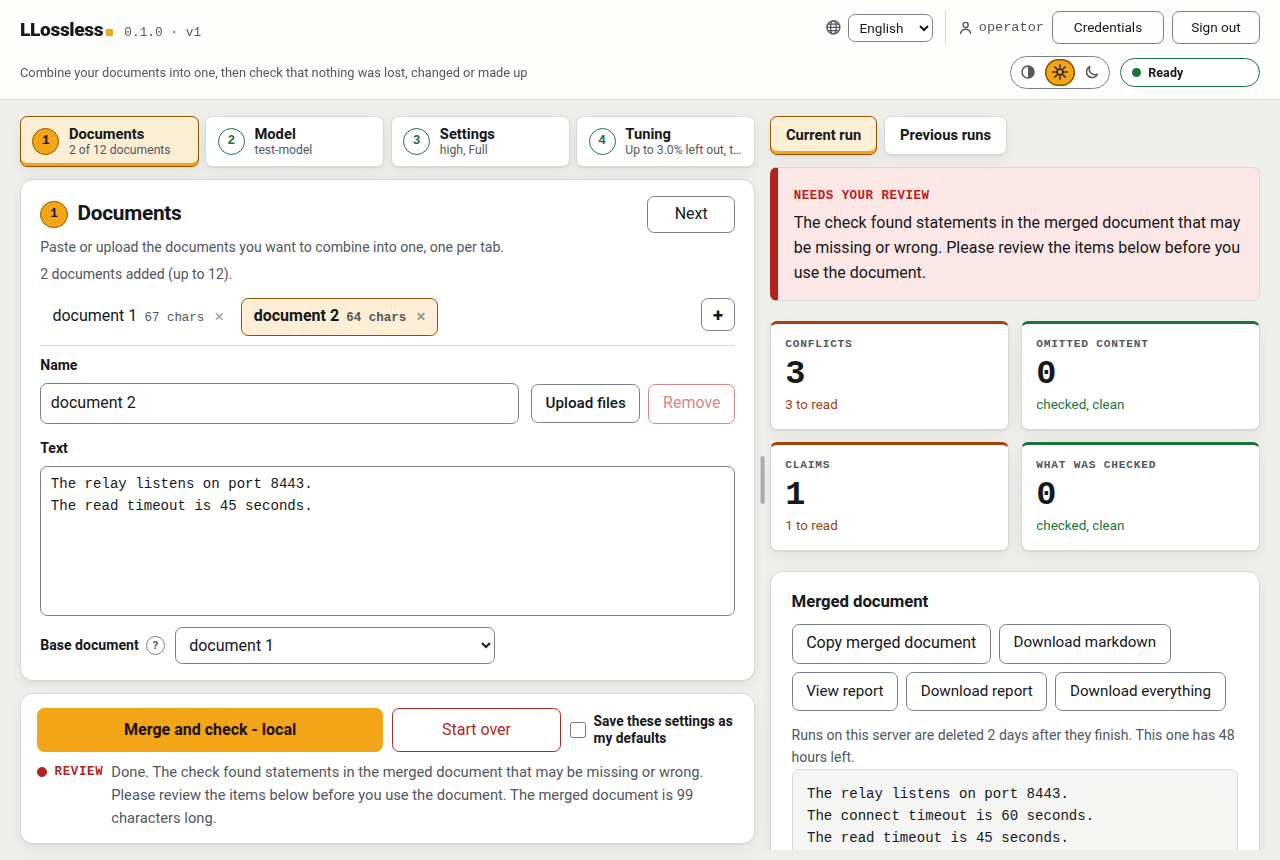
\includegraphics[width=\linewidth]{../docs/img/web-ui-light.png}
\caption{The web interface after a run with findings: the documents on the left, and on the right the findings, the checks that ran and the merged document with its downloads. The answers in this screenshot came from a scripted test endpoint, not from a real model.}
\label{fig:webui}
\floatfoot
\end{figure}

\paragraph{Rules that do not depend on the level.} In a merge the tool made, numbers, links, file paths, version strings and code must arrive character for character at every level. A changed one is a finding.

What a merge states from outside the documents has three possible outcomes at \texttt{open}, and the tool treats them differently:
\begin{points}
\item \emph{Declared, and the documents say nothing on the matter.} The statement is listed in the report for review. It is not a finding.
\item \emph{Declared, and it contradicts a source.} This is a correction. It is listed in the report, and it is still a finding that fails the run. The tool cannot tell a correction from an error, because the documents are the only reference it has.
\item \emph{Not declared.} The statement is reported as invented.
\end{points}

\noindent One run of the benchmark shows the second case. A source of the Voyager set says that the names of some newly found moons are ``obvious allusions to Goethe''. That is one of the errors I planted. At \texttt{open} the model wrote ``allusions to Shakespeare and Alexander Pope'' and declared the change. Shakespeare and Alexander Pope is the correct fact and Goethe is the error I planted, so the model put the planted error right. The report still lists the statement among those added from outside the documents. It also reports that the merge contradicts its source, and the run ends with exit code 1, because the tool cannot tell a correction from a contradiction. A person has to confirm the correction.

\paragraph{What comes back.} A run returns a report and an exit code. The report is in Markdown, and on request the same report comes as JSON or as a self-contained HTML page. It opens with a summary of what was found. Then come the findings. A \emph{finding} is an entry that names one problem. Each finding of the judged checks names the claim, its file and line, and the evidence quoted. Every claim that was drawn from the documents is listed with what became of it. A block at the end records which model answered in each role, the settings, the cost and whether document content left the machine.

The exit code tells a script how the run went:

\begin{center}\small
\begin{tabular}{@{}lp{0.80\linewidth}@{}}
\toprule
Code & Meaning \\
\midrule
0 & Nothing was found. \\
1 & There is a problem in the merged document. The runbook merge of the opening story ended this way. \\
2 & The run could not finish, or could not check everything. I call such a run \emph{inconclusive}. \\
3 & Milder than 1: the merged document passed every check, but the merge's records are wrong or incomplete. Example: a record says a sentence was replaced, and the sentence is still in the merge unchanged. Or the sources head the same section differently, and the merge kept one heading and wrote no record for the other. \\
\bottomrule
\end{tabular}
\end{center}

\noindent When more than one applies, the run returns the most serious: 2 before 1, and 1 before 3. An inconclusive run is not a pass. A run that checked nine claims of twelve has not shown the merge clean, so any unfinished part makes the whole run inconclusive.

\section{How the checks work}
\label{sec:system}

This section explains what happens between the merge and the report. The checks described here are the guardrails of Section~\ref{sec:problem}, taken one at a time.

A merge can go wrong in three ways: it can drop something, change something, or invent something. A checker that is itself a language model can go wrong in the same three ways. So what can be decided by comparing strings is decided that way, and a model is asked only about meaning. That gives two families of checks. The \emph{mechanical checks} are a program. A reader can verify any of their findings with a text editor. The \emph{judged checks} rest on a model, the judge. The tool keeps the two apart in the report, and Section~\ref{sec:trust} leans on that split. Figure~\ref{fig:pipeline} shows the steps of a run in order.

% Figure: the pipeline at a glance, merge then verify. Placed at the start of
% Section 3. Blue boxes are a program, orange boxes a model. The exit codes are
% the tool's design constants, stated in Section 2.
\begin{figure}[H]
\centering
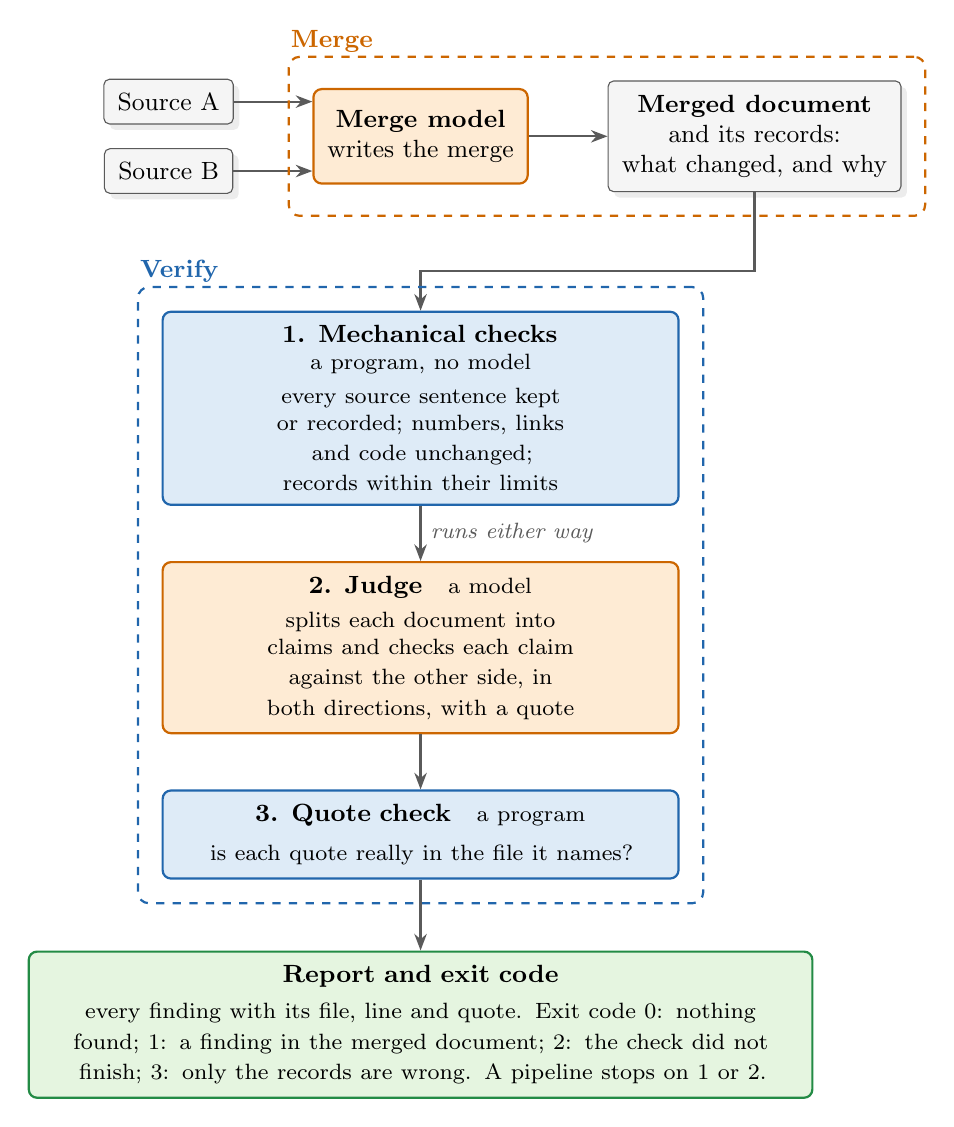
\begin{tikzpicture}[node distance=8mm and 9mm]
  \node[doc] (a) {Source A};
  \node[doc, below=3mm of a] (b) {Source B};
  \coordinate (ab) at ($(a.east)!0.5!(b.east)$);
  \node[model, right=10mm of ab, minimum height=12mm] (merge)
       {\textbf{Merge model}\\writes the merge};
  \node[doc, right=10mm of merge, minimum height=12mm] (out)
       {\textbf{Merged document}\\and its records:\\what changed, and why};
  \draw[flow] (a.east) -- (a.east -| merge.west);
  \draw[flow] (b.east) -- (b.east -| merge.west);
  \draw[flow] (merge) -- (out);

  \node[prog, below=16mm of merge, text width=62mm] (mech)
       {\textbf{1. Mechanical checks}\quad\footnotesize a program, no model\\[3pt]
        every source sentence kept or recorded; numbers, links\\and code unchanged; records within their limits};
  \node[model, below=7mm of mech, text width=62mm] (judge)
       {\textbf{2. Judge}\quad\footnotesize a model\\[3pt]
        splits each document into claims and checks each claim\\
        against the other side, in both directions, with a quote};
  \node[prog, below=7mm of judge, text width=62mm] (quote)
       {\textbf{3. Quote check}\quad\footnotesize a program\\[3pt]
        is each quote really in the file it names?};
  \node[good, below=9mm of quote, text width=96mm] (report)
       {\textbf{Report and exit code}\\[2pt]\footnotesize
        every finding with its file, line and quote. Exit code 0: nothing found;
        1: a finding in the merged document; 2: the check did not finish;
        3: only the records are wrong. A pipeline stops on 1 or 2.};
  \draw[flow] (out.south) |- ($(mech.north)+(0,5mm)$) -- (mech.north);
  \node[draw=modelorange, dashed, thick, rounded corners=4pt, inner sep=3mm,
        fit=(merge) (out)] (mergebox) {};
  \node[font=\small\bfseries, text=modelorange, anchor=south west, inner sep=1pt]
    at (mergebox.north west) {Merge};
  \node[draw=progblue, dashed, thick, rounded corners=4pt, inner sep=3mm,
        fit=(mech) (judge) (quote)] (verifybox) {};
  \node[font=\small\bfseries, text=progblue, anchor=south west, inner sep=1pt]
    at (verifybox.north west) {Verify};
  \draw[flow] (mech) -- node[lbl, right] {runs either way} (judge);
  \draw[flow] (judge) -- (quote);
  \draw[flow] (quote) -- (report);
\end{tikzpicture}
\caption{What happens in one run, in order: the merge, then its verification.
\texttt{llossless merge} does both; \texttt{llossless verify} does only the second, on a
merge made elsewhere. Blue boxes are a program, which compares text and cannot invent
anything. Orange boxes are a model. A model writes the merge, and a model
judges what only meaning can settle, but every quote it gives as evidence is checked by
a program.}
\label{fig:pipeline}
\floatfoot
\end{figure}


\subsection{What a program can settle}

\paragraph{Segments.} A program first cuts every document into \emph{segments}. A segment is a sentence, or one of the other units a document is built from: a heading, a list item, a table row, a block of code set off by fences. The field crew's sentence ``Escalate E2 to the workshop after 2 failed attempts.'' is one segment. A segment also ends where a line of the file ends on a comma or another punctuation mark. So the support desk's sentence ``If the field crew have already tried 3 times, raise it to the workshop instead.'' is two segments, cut after the comma, where its line ends. Sources and merge are cut the same way, so the program can look for a source segment in the merge without asking a model.

\paragraph{Protected values.} Some parts of a segment must never change: numbers, version strings, inline code, file paths, links and URLs. I call them protected values. A fenced code block is protected byte for byte. A merge may rewrite the sentence around a command that is written as inline code, but not the command. It may not re-indent a fenced YAML block.

\paragraph{Records.} The merge model returns the merged document and one record for every source segment it did not copy word for word. A record names the segment, says what happened to it, and gives a reason. There are six kinds:

\begin{center}\small
\begin{tabular}{@{}lp{0.74\linewidth}@{}}
\toprule
Kind of record & What the merge says happened to the segment \\
\midrule
reworded & The same content is in the merge in other words. \\
superseded & Another source's version of this content was used instead. \\
subsumed & The content is inside a broader statement of the merge. \\
duplicate & Another segment already says this. \\
combined & This segment and another were joined into a statement that neither makes alone. \\
dropped & The content is not in the merge, and nothing replaces it. \\
\bottomrule
\end{tabular}
\end{center}

\noindent In the opening story the record for the support desk's sentence is of the kind \emph{\ccnum{lineup.story.disposition}}, with the reason ``\ccnum{lineup.story.reason}'' A record of the kinds reworded, superseded, subsumed or duplicate also names a \emph{replacement}: the text in the merge that is said to carry the content now.

\paragraph{The rule that makes loss checkable.} Whether a merge lost anything is a question no program can answer by itself. A sentence that is missing from the merge may have been reworded, folded into another sentence, or dropped. The records turn this into a question a program can answer. Every source segment must be in the merge word for word, or it must have a record. For a segment that is not there word for word, the program looks further, by similarity and by the run of its words (Appendix~\ref{sec:checks}). If it finds the segment in altered form, the segment counts as reworded, and a reworded segment with no record is a finding. If it does not find it, the segment is missing. A segment that is missing and has no record is a silent loss, and the mechanical checks report it. Figure~\ref{fig:sentence} draws the whole rule.

The program also checks the records against the text, as far as a comparison of text can. The replacement that a record names must be in the merge. And a record must not describe a change that did not happen. A record may say that a segment was subsumed or superseded while the merge still carries that segment unchanged. No content is lost then, but the merge's account of its own work is false. Exit code 3 is for this case (Section~\ref{sec:false-departure}), and for an \emph{untaken heading}: a source heading that the merge did not take and wrote no record for, while its section is in the merge under another heading.

\paragraph{Two limits on records.} A model could use records to excuse any loss, so two rules limit them. The first is the \emph{loss budget}. A merge may declare segments dropped, with records of the kind dropped, but not more than \ccnum{tool.loss_budget_percent}\% of the source segments it was given. That figure is the default, and the user can change it with the option \texttt{-{}-loss-budget}. The second limits a replacement. One replacement may stand in for at most \ccnum{tool.fan_in} missing segments. A single sentence that claims to carry many detailed ones has dropped them. Section~\ref{sec:declared-blindspot} says where the second rule came from and what it still misses.

% Figure: what becomes of one source sentence. Placed in Section 3, after the
% rule that makes loss checkable. Every question in it is answered by a program.
\begin{figure}[H]
\centering
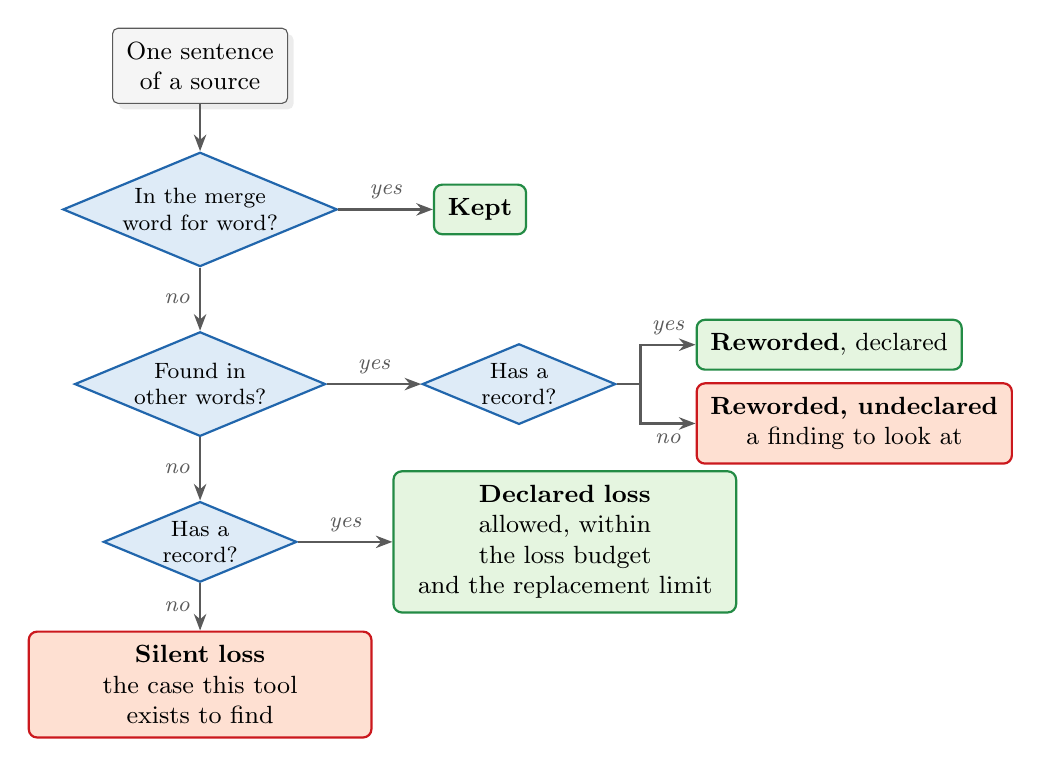
\begin{tikzpicture}[node distance=6mm and 9mm]
  \node[doc] (s) {One sentence\\of a source};
  \node[ask, below=6mm of s] (q1) {In the merge\\word for word?};
  \node[good, right=12mm of q1] (kept) {\textbf{Kept}};
  \node[ask, below=8mm of q1] (q2) {Found in\\other words?};
  \node[ask, right=12mm of q2] (r1) {Has a\\record?};
  \node[good, right=10mm of r1, yshift=5mm] (rw) {\textbf{Reworded}, declared};
  \node[bad, right=10mm of r1, yshift=-5mm] (rwu) {\textbf{Reworded, undeclared}\\a finding to look at};
  \node[ask, below=8mm of q2] (q3) {Has a\\record?};
  \node[good, right=12mm of q3, text width=40mm] (dec)
       {\textbf{Declared loss}\\allowed, within the loss budget\\and the replacement limit};
  \node[bad, below=6mm of q3, text width=40mm] (sil)
       {\textbf{Silent loss}\\the case this tool exists to find};
  \draw[flow] (s) -- (q1);
  \draw[flow] (q1) -- node[lbl, above] {yes} (kept);
  \draw[flow] (q1) -- node[lbl, left] {no} (q2);
  \draw[flow] (q2) -- node[lbl, above] {yes} (r1);
  \draw[flow] (r1.east) -- ++(3mm,0) |- node[lbl, pos=0.75, above] {yes} (rw.west);
  \draw[flow] (r1.east) -- ++(3mm,0) |- node[lbl, pos=0.75, below] {no} (rwu.west);
  \draw[flow] (q2) -- node[lbl, left] {no} (q3);
  \draw[flow] (q3) -- node[lbl, above] {yes} (dec);
  \draw[flow] (q3) -- node[lbl, left] {no} (sil);
\end{tikzpicture}
\caption{What becomes of one sentence of a source. Every question here is answered by a
program. Green outcomes are allowed. Red ones are reported, and a silent loss is the case
the tool exists to find. Because the program compares text and not meaning, it can call a
sentence missing that the merge kept in very different words, so a silent loss is a place
to look and not proof.}
\label{fig:sentence}
\floatfoot
\end{figure}


\paragraph{How the mechanical checks decide.} There are \ccnum{tool.checks} mechanical checks, built from four operations. A search looks for one text in another, character for character or word for word. Regular expressions cut documents into segments and find protected values. A similarity score with a fixed cut-off helps to tell reworded from missing. The rest is counting. The code is plain Python with its standard library, \texttt{re} for the patterns and \texttt{difflib} for the score. No model is asked, so the same input gives the same findings. Appendix~\ref{sec:checks} lists the checks one by one, says how a segment is looked for, and gives the patterns for protected values.
\paragraph{What the program reports on two real merges.} Here are two merges of the runbooks from Section~\ref{sec:problem}, taken from the benchmark. The program caught both, and it judged them differently.

\bigskip\noindent\textbf{Example 1: a near-duplicate dropped.}

\begin{center}\small
\vspace{2pt}
\begin{tabular}{@{}lp{0.74\linewidth}@{}}
\toprule
Field crew & Report E4 to the electrical contractor the same day. \\
Support desk & Raise an E4 to the electrical contractor the same day. \\
Reference merge & Keeps both sentences. \\
Merge & By \texttt{\ccnum{lineup.haiku-4.5-sub.name}}: keeps the field crew's sentence, drops the support desk's, writes no record. \\
Program & \texttt{is reworded in the merge and no disposition record explains it} \\
\bottomrule
\end{tabular}
\end{center}
\vspace{4pt}

\noindent The program looked for the support desk's sentence and found the field crew's, which is nearly the same. So it reports the sentence as reworded without a record. That is listed for a person to look at, but it is not a silent loss. Both readings of the audit found the content still in the merge.

\bigskip\noindent\textbf{Example 2: a number dropped.}

\begin{center}\small
\vspace{2pt}
\begin{tabular}{@{}lp{0.74\linewidth}@{}}
\toprule
Field crew & Escalate E2 to the workshop after \ccnum{lineup.story.a_count} failed attempts. \\
Support desk & If the field crew have already tried \ccnum{lineup.story.b_count} times, raise it to the workshop instead. \\
Reference merge & Keeps \ccnum{lineup.story.a_count}. Its record says that the support desk's sentence was superseded by the field crew's. \\
Merge & By \texttt{\ccnum{lineup.sonnet-5-api.name}}: keeps \ccnum{lineup.story.a_count}, drops \ccnum{lineup.story.b_count}, and writes the record ``Attempt-count disagreement resolved to the base's value of 2.'' \\
Program & \texttt{numeric \textquotesingle{}3\textquotesingle{} (times) does not survive into the merge unchanged} \\
\bottomrule
\end{tabular}
\end{center}
\vspace{4pt}

\noindent The model made the reference merge's choice and declared it, but a number is a protected value. A record excuses a missing number only when the replacement it names is the wording of a source sentence (Appendix~\ref{sec:checks}). The reference merge's record names the field crew's sentence as written. This record names it joined to the one after it, which no source has in that form. So the program reports the \ccnum{lineup.story.b_count} as missing.

\paragraph{What the mechanical checks cannot see.} When a record names a replacement, the program checks that the replacement is in the merge, not that it says what the missing sentence said. The merge of Section~\ref{sec:problem} is an example. Its record names the field crew's ``Escalate E2 to the workshop after \ccnum{lineup.story.a_count} failed attempts.'' as the replacement for the support desk's sentence with \ccnum{lineup.story.b_count}. Unlike the record in the second example above, it names a sentence that stands in the merge exactly as a source wrote it, so the mechanical checks accept the record. That the two numbers disagree is a question of meaning, and it was the judge that reported it. Such questions go to the judge (Section~\ref{sec:judged}). Section~\ref{sec:declared-blindspot} shows how far a merge could push this.

\subsection{What needs a judge}
\label{sec:judged}

Whether ``refund at the time of the call'' survived in a sentence that says ``refund immediately'' is a question about meaning. For such questions the tool asks a model, the judge.

\paragraph{Claims.} The judge first splits each document into \emph{claims}, short statements of one fact each, with the line each comes from. In the literature these are called atomic claims. Segments and claims are different things. A segment is a piece of the text as it stands, cut by a program. A claim is a statement of what the text says, written by a model. One segment can hold several claims. The field crew's runbook has the sentence ``E2 is a mechanical fault and E4 is an electrical one, and they are escalated differently.'' From it the judge drew three claims: ``E2 is a mechanical fault.'', ``E4 is an electrical fault.'' and ``E2 and E4 are escalated differently.''

\paragraph{Both directions.} The judge then compares each claim with the other side and gives a verdict. Every source claim is compared with the merge. Every merge claim is compared with the sources. Three verdicts are findings:
\begin{points}
\item A source claim that is missing from the merge was \emph{dropped}.
\item A merge claim that is missing from the sources was \emph{invented}.
\item A claim that the other side states differently is \emph{contradicted}.
\end{points}

\noindent Checking both directions is the default. The tool calls it the verification depth \texttt{\ccnum{tool.default_depth}}. A cheaper depth, \texttt{coverage}, compares only the source claims with the merge. It can find what was dropped, but it cannot find what was invented. Section~\ref{sec:depth} measures the difference.

\paragraph{A verdict must quote its evidence.} A judge can be confidently wrong. So a verdict that rests on what the other side says must quote it. The quote must be \emph{grounded}: the tool looks for the quoted text in the file the judge named, and it has to be there. This is one of the two findings about the count in the opening story:

\begin{quote}\small
\texttt{source\_b.md:15} says: If the field crew have already tried 3 times on an E2 fault, the fault is raised to the workshop instead.\\[3pt]
\texttt{merged.md} says: \textquotesingle{}Escalate E2 to the workshop after 2 failed attempts.\textquotesingle{} (grounded)\\[3pt]
judged against: \texttt{merged.md}\\[3pt]
why this was read as a contradiction: The reference text sets the escalation threshold at 2 failed attempts, not 3.
\end{quote}

\noindent These are the lines of the report, as it prints them. The first is a claim that the judge drew from the support desk's runbook, in the judge's own words, with its file and line. The second is the quote that the judge gave as evidence. ``Grounded'' means that the tool found that quote, word for word, in the merged document. The judge calls the document it checks against ``the reference text'', and here that is the merged document. A person can check the finding by opening both files at the places named. A quote that is in none of the files is reported as a transcription error.

\paragraph{When the judge did not finish.} Two cases make a run inconclusive, with exit code 2. In the first, claims were graded and not one quote could be grounded, so nothing was measured. In the second, the judge failed to grade a claim even after a fixed number of retries. The claim is then listed as not graded. This happens when the judge's answer for that claim breaks the required format, for example by naming a claim it was not asked about, and the judge is told what is wrong and still gets it wrong on every retry.

\subsection{Running against real endpoints}

Two practical matters decide whether the checks can be relied on from day to day. One is whether a model's answer arrives in a form a program can read. The other is whether the tool's own tests can run without a model.

\paragraph{Answers a program can read.} Every model answer is JSON that must match a schema, which is a formal description of the fields the answer must have. Endpoints differ in how firmly they can be held to a schema. The tool knows three ways and uses the strongest one the endpoint supports. In the strongest, the endpoint enforces the schema itself. In the second, the schema is the parameter list of a function the model must call. In the weakest, the schema is only described in the prompt. The report records which was used.

One lesson came from this. A schema with a single optional field made one vendor's strongest mode refuse the schema. The tool then fell back to the weakest way, and no error appeared anywhere. Since then no schema the tool sends has an optional field, and a test holds the merge schema to that at every fidelity level.

\paragraph{Tests without a model.} The test suite needs no model. The model answers its figures depend on were recorded from real models and are replayed with no network. Each recorded answer is stored under a digest of the request that produced it. So when a prompt changes, the request changes, and the old recordings no longer match. The figures that depended on them are then reported as \emph{unmeasured}, not as passes.

% The measurements come before the section on how the figures are kept honest:
% a reader has to have seen a figure before being told why it can be checked.
% The files keep their names, because the number check names sections by file.
% A REGISTERED RESULT SECTION. Numerals only through \ccnum, including the ones
% that look like names: a model identifier is read out of a record's provenance
% or out of a registration, not typed.
\section{What it measured: a dated snapshot}
\label{sec:findings}

This section reports what current models did when they merged the same documents under the tool's checks, on one date. The main question is which models lose content without saying so, and which merge best. Smaller measurements follow: which model fixes errors in its sources, which notices a bad merge, whether the route matters, what the cheaper check misses, and what the local models I tried first did.

\paragraph{A snapshot, not a leaderboard.} Models changed faster than I could measure them (Section~\ref{sec:lessons}). So the figures describe one fixed set of models, measured in one session that began on \ccnum{lineup.from} and ended shortly after midnight UTC on \ccnum{lineup.to}, with one fixed version of the tool.

\paragraph{Written down before the run.} The benchmark was \emph{registered}: its question, its models, its settings and its rules were written into a file in the repository, in the directory \texttt{\ccnum{reg.2026-09-27-lineup.path}}, before the first model call. A later correction goes below the original text as a dated \emph{amendment}. The file carries \ccnum{reg.2026-09-27-lineup.amendments} amendments. The first and the second were written before the calls they govern. The third and the fourth are of another kind. I wrote both on \ccnum{lineup.amended.date}, after every call and with the results known, and Section~\ref{sec:audit} is about them. The fifth and the sixth, of \ccnum{lineup.amendments.last_date}, correct the reference merges of the runbook pair and the loading-dock pair. Each had kept a value that a merge at the default level is told to choose away or remove, the support desk's count and the hours of a retired phone line, in a sentence of its own that is in neither source. Only the amended scoring's deviations on those pairs move, and the order does not.

\subsection{What was run, and how it was scored}

\paragraph{The models and the configurations.} The benchmark covers models of the vendors Anthropic and OpenAI. Anthropic's are \texttt{\ccnum{lineup.opus-5.5-api.model}}, \texttt{\ccnum{lineup.sonnet-5-api.model}} and \texttt{\ccnum{lineup.haiku-4.5-api.model}}, which I call Opus, Sonnet and Haiku. Opus is the \ccnum{lineup.story.row_label} of the opening story, and the merge told there is from the configuration \texttt{\ccnum{lineup.opus-5.5-api.name}}. OpenAI's are \texttt{\ccnum{lineup.gpt-6-sol-api.model}} and \texttt{\ccnum{lineup.gpt-6-luna-api.model}}, which I call the GPT models. All of them are hosted models. Opus, Sonnet and \texttt{\ccnum{lineup.gpt-6-sol-api.model}} are \emph{frontier models}. Haiku and \texttt{\ccnum{lineup.gpt-6-luna-api.model}} are the small, cheaper model of each vendor. Take the list price of output from \texttt{\ccnum{lineup.gpt-6-luna-api.model}}, the cheapest, as the unit. Output from Haiku then costs \ccnum{lineup.haiku-4.5-api.list_output_multiple} times as much, from Sonnet \ccnum{lineup.sonnet-5-api.list_output_multiple} times, from \texttt{\ccnum{lineup.gpt-6-sol-api.model}} \ccnum{lineup.gpt-6-sol-api.list_output_multiple} times, and from Opus \ccnum{lineup.opus-5.5-api.list_output_multiple} times.

The Anthropic models ran on the API route and on the subscription route, and the GPT models on the API route only. That gives \ccnum{lineup.rows} configurations. The name of a configuration joins the model and the route: \texttt{\ccnum{lineup.opus-5.5-api.name}} is Opus through the API, and \texttt{\ccnum{lineup.opus-5.5-sub.name}} is Opus through the subscription. In every run the configuration's model filled all the roles: it wrote the merge, and it was the judge of that merge. That is how I set the benchmark up, and it is not a limit of the tool (Section~\ref{sec:usage}). Every call to the judge is a new request with a fresh context, so the judge sees the documents and the claims and nothing of the conversation in which the merge was written.

Another Anthropic model, Fable (\texttt{\ccnum{lineup.side.fable-sub.model}}), ran through the subscription on a few documents only. I chose those documents after the results of Opus were in and before any call to Fable, as the second amendment records. Fable appears once, in Table~\ref{tab:planted}. \ccnum{lineup.unmeasured.name} was to run beside the others and has no figure: its vendor's free tier refused every call, and I did not run it on a paid tier, for reasons of budget.

\paragraph{The test material.} Every configuration ran the same files.
\begin{points}
\item \emph{Merging.} The \ccnum{lineup.pairs} pairs, merged at the default level \texttt{high}. A pair is the same procedure written down twice, as separate teams might write it for different readers. The bike-share runbooks are one pair. Others are about visitor badges, a payroll deadline and a freezer alarm. Every pair has a reference merge, with the records that belong to it. The files are in \texttt{tests/pairs/}.
\item \emph{Fixing errors.} The Voyager set and the seed-phrase set, whose sources carry planted errors, and the Mah-Jongg set, which carries none. These were merged at \texttt{open}, the level that lets a merge correct a source.
\item \emph{Detection.} The \ccnum{lineup.fixtures} test cases that I had registered for this purpose (Section~\ref{sec:detection}).
\end{points}

\paragraph{How often each ran.} Most pairs ran once on each configuration. The Voyager set and the seed-phrase set ran \ccnum{lineup.opus-5.5-sub.spread.rate_limits.draws} times on every configuration, and so did the pairs \texttt{badge\_access}, \texttt{trace\_names} and \texttt{rate\_limits}, except on \texttt{\ccnum{lineup.sonnet-5-api.name}} and \texttt{\ccnum{lineup.haiku-4.5-api.name}}. There the first amendment took those repeats out, to keep the cost of the Anthropic API under the cap I had set. I call these the repeated pairs. A model does not give the same answer twice, and the repeats show how far a figure moves from one run to the next. No answer was shared between runs, except that a run started again after a failure reused the answers its own earlier attempt had received.

\paragraph{The rule for ordering.} The rule is not a combined score. First, a configuration that lost content with no record on the first run of any pair is disqualified. The audit decides that, not the program's count. Then the others are ordered by their deviations from the reference merges, fewest first. Configurations with the same number share a place, unless all of them are billed at list price. Then the lower cost decides. A weighted score would let a cheap model buy back lost facts with its price, which is the trade this tool exists to refuse. The rule encodes my requirement, as little loss as possible, and a user who wants the lowest price would order the table differently. Because most of it rests on a single run, I call the result an order and not a ranking.

In total the benchmark cost \$\ccnum{lineup.spend.anthropic} at list price for the Anthropic API configurations and \$\ccnum{lineup.spend.openai} for the OpenAI ones. The subscription configurations came to \$\ccnum{lineup.spend.subscription} API-equivalent, which is not a bill. The earlier measurements on rented GPUs (Section~\ref{sec:study}) cost several times as much.

\paragraph{What was not the same for everyone.} The route differed. The judge graded \ccnum{tool.verify_batch_http} claims per call over the API and \ccnum{tool.verify_batch_command} through the command-line program. Only the OpenAI configurations sent a seed, the setting that makes a model's answers more repeatable. And the reasoning effort, a vendor setting for how much a model reasons before it answers, differed.

\subsection{Who loses content, and who merges best}
\label{sec:lineup}

On the first runs the program counted a silent loss for \ccnum{lineup.flagged_rows} of the \ccnum{lineup.rows} configurations (Table~\ref{tab:lineup}). A count is a flag, so the audit read the segments: \ccnum{lineup.audit.both.first.cases} on the first runs, each of them twice. They were the \ccnum{lineup.audit.first.cases} that the registered scoring had counted as silent loss and the \ccnum{lineup.audit.reworded.cases} that the program had passed as reworded although no record named them. In \ccnum{lineup.audit.both.first.lost} of them it found content gone, wholly or in part, with no record. Those \ccnum{lineup.audit.both.first.lost} are in the merges of \ccnum{lineup.disqualified} configurations, and the rule disqualifies them: the Haiku configurations, \texttt{\ccnum{lineup.haiku-4.5-sub.name}} and \texttt{\ccnum{lineup.haiku-4.5-api.name}}, and \texttt{\ccnum{lineup.gpt-6-luna-api.name}}. Each is the small model of its vendor, and no configuration of a frontier model is among them. Each Haiku configuration lost content in more than one place. \texttt{\ccnum{lineup.gpt-6-luna-api.name}} is disqualified for one sentence: it lost its opening condition, with no record, and both readings call the case borderline. I ruled that it disqualifies, and Section~\ref{sec:audit} quotes it. \texttt{\ccnum{lineup.sonnet-5-sub.name}} is the one configuration with a counted silent loss that is not disqualified. The audit read \ccnum{lineup.sonnet-5-sub.audit.cases} of its segments and found every one of them in the merge.

Of the \ccnum{lineup.survivors} configurations that are not disqualified, \texttt{\ccnum{lineup.gpt-6-sol-api.name}} comes first under the rule. It has the fewest deviations of any configuration, \ccnum{lineup.gpt-6-sol-api.dev_per_pair} a pair, and no counted silent loss on a first run. \texttt{\ccnum{lineup.opus-5.5-sub.name}} and \texttt{\ccnum{lineup.sonnet-5-sub.name}} have \ccnum{lineup.opus-5.5-sub.dev_per_pair} deviations a pair each and share the second place. Cost does not decide between them, because their costs are API-equivalents and not list prices. \texttt{\ccnum{lineup.opus-5.5-api.name}} and \texttt{\ccnum{lineup.sonnet-5-api.name}} come last, at \ccnum{lineup.opus-5.5-api.dev_per_pair} and \ccnum{lineup.sonnet-5-api.dev_per_pair}. \texttt{\ccnum{lineup.sonnet-5-api.name}} is also the slowest API configuration. Figure~\ref{fig:cost} sets the deviations against the cost of a merge.

\paragraph{The baselines.} The rows at the foot of the table are texts made by a script from the sources of a pair and scored like a merge. \emph{Sources concatenated} is both sources pasted one after the other. \emph{Mechanical union} is one source followed by every paragraph of the other that the first does not already contain. \emph{Base only} is the base source alone. The mechanical union loses nothing and has \ccnum{lineup.floor.union.dev_per_pair} deviations a pair. That is the figure a model has to beat to have done more than a script. Every configuration beats it: each has fewer deviations than the mechanical union on the pairs it finished. Concatenating the sources loses nothing either, which is why a benchmark that scores only whether the sources survived cannot tell a model from a script. Base only loses whatever only the other source says. The program counts \ccnum{lineup.floor.base_only.silent} segments over the \ccnum{lineup.pairs} pairs as silent loss, and \ccnum{lineup.floor.base_only.untaken} headings as untaken. Its deviation figure still looks ordinary, because a reference merge replaces most segments of the second source with a record for each and the deviation count does not look at records. That is why the order needs both measures.

% Figure: price against merge quality. Placed in Section 4.2. Every plotted
% value is a generated figure. The axis limits and the shaded zone are layout,
% and check_numbers.py holds the data to them (`_cost_figure`), so a point that
% leaves them fails the build.
\newcommand{\costpoint}[4]{% row, vendor colour, mark, where the label goes
  \addplot[only marks, mark=#3, mark size=3.2pt, color=#2, line width=1pt]
    coordinates {(\ccnum{lineup.#1.usd},\ccnum{lineup.#1.dev_per_pair})};
  \node[font=\scriptsize\ttfamily, color=#2, #4]
    at (axis cs:\ccnum{lineup.#1.usd},\ccnum{lineup.#1.dev_per_pair}) {\ccnum{lineup.#1.name}};
}
\begin{figure}[H]
\centering
\begin{tikzpicture}
\begin{axis}[
  width=0.92\linewidth, height=8cm,
  xmode=log, log basis x=10,
  xmin=0.008, xmax=1.4, ymin=3.4, ymax=8.4,
  xtick={0.01,0.03,0.1,0.3,1}, xticklabels={\$0.01,\$0.03,\$0.10,\$0.30,\$1.00},
  xlabel={Cost per merge (log scale)}, ylabel={Deviations per pair},
  grid=major, grid style={draw=black!8},
  axis line style={draw=docgrey}, tick label style={font=\footnotesize},
  label style={font=\small},
  clip=false,
]
  % The zone reaches a little beyond the configuration that is cheapest and closest, by the
  % factor and the margin below; check_numbers.py requires that no other row falls in it.
  \fill[goodfill, opacity=0.55] (axis cs:0.008,3.4) rectangle
    (axis cs:{\ccnum{lineup.gpt-6-sol-api.usd}*1.3},{\ccnum{lineup.gpt-6-sol-api.dev_per_pair}+0.7});
  \node[font=\scriptsize\itshape, color=goodgreen, anchor=south west]
    at (axis cs:0.0085,3.45) {cheap and close to the reference};
  \draw[dashed, thick, color=badred] (axis cs:0.008,\ccnum{lineup.floor.union.dev_per_pair})
    -- (axis cs:1.4,\ccnum{lineup.floor.union.dev_per_pair});
  \node[font=\scriptsize, color=badred, anchor=south east]
    at (axis cs:1.35,\ccnum{lineup.floor.union.dev_per_pair})
    {a script pasting the documents together};
  \costpoint{gpt-6-sol-api}{openai}{*}{anchor=west, xshift=4pt}
  \costpoint{gpt-6-luna-api}{openai}{o}{anchor=west, xshift=4pt}
  \costpoint{opus-5.5-api}{anthropic}{*}{anchor=north, yshift=-6pt}
  \costpoint{opus-5.5-sub}{anthropic}{square*}{anchor=west, xshift=5pt, yshift=-3pt}
  \costpoint{sonnet-5-api}{anthropic}{*}{anchor=south east, xshift=-3pt, yshift=6pt}
  \costpoint{sonnet-5-sub}{anthropic}{square*}{anchor=east, xshift=-5pt}
  \costpoint{haiku-4.5-api}{anthropic}{o}{anchor=west, xshift=4pt}
  \costpoint{haiku-4.5-sub}{anthropic}{square}{anchor=west, xshift=4pt}
\end{axis}
\end{tikzpicture}
\caption{Price against merge quality on the \ccnum{lineup.pairs} pairs: lower is closer
to the reference merges. Orange is Anthropic, teal OpenAI. Circles are the vendor's API,
squares its command-line program under a subscription, whose cost is the API-equivalent
and not a bill. Hollow markers are disqualified for lost content. The dashed line is a
script with no model; every configuration is below it.}
\label{fig:cost}
\floatfoot
\end{figure}


\paragraph{What the registered scoring said.} Under the scoring as registered, the program's count disqualified, and it disqualified \ccnum{lineup.registered.disqualified} of the \ccnum{lineup.rows} configurations: the Haiku configurations, \texttt{\ccnum{lineup.gpt-6-luna-api.name}}, \texttt{\ccnum{lineup.opus-5.5-api.name}} and \texttt{\ccnum{lineup.sonnet-5-sub.name}}. But the registered count was mostly not lost content: the reading found content gone in \ccnum{lineup.audit.first.lost} of the \ccnum{lineup.audit.first.cases} segments it counted on first runs, and the count of \ccnum{lineup.registered.opus-5.5-api.silent} that disqualified \texttt{\ccnum{lineup.opus-5.5-api.name}} was \ccnum{lineup.opus-5.5-api.untaken} untaken headings. The registered scoring also found that one model did no better than a script: \texttt{\ccnum{lineup.sonnet-5-api.name}} had \ccnum{lineup.registered.sonnet-5-api.dev_per_pair} deviations a pair against \ccnum{lineup.registered.floor.union.dev_per_pair} for the mechanical union, where the amended scoring has \ccnum{lineup.sonnet-5-api.dev_per_pair} against \ccnum{lineup.floor.union.dev_per_pair}. \texttt{\ccnum{lineup.gpt-6-sol-api.name}} is first under both scorings. Every figure of the registered scoring is in \texttt{figures.md} in the benchmark's directory.

\begin{table}[H]
\centering\small
\begin{tabular}{@{}llrrrrrrr@{}}
\toprule
 & & Pairs & Silent & Untaken & Lost, by & Deviations & Cost & Seconds \\
Configuration & Order & done & loss & headings & reading & /pair & /merge & /merge \\
\midrule
\texttt{\ccnum{lineup.gpt-6-sol-api.name}} & \ccnum{lineup.gpt-6-sol-api.place} & \ccnum{lineup.gpt-6-sol-api.pairs_completed}/\ccnum{lineup.pairs} & \ccnum{lineup.gpt-6-sol-api.silent} & \ccnum{lineup.gpt-6-sol-api.untaken} & \ccnum{lineup.gpt-6-sol-api.audit.found} & \ccnum{lineup.gpt-6-sol-api.dev_per_pair} & \$\ccnum{lineup.gpt-6-sol-api.usd} & \ccnum{lineup.gpt-6-sol-api.seconds} \\
\texttt{\ccnum{lineup.opus-5.5-sub.name}} & \ccnum{lineup.opus-5.5-sub.place} & \ccnum{lineup.opus-5.5-sub.pairs_completed}/\ccnum{lineup.pairs} & \ccnum{lineup.opus-5.5-sub.silent} & \ccnum{lineup.opus-5.5-sub.untaken} & \ccnum{lineup.opus-5.5-sub.audit.found} & \ccnum{lineup.opus-5.5-sub.dev_per_pair} & \$\ccnum{lineup.opus-5.5-sub.usd} & \ccnum{lineup.opus-5.5-sub.seconds} \\
\texttt{\ccnum{lineup.sonnet-5-sub.name}} & \ccnum{lineup.sonnet-5-sub.place} & \ccnum{lineup.sonnet-5-sub.pairs_completed}/\ccnum{lineup.pairs} & \ccnum{lineup.sonnet-5-sub.silent} & \ccnum{lineup.sonnet-5-sub.untaken} & \ccnum{lineup.sonnet-5-sub.audit.found} & \ccnum{lineup.sonnet-5-sub.dev_per_pair} & \$\ccnum{lineup.sonnet-5-sub.usd} & \ccnum{lineup.sonnet-5-sub.seconds} \\
\texttt{\ccnum{lineup.opus-5.5-api.name}} & \ccnum{lineup.opus-5.5-api.place} & \ccnum{lineup.opus-5.5-api.pairs_completed}/\ccnum{lineup.pairs} & \ccnum{lineup.opus-5.5-api.silent} & \ccnum{lineup.opus-5.5-api.untaken} & \ccnum{lineup.opus-5.5-api.audit.found} & \ccnum{lineup.opus-5.5-api.dev_per_pair} & \$\ccnum{lineup.opus-5.5-api.usd} & \ccnum{lineup.opus-5.5-api.seconds} \\
\texttt{\ccnum{lineup.sonnet-5-api.name}} & \ccnum{lineup.sonnet-5-api.place} & \ccnum{lineup.sonnet-5-api.pairs_completed}/\ccnum{lineup.pairs} & \ccnum{lineup.sonnet-5-api.silent} & \ccnum{lineup.sonnet-5-api.untaken} & \ccnum{lineup.sonnet-5-api.audit.found} & \ccnum{lineup.sonnet-5-api.dev_per_pair} & \$\ccnum{lineup.sonnet-5-api.usd} & \ccnum{lineup.sonnet-5-api.seconds} \\
\texttt{\ccnum{lineup.gpt-6-luna-api.name}} & \ccnum{lineup.gpt-6-luna-api.place} & \ccnum{lineup.gpt-6-luna-api.pairs_completed}/\ccnum{lineup.pairs} & \ccnum{lineup.gpt-6-luna-api.silent} & \ccnum{lineup.gpt-6-luna-api.untaken} & \ccnum{lineup.gpt-6-luna-api.audit.found} & \ccnum{lineup.gpt-6-luna-api.dev_per_pair} & \$\ccnum{lineup.gpt-6-luna-api.usd} & \ccnum{lineup.gpt-6-luna-api.seconds} \\
\texttt{\ccnum{lineup.haiku-4.5-sub.name}} & \ccnum{lineup.haiku-4.5-sub.place} & \ccnum{lineup.haiku-4.5-sub.pairs_completed}/\ccnum{lineup.pairs} & \ccnum{lineup.haiku-4.5-sub.silent} & \ccnum{lineup.haiku-4.5-sub.untaken} & \ccnum{lineup.haiku-4.5-sub.audit.found} & \ccnum{lineup.haiku-4.5-sub.dev_per_pair} & \$\ccnum{lineup.haiku-4.5-sub.usd} & \ccnum{lineup.haiku-4.5-sub.seconds} \\
\texttt{\ccnum{lineup.haiku-4.5-api.name}} & \ccnum{lineup.haiku-4.5-api.place} & \ccnum{lineup.haiku-4.5-api.pairs_completed}/\ccnum{lineup.pairs} & \ccnum{lineup.haiku-4.5-api.silent} & \ccnum{lineup.haiku-4.5-api.untaken} & \ccnum{lineup.haiku-4.5-api.audit.found} & \ccnum{lineup.haiku-4.5-api.dev_per_pair} & \$\ccnum{lineup.haiku-4.5-api.usd} & \ccnum{lineup.haiku-4.5-api.seconds} \\
\emph{sources concatenated} & -- & \ccnum{lineup.floor.concatenation.pairs}/\ccnum{lineup.pairs} & \ccnum{lineup.floor.concatenation.silent} & \ccnum{lineup.floor.concatenation.untaken} & -- & \ccnum{lineup.floor.concatenation.dev_per_pair} & -- & -- \\
\emph{mechanical union} & -- & \ccnum{lineup.floor.union.pairs}/\ccnum{lineup.pairs} & \ccnum{lineup.floor.union.silent} & \ccnum{lineup.floor.union.untaken} & -- & \ccnum{lineup.floor.union.dev_per_pair} & -- & -- \\
\emph{base only} & -- & \ccnum{lineup.floor.base_only.pairs}/\ccnum{lineup.pairs} & \ccnum{lineup.floor.base_only.silent} & \ccnum{lineup.floor.base_only.untaken} & -- & \ccnum{lineup.floor.base_only.dev_per_pair} & -- & -- \\
\bottomrule
\end{tabular}
\caption{Merge quality on the \ccnum{lineup.pairs} pairs: the first run of each pair, under the amended scoring. The rows in italics are baselines made by a script.}
\medskip{\footnotesize\raggedright \emph{Order}: place under the rule. \texttt{disq.} is disqualified by the audit, \texttt{=} a shared place. \emph{Silent loss}: source segments that the program could not find and that no record explains, summed over the pairs. \emph{Untaken headings}: source headings that the merge did not take, with no record, while their section is in the merge. \emph{Lost, by reading}: of the segments that the audit read, those it found gone, wholly or in part. \emph{Deviations/pair}: source segments that the merge treats differently from the reference merge (lost, kept where the reference left them out, or repeated). \emph{Cost/merge}: list price for \texttt{-api} rows, API-equivalent for \texttt{-sub} rows, which is not a bill. \emph{Seconds/merge}: the model's answering time over all roles. In every column after \emph{Pairs done}, lower is better.\par}
\label{tab:lineup}
\floatfoot
\end{table}

\paragraph{How firm the order is.} The order rests on first runs, and the repeated pairs show how much of it is firm. The first place is firm. Over the \ccnum{lineup.pairs} pairs \texttt{\ccnum{lineup.gpt-6-sol-api.name}} has \ccnum{lineup.order.lead} fewer deviations than the configurations in second place, and no configuration in the order moved by more than \ccnum{lineup.spread.max_width} deviations between its runs of a repeated pair. So the lead is larger than any movement I measured. The places behind the first are not firm. The other \ccnum{lineup.order.rest_rows} configurations lie within \ccnum{lineup.order.rest_span} deviations of each other over all \ccnum{lineup.pairs} pairs, which is less than a single repeated pair moved between runs, and a second run could put them in another order.

\subsection{Who fixes factual errors}
\label{sec:planted}

This test asks a different question. Source documents can be wrong. At the level \texttt{open} a merge may correct a source from what the model knows, if it declares the correction (Section~\ref{sec:usage}). So I planted errors in the sources of the Voyager set and of the seed-phrase set, and counted how many of them a merge fixed.

Each of these sets has a reference merge that carries the correct facts. Its sources say what the reference merge says, word for word, except where I planted an error. One of the errors: a Voyager source says that the names of some moons allude to Goethe, where the reference merge says Shakespeare. The Voyager set carries \ccnum{planted.voyager.errors} planted errors and the seed-phrase set \ccnum{planted.bip39.errors}. The published scoring program builds the answer key itself. It compares the sources with the reference merge word by word, and every difference is a planted error. An error counts as fixed when the merge has the wording of the reference merge and not the planted wording. A program decides that, not a judge.

The German Mah-Jongg set carries no planted error. It is the control, which means it shows what a model does when there is nothing to fix. A sentence of the merge that replaces words of its source there counts as a \emph{false correction}.

A reminder from Section~\ref{sec:usage}: a correction contradicts a source, so the tool reports it as a finding even when it is declared and right. This test does not count the tool's findings. It counts what the merged text says. Table~\ref{tab:planted} gives the counts.

\begin{table}[H]
\centering\small
\begin{tabular}{@{}llcccc@{}}
\toprule
 & & Voyager & Seed-phrase & Fixed, & Mah-Jongg \\
Configuration & Order & errors fixed & errors fixed & both sets & false corrections \\
\midrule
\texttt{\ccnum{lineup.opus-5.5-sub.name}} & \ccnum{lineup.opus-5.5-sub.S3.order} & \ccnum{lineup.opus-5.5-sub.S3.voyager.min}/\ccnum{lineup.opus-5.5-sub.S3.voyager.median}/\ccnum{lineup.opus-5.5-sub.S3.voyager.max} & \ccnum{lineup.opus-5.5-sub.S3.bip39.min}/\ccnum{lineup.opus-5.5-sub.S3.bip39.median}/\ccnum{lineup.opus-5.5-sub.S3.bip39.max} & \ccnum{lineup.opus-5.5-sub.S3.fixed_total} & \ccnum{lineup.opus-5.5-sub.S3.mahjongg.false} \\
\texttt{\ccnum{lineup.opus-5.5-api.name}} & \ccnum{lineup.opus-5.5-api.S3.order} & \ccnum{lineup.opus-5.5-api.S3.voyager.min}/\ccnum{lineup.opus-5.5-api.S3.voyager.median}/\ccnum{lineup.opus-5.5-api.S3.voyager.max} & \ccnum{lineup.opus-5.5-api.S3.bip39.min}/\ccnum{lineup.opus-5.5-api.S3.bip39.median}/\ccnum{lineup.opus-5.5-api.S3.bip39.max} & \ccnum{lineup.opus-5.5-api.S3.fixed_total} & \ccnum{lineup.opus-5.5-api.S3.mahjongg.false} \\
\texttt{\ccnum{lineup.gpt-6-sol-api.name}} & \ccnum{lineup.gpt-6-sol-api.S3.order} & \ccnum{lineup.gpt-6-sol-api.S3.voyager.min}/\ccnum{lineup.gpt-6-sol-api.S3.voyager.median}/\ccnum{lineup.gpt-6-sol-api.S3.voyager.max} & \ccnum{lineup.gpt-6-sol-api.S3.bip39.min}/\ccnum{lineup.gpt-6-sol-api.S3.bip39.median}/\ccnum{lineup.gpt-6-sol-api.S3.bip39.max} & \ccnum{lineup.gpt-6-sol-api.S3.fixed_total} & \ccnum{lineup.gpt-6-sol-api.S3.mahjongg.false} \\
\texttt{\ccnum{lineup.sonnet-5-api.name}} & \ccnum{lineup.sonnet-5-api.S3.order} & \ccnum{lineup.sonnet-5-api.S3.voyager.min}/\ccnum{lineup.sonnet-5-api.S3.voyager.median}/\ccnum{lineup.sonnet-5-api.S3.voyager.max} & \ccnum{lineup.sonnet-5-api.S3.bip39.min}/\ccnum{lineup.sonnet-5-api.S3.bip39.median}/\ccnum{lineup.sonnet-5-api.S3.bip39.max} & \ccnum{lineup.sonnet-5-api.S3.fixed_total} & \ccnum{lineup.sonnet-5-api.S3.mahjongg.false} \\
\texttt{\ccnum{lineup.sonnet-5-sub.name}} & \ccnum{lineup.sonnet-5-sub.S3.order} & \ccnum{lineup.sonnet-5-sub.S3.voyager.min}/\ccnum{lineup.sonnet-5-sub.S3.voyager.median}/\ccnum{lineup.sonnet-5-sub.S3.voyager.max} & \ccnum{lineup.sonnet-5-sub.S3.bip39.min}/\ccnum{lineup.sonnet-5-sub.S3.bip39.median}/\ccnum{lineup.sonnet-5-sub.S3.bip39.max} & \ccnum{lineup.sonnet-5-sub.S3.fixed_total} & \ccnum{lineup.sonnet-5-sub.S3.mahjongg.false} \\
\texttt{\ccnum{lineup.gpt-6-luna-api.name}} & \ccnum{lineup.gpt-6-luna-api.S3.order} & \ccnum{lineup.gpt-6-luna-api.S3.voyager.min}/\ccnum{lineup.gpt-6-luna-api.S3.voyager.median}/\ccnum{lineup.gpt-6-luna-api.S3.voyager.max} & \ccnum{lineup.gpt-6-luna-api.S3.bip39.min}/\ccnum{lineup.gpt-6-luna-api.S3.bip39.median}/\ccnum{lineup.gpt-6-luna-api.S3.bip39.max} & \ccnum{lineup.gpt-6-luna-api.S3.fixed_total} & \ccnum{lineup.gpt-6-luna-api.S3.mahjongg.false} \\
\texttt{\ccnum{lineup.haiku-4.5-api.name}} & \ccnum{lineup.haiku-4.5-api.S3.order} & \ccnum{lineup.haiku-4.5-api.S3.voyager.min}/\ccnum{lineup.haiku-4.5-api.S3.voyager.median}/\ccnum{lineup.haiku-4.5-api.S3.voyager.max} & \ccnum{lineup.haiku-4.5-api.S3.bip39.min}/\ccnum{lineup.haiku-4.5-api.S3.bip39.median}/\ccnum{lineup.haiku-4.5-api.S3.bip39.max} & \ccnum{lineup.haiku-4.5-api.S3.fixed_total} & \ccnum{lineup.haiku-4.5-api.S3.mahjongg.false} \\
\texttt{\ccnum{lineup.haiku-4.5-sub.name}} & \ccnum{lineup.haiku-4.5-sub.S3.order} & \ccnum{lineup.haiku-4.5-sub.S3.voyager.min}/\ccnum{lineup.haiku-4.5-sub.S3.voyager.median}/\ccnum{lineup.haiku-4.5-sub.S3.voyager.max} & \ccnum{lineup.haiku-4.5-sub.S3.bip39.min}/\ccnum{lineup.haiku-4.5-sub.S3.bip39.median}/\ccnum{lineup.haiku-4.5-sub.S3.bip39.max} & \ccnum{lineup.haiku-4.5-sub.S3.fixed_total} & \ccnum{lineup.haiku-4.5-sub.S3.mahjongg.false} \\
\texttt{\ccnum{lineup.fable-sub.name}} & -- & \ccnum{lineup.fable-sub.S3.voyager.max} & -- & -- & -- \\
\bottomrule
\end{tabular}
\caption{Planted errors fixed, of \ccnum{planted.voyager.errors} in the Voyager sources and \ccnum{planted.bip39.errors} in the seed-phrase sources. \emph{Order}: by the errors fixed on both sets, the medians added, then by fewer false corrections; \texttt{=} for a shared place, where a row's ranges overlap those of the row above on both sets. The order is for this test only. Each cell gives the lowest, the median and the highest count over \ccnum{lineup.opus-5.5-api.S3.voyager.draws} runs, separated by slashes. Higher is better. \emph{Mah-Jongg false corrections}: sentences of the merge that replace words of a source that held no error. The Mah-Jongg control ran once. Lower is better. \texttt{failed}: the run ended as a model failure and produced no merge. The last row, Fable, ran Voyager only, once, and fixed more errors than any other run.}
\label{tab:planted}
\floatfoot
\end{table}

\paragraph{Opus fixes the most factual errors.} Of the \ccnum{lineup.rows} configurations, the Opus ones fixed the most, on both routes (Table~\ref{tab:planted} and Figure~\ref{fig:ranges}). On the seed-phrase set both Opus configurations fixed \ccnum{lineup.opus-5.5-api.S3.bip39.min} of \ccnum{planted.bip39.errors} on every run, which no other configuration reached on any run. On Voyager I compare ranges, where a range runs from a configuration's lowest count to its highest. The subscription configuration's range lies above the range of every configuration of another model. The range of the Opus API configuration overlaps that of \texttt{\ccnum{lineup.gpt-6-sol-api.name}}, whose best run fixed \ccnum{lineup.gpt-6-sol-api.S3.voyager.max} against the Opus API configuration's worst of \ccnum{lineup.opus-5.5-api.S3.voyager.min}. \texttt{\ccnum{lineup.gpt-6-sol-api.name}} also made the most false corrections on the control. On Voyager, Haiku fixed the fewest on both routes, with the widest range. Fable ran Voyager once, through the subscription, after Opus's results were in. It fixed \ccnum{lineup.fable-sub.S3.voyager.max}, above both Opus ranges.

\paragraph{An error almost nobody fixed.} The seed-phrase set is a test document adapted from \ccnum{lineup.licence.bip}, the Bitcoin proposal that defines the recovery phrase of a wallet (\texttt{\ccnum{lineup.licence.path}} in the repository). A planted error in it changes the proposal's licence from MIT to GPL. Of the \ccnum{lineup.licence.runs} runs, \ccnum{lineup.licence.mit} put MIT back. \ccnum{lineup.licence.gpl} kept GPL, \ccnum{lineup.licence.none} dropped the line, and \ccnum{lineup.licence.bsd} replaced it with the \ccnum{lineup.licence.bsd_name} licence, which the proposal does not carry. All \ccnum{lineup.licence.bsd_declared} declared the change and gave the proposal itself as their source. The report listed each one for a person to check, and every one of those runs ended with exit code \ccnum{lineup.licence.bsd_exit}. That is the tool working as intended: it cannot tell a wrong correction from a right one, so it stops the run and leaves the decision to a person, who would have found all \ccnum{lineup.licence.bsd} of them wrong. The benchmark ran at \texttt{open}, where a model corrects from memory and cannot look anything up, so those citations came from memory. In an earlier, smaller test at \texttt{sourced}, where a model may search the web, \ccnum{lineup.licence.sourced.looked} of \ccnum{lineup.licence.sourced.runs} runs looked something up and \ccnum{lineup.licence.sourced.looked_mit} of those wrote MIT. None of the \ccnum{lineup.licence.sourced.blind} that looked nothing up did. That test ran on an earlier version of the tool, so it is a pointer and not a measurement.

% Figure: Voyager errors fixed, as ranges, in Table 2's order. Placed in
% Section 4.3. The row order and the shaded bands follow Table 2's places, and
% check_numbers.py holds them to the generated places (`_ranges_figure`).
\newcommand{\rangerow}[3]{% row, y position, vendor colour
  \draw[line width=3.5pt, color=#3, opacity=0.35, line cap=round]
    (axis cs:\ccnum{lineup.#1.S3.voyager.min},#2) -- (axis cs:\ccnum{lineup.#1.S3.voyager.max},#2);
  \addplot[only marks, mark=*, mark size=2.6pt, color=#3]
    coordinates {(\ccnum{lineup.#1.S3.voyager.median},#2)};
}
\begin{figure}[H]
\centering
\begin{tikzpicture}
\begin{axis}[
  width=0.92\linewidth, height=7.4cm,
  xmin=0, xmax=\ccnum{planted.voyager.errors}, ymin=-0.6, ymax=8.6, y dir=reverse,
  ytick={0,...,8},
  yticklabels={\ccnum{lineup.fable-sub.name},\ccnum{lineup.opus-5.5-sub.name},\ccnum{lineup.opus-5.5-api.name},
               \ccnum{lineup.gpt-6-sol-api.name},\ccnum{lineup.sonnet-5-api.name},
               \ccnum{lineup.sonnet-5-sub.name},\ccnum{lineup.gpt-6-luna-api.name},
               \ccnum{lineup.haiku-4.5-api.name},\ccnum{lineup.haiku-4.5-sub.name}},
  yticklabel style={font=\scriptsize\ttfamily},
  xlabel={Voyager errors fixed, of \ccnum{planted.voyager.errors}},
  xmajorgrids, grid style={draw=black!8},
  axis line style={draw=docgrey}, tick label style={font=\footnotesize},
  label style={font=\small}, clip=false,
]
  \fill[goodfill]   (axis cs:0,0.5) rectangle (axis cs:\ccnum{planted.voyager.errors},2.5);
  \fill[progfill]   (axis cs:0,2.5) rectangle (axis cs:\ccnum{planted.voyager.errors},5.5);
  \fill[modelfill!60] (axis cs:0,5.5) rectangle (axis cs:\ccnum{planted.voyager.errors},8.5);
  \node[font=\scriptsize\bfseries, color=goodgreen, anchor=east] at (axis cs:\ccnum{planted.voyager.errors},1.5) {\ccnum{lineup.opus-5.5-sub.S3.order}};
  \node[font=\scriptsize\bfseries, color=progblue, anchor=east] at (axis cs:\ccnum{planted.voyager.errors},4) {\ccnum{lineup.gpt-6-sol-api.S3.order}};
  \node[font=\scriptsize\bfseries, color=modelorange, anchor=east] at (axis cs:\ccnum{planted.voyager.errors},7) {\ccnum{lineup.gpt-6-luna-api.S3.order}};
  \rangerow{opus-5.5-sub}{1}{anthropic}
  \rangerow{opus-5.5-api}{2}{anthropic}
  \rangerow{gpt-6-sol-api}{3}{openai}
  \rangerow{sonnet-5-api}{4}{anthropic}
  \rangerow{sonnet-5-sub}{5}{anthropic}
  \rangerow{gpt-6-luna-api}{6}{openai}
  \rangerow{haiku-4.5-api}{7}{anthropic}
  \rangerow{haiku-4.5-sub}{8}{anthropic}
  \addplot[only marks, mark=star, mark size=4pt, color=anthropic, line width=1pt]
    coordinates {(\ccnum{lineup.fable-sub.S3.voyager.max},0)};
  \node[font=\scriptsize\itshape, color=docgrey, anchor=east, xshift=-6pt]
    at (axis cs:\ccnum{lineup.fable-sub.S3.voyager.max},0) {one run, no place};
\end{axis}
\end{tikzpicture}
\caption{Voyager errors fixed, from each configuration's lowest run to its highest, with
the median as a dot. Orange is Anthropic, teal OpenAI. Where the ranges of neighbouring
rows overlap, a further run could swap them, so they share a place in Table~\ref{tab:planted}:
the shaded bands. Fable ran once, the star at the top: the best single run, but with no place.}
\label{fig:ranges}
\floatfoot
\end{figure}


\paragraph{No configuration is best at everything.} A user wants a model that loses nothing, stays close to the reference merge, fixes errors and costs little. No configuration leads on all of these. \texttt{\ccnum{lineup.gpt-6-sol-api.name}} merges closest, and it is in the middle on fixes. It is also the cheapest configuration that is not disqualified. \texttt{\ccnum{lineup.opus-5.5-sub.name}} fixed the most errors, and it has no counted silent loss on any run. Its weak point is price: at \$\ccnum{lineup.opus-5.5-sub.usd} a merge, API-equivalent, it has the highest cost of any configuration. \texttt{\ccnum{lineup.gpt-6-sol-api.name}} costs about a third of that.

\paragraph{Haiku is not worth using for merges.} On paper Haiku, Anthropic's small model, is the obvious choice for a cheap pipeline: through the API it was the fastest configuration, at \ccnum{lineup.haiku-4.5-api.seconds} seconds a merge, and one of the cheapest, at \$\ccnum{lineup.haiku-4.5-api.usd}. The benchmark says otherwise, on either route. Both of its configurations are disqualified, and each lost content in more than one place (Table~\ref{tab:lineup}). \texttt{\ccnum{lineup.haiku-4.5-api.name}} also left \ccnum{lineup.haiku-4.5-api.untaken} headings untaken on the \ccnum{lineup.haiku-4.5-api.pairs_completed} pairs it finished, more than all the other configurations together. Both configurations fixed the fewest Voyager errors, and both model failures of the benchmark are theirs: runs that could not finish because the model's answer was unusable even after the tool's retries. And \texttt{\ccnum{lineup.haiku-4.5-sub.name}} is the slowest configuration, at \ccnum{lineup.haiku-4.5-sub.seconds} seconds a merge.

The cheapest configuration is out as well, on much less. \texttt{\ccnum{lineup.gpt-6-luna-api.name}} costs \$\ccnum{lineup.gpt-6-luna-api.usd} a merge, the least of any configuration, and it is disqualified (Section~\ref{sec:audit}). By its deviations, \ccnum{lineup.gpt-6-luna-api.dev_per_pair} a pair, it would stand second. On both sets with planted errors its median is below that of every configuration of a frontier model.

\paragraph{What the guardrails did.} The runs of the benchmark were made by the tool as it was then, which looked for a segment by the registered rule. In \ccnum{lineup.registered.silent_runs} runs of the pairs, repeats included, the scoring program counted a silent loss, \ccnum{lineup.registered.silent_segments} segments in all. In all \ccnum{lineup.registered.silent_runs_reported} of them the tool had already said so. Its own report of that run lists every one of those segments as missing with no record, and the run ended as failed. These merges read as fluently as the others. A pipeline that acts on the exit code would have published none of them.

The reading shows what such a flag is worth. Of the \ccnum{lineup.audit.all.cases} flagged segments, repeats included, \ccnum{lineup.audit.all.lost} had lost content, wholly or in part, and the other \ccnum{lineup.audit.all.still_there} were still in the merge. So most flags were false alarms, but every loss among them was in a run the tool had stopped. The amended rule lowers the cost of looking: it flags \ccnum{lineup.silent_segments} of those segments, in \ccnum{lineup.silent_runs} runs, and all \ccnum{lineup.audit.all.lost_still_counted} with a loss are among them. The tool had reported the other kind of segment as well: the \ccnum{lineup.audit.reworded.cases} on first runs that it called reworded with no record are each on a line of their run's report, and each of those runs ended as failed. So every loss that the audit found, of either kind, was on a line of the tool's report, in a run that the tool had stopped.

\subsection{Who notices a bad merge}
\label{sec:detection}

Both Sonnet configurations got everything right: all \ccnum{lineup.fixtures} test cases, every planted defect, and no false alarm (Table~\ref{tab:detection}). \texttt{\ccnum{lineup.gpt-6-luna-api.name}} was worst, with \ccnum{lineup.gpt-6-luna-api.S2.matched} of \ccnum{lineup.fixtures} test cases right and \ccnum{lineup.gpt-6-luna-api.S2.invented} false alarms. \texttt{\ccnum{lineup.opus-5.5-sub.name}} raised as many false alarms. No configuration missed a planted defect that could be scored for it.

The tool's judged checks are only as good as the judge. This test measures the models as judges. It uses the \ccnum{lineup.fixtures} registered test cases. Each test case is a small merge that was written for the test, with its sources and an answer key. The tool is run as \texttt{llossless verify}, so it makes no merge, and the configuration's model is the judge.

\begin{table}[H]
\centering\small\setlength{\tabcolsep}{\fboxsep}
\begin{tabular}{@{}llccccc@{}}
\toprule
 & & Test cases & Planted & False alarms: & False alarms: & Test cases \\
Configuration & Order & right & defects found & invented findings & correct flagged & not scorable \\
\midrule
\texttt{\ccnum{lineup.sonnet-5-api.name}} & \ccnum{lineup.sonnet-5-api.S2.order} & \ccnum{lineup.sonnet-5-api.S2.matched} of \ccnum{lineup.fixtures} & \ccnum{lineup.sonnet-5-api.S2.plants} of \ccnum{lineup.sonnet-5-api.S2.plants_measured} & \ccnum{lineup.sonnet-5-api.S2.invented} & \ccnum{lineup.sonnet-5-api.S2.guards_wrong} & \ccnum{lineup.sonnet-5-api.S2.unmeasured} \\
\texttt{\ccnum{lineup.sonnet-5-sub.name}} & \ccnum{lineup.sonnet-5-sub.S2.order} & \ccnum{lineup.sonnet-5-sub.S2.matched} of \ccnum{lineup.fixtures} & \ccnum{lineup.sonnet-5-sub.S2.plants} of \ccnum{lineup.sonnet-5-sub.S2.plants_measured} & \ccnum{lineup.sonnet-5-sub.S2.invented} & \ccnum{lineup.sonnet-5-sub.S2.guards_wrong} & \ccnum{lineup.sonnet-5-sub.S2.unmeasured} \\
\texttt{\ccnum{lineup.haiku-4.5-sub.name}} & \ccnum{lineup.haiku-4.5-sub.S2.order} & \ccnum{lineup.haiku-4.5-sub.S2.matched} of \ccnum{lineup.fixtures} & \ccnum{lineup.haiku-4.5-sub.S2.plants} of \ccnum{lineup.haiku-4.5-sub.S2.plants_measured} & \ccnum{lineup.haiku-4.5-sub.S2.invented} & \ccnum{lineup.haiku-4.5-sub.S2.guards_wrong} & \ccnum{lineup.haiku-4.5-sub.S2.unmeasured} \\
\texttt{\ccnum{lineup.haiku-4.5-api.name}} & \ccnum{lineup.haiku-4.5-api.S2.order} & \ccnum{lineup.haiku-4.5-api.S2.matched} of \ccnum{lineup.fixtures} & \ccnum{lineup.haiku-4.5-api.S2.plants} of \ccnum{lineup.haiku-4.5-api.S2.plants_measured} & \ccnum{lineup.haiku-4.5-api.S2.invented} & \ccnum{lineup.haiku-4.5-api.S2.guards_wrong} & \ccnum{lineup.haiku-4.5-api.S2.unmeasured} \\
\texttt{\ccnum{lineup.opus-5.5-api.name}} & \ccnum{lineup.opus-5.5-api.S2.order} & \ccnum{lineup.opus-5.5-api.S2.matched} of \ccnum{lineup.fixtures} & \ccnum{lineup.opus-5.5-api.S2.plants} of \ccnum{lineup.opus-5.5-api.S2.plants_measured} & \ccnum{lineup.opus-5.5-api.S2.invented} & \ccnum{lineup.opus-5.5-api.S2.guards_wrong} & \ccnum{lineup.opus-5.5-api.S2.unmeasured} \\
\texttt{\ccnum{lineup.gpt-6-sol-api.name}} & \ccnum{lineup.gpt-6-sol-api.S2.order} & \ccnum{lineup.gpt-6-sol-api.S2.matched} of \ccnum{lineup.fixtures} & \ccnum{lineup.gpt-6-sol-api.S2.plants} of \ccnum{lineup.gpt-6-sol-api.S2.plants_measured} & \ccnum{lineup.gpt-6-sol-api.S2.invented} & \ccnum{lineup.gpt-6-sol-api.S2.guards_wrong} & \ccnum{lineup.gpt-6-sol-api.S2.unmeasured} \\
\texttt{\ccnum{lineup.opus-5.5-sub.name}} & \ccnum{lineup.opus-5.5-sub.S2.order} & \ccnum{lineup.opus-5.5-sub.S2.matched} of \ccnum{lineup.fixtures} & \ccnum{lineup.opus-5.5-sub.S2.plants} of \ccnum{lineup.opus-5.5-sub.S2.plants_measured} & \ccnum{lineup.opus-5.5-sub.S2.invented} & \ccnum{lineup.opus-5.5-sub.S2.guards_wrong} & \ccnum{lineup.opus-5.5-sub.S2.unmeasured} \\
\texttt{\ccnum{lineup.gpt-6-luna-api.name}} & \ccnum{lineup.gpt-6-luna-api.S2.order} & \ccnum{lineup.gpt-6-luna-api.S2.matched} of \ccnum{lineup.fixtures} & \ccnum{lineup.gpt-6-luna-api.S2.plants} of \ccnum{lineup.gpt-6-luna-api.S2.plants_measured} & \ccnum{lineup.gpt-6-luna-api.S2.invented} & \ccnum{lineup.gpt-6-luna-api.S2.guards_wrong} & \ccnum{lineup.gpt-6-luna-api.S2.unmeasured} \\
\bottomrule
\end{tabular}
\caption{The models as judges. \emph{Order}: by test cases right, then by false alarms of both kinds together, \texttt{=} for a shared place. The order is for this test only, and each test case ran once. A test case is right when the run ends with the exit code its answer key expects. Higher is better for test cases right and defects found, lower for the other columns. An invented finding is a finding that the answer key does not account for. \emph{Correct flagged} counts statements that the answer key marks as correct and that the judge reported as a problem. A test case is not scorable when the judge gave an answer that the answer key accepts as a fair reading, so that the planted defect counts neither as found nor as missed. There are \ccnum{lineup.opus-5.5-api.S2.plants_measured} planted defects to find, because one test case has a defect in which each of a pair of values is credited to the wrong source, with an entry for each.}
\label{tab:detection}
\floatfoot
\end{table}

\ccnum{corrected.defect_fixtures} of the test cases have a planted defect. In one, a fact from a source is missing from the merge. In another, the merge states a fact that neither source states. In a third, the sources disagree on a value and the merge keeps one of them without saying so in the text, as the runbook merge did. The other \ccnum{corrected.clean_fixtures} test cases plant nothing. They are correct merges that a careless judge might flag, for example a merge that states the same facts in other words. The judge has to find every planted defect and must report nothing else. Table~\ref{tab:detection} gives the results.

Every configuration found every planted defect that could be scored for it (Table~\ref{tab:detection}). The configurations differ in what they report where nothing is wrong. Sonnet, on both routes, is the only model with every exit code right, no invented finding and no correct statement flagged. \texttt{\ccnum{lineup.opus-5.5-sub.name}} flagged the most correct statements.

One test case explains the column \emph{Test cases not scorable}. In \texttt{numeric\_drift} one source gives a rough figure, the other gives an exact one, and the merge keeps the exact one without saying so. Careful readers disagree on whether that contradicts the rough figure, and the answer key accepts either reading. The GPT configurations reported nothing on \texttt{numeric\_drift}. That is an accepted answer, so the test case cannot say whether they would have found its planted defect, and the table counts it as not scorable for them.

Table~\ref{tab:detection} is about short test cases, each built around one kind of defect. It does not show that these models catch every defect in a real merge. The opening story is the counter-example. There the model that merged the runbooks also judged its merge, and not every model reported the conflict it had settled: the tool flagged it on \ccnum{lineup.story.flagged} of the \ccnum{lineup.story.dropped} merges that dropped the \ccnum{lineup.story.b_count}.

\subsection{Whether the route matters}
\label{sec:routes}

The Anthropic models ran on both routes, so the benchmark can ask whether the route changes the result. The rule, fixed on \ccnum{reg.2026-09-25-vendor.date} in the registration of an earlier comparison, is that the route makes a difference for a model only if the range of its results on a repeated pair on one route does not overlap the range on the other.

Opus is the only model with repeated pairs on both routes, and both of its routes ran at \texttt{\ccnum{lineup.opus-5.5-api.effort}} reasoning effort. The route makes no measurable difference for Opus. Its ranges overlap on every repeated pair and on Voyager. Table~\ref{tab:lineup} does show differences between them. The subscription configuration has \ccnum{lineup.opus-5.5-sub.deviations} deviations over the \ccnum{lineup.pairs} pairs and the API configuration \ccnum{lineup.opus-5.5-api.deviations}, which puts the API configuration in the next place. And the API configuration has \ccnum{lineup.opus-5.5-api.untaken} untaken headings where the subscription configuration has none. Both headings are from a single run, and its other runs of that pair have none. So neither difference says anything about the route. The reports also show that each subscription configuration was answered by the same model as its API configuration, so the route did not swap the model.

\subsection{What the cheaper verification depth costs}
\label{sec:depth}

The cheaper verification depth, \texttt{coverage}, checks only whether the sources survived in the merge (Section~\ref{sec:system}). This experiment measures what it saves and what it misses. I ran it on \ccnum{depth.measured_on}, with one open-weight model, \ccnum{depth.model}, over the \ccnum{depth.fixtures} registered detection test cases. Table~\ref{tab:depth} puts the depths side by side.

Coverage missed one planted defect that the full check found, in the test case \texttt{\ccnum{depth.coverage.cannot_detect}}, where the merge states a fact that no source states. A check that never reads the merge back against the sources cannot find that, and the registration predicted it. Of the defects coverage did find, \ccnum{depth.coverage.merged_to_sources.plants_detected_mechanically} were found by a program and not by the judge: a separate check, not one of the \ccnum{tool.checks} mechanical checks of Section~\ref{sec:system}, that finds a sentence crediting a source with something that source does not say. It runs at both depths. It also examined none of the \ccnum{depth.coverage.merged_to_sources.guards} correct statements that only a reading of the merge can confirm. What it saves is in the last rows of the table.

\begin{table}[H]
\centering\small
\begin{tabular}{@{}lrr@{}}
\toprule
 & \texttt{full} & \texttt{coverage} \\
\midrule
Planted defects found & \ccnum{depth.full.plants_detected} of \ccnum{depth.full.plants_total} & \ccnum{depth.coverage.plants_detected} of \ccnum{depth.coverage.plants_total} \\
Kind of defect out of reach & none & \texttt{\ccnum{depth.coverage.cannot_detect}} \\
Correct statements confirmed & \ccnum{depth.full.guard_confirmed_total} of \ccnum{depth.full.guard_probes_total} & \ccnum{depth.coverage.guard_confirmed_total} of \ccnum{depth.coverage.guard_probes_total} \\
Correct statements not examined & \ccnum{depth.full.guard_unclaimed_total} & \ccnum{depth.coverage.guard_unclaimed_total} \\
Correct statements wrongly flagged & \ccnum{depth.full.guard_wrong_total} & \ccnum{depth.coverage.guard_wrong_total} \\
Model calls & \ccnum{depth.full.model_calls} & \ccnum{depth.coverage.model_calls} \\
Seconds & \ccnum{depth.full.seconds} & \ccnum{depth.coverage.seconds} \\
Speed-up over \texttt{full} & -- & \ccnum{depth.coverage.speedup} times \\
\bottomrule
\end{tabular}
\caption{The verification depths \texttt{full} and \texttt{coverage} on the \ccnum{depth.fixtures} registered detection test cases, with \ccnum{depth.model} as the judge and each test case run once. \texttt{full} compares the sources with the merge and the merge with the sources. \texttt{coverage} compares only the sources with the merge. \emph{Planted defects found}: higher is better. \emph{Kind of defect out of reach}: a kind of defect that the depth has no step to find, whichever model is the judge. \texttt{\ccnum{depth.coverage.cannot_detect}} is the test case in which the merge states a fact that no source states. \emph{Correct statements}: statements that the answer keys mark as correct. A good judge confirms them and flags none. \emph{Model calls} and \emph{Seconds} are sums over all test cases. Lower is better. A dash means that the row does not apply.}
\label{tab:depth}
\floatfoot
\end{table}

\paragraph{When coverage is enough.} Coverage answers the question the tool was first built for, whether anything in the sources was lost. It finds a dropped fact and a contradicted one. I consider it a reasonable choice where the risk is loss and the merge had little freedom to add anything, as at the low fidelity levels, or as a cheap first pass over many documents. It is the wrong choice where the merge may state things from outside its sources, as at \texttt{open} and \texttt{sourced}, and wherever an invented statement would do more harm than a missing one. Coverage does not read the merge back, so an invention passes unseen.

\paragraph{What this does not show.} This comparison ran once, with one model, \ccnum{depth.model}, on the \ccnum{depth.fixtures} detection test cases. Each test case is a short document built to hold one planted defect or none. How the depths do on real documents, and with other models, is not measured. I had run both depths on hosted models before, but with mixed settings and without keeping the output, so those runs are not shown.

\subsection{Local models: an approach I stopped}
\label{sec:study}

Before the benchmark, I ran the tool on open-weight models that I operated myself, on a local graphics card and on rented GPUs. I call these local models. I stopped. My own graphics card, an AMD card, was not up to the task: most of the models I wanted, with the context they need, did not fit on it. Rented GPUs, first as whole machines and then as a serverless service that bills by the minute, cost more than a subscription to a frontier model, for results that were worse. The \emph{local-model study} ran in August and September on the models \ccnum{merge.A-27b.model}, \ccnum{merge.B-70b.model} and \ccnum{merge.C-120b.model}. A later comparison of a small and a larger model on \ccnum{phase4.date} is the one measurement in this paper that has no registration.

That comparison showed that the small model was no use as a judge. Over the runs each model finished, \texttt{\ccnum{phase4.8b.model}} drew \ccnum{phase4.8b.claims.min} to \ccnum{phase4.8b.claims.max} claims a run from the documents, and \texttt{\ccnum{phase4.27b-fp8.model}} drew \ccnum{phase4.27b-fp8.claims.min} to \ccnum{phase4.27b-fp8.claims.max} from the same documents. A judge that reads a fraction of the claims has looked at less, not found fewer problems.

One observation bears on every figure here. I ran \ccnum{merge.C-120b.model} at temperature zero, with a fixed seed and the store of earlier answers off, the settings meant to make a model repeat itself. In one set of \ccnum{bench.k5replication.honesty_k5.draws} runs, made one after the other, it returned \ccnum{bench.k5replication.honesty_k5.distinct_merges} distinct merges: the first differed from the rest. In a second set of the same size every merge was identical. The same output is not guaranteed, so a repeated call is a second sample and not a check.

So for this job I can recommend hosted models only, and not every hosted model either (Section~\ref{sec:lineup}). Whether a local model would match the stronger hosted configurations, this benchmark cannot say.

% A REGISTERED RESULT SECTION. No numeral outside \ccnum; see check_numbers.py.
% The refusal sentence below is checked against tests/run_bench.py by
% check_numbers.stale_refusals. The declared-loss subsection is checked against
% a fresh run of its demonstration, and of the variant that evades the rule, by
% check_numbers.prose_b5.
\section{How the figures are kept honest}
\label{sec:trust}

LLossless rests on one idea: a model's account of its own work is not evidence, so the check has to come from outside. The same holds for the tool itself, because agents wrote its code, its tests and this paper.

\subsection{Figures and registrations}

No measured figure in a result section of this paper is typed. Each is a name whose value a program generates from a file of results kept in the repository. The published file \texttt{paper/generated/numbers.json} lists every name with its value and its source. The build stops on a typed digit, on a name with no value, and on a sentence that compares figures when the figures no longer bear it out. That proves less than it seems, because a generated value only proves that a string came out of a file, and a figure can still count something other than its name says (Section~\ref{sec:audit}). The benchmark's programs, documents and outputs are published, and anyone with API keys or a subscription can run it again. The result is a new sample, not the same figures.

Every experiment behind this paper was registered before its first model call, except one: the comparison of a small and a larger local model (Section~\ref{sec:study}). The benchmark has \ccnum{lineup.amendments.after_results} amendments made after the results were known, and Section~\ref{sec:audit} is about them. The program that ran and scored the local-model study is strict. It refuses rather than warns, in ten places. It writes no score, for example, when the properties it can evaluate are not exactly the registered ones, or when the model being scored is also its judge.

\subsection{Checks that passed while their claim was false}
\label{sec:blind-spots}

The most expensive failure in this project was a check that reported success while the thing it claimed did not hold. I count \ccnum{blindspot.total} of them. Most of the tool's mechanical checks were called by nothing except their own tests: on a real pair the report showed a single finding, and when I ran the uncalled checks by hand, they found several more. A detector for words copied from the merge prompt's worked example was never called by the shipped tool. A scanner that lists the files a program depends on could not see a dependency that came in through an import, its own among them.

Everything looked green until I entered data from outside, data the AI did not know, and suddenly a lot of it collapsed. The lesson is not to rely on the tests that the coding agent wrote itself, and to test with data the AI does not know while the app is being built. Since then a check has to be seen to run, a detector has to be seen to fire, and an expected value is derived and not written down. The mechanical checks are a named step of the command, and the report prints ``Not checked'' where that step did not run.

\subsection{A figure that passed every check and miscounted}
\label{sec:audit}

The same happened to the benchmark's headline figure. I asked how the mechanical checks actually work, so that this paper could explain them. Writing that explanation, the coding agent found that the headline was wrong. It said that \ccnum{lineup.registered.disqualified} of the \ccnum{lineup.rows} configurations had lost content silently. What it counted was segments that a program could not find, and most of them were still in the merge: a sentence that the merge had joined to its neighbour with a semicolon, a heading that the merge did not take because it kept the other source's heading for the same section. The figure had been green from \ccnum{lineup.to}, when the benchmark ended, to \ccnum{lineup.audit.date}. It was generated from the stored runs, and its sentence was held to it on every build. Nobody had read what it counted.

So the rule was repaired and the benchmark was scored again. An AI model then read the segments that a merge had changed or dropped without a record. By that reading \ccnum{lineup.disqualified} of the \ccnum{lineup.rows} configurations lost content, not \ccnum{lineup.registered.disqualified}. The repair and my ruling below are amendments that I made after the results were known, and so are later corrections to the reference merges of the runbook and loading-dock pairs (Section~\ref{sec:findings}). Both scorings are published.

This rests on less than I would like. A model did the reading, a Claude model at that, and no person. And one of the \ccnum{lineup.disqualified} is out on a single borderline sentence, by my ruling. Its source says: ``\ccnum{lineup.audit.example.condition.source}'' In the merge by \texttt{\ccnum{lineup.audit.example.condition.row}} the words ``\ccnum{lineup.audit.example.condition.missing}'' are gone, and the sentence stands under the heading ``\ccnum{lineup.audit.example.condition.heading}'', which implies the occasion. A reader who takes the heading as enough finds no loss, and then \texttt{\ccnum{lineup.audit.borderline.verdict_row}} lost nothing. The audit page in the repository, \texttt{\ccnum{reg.2026-09-27-lineup.path}/audit/}, has every case with its quotations, and a count of what was not read.

\subsection{A merge could declare its way past every check}
\label{sec:declared-blindspot}

A record switches the loss check off for its segment, and the check on a record asks only whether its replacement is in the merge (Section~\ref{sec:system}). So a merge could declare most of its sources away against one sentence. A test in the published suite shows it with plain Python and no model:

\begin{quote}\small\ttfamily
tests/test\_reconcile.py\\
\ccnum{b5.test}
\end{quote}

\noindent Its sources are release notes with \ccnum{b5.segments} segments and \ccnum{b5.source_chars} characters. The merge has \ccnum{b5.merged_chars} characters: a title and the single sentence ``This release changes scheduling, queues, auditing, replicas, archiving and compaction.'' The \ccnum{b5.absent} segments that are gone each have a record that names this sentence as their replacement. \ccnum{b5.absent_percent}\% of the source segments were gone, and with them \ccnum{b5.absent_chars_percent}\% of the sources' characters. Every record was accepted, and every one of the mechanical checks passed.

The rule that now applies counts and does not read: one replacement may stand in for at most \ccnum{tool.fan_in} missing segments. When I set it, no replacement in the reference merges of the \ccnum{b5.pairs} public pairs stood in for more than \ccnum{b5.pairs_max_fan_in_registered} missing segments, and I put the limit at that maximum, with no margin. With the rule in place the demonstration now fails the run. At every one of the \ccnum{b5.levels} fidelity levels it returns \ccnum{b5.findings} finding, because one replacement is declared to stand in for \ccnum{b5.fan_in} missing segments.

The hole is narrowed, not closed. A merge can point each missing segment at a different part of the same surviving sentence. The variant with \ccnum{b5.split_spans} records that name \ccnum{b5.split_spans} different parts of the one sentence returns \ccnum{b5.split_findings} findings at every level. A record that is coherent and false cannot be told from a true one without reading the documents, and reading is the judge's job. For a user this means that a clean result from the mechanical checks does not rule out a merge that summarised its sources away.

\paragraph{The opposite lie.}
\label{sec:false-departure}
A merge can also write a record that says a segment was subsumed or superseded and still carry that segment unchanged. In one recorded merge of a public pair by a small open-weight model, \ccnum{fd.findings} of the merge's \ccnum{fd.records} records were false in exactly that way. No content is lost, but the record sends a reviewer looking for a change that is not there. Whether a segment is still in the merge unchanged is a comparison of text, so the check needs no threshold.

\subsection{An answer key that contradicted itself}
\label{sec:unmeasurable}

The detection test scores a judge against answer keys (Section~\ref{sec:detection}), so a wrong key scores every model wrongly. That happened in the local-model study. A control test case planted no defect, yet its key said that a correct run should end as a failure, so the models that rightly found nothing were scored as having missed a defect. The expected exit code is now computed from the key's entries, and the scoring gained a third outcome beside pass and fail, \emph{unmeasured}.

% A REGISTERED RESULT SECTION. No numeral outside \ccnum; see check_numbers.py.
\section{What building it taught}
\label{sec:lessons}

Each paragraph is one lesson from building the tool: what happened, and what I changed. The most costly one, checks that passed without running, is in Section~\ref{sec:blind-spots}.

\paragraph{The models moved faster than I could measure.} After a change to the merge prompt, every merge I sent to \texttt{\ccnum{opus5.id}} through its API was refused. The vendor's name for the reason was \texttt{reasoning\_extraction}. Going back through the versions of the prompt, I found the one paragraph that caused it, a note that the sources are shown one segment per line. Without it the request was answered, and other models of the same vendor answered it with it. I dropped the model on \ccnum{opus5.retired_on} for its successor, \texttt{\ccnum{opus5.replaced_by}}. The requests of that search are published in \texttt{\ccnum{reg.2026-09-25-vendor.path}}.

The program around a model moved too. After an update of the vendor's command-line program, one model stopped looking facts up at the level \texttt{sourced}, and only the report, not the exit code, showed it. A \texttt{sourced} merge that retrieved nothing now ends as inconclusive. My answer to both was to keep the tool and the measurement apart: the tool has versions and is tested on its own, and a benchmark is made with one fixed set of models and carries its date.

\paragraph{A nested command inherits its user's configuration.} The subscription route runs Claude Code as a program inside the tool. Started plainly, it loaded my own configuration, including my instruction file \texttt{CLAUDE.md}, which is written for coding sessions and could shape a merge. The route now starts the program in its safe mode with only the tools the task needs, and the report records both. The benchmark of Section~\ref{sec:findings} ran in safe mode throughout. My earlier subscription figures were made with my configuration loaded and should not be compared with it.

\paragraph{Answer keys come from a diff, not from reading.} The Voyager set was first scored against a list of errors that was typed by reading each source beside its reference. A word-by-word comparison of the same files found many more. Reading had found the loud errors and missed the quiet ones, a swapped word or a decimal comma. Those are exactly the errors a model carries through unnoticed. The answer keys are now built by the published scoring program and were reviewed error by error.

\paragraph{A claim cannot be graded by the words it is made of.} I wanted a program, with no model, to decide questions of meaning: whether a merge really merged its sources or pasted them together, whether a replacement carries what the missing sentence said, whether a title the merge wrote agrees with the sources. Each attempt was a measure of the text alone with a cut-off: similarity, the proportion of lengths, the count of missing segments, the words a title shares with the sources. On the test documents the values for correct and for defective merges overlapped, so no cut-off separates them:
\begin{points}
\item \emph{A merge that says everything twice.} I compared the sentences of a merge with each other. The most similar pair of sentences in a document that is known to be correct was more similar than any pair in the merges that really stated both sources' facts twice. A cut-off that catches those merges accuses the correct document first.
\item \emph{A merge that only pastes.} Similarity to the pasted sources fired on a nearly complete copy. It missed a merge that had pasted both sources and dropped their titles and summary lines.
\item \emph{The length of the merge.} The proportion of lengths was higher for a merge with no repeated fact than for one with several, so it does not measure repetition.
\item \emph{A replacement that does not carry its segment.} Similarity between a missing segment and its replacement flags \ccnum{b5.reference_percent}\% of the correct records in the reference merges, and counting every missing segment against the loss budget puts a correct reference merge over the budget (Section~\ref{sec:declared-blindspot}).
\item \emph{A title.} The rule was that every substantial word of a rewritten title must occur in the sources. The example in the test suite: a source says ``a quad feels more stable at walking pace'', and the title is ``A motorbike is more stable than a quad''. Every word of that title is in the sources, so it passes the rule, and it turns the statement round.
\end{points}

\noindent A measure of the surface answers a different question, and its answer is worse than none, because it reads like a verification. So these questions are left to the judge. The fact stated twice, for example, is now found among the claims that the judge draws from the merge. The one rule of this kind that survived does not read at all. It counts records (Section~\ref{sec:declared-blindspot}), and it narrows its hole without closing it.

\section{Limitations}
\label{sec:limitations}

This section lists what the tool does not do and what the figures do not show. Each paragraph is one limit.

\paragraph{It checks facts, not form.} A merge that reads badly passes. Rewording within what the fidelity level allows is not reported.

Notation is the exception, and only in part. In a merge the tool made, where a source sentence is kept, the mechanical checks compare its numbers character by character. There, ``512'' rewritten as ``0x200'' is a finding, and so is ``512'' rewritten as ``approximately 500''. The judged checks decide about meaning and have no rule about notation. Under \texttt{llossless verify}, which checks a merge made elsewhere, only the judged checks look at such a change. A judge that reads both notations as the same number reports nothing.

Source code is outside what the tool protects, except inside fenced blocks of a document. In one test I gave the tool the same small program written once in C and once in C++. The programs were plain files, not fenced blocks inside a document. The merge kept the C version, dropped the C++ version and flattened the indentation. The run still ended clean, with every source claim accounted for, because both programs make the same claims about what the program does. What was lost was form, and the tool does not check form.

\paragraph{Loss can be declared away or misfiled.} A merge can still declare most of its sources away against one surviving sentence and pass every mechanical check (Section~\ref{sec:declared-blindspot}). Catching that is left to the judged checks, and I have not measured how often they do.

A second weakness is in how a missing segment is classified. When the merge does not carry a source segment word for word, the program looks for a merge segment that resembles it. If one resembles it closely enough, the source segment is called reworded. Nothing requires that the resembling segment is really its counterpart. So when the sources hold two nearly identical sentences and the merge deletes one, the other is still there to be compared with. The deletion is then reported as a rewording, which flatters the merge. A sentence that was cut short is flattered in the same way: of \ccnum{lineup.audit.reworded.cases} reworded segments with no record on the benchmark's first runs, a reading found a loss in \ccnum{lineup.audit.reworded.lost} (Section~\ref{sec:audit}).

The misfiling also runs the other way: a sentence that the merge states in other words is counted as a silent loss. Of the \ccnum{lineup.audit.first.still_counted} segments that the amended scoring counts on the first runs of the benchmark, the reading found \ccnum{lineup.audit.first.present_still_counted} present in the merge. So the silent-loss column of Table~\ref{tab:lineup} still counts more than was lost.

\paragraph{The disqualification rests on a model's reading.} An AI model decided by reading which configurations lost content, not a person, and one disqualification rests on my ruling on a borderline case. Section~\ref{sec:audit} gives the figures, what was not read, and the other limits.

\paragraph{A declared choice can hide a conflict from the loss score.} A declared segment is not a silent loss, and a declaration can settle a disagreement that the merged text never shows. In the opening story the merge declared the dropped count, so the score recorded \ccnum{lineup.story.silent} silent losses for that run while the report flagged the contradiction and exited \ccnum{lineup.story.exit}. A reader who looks only at the silent-loss column of Table~\ref{tab:lineup} does not see such a case.

\paragraph{The judged half depends on its judge.} The figures of the judged checks come from a model, and a different judge would give different ones. In the benchmark every configuration was judged by its own model. The judged half is not neutral between vendors and should not be read as if it were.

Drawing claims from a document does not always repeat. On the hosted configurations of the benchmark, the number of claims taken from an unchanged source moved between runs. On the local model behind the tool's recorded test answers, every first answer repeated.

Claims also get coarser as documents get longer. A claim that bundles several facts can be scored as covered by a merge that dropped one of them. How often that hides a loss has not been measured.

\paragraph{A small test set, built for properties.} The test material is \ccnum{corpus.pairs} document pairs with reference merges, \ccnum{corpus.fixtures} small test cases with answer keys, of which \ccnum{corpus.detection_block} form the registered detection test, and \ccnum{corpus.handwritten} further document sets. It was built so that each piece carries a specific property, such as a conflict that cannot be resolved by choosing. It was not built to be representative. No claim here is about documents in general.

The coding agents that wrote the tool also wrote the pairs, their reference merges and the answer keys of the test cases. So the yardstick can share a blind spot with the tool. The agents were Claude models, and Claude models are among those ranked against these merges. I reviewed the material, but nobody outside the project has.

The documents are also short. The longest pair of the benchmark, \texttt{\ccnum{corpus.largest_pair.name}}, has \ccnum{corpus.largest_pair.words} words in its sources, which the tool cuts into \ccnum{corpus.largest_pair.segments} segments. The largest document set that was merged is \texttt{\ccnum{corpus.largest_set.name}}, the Mah-Jongg set, with \ccnum{corpus.largest_set.words} words in \ccnum{corpus.largest_set.segments} segments. Nothing longer has been measured. So this paper cannot say what happens with documents of many pages.

Nearly every measurement covers two sources, although up to \ccnum{tool.max_sources} are accepted. The exception is the Mah-Jongg set, which has \ccnum{corpus.mahjongg.sources} sources. No measurement covers more.

\paragraph{One snapshot, hosted models only.} Most pairs ran once, and a second run is a fresh sample: no configuration sent a temperature, and only the OpenAI configurations sent a seed. So the figures support statements of the form ``on these pairs, on this date, the program could not find so many segments in this configuration's merges, a reading found content gone in so many, and a merge cost so much''. They do not support a ranking where ranges overlap or a ranking from a single run, and they do not support any combined score. No local model is in the benchmark. One measured document set is German: the Mah-Jongg set, whose sources also carry Chinese and Japanese characters. Nothing else is measured outside English.

\paragraph{One tool's opinion of a merge.} The mechanical checks define what counts as a defect. They always give the same answer for the same input. That makes them reproducible, but it does not make them right: a segment they count as a silent loss is one a person might call an acceptable shortening.

The tool also merges whatever it is given. It does not decide which documents belong together.

And the web interface is for people who trust each other: a member without a key of their own runs on the operator's key.

\section{Related work}
\label{sec:related}

This section places LLossless beside earlier work on checking what a model wrote. In short: I did not find a method that gives a verdict on a merge without resting that verdict on a model.

\paragraph{Atomic claims and faithfulness.} FActScore \citep{min2023factscore} breaks generated text into atomic facts, which are single statements of one fact, and scores each against a knowledge source. RAGAS \citep{es2023ragas} scores how faithful an answer is to the passages it was generated from, with a model as judge. LLossless borrows the splitting into claims and adds the direction those tools do not need. They ask whether what was written is supported. An audit of a merge must also ask whether what was supported got written. A question-answering system is not expected to reproduce its context. A merge is.

\paragraph{Multi-document summarisation.} Multi-News \citep{fabbri2019multinews} and WikiSum \citep{liu2018wikisum} ask for one text that stands in for several, and score it by its overlap with a reference written by a person. Dropping a claim that the reference also dropped costs nothing there. FactCC \citep{kryscinski2019factcc} and QAGS \citep{wang2020qags} detect inconsistency between a summary and its source, and SummEval \citep{fabbri2020summeval} re-evaluates the metrics themselves. A summary is supposed to omit, so a consistency metric does not count omission as a defect. A merge is not supposed to omit. So LLossless scores a merge against its sources, and keeps a reference merge only to measure deviation in its benchmark.

\paragraph{Hallucination and judges.} HaluEval \citep{li2023halueval}, TruthfulQA \citep{lin2021truthfulqa} and SelfCheckGPT \citep{manakul2023selfcheckgpt} measure what a model states that is not true. For a merge, the check of merge claims against the sources covers that. The other half is not covered by any metric that is scored over what is present, because a claim that is absent is invisible to it.

\citet{zheng2023judge} studied how well a model serves as a judge and reported its biases, among them the position of an answer in the list it is shown. \citet{wang2023evaluators} show such a judge changing its ranking when the same candidates are shown in a different order. A metric that changes with the order of its input can inform a disagreement. It cannot settle one. That is my argument for keeping the mechanical checks apart from the judged checks (Sections~\ref{sec:system} and~\ref{sec:trust}).

\citet{atil2024nondeterminism} report that settings meant to make a model repeat itself, temperature zero included, do not guarantee the same output twice. I saw the same on one open-weight model (Section~\ref{sec:study}): a repeated call is a second sample, not a confirmation.

\paragraph{The gap.} Leaving aside overlap with a reference, the metrics above rest on a trained model or a judge model, so a disagreement about a score is an argument about a model. The mechanical checks in LLossless are code. That is a deliberate trade: they measure less, and what they measure they settle.

\section{How this was produced, and where to find it}
\label{sec:availability}

\paragraph{How it was built.} The idea is mine, and it comes from a real problem: merging documents that say the same thing with a model, and not being able to tell what the merge left out. I set the scope, wrote the plans and ruled on the design decisions. AI coding agents wrote the implementation, the test suite and the prose of this paper. I read what they reported and the decisions they recorded, not every line they wrote. The errors are mine.

It took about seven months, from a first proof of concept in March 2026. The subscription that ran the agents has usage limits, and at times the work stopped for days until they reset. Testing on local models took many hours for little progress (Section~\ref{sec:study}). And the scope grew. The first plan was the cheaper check alone, which asks only whether the sources survived in the merge (Section~\ref{sec:depth}). That was not enough, so the full check, which also reads the merge back against the sources, was built on top of it, with more checks around it. Writing the test material by hand, the documents with planted errors and the reference merges, took a long time as well.

The disclosure is not a reason The disclosure is not a reason to discount the figures: the mechanical checks and the scoring program are code that anyone can run again. The exception is the disqualification, which rests on a reading by a model, and its cases are published (Section~\ref{sec:audit}).

\paragraph{Where to find it.} The repository is \url{https://github.com/toby-sutor/LLossless}. It holds the tool, the web interface, the programs that ran and scored the benchmark, the prompts, the test documents, the sources of this paper with the files of results behind its figures, and the published part of the test suite with recorded model answers. My working notes are withheld. For any figure, \texttt{paper/generated/numbers.json} names the file it came from and the place in that file (Section~\ref{sec:trust}).

\paragraph{Which version this paper describes.} The published repository starts a fresh history, so the title page names a digest of the published files instead of a commit: a \textsc{sha}-256 over the path and the \textsc{sha}-256 of every file, leaving out \texttt{paper/generated/}. \texttt{paper/README.md} gives the command that prints it in a fresh clone. The title page shows its first twelve characters.

The tool was renamed on 2026-09-26. Every report still carries the field \texttt{claimcheck\_commit}, which keeps the earlier name and names the version of the tool that produced the report.

\paragraph{Reference: licences and credits.} \texttt{NOTICE} in the repository is the authority and lists each exception. In summary:
\begin{points}
\item \emph{This paper.} The text is under Creative Commons Attribution 4.0, as \texttt{paper/LICENSE} states: it may be shared and adapted with credit.
\item \emph{The code.} The code is under the Elastic License 2.0, as the repository's \texttt{LICENSE} file states, with the copyright holder named in \texttt{NOTICE}. It may be used, modified and redistributed, but may not be offered to third parties as a hosted or managed service.
\item \emph{The data.} The document pairs in \texttt{tests/pairs/}, the document sets in \texttt{tests/handwritten/}, the run outputs in \texttt{arms/}, the annotated pages in \texttt{annotated/} and the graded results in \texttt{paper/records/} are under Creative Commons Attribution 4.0, as a \texttt{LICENSE} file in each of those directories states, with one exception.
\item \emph{The exception: sets adapted from Wikipedia.} Four sets in \texttt{tests/handwritten/} are adapted from Wikipedia articles: \texttt{gold\_de\_en} from ``Gold'' in the German and the English Wikipedia, \texttt{mahjongg} from ``Mah-Jongg'' in the German Wikipedia, and \texttt{sepia} and \texttt{treecreeper} from ``Cuttlefish'' and ``Eurasian treecreeper'' in the English Wikipedia. Those four sets, and the benchmark run directories under \texttt{arms/} that merged \texttt{mahjongg}, are under Creative Commons Attribution-ShareAlike 4.0. Anything built from them must credit the Wikipedia contributors and carry the same licence.
\item \emph{The Voyager sources.} The \texttt{voyager} sources are adapted from a NASA page. NASA says its content is generally not subject to copyright in the United States, and it does not endorse this project.
\end{points}


\bibliographystyle{plainnat}
\bibliography{refs}

\appendix
% The details of the mechanical checks, moved here from Section 3 on 2026-10-14.
\section{The mechanical checks in detail}
\label{sec:checks}

\paragraph{The checks.} Before a search, a run of spaces and line breaks becomes one space on both sides, and the Markdown marks at the start of a line are taken off. Punctuation, digits and word order have to match. The checks follow in the order of the report, each with the heading of its findings.
\begin{points}
\item \emph{Every source segment is in the merge word for word, or has a record.} A search for the segment's text. A segment that is not found and has no record is reported under one of three headings: ``Reworded and undeclared'' if the program found it in altered form, ``Absent and undeclared'' if it did not, which is the silent loss, and ``Heading dropped in silence'' for a heading that the merge did not take while its section is still there. The paragraphs after this list say how the program tells them apart. A segment that is found although a record says it was subsumed or superseded is reported as ``Declared gone, still here''.
\item \emph{Every record names a real segment.} A lookup among the source segments. A record for a segment that no source has is an ``Invented segment''.
\item \emph{Every replacement is in the merge.} A search for the replacement's text. If it is not there, the finding is ``Unresolved replacement''.
\item \emph{Every record is of a kind its fidelity level allows.} A lookup in a table of levels and kinds. A kind the level does not allow is ``Not permitted here''.
\item \emph{Every protected value is in the merge unchanged.} Patterns find the values in a source segment, and a search looks for each of them in the merge. A value that is not found is a ``Verbatim violation''.
\item \emph{The records keep within the two limits.} The program counts declared drops against the loss budget of \ccnum{tool.loss_budget_percent}\%, and missing segments per replacement against the limit of \ccnum{tool.fan_in}. Either limit exceeded is ``Over budget''.
\item \emph{The merge has a title.} It needs one if a source has one, and under the stricter title settings it must be a source's title, character for character. Otherwise the finding is ``Title not from a source''.
\item \emph{A source title that was not taken has a record.} The record must say superseded, and its replacement must contain the merge's title. Without such a record the finding is ``Title dropped in silence''.
\item \emph{The merge says nothing twice.} Its segments are compared with each other, titles and headings left out. Two segments that are equal word for word are reported as ``Stated twice''.
\end{points}

\paragraph{How a segment is looked for.} A source segment that is not in the merge word for word is looked for in two further ways. The first is the similarity score. It is the ratio from \texttt{difflib}: twice the number of matching characters, divided by the length of both texts together. The segment is scored against every segment of the merge, and the best score counts. At or above the cut-off of \ccnum{tool.near_match} the segment counts as reworded. The score reaches the cut-off when a little more than half of a sentence is left, so a sentence that was cut short can pass as reworded. It is still reported, with the difference printed, but not as a silent loss (Section~\ref{sec:limitations}).

The second is for a sentence, a list item or a table row that the score left below the cut-off. The program asks whether the words of the segment still stand in the merge in their order, as one unbroken run, with punctuation and capitals ignored. That finds a sentence which the merge kept and joined to its neighbour: the word-for-word search misses it because its full stop is gone, and the score misses it because the joined sentence is much longer. The run may also reach across two neighbouring segments of the merge, for a sentence that was split in two or run together with the next. There a short list of connecting words may differ: the articles, ``and'', the forms of ``to be'', and pronouns such as ``it'' and ``which''. No other word may be missing or added, and every number, link and code value of the segment must be there. A segment that is found in either way is reworded. One that is found in neither is missing.

A heading is looked for only among the headings of the merge. A source heading that is not there and has no record is a silent loss if the whole section under it is missing too, or if it carries a number, a link or a code value that the merge does not have. Otherwise its section is in the merge under another heading, and only the label was passed over. The program reports that as ``Heading dropped in silence''. I call it an \emph{untaken heading}. It is a finding about the merge's records and not about its content, so the run ends with exit code 3.

\paragraph{The patterns for protected values.} The patterns find inline code, links, URLs, file paths, version strings and numbers. A number is a run of digits with what is attached to it, such as \texttt{30s} or \texttt{100\%}, and a number written as a word is not found. Each value is searched for whole, so \texttt{512} is not found inside \texttt{5120}. At the default level a missing value is excused in two cases. Its segment has a record of the kind dropped, which the loss budget counts. Or it has a record of the kind superseded whose replacement is in the merge and is the wording of another source segment. The second case is for sources that write one number in two ways, such as ``two billion'' and ``2,000,000,000''.

% A REGISTERED RESULT SECTION. No numeral outside \ccnum; see check_numbers.py.
% The word list, moved here from Section 1 on 2026-10-14.
\section{Words used in this paper}
\label{sec:words}

These are the paper's own terms, with the meaning each has here. Most are explained again where they are first needed.
\begin{wordlist}
\item[source] One of the documents to be merged.
\item[merge] The one document made from the sources, and the act of making it.
\item[pair] Two sources on the same subject that are to be merged. The benchmark's pairs each come with a reference merge.
\item[segment] One piece of a document: a sentence, a heading, a list item, a table row or a block of code. A program cuts every document into segments.
\item[record] The merge model's note about one source segment that it did not copy word for word. It says what became of the segment, and why.
\item[declare] To state a change in a record. A \emph{declared loss} is content that the merge left out and wrote a record for.
\item[silent loss] A source segment that the program could not find in the merge and that no record explains. It is a flag for a person to look at, and not proof that content is gone.
\item[untaken heading] A source heading that the merge did not take and wrote no record for, while the section under it is in the merge. It is counted apart from silent loss.
\item[reworded] Said by the program of a source segment that is not in the merge word for word but closely resembles a segment of it. It is not counted as a silent loss.
\item[audit] The reading, against its merge, of every source segment on the first run of a pair that the merge does not carry word for word and has no record for. An AI model read each segment twice, in separate readings. The readings gave the same verdict on \ccnum{lineup.audit.both.second.same_class} of \ccnum{lineup.audit.both.second.cases} segments, and where they differed, the first reading counts. \emph{Audited loss} is content that this reading found gone, wholly or in part.
\item[claim] One statement of one fact, drawn from a document by a model, with the line it comes from.
\item[judge] The model that draws the claims from the documents and decides, claim by claim, whether the other side supports it.
\item[mechanical check] A check done by a program that compares text and asks no model.
\item[judged check] A check that rests on the judge's decision.
\item[guardrails] The checks around the model, taken together: the mechanical checks, the judged checks with their quoted evidence, and the exit code that stops a pipeline.
\item[grounded] Said of a quote that the judge gives as evidence: the tool looked for the quoted text in the file the judge named, and found it there.
\item[verification depth] The setting that says how much the judge checks. \texttt{full} compares the sources with the merge and the merge with the sources. \texttt{coverage} is cheaper and does only the first.
\item[finding] An entry in the report that names a problem, with the file and the line.
\item[fidelity level] The setting that says how much a merge may edit its sources (Section~\ref{sec:usage}).
\item[reference merge] A correct merge of a pair or a document set, written in advance, to compare a model's merge with.
\item[deviation] One source segment that a merge treats differently from the reference merge: lost, kept where the reference left it out, or repeated.
\item[configuration] One model reached by one route.
\item[route] The way a model is reached. On the \emph{API route} the tool calls the vendor's API, and every call is billed by the token. On the \emph{subscription route} it runs the vendor's command-line program under a subscription: a fixed fee that buys a budget of usage, with no price per call.
\item[frontier model] One of a vendor's large, most capable models, as opposed to its smaller and cheaper ones.
\item[run] One execution of the tool on one set of documents.
\item[test case] A small merge written for testing, with a planted defect or none, and an answer key.
\item[planted] Put there on purpose. A \emph{planted error} is a false fact that I put into a source. A \emph{planted defect} is a flaw built into the merge of a test case.
\item[registration] A file that states the question and the settings of an experiment, written before its first run. A later correction to it is an \emph{amendment}.
\item[registered scoring, amended scoring] The benchmark's results under the scoring rule as it was registered, and under the rule as I amended it after the results (Section~\ref{sec:findings}).
\end{wordlist}


% A closing mark, so the paper does not stop on the last entry of the word list.
\par\nopagebreak\vspace{1.2em}
\begin{center}
  \rule{0.3\linewidth}{0.4pt}\\[6pt]
  {\small\textsc{End of document}}
\end{center}

\end{document}
